% ******************************************************************************
% ******************************* Class Options ********************************
% *********************** See README for more details **************************
% ******************************************************************************

% `a4paper'(The University of Cambridge PhD thesis guidelines recommends a page
% size a4 - default option) or `a5paper': A5 Paper size is also allowed as per
% the Cambridge University Engineering Deparment guidelines for PhD thesis
%
% `11pt' or `12pt'(default): Font Size 10pt is NOT recommended by the University
% guidelines
%
% `oneside' or `twoside'(default): Printing double side (twoside) or single
% side.
%
% `print': Use `print' for print version with appropriate margins and page
% layout. Leaving the options field blank will activate Online version.
%
% `index': For index at the end of the thesis
%
% `draft': For draft mode without loading any images (same as draft in book)
%
% `abstract': To generate only the title page and abstract page with
% dissertation title and name, to submit to the Student Registry
%
% `chapter`: This option enables only the specified chapter and it's references
%  Useful for review and corrections.
%
% ************************* Custom Page Margins ********************************
%
% `custommargin`: Use `custommargin' in options to activate custom page margins,
% which can be defined in the preamble.tex. Custom margin will override
% print/online margin setup.
%
% *********************** Choosing the Fonts in Class Options ******************
%
% `times' : Times font with math support. (The Cambridge University guidelines
% recommend using times)
%
% `fourier': Utopia Font with Fourier Math font (Font has to be installed) 
%            It's a free font.
%
% `customfont': Use `customfont' option in the document class and load the
% package in the preamble.tex
%
% default or leave empty: `Latin Modern' font will be loaded.
%
% ********************** Choosing the Bibliography style ***********************
%
% `authoryear': For author-year citation eg., Krishna (2013)
%
% `numbered': (Default Option) For numbered and sorted citation e.g., [1,5,2]
%
% `custombib': Define your own bibliography style in the `preamble.tex' file.
%              `\RequirePackage[square, sort, numbers, authoryear]{natbib}'. 
%              This can be also used to load biblatex instead of natbib 
%              (See Preamble) 
%
% **************************** Choosing the Page Style *************************
%
% `default (leave empty)': For Page Numbers in Header (Left Even, Right Odd) and
% Chapter Name in Header (Right Even) and Section Name (Left Odd). Blank Footer.
%
% `PageStyleI': Chapter Name next & Page Number on Even Side (Left Even).
% Section Name & Page Number in Header on Odd Side (Right Odd). Footer is empty.
%
% `PageStyleII': Chapter Name on Even Side (Left Even) in Header. Section Number
% and Section Name in Header on Odd Side (Right Odd). Page numbering in footer


% ***************************** Abstract Separate ****************************** 
% To printout only the titlepage and the abstract with the PhD title and the 
% author name for submission to the Student Registry, use the `abstract' option in
% the document class. 

%\documentclass[a4paper,12pt,table,chapter]{common/PhDThesisPSnPDF}
\documentclass[a4paper,12pt,table,hidelinks]{common/PhDThesisPSnPDF}
%\documentclass[12pt,a4paper,table,twoside]{report}


% ********************************** Preamble **********************************
% Preamble: Contains packages and user-defined commands and settings
\usepackage[round]{natbib} 
\usepackage{hyperref} 
\usepackage{url} %tablerules
\usepackage{cleveref}
\usepackage{soul}


%\usepackage{draftwatermark}
%\SetWatermarkLightness{0.95}

% ******************************************************************************
% ****************************** Custom Margin *********************************

% Add `custommargin' in the document class options to use this section
% Set {innerside margin / outerside margin / topmargin / bottom margin}  and
% other page dimensions

\ifsetMargin
\else
    \RequirePackage[left=37mm,right=30mm,top=35mm,bottom=30mm]{geometry}
    \setFancyHdr % To apply fancy header after geometry package is loaded
\fi


%\chead{Unfinished draft}
\cfoot{\texttt{Unfinished draft - compiled on \today{} at \currenttime}}

% *****************************************************************************
% ******************* Fonts (like different typewriter fonts etc.)*************

% Add `customfont' in the document class option to use this section

\ifsetFont
\else
    % Set your custom font here and use `customfont' in options. Leave empty to
    % load computer modern font (default LaTeX font).  

    \RequirePackage{libertine} 
\fi



% Add appendices
\RequirePackage[title,titletoc]{appendix}

% changes the default name `Bibliography` -> `References'
%\renewcommand{\bibname}{References}


% *****************************************************************************
% *************** Changing the Visual Style of Chapter Headings ***************
% Uncomment the section below. Requires titlesec package.

%\RequirePackage{titlesec}
%\newcommand{\PreContentTitleFormat}{\titleformat{\chapter}[display]{\scshape\Large}
%{\Large\filleft{\chaptertitlename} \Huge\thechapter}
%{1ex}{}
%[\vspace{1ex}\titlerule]}
%\newcommand{\ContentTitleFormat}{\titleformat{\chapter}[display]{\scshape\huge}
%{\Large\filleft{\chaptertitlename} \Huge\thechapter}{1ex}
%{\titlerule\vspace{1ex}\filright}
%[\vspace{1ex}\titlerule]}
%\newcommand{\PostContentTitleFormat}{\PreContentTitleFormat}
%\PreContentTitleFormat


% *****************************************************************************
% **************************** Custom Packages ********************************
% *****************************************************************************


% ************************* Algorithms and Pseudocode **************************

%\usepackage{algpseudocode} 


% ********************Captions and Hyperreferencing / URL **********************

% Captions: This makes captions of figures use a boldfaced small font. 
%\RequirePackage[small,bf]{caption}

\RequirePackage[labelsep=space,tableposition=top]{caption} 
\renewcommand{\figurename}{Fig.} %to support older versions of captions.sty
\captionsetup{belowskip=12pt,aboveskip=4pt}

% ************************ Formatting / Footnote *******************************

%\usepackage[perpage]{footmisc} %Range of footnote options 


% ****************************** Line Numbers **********************************

%\RequirePackage{lineno}
%\linenumbers

% ************************** Graphics and figures *****************************

\usepackage{rotating}
\usepackage{lscape} 
%\usepackage{wrapfig}
%\usepackage{float}
%subfigures deprecated
%\usepackage{subfigure}
%use subcaption instead
\usepackage[labelfont=bf,labelsep=period,justification=raggedright]{caption}
\usepackage{subcaption}
%\usepackage{subfig} %note: subfig must be included after the `caption` package. 


% ********************************* Table **************************************

%for table cell with diagonal division
%\usepackage{multicol}
\usepackage{multirow}
\usepackage{tabularx}
\usepackage{slashbox}
\usepackage{longtable} 
\usepackage{booktabs}
\usepackage{tabu}
\usepackage{xcolor,colortbl}



% ***************************** Math and SI Units ******************************

\usepackage{amsthm}
\usepackage{amsfonts}
\usepackage{amsmath}
\usepackage{amssymb}
\usepackage{textcomp}
% degree celsius
%\usepackage{gensymb}
%percentages, microliters, nanograms etc
\usepackage{siunitx}
\DeclareSIUnit[number-unit-product={}]\unit{U}


% ******************************************************************************
% ************************* User Defined Commands ******************************
% ******************************************************************************

% *********** To change the name of Table of Contents / LOF and LOT ************

%\renewcommand{\contentsname}{My Table of Contents}
%\renewcommand{\listfigurename}{My List of Figures}
%\renewcommand{\listtablename}{My List of Tables}


% ********************** TOC depth and numbering depth *************************

%\setcounter{secnumdepth}{2}
%\setcounter{tocdepth}{2}

% ******************************* Nomenclature *********************************

% To change the name of the Nomenclature section, uncomment the following line

%\renewcommand{\nomname}{Symbols}


% ********************************* Appendix ***********************************

% The default value of both \appendixtocname and \appendixpagename is `Appendices'. These names can all be changed via: 

%\renewcommand{\appendixtocname}{List of appendices}
%\renewcommand{\appendixname}{Appndx}


%%% Packages
% Use Charter font.
%\usepackage{charter}
% for line spacing
\usepackage{setspace}
\usepackage{xspace}
% Use PDF output.
%\usepackage[pdftex]{color,graphicx}
% The output should be wide.
%\usepackage{a4wide}
%\usepackage[a4paper]{geometry}
%\usepackage[text={7.5in,9in},centering]{geometry}
%\usepackage[cm]{fullpage}
%for definition list
\usepackage{enumitem}
%puts silly zeroes in section names
%\usepackage{fancyhdr}
%for code snippets
%\usepackage{float}
%\floatstyle{ruled}
%\newfloat{program}{thp}{lop}
%\floatname{program}{Code snippet} 
\usepackage{tikz}
\usetikzlibrary{shapes,arrows,calc,through,backgrounds,decorations.pathmorphing,shadows} 
%\usepackage[active,tightpage]{preview} 
\usepackage[french, greek, english]{babel}
%input encoding
%\usepackage[iso-8859-7]{inputenc}
%\usepackage[latin1]{inputenc}
%output encoding
\usepackage[T1]{fontenc}
\selectlanguage{english} 
% Pour la dedicace
\usepackage{frcursive} 
%side caption: SCfigure
%\usepackage{sidecap}
%\usepackage[table]{xcolor}
%\usepackage[graphics,tightpage,active]{preview}
%\PreviewEnvironment{tikzpicture}
%\PreviewEnvironment{equation}
%\PreviewEnvironment{equation*}
%\newlength{\imagewidth}
%\newlength{\imagescale}
%\pagestyle{empty}
%\thispagestyle{empty}
%\usepackage{standalone} 
\usepackage[section,subsection,subsubsection]{extraplaceins} 
\usepackage{authblk} 
\usepackage{graphicx} 
%unicode support
\usepackage[utf8]{inputenc} 
%multiple indices
\usepackage{multind}
%glossary
\usepackage[acronym]{glossaries}

\usepackage{datetime}
\renewcommand{\tabularxcolumn}[1]{>{\arraybackslash}m{#1}}
\usepackage{relsize}
\usepackage{nicefrac}
\usepackage{nth}
\usepackage{array}




%incompatible with natbib
%\usepackage[style=authoryear,natbib=true]{biblatex} 
%% All my custom preamble stuff.  Shouldn't overlap with anything in official-preamble


% Paths to figure and table directories.
\newcommand{\symmetryfigsdir}{figures/symmetries}
\newcommand{\topologyfiguresdir}{figures/topology}
\newcommand{\infinitefiguresdir}{figures/infinite}
\newcommand{\grammarfiguresdir}{figures/grammar}
\newcommand{\introfigsdir}{figures/intro}
\newcommand{\gplvmfiguresdir}{figures/gplvm}
\newcommand{\warpedfiguresdir}{figures/warped-mixtures}
\newcommand{\deeplimitsfiguresdir}{figures/deep-limits}
\newcommand{\quadraturefigsdir}{figures/quadrature}
\newcommand{\additivefigsdir}{figures/additive}
\newcommand{\decompfigsdir}{figures/decomp}
\newcommand{\examplefigsdir}{figures/worked-example}


\usepackage{bm}  % for warped mixtures - is this necessary?
\usepackage{booktabs}
\usepackage{tabularx}
\usepackage{multirow}
\usepackage{datetime}
\renewcommand{\tabularxcolumn}[1]{>{\arraybackslash}m{#1}}
\usepackage{relsize}
\usepackage{graphicx}
\usepackage{amsmath,amssymb,textcomp}
\usepackage{nicefrac}
\usepackage{amsthm}
\usepackage{tikz}
\usetikzlibrary{arrows}
\usetikzlibrary{calc}
\usepackage{nth}
\usepackage{rotating}
\usepackage{array}
\usepackage[hyperpageref]{backref}


\def\foo{\hspace{\fill}\mbox{}\linebreak[0]\hspace*{\fill}}
\renewcommand*{\backref}[1]{}
\renewcommand*{\backrefalt}[4]{%
\ifcase #1 %
%
\or
\foo(page #2)%
\else
\foo(pages #2)%
\fi
}

\usepackage{cleveref}
\crefname{equation}{equation}{equations}


%% For submission, make all render blank.
%%%%%%%%%%%%%%%%%%%%%%%%%%%%%%%%%%%%%%%%%%%%%%%%%%%%%%%%%%
%%%% EDITING HELPER FUNCTIONS  %%%%%%%%%%%%%%%%%%%%%%%%%%%
%%%%%%%%%%%%%%%%%%%%%%%%%%%%%%%%%%%%%%%%%%%%%%%%%%%%%%%%%%

%% NA: needs attention (rough writing whose correctness needs to be verified)
%% TBD: instructions for how to fix a gap ("Describe the propagation by ...")
%% PROBLEM: bug or missing crucial bit 

%% use \fXXX versions of these macros to put additional explanation into a footnote.  
%% The idea is that we don't want to interrupt the flow of the paper or make it 
%% impossible to read because there are a bunch of comments.

%% NA's (and TBDs, those less crucially) should be written so 
%% that they flow with the text.

\definecolor{WowColor}{rgb}{.75,0,.75}
\definecolor{SubtleColor}{rgb}{0,0,.50}

% inline
\newcommand{\NA}[1]{\textcolor{SubtleColor}{ {\tiny \bf ($\star$)} #1}}
\newcommand{\LATER}[1]{\textcolor{SubtleColor}{ {\tiny \bf ($\dagger$)} #1}}
\newcommand{\TBD}[1]{\textcolor{SubtleColor}{ {\tiny \bf (!)} #1}}
\newcommand{\PROBLEM}[1]{\textcolor{WowColor}{ {\bf (!!)} {\bf #1}}}

% as margin notes

\newcounter{margincounter}
\newcommand{\displaycounter}{{\arabic{margincounter}}}
\newcommand{\incdisplaycounter}{{\stepcounter{margincounter}\arabic{margincounter}}}

\newcommand{\fTBD}[1]{\textcolor{SubtleColor}{$\,^{(\incdisplaycounter)}$}\marginpar{\tiny\textcolor{SubtleColor}{ {\tiny $(\displaycounter)$} #1}}}

\newcommand{\fPROBLEM}[1]{\textcolor{WowColor}{$\,^{((\incdisplaycounter))}$}\marginpar{\tiny\textcolor{WowColor}{ {\bf $\mathbf{((\displaycounter))}$} {\bf #1}}}}

\newcommand{\fLATER}[1]{\textcolor{SubtleColor}{$\,^{(\incdisplaycounter\dagger)}$}\marginpar{\tiny\textcolor{SubtleColor}{ {\tiny $(\displaycounter\dagger)$} #1}}}

%\renewcommand{\LATER}[1]{}
%\renewcommand{\fLATER}[1]{}
%\renewcommand{\TBD}[1]{}
%\renewcommand{\fTBD}[1]{}
%\renewcommand{\PROBLEM}[1]{}
%\renewcommand{\fPROBLEM}[1]{}
%\renewcommand{\NA}[1]{}


% HUMBLE WORDS: shown slightly smaller when in normal text
% Thanks to Christian Steinruecken!

% HUMBLE WORDS: shown slightly smaller when in normal text
%
\makeatletter%
%\def\@humbleformat#1{{\fontsize{}{1em}\selectfont #1}}
%\def\@humbleformat#1{\textsmaller{#1}}%
\newlength{\nonHumbleHeight}
\def\@humbleformat#1{{\settoheight{\nonHumbleHeight}{#1}\resizebox{!}{0.94\nonHumbleHeight}{#1}}}%
\def\@idxhumbleformat#1{{\relscale{0.95}{#1}}}%
%\def\@humbleformat#1{{#1}}%
\def\declareHumble#1#2{%
  \expandafter\def\csname #1\endcsname{\@humbleformat{#2}}%
  \expandafter\def\csname s#1\endcsname{{#2}}%
  \expandafter\def\csname idx#1\endcsname{{\@idxhumbleformat{#2}}}%
}%
\def\humble#1{\@humbleformat{#1}}%
\def\idxhumble#1{\@idxhumbleformat{#1}}%
\makeatother%

% Convenient indexing for humble abbreviations
\def\humbleindex#1#2{\index{#1@\idxhumble{#1}}}



% TODO: Clean up duplicates
\declareHumble{ANOVA}{ANOVA}
\declareHumble{ARD}{ARD}
\declareHumble{BIC}{BIC}
\declareHumble{BMC}{BMC}
\declareHumble{bq}{BQ}
\declareHumble{CRP}{CRP}
\declareHumble{dirpro}{DP}
\declareHumble{HDMR}{HDMR}
\declareHumble{GAM}{GAM}
\declareHumble{GEM}{GEM}
\declareHumble{GMM}{GMM}
\declareHumble{gplvm}{GP-LVM}
\declareHumble{gpml}{GPML}
\declareHumble{GPML}{GPML}
\declareHumble{gprn}{GPRN}
\declareHumble{gpt}{GP}
\declareHumble{gp}{GP}
\declareHumble{HKL}{HKL}
\declareHumble{HMC}{HMC}
\declareHumble{ibp}{IBP}
\declareHumble{iGMM}{iGMM}
\declareHumble{iwmm}{iWMM}
\declareHumble{kCP}{CP}
\declareHumble{kCW}{CW}
\declareHumble{kC}{C}
\declareHumble{KDE}{KDE}
\declareHumble{kLin}{Lin}
\declareHumble{KPCA}{KPCA}
\declareHumble{kPer}{Per}
\declareHumble{kRQ}{RQ}
\declareHumble{kSE}{SE}
\declareHumble{kWN}{WN}
\declareHumble{Lin}{Lin}
\declareHumble{LBFGS}{L-BFGS}
\declareHumble{mcmc}{MCMC}
\declareHumble{MKL}{MKL}
\declareHumble{MLP}{MLP}
\declareHumble{MSE}{MSE}
\declareHumble{Per}{Per}
\declareHumble{RMSE}{RMSE}
\declareHumble{RQ}{RQ}
\declareHumble{SBQ}{SBQ}
\declareHumble{seard}{SE-ARD}
\declareHumble{sefull}{SE-\textnormal{full}}
\declareHumble{SEGP}{SE-GP}
\declareHumble{SE}{SE}
\declareHumble{SNR}{SNR}
\declareHumble{SSANOVA}{SS-ANOVA}
\declareHumble{SVM}{SVM}

\newcommand{\kSig}{\boldsymbol\sigma}

\def\subexpr{{\cal S}}
\def\baseker{{\cal B}}
\def\numWinners{k}

\def\ie{i.e.\ }
\def\eg{e.g.\ }
\def\etc{etc.\ }
\let\oldemptyset\emptyset
\let\emptyset 0


% For tikz figures in deep limits
\newcommand{\numdims}[0]{3}
\newcommand{\numhidden}[0]{4}
\newcommand{\upnodedist}[0]{0.6cm}
\newcommand{\bardist}[0]{\hspace{-0.2cm}}

% Unify notation between neural-net land and GP-land.
\newcommand{\hphi}{h}
\newcommand{\hPhi}{\vh}
\newcommand{\walpha}{w}
\newcommand{\wboldalpha}{\bw}
\newcommand{\wcapalpha}{\vW}
\newcommand{\lengthscale}{w}

\newcommand{\layerindex}{\ell}



\newcommand{\gpdrawbox}[1]{
\setlength\fboxsep{0pt}
\hspace{-0.15in} 
\fbox{
\includegraphics[width=0.464\columnwidth]{\deeplimitsfiguresdir/deep_draws/deep_gp_sample_layer_#1}
}}



\newcommand{\procedurename}{ABCD}
\newcommand{\genText}[1]{{\sf #1}}



\newcommand{\asdf}{$^{\textnormal{th}}$}

\newcommand{\binarysum}{\sum_{\bf{x} \in \{0,1\}^D}}
\newcommand{\expect}{\mathbb{E}}
\newcommand{\expectargs}[2]{\mathbb{E}_{#1} \left[ {#2} \right]}
\newcommand{\var}{\mathbb{V}}
\newcommand{\varianceargs}[2]{\mathbb{V}_{#1} \left[ {#2} \right]}
\newcommand{\cov}{\operatorname{cov}}
\newcommand{\Cov}{\operatorname{Cov}}
\newcommand{\covargs}[2]{\cov \left[ {#1}, {#2} \right]}
\newcommand{\variance}{\mathbb{V}}
\newcommand{\vecop}[1]{\operatorname{vec} \left( {#1} \right)}

\newcommand{\covarianceargs}[2]{\Cov_{#1} \left[ {#2} \right]}
\newcommand{\colvec}[2]{\left[ \begin{array}{c} {#1} \\ {#2} \end{array} \right]}
\newcommand{\tbtmat}[4]{\left[ \begin{array}{cc} {#1} & {#2} \\ {#3} & {#4} \end{array} \right]}

%\newcommand{\covskinny}[2]{\var\!\left(#1\middle\vert#2\right)} 

\newcommand{\acro}[1]{{\humble{#1}}}
%\newcommand{\vect}[1]{\boldsymbol{#1}}
\newcommand{\vect}[1]{{\bf{#1}}}
\newcommand{\mat}[1]{\mathbf{#1}}
\newcommand{\pderiv}[2]{\frac{\partial #1}{\partial #2}}
\newcommand{\npderiv}[2]{\nicefrac{\partial #1}{\partial #2}}

\newcommand{\pha}{^{\phantom{:}}}

\newcommand{\argmin}{\operatornamewithlimits{argmin}}
\newcommand{\argmax}{\operatornamewithlimits{argmax}}

% The following designed for probabilities with long arguments

\newcommand{\Prob}[2]{P\!\left(\,#1\;\middle\vert\;#2\,\right)}
\newcommand{\ProbF}[3]{P\!\left(\,#1\!=\!#2\;\middle\vert\;#3\,\right)}
\newcommand{\p}[2]{p\!\left(#1\middle\vert#2\right)}
\newcommand{\po}[1]{p\!\left(#1\right)}
\newcommand{\pF}[3]{p\!\left(\,#1\!=\!#2\;\middle\vert\;#3\,\right)} 
\newcommand{\mean}[2]{{m}\!\left(#1\middle\vert#2\right)}



\newcommand{\valpha}{\boldsymbol{\alpha}}
\newcommand{\va}{\vect{a}}
\newcommand{\vA}{\vect{A}}
\newcommand{\vB}{\mat{B}}
\newcommand{\vb}{\vect{b}}
\newcommand{\vC}{\mat{C}}
\newcommand{\vc}{\vect{c}}
\newcommand{\vecf}{\boldsymbol{f}}
\newcommand{\vell}{\vect{\ell}}
\newcommand{\vepsilon}{\boldsymbol{\epsilon}}
\newcommand{\veps}{\boldsymbol{\epsilon}}
\newcommand{\ve}{\boldsymbol{\epsilon}}
\newcommand{\vf}{\vecf}
\newcommand{\vg}{\vect{g}}
\newcommand{\vh}{\vect{h}}
\newcommand{\vI}{\mat{I}}
\newcommand{\vK}{\mat{K}}
\newcommand{\vk}{\vect{k}}
\newcommand{\vL}{\mat{L}}
\newcommand{\vl}{\vect{l}}
\newcommand{\vmu}{\boldsymbol{\mu}}
\newcommand{\vone}{\vect{1}}
\newcommand{\vphi}{\boldsymbol{\phi}}
\newcommand{\vpi}{\boldsymbol{\pi}}
\newcommand{\vq}{\vect{q}}
\newcommand{\vR}{\mat{R}}
\newcommand{\vr}{\vect{r}}
\newcommand{\vsigma}{\boldsymbol{\sigma}}
\newcommand{\vSigma}{\mat{\Sigma}}
\newcommand{\vS}{\mat{S}}
\newcommand{\vs}{\vect{s}}
\newcommand{\vtheta}{\boldsymbol{\theta}}
\newcommand{\vu}{\vect{u}}
\newcommand{\vV}{\mat{V}}
\newcommand{\vW}{\mat{W}}
\newcommand{\vw}{\vect{w}}
\newcommand{\vX}{\mat{X}}
\newcommand{\vx}{\vect{x}}
\newcommand{\vY}{\mat{Y}}
\newcommand{\vy}{\vect{y}}
\newcommand{\vzero}{\vect{0}}
\newcommand{\vZ}{\mat{Z}}
\newcommand{\vz}{\vect{z}}


\newcommand{\netweights}{\alpha}
\newcommand{\vnetweights}{\valpha}

\newcommand{\He}{\mathcal{H}}
\newcommand{\normx}[2]{\left\|#1\right\|_{#2}}
\newcommand{\Hnorm}[1]{\normx{#1}{\He}}
\newcommand{\mmd}{{\rm MMD}}


\newcommand{\mf}{\bar{\vf}}

%\newcommand{\mf}{\mu} %{\bar{\ell}}
\newcommand{\lf}{f} % Likelihood function
\newcommand{\st}{_\star}

% from simpler log-bq writeup
\newcommand{\lftwo}{{\log \ell}}
\newcommand{\mftwo}{{\bar \ell}}
\newcommand{\loggp}{{\log\acro{GP}}}%| \bX, \vy )}}
\newcommand{\loggpdist}{{\acro{GP}(\lftwo)}}%| \vX, \vy )}}


\newcommand{\inv}{^{{\mathsmaller{-1}}}}
\newcommand{\tohalf}{^{{\mathsmaller{\nicefrac{1}{2}}}}}

\newcommand{\Normal}{\mathcal{N}}
\newcommand{\N}[3]{\mathcal{N}\!\left(#1 \middle| #2,#3\right)}
\newcommand{\Nt}[2]{\mathcal{N}\!\left(#1,#2\right)}
\newcommand{\NT}[2]{\mathcal{N}\!\left(#1,#2\right)}
\newcommand{\GPdist}[3]{\mathcal{GP}\!\left(#1 \, \middle| \, #2, #3 \right)}
\newcommand{\bN}[3]{\mathcal{N}\big(#1 \middle| #2,#3\big)}
\newcommand{\boldN}[3]{\text{\textbf{\mathcal{N}}}\big(#1;#2,#3\big)}
\newcommand{\ones}[1]{\mat{1}_{#1}}
\newcommand{\eye}[1]{\mat{E}_{#1}}
\newcommand{\tra}{^{\mathsf{T}}}
%\newcommand{\tra}{^{\top}}
%\mathsf{T}
\newcommand{\trace}{\operatorname{tr}}
\newcommand{\shift}{\operatorname{shift}}
\renewcommand{\mod}{\operatorname{mod}}
\newcommand{\deq}{:=}
\newcommand{\oneofk}{\operatorname{one-of-k}}
%\newcommand{\degree}{^\circ}

\newcommand{\GPt}[2]{\mathcal{GP}\!\left(#1,#2\right)}
%\newcommand{\GPt}[2]{\gp\!\left(#1,#2\right)}

\DeclareMathOperator{\tr}{tr}
\DeclareMathOperator{\chol}{chol}
\DeclareMathOperator{\diag}{diag}

\newenvironment{narrow}[2]{%
  \begin{list}{}{%
  \setlength{\topsep}{0pt}%
  \setlength{\leftmargin}{#1}%
  \setlength{\rightmargin}{#2}%
  \setlength{\listparindent}{\parindent}%
  \setlength{\itemindent}{\parindent}%
  \setlength{\parsep}{\parskip}}%
\item[]}{\end{list}}



\newcommand{\dist}{\ \sim\ }
\def\given{\,|\,}

% Table stuff
\newcolumntype{C}[1]{>{\centering\let\newline\\\arraybackslash\hspace{0pt}}m{#1}}
\newcolumntype{L}[1]{>{\raggedright\let\newline\\\arraybackslash\hspace{0pt}}m{#1}}
\newcolumntype{R}[1]{>{\raggedleft\let\newline\\\arraybackslash\hspace{0pt}}m{#1}}


\def\ie{i.e.\ }
\def\eg{e.g.\ }
\def\iid{i.i.d.\ }
%\def\simiid{\sim_{\mbox{\tiny iid}}}
\def\simiid{\overset{\mbox{\tiny iid}}{\sim}}
\def\simind{\overset{\mbox{\tiny \textnormal{ind}}}{\sim}}
\def\eqdist{\stackrel{\mbox{\tiny d}}{=}}
%\newcommand{\distas}[1]{\mathbin{\overset{#1}{\kern \z@ \sim}}}
%TODO: fix this - it worked outside the thesis!
\newcommand{\distas}[1]{\mathbin{\overset{#1}{\sim}}}

\def\Reals{\mathbb{R}}

\def\Uniform{\mbox{\rm Uniform}}
\def\Bernoulli{\mbox{\rm Bernoulli}}
\def\GP{\mathcal{GP}}
\def\GPLVM{\mathcal{GP-LVM}}




% Kernel stuff

\def\iva{\vect{\inputVar}}
\def\ivaone{\inputVar}
\def\inputVar{x}
\def\InputVar{X}
\def\InputSpace{\mathcal{X}}
\def\outputVar{y}
\def\OutputSpace{\mathcal{Y}}
\def\function{f}
\def\kernel{k}
\def\KernelMatrix{K}
\def\SumKernel{\sum}
\def\ProductKernel{\prod}
\def\expression{e}
\def\feat{\vh}

\newcommand{\kerntimes}{ \! \times \!}
\newcommand{\kernplus}{ \, + \,}


% Proof stuff
\theoremstyle{plain}
\newtheorem{theorem}{Theorem}[section]
\newtheorem{lemma}[theorem]{Lemma}
\newtheorem{prop}[theorem]{Proposition}
\newtheorem{proposition}{Proposition}
\newtheorem*{cor}{Corollary}

% For infinite bq
\newcommand{\iv}{\theta}
\newcommand{\viv}{\vtheta}

% For intro chapter
\newcommand{\funcval}{\vf(\vX)}
\newcommand{\testpoint}{{\vx^\star}}

\newcommand{\underwrite}[2]{{\underbrace{#1}_{\textnormal{#2}}}}



% For kernel figures
\newcommand{\fhbig}{2cm}%
\newcommand{\fwbig}{3cm}%
\newcommand{\kernpic}[1]{\includegraphics[height=\fhbig,width=\fwbig]{\grammarfiguresdir/structure_examples/#1}}%
\newcommand{\kernpicr}[1]{\rotatebox{90}{\includegraphics[height=\fwbig,width=\fhbig]{\grammarfiguresdir/structure_examples/#1}}}%
\newcommand{\addkernpic}[1]{{\includegraphics[height=\fhbig,width=\fwbig]{\grammarfiguresdir/additive_multi_d/#1}}}%
\newcommand{\largeplus}{\tabbox{{\Large+}}}%
\newcommand{\largeeq}{\tabbox{{\Large=}}}%
\newcommand{\largetimes}{\tabbox{{\Large$\times$}}}%
\newcommand{\fixedx}{$x$ (with $x' = 1$)}%



% ************************ Thesis Information & Meta-data **********************
% Thesis title and author information, refernce file for biblatex
% ************************ Thesis Information & Meta-data **********************

%% The title of the thesis
\title{
%\centering
%\includegraphics[scale=0.6]{pictures/KiPhoDB.png}
%Development of data analysis techniques in high-throughput flow cytometry for characterising the immune profile associated with type 1 diabetes
%High-throughput and Objective and Improved and Robust/Precise
  %title 1
  %Normalisation and Clustering Methods Applied to Genotype-Phenoype Association in Type 1 Diabetes
  %title 2: we are also associating with dose as well as genotype
  Normalisation and Clustering Methods Applied to Association Studies in Type 1 Diabetes
}

%\texorpdfstring is used for PDF metadata. Usage:
%\texorpdfstring{LaTeX_Version}{PDF Version (non-latex)} eg.,
%\texorpdfstring{$sigma$}{sigma}

%% The full name of the author
\author{Nikolas Pontikos}

%% Department (eg. Department of Engineering, Maths, Physics)
%\dept{Medical Genetics}

%% University and Crest
\university{University of Cambridge}
\crest{
\includegraphics[width=0.25\textwidth]{misc/University_Crest}}

%% You can redefine the submission text:
% Default as per the University guidelines: This dissertation is submitted for
% the degree of Doctor of Philosophy
%\renewcommand{\submissiontext}{change the default text here if needed}

%% Full title of the Degree 
\degree{Doctor of Philosophy}
 
%% College affiliation (optional)
\college{Homerton College}

%% Submission date
\degreedate{September 2014} 

%% Meta information
\subject{LaTeX} \keywords{{LaTeX} {PhD Thesis} {Medical Genetics} {University of Cambridge}}



%acronym definitions
\newacronym{DNA}{DNA}{deoxyribonucleic acid}
\newacronym{T1D}{T1D}{type 1 diabetes}
\newacronym{IL-2}{IL-2}{interleukin-2}
\newacronym{MZ}{MZ}{monozygotic}
\newacronym{DZ}{DZ}{dizygotic}
\newacronym{PBMC}{PBMC}{peripheral blood mononuclear cells}

%disease
\newacronym{AML}{AML}{actute myeloid leukemia}

% genetic polymorphism
\newacronym{SNP}{SNP}{single nucleotide polymorphism}
\newacronym{CN}{CN}{copy number}
\newacronym{CNV}{CNV}{copy number variation}
\newacronym{HWE}{HWE}{Hardy-Weinberg equilibrium}
\newacronym{LD}{LD}{linkage disequilibrium}

\newacronym{KIR}{KIR}{killer immunoglobulin-like receptor}
\newacronym{NK}{NK}{natural killer}
\newacronym{HLA}{HLA}{human leukocyte antigen}
\newacronym{ITIM}{ITIM}{immune tyrosine-based inhibitory motif}

% resources
\newacronym{1958BC}{1958BC}{British 1958 Birth Cohort}
\newacronym{GRID}{GRID}{Genetic Resource Investigating Diabetes}
% newly diagnosed and unaffected siblings
\newacronym{D-GAP}{D-GAP}{Diabetes - Genes, Autoimmunity and Prevention}

% biological methods
\newacronym[\glslongpluralkey={genome-wide association studies},\glsshortpluralkey={GWAS}]{GWAS}{GWAS}{genome-wide association study}
\newacronym{qPCR}{qPCR}{quantitative Polymerase Chain Reaction}

%\newacronym{DILT1D}{DILT1D}{adaptive study of IL-2 dose on regulatory T cells in type 1 diabetes}

% stats methods
\newacronym{AIC}{AIC}{Akaike Information Criterion}
\newacronym{ANOVA}{ANOVA}{analysis of variance}
\newacronym{BIC}{BIC}{Bayesian Information Criterion}
\newacronym{EM}{EM}{expectation maximisation}
\newacronym{MCMC}{MCMC}{Markov Chain Monte Carlo}
\newacronym{knn}{KNN}{k-nearest neigbour}
\newacronym{GMM}{GMM}{Gaussian mixture model}
\newacronym{LOOCV}{LOOCV}{leave-one-out cross-validation}
\newacronym{ANN}{ANN}{approximate-nearest-neighbour}
\newacronym{CART}{CART}{classification and regression tree}
\newacronym{RF}{RF}{random forests}
\newacronym{MARS}{MARS}{multivariate adaptive regression splines}
\newacronym{PRIM}{PRIM}{Patient Rule Induction Method}
\newacronym{MDS}{MDS}{multidimensional scaling}
\newacronym{MST}{MST}{minimum spanning tree}
\newacronym{RMSE}{RMSE}{root mean square error}
\newacronym{MSD}{MSD}{mean square difference}
\newacronym{MSE}{MSE}{mean square error}
\newacronym{MISE}{MISE}{mean integrated square error}
\newacronym{RSS}{RSS}{residual sum of squares}
\newacronym{SPADE}{SPADE}{Spanning-tree Progression of Density-normalised Events}
\newacronym{PCA}{PCA}{principal component analysis}
\newacronym{ISOMAP}{ISOMAP}{isometric feature mapping}

%

% flow cytometry
\newacronym{FCS}{FCS}{Flow Cytometry Standard}
\newacronym{HIP}{HIP}{Human Immunology Project}
\newacronym{MFI}{MFI}{mean fluorescence intensity}
\newacronym{MEF}{MEF}{molecules of equivalent fluorochrome}
\newacronym{APC}{APC}{allophycocyanin} 
\newacronym{FlowCAP}{FlowCAP}{Flow Cytometry Critical Assessment of Population Identification Methods}

%genes
\newacronym{IL2RA}{IL2RA}{interleukin-2 receptor alpha}
\newacronym{PTPN2}{PTPN2}{protein tyrosine phosphatase N2}
\newacronym{FOXP3}{FOXP3}{forkhead box P3}
\newacronym{STAT5}{STAT5}{signal transducer and activator of transcription 5}


%%% My definitions 

% colors
\definecolor{LightCyan}{rgb}{.88,1,1}
\definecolor{LightYellow}{rgb}{1,1,.88}
\definecolor{LightRed}{rgb}{1,.88,1}
\definecolor{Gray}{gray}{.9}
%\definecolor{Gray}{gray}{0.85}



% cells for tables
\newcolumntype{g}{>{\columncolor{LightCyan}}r}
\newcommand{\mc}[3]{\multicolumn{#1}{#2}{#3}}
\newcommand{\mcc}[1]{\mc{1}{c}{#1}}
\newcommand{\cc}[1]{\cellcolor{Gray}{#1}}
%\rowcolors{2}{gray!25}{white} 
% biology
\newcommand{\pn}[1]{p#1}

\newcommand{\gene}[1]{\protect\index{genes}{#1@\emph{#1}}\emph{{#1}}}
\newcommand{\snp}[1]{\protect\index{snps}{#1}#1}
\newcommand{\protein}[1]{\protect\index{proteins}{#1}#1}
\newcommand{\positive}{$^+$\xspace}
\newcommand{\high}{$^{hi}$\xspace}
\newcommand{\negative}{$^{-}$\xspace}
\newcommand{\low}{$^{low}$\xspace}
\newcommand{\cytokine}[1]{\protect\index{proteins!cytokines}{#1}#1}



% R
%\usepackage{Sweave}
%for listing code
\usepackage{listings}
%\setkeys{Gin}{width=0.95\textwidth}
%\SweaveOpts{keep.source=TRUE,pdf=TRUE,eps=FALSE} 
\newcommand{\Rpackage}[1]{\texttt{R} package \textsf{#1} \citep{#1}}
\newcommand{\BioConductor}[1]{\texttt{R} BioConductor package \textsf{#1} \citep{#1}}
\newcommand{\Rfunction}[1]{\texttt{R} function {\texttt{#1}}}
%\newcommand{\scscst}{\scriptscriptstyle}
%\newcommand{\scst}{\scriptstyle}
%\newcommand{\Rcode}[1]{{\texttt{#1}}}
%\newcommand{\Robject}[1]{{\texttt{#1}}}
%\newcommand{\Rdata}[1]{{\textsf{#1}}}
%\newcommand{\Rclass}[1]{{\textit{#1}}} 




\newenvironment{itemise}
{ \begin{itemize}[noitemsep,topsep=0pt,parsep=0pt,partopsep=0pt] }
{ \end{itemize} }

%contributors
\newcommand{\contributor}[1]{\index{contributors}{#1}#1} 

%figures and tables
\newcommand{\mycaption}[3]{\caption[\textbf{#2}]{\label{#1} \textbf{#2} #3}}

%\captionof{\textbf{#5}}{\label{#4} \textbf{#5} #6}
\newcommand{\mycaptionof}[3]{\captionof{\textbf{#2}}{\label{#1} \textbf{#2} #3}}


%my figure
\newcommand{\myfigure}[4]{
\begin{figure}[bh]
\begin{center}
   \includegraphics[#1]{figures/#2.pdf}
\end{center}
\mycaption{figure:#2} { #3 } { #4 }
\end{figure}
}

\newcommand{\myfigureh}[4]{
\begin{figure}[!h]
    \centering
\includegraphics[#1]{figures/#2.pdf}
\mycaption{figure:#2} { #3 } { #4 }
\end{figure}
}

%my figure
\newcommand{\twofigures}[6]{
\begin{figure}
   \centering
   %
   \begin{subfigure}{0.5\textwidth}
   \includegraphics[width=\textwidth]{figures/#1.pdf}
   \caption[\textbf{#2}]{\label{#1} \textbf{#2} #3}
   \end{subfigure}
    %
   \begin{subfigure}{0.5\textwidth}
   \includegraphics[width=\textwidth]{figures/#4.pdf}
   \caption[\textbf{#5}]{\label{#4} \textbf{#5} #6}
   \end{subfigure}
\end{figure}
}



%
\newcommand{\pct}[1]{\SI{#1}{\percent}}

% citejournal comand requires biblatex to work (biblatex is incompatible with natbib which is what i'm using)
%\DeclareCiteCommand{\citejournal}
  %{\usebibmacro{prenote}}
  %{\usebibmacro{citeindex}%
    %\usebibmacro{journal}}
  %{\multicitedelim}
  %{\usebibmacro{postnote}}

%make indexes
%\usepackage{makeidx}
\usepackage[columns=1]{idxlayout}
\makeindex{contributors}
\makeindex{genes}
\makeindex{proteins}
\makeindex{snps}

%make glossaries
\makeglossaries
\renewcommand*\glspostdescription{\dotfill}

\usepackage{bibentry}
\newcommand{\ignore}[1]{}
\newcommand{\nobibentry}[1]{{\let\nocite\ignore\bibentry{#1}}}
% apsrev entries in the text need definitions of these commands
\newcommand{\bibfnamefont}[1]{#1}
\newcommand{\bibnamefont}[1]{#1}

% \usepackage{setspace}
% \setlength{\parindent}{0in} 
%\setcounter{secnumdepth}{0}

%\setcounter{secnumdepth}{0}
%%% Put your definitions there:
%\startlocaldefs
%\newcommand{\mc}[3]{\multicolumn{#1}{#2}{#3}}
%\newcommand{\mcc}[1]{\mc{1}{c}{#1}}
%\newcommand{\cc}[1]{\cellcolor{Gray}{#1}}
%%% For highlighting changes:
%\newif\ifdiff

%%
% A header that lets you compile a chapter by itself, or inside a larger document.
% Adapted from http://stackoverflow.com/questions/3655454/conditional-import-in-latex
%
%
%Use \inbpdocument and \outbpdocument in your individual files, in place of \begin{document} and \end{document}. In your main file, put in a \def \ismaindoc {} before including or importing anything.
%
% David Duvenaud
% June 2011
% 
% ======================================
%
%


\ifx\ismaindoc\undefined
	\newcommand{\inbpdocument}{
		\def \ismaindoc {}
		% Use this header if we are compiling by ourselves.
		\documentclass[a4paper,11pt]{common/PhDThesisPSnPDF}
		\usepackage[round]{natbib} 
\usepackage{hyperref} 
\usepackage{url} %tablerules
\usepackage{cleveref}
\usepackage{soul}


%\usepackage{draftwatermark}
%\SetWatermarkLightness{0.95}

% ******************************************************************************
% ****************************** Custom Margin *********************************

% Add `custommargin' in the document class options to use this section
% Set {innerside margin / outerside margin / topmargin / bottom margin}  and
% other page dimensions

\ifsetMargin
\else
    \RequirePackage[left=37mm,right=30mm,top=35mm,bottom=30mm]{geometry}
    \setFancyHdr % To apply fancy header after geometry package is loaded
\fi


%\chead{Unfinished draft}
\cfoot{\texttt{Unfinished draft - compiled on \today{} at \currenttime}}

% *****************************************************************************
% ******************* Fonts (like different typewriter fonts etc.)*************

% Add `customfont' in the document class option to use this section

\ifsetFont
\else
    % Set your custom font here and use `customfont' in options. Leave empty to
    % load computer modern font (default LaTeX font).  

    \RequirePackage{libertine} 
\fi



% Add appendices
\RequirePackage[title,titletoc]{appendix}

% changes the default name `Bibliography` -> `References'
%\renewcommand{\bibname}{References}


% *****************************************************************************
% *************** Changing the Visual Style of Chapter Headings ***************
% Uncomment the section below. Requires titlesec package.

%\RequirePackage{titlesec}
%\newcommand{\PreContentTitleFormat}{\titleformat{\chapter}[display]{\scshape\Large}
%{\Large\filleft{\chaptertitlename} \Huge\thechapter}
%{1ex}{}
%[\vspace{1ex}\titlerule]}
%\newcommand{\ContentTitleFormat}{\titleformat{\chapter}[display]{\scshape\huge}
%{\Large\filleft{\chaptertitlename} \Huge\thechapter}{1ex}
%{\titlerule\vspace{1ex}\filright}
%[\vspace{1ex}\titlerule]}
%\newcommand{\PostContentTitleFormat}{\PreContentTitleFormat}
%\PreContentTitleFormat


% *****************************************************************************
% **************************** Custom Packages ********************************
% *****************************************************************************


% ************************* Algorithms and Pseudocode **************************

%\usepackage{algpseudocode} 


% ********************Captions and Hyperreferencing / URL **********************

% Captions: This makes captions of figures use a boldfaced small font. 
%\RequirePackage[small,bf]{caption}

\RequirePackage[labelsep=space,tableposition=top]{caption} 
\renewcommand{\figurename}{Fig.} %to support older versions of captions.sty
\captionsetup{belowskip=12pt,aboveskip=4pt}

% ************************ Formatting / Footnote *******************************

%\usepackage[perpage]{footmisc} %Range of footnote options 


% ****************************** Line Numbers **********************************

%\RequirePackage{lineno}
%\linenumbers

% ************************** Graphics and figures *****************************

\usepackage{rotating}
\usepackage{lscape} 
%\usepackage{wrapfig}
%\usepackage{float}
%subfigures deprecated
%\usepackage{subfigure}
%use subcaption instead
\usepackage[labelfont=bf,labelsep=period,justification=raggedright]{caption}
\usepackage{subcaption}
%\usepackage{subfig} %note: subfig must be included after the `caption` package. 


% ********************************* Table **************************************

%for table cell with diagonal division
%\usepackage{multicol}
\usepackage{multirow}
\usepackage{tabularx}
\usepackage{slashbox}
\usepackage{longtable} 
\usepackage{booktabs}
\usepackage{tabu}
\usepackage{xcolor,colortbl}



% ***************************** Math and SI Units ******************************

\usepackage{amsthm}
\usepackage{amsfonts}
\usepackage{amsmath}
\usepackage{amssymb}
\usepackage{textcomp}
% degree celsius
%\usepackage{gensymb}
%percentages, microliters, nanograms etc
\usepackage{siunitx}
\DeclareSIUnit[number-unit-product={}]\unit{U}


% ******************************************************************************
% ************************* User Defined Commands ******************************
% ******************************************************************************

% *********** To change the name of Table of Contents / LOF and LOT ************

%\renewcommand{\contentsname}{My Table of Contents}
%\renewcommand{\listfigurename}{My List of Figures}
%\renewcommand{\listtablename}{My List of Tables}


% ********************** TOC depth and numbering depth *************************

%\setcounter{secnumdepth}{2}
%\setcounter{tocdepth}{2}

% ******************************* Nomenclature *********************************

% To change the name of the Nomenclature section, uncomment the following line

%\renewcommand{\nomname}{Symbols}


% ********************************* Appendix ***********************************

% The default value of both \appendixtocname and \appendixpagename is `Appendices'. These names can all be changed via: 

%\renewcommand{\appendixtocname}{List of appendices}
%\renewcommand{\appendixname}{Appndx}


%%% Packages
% Use Charter font.
%\usepackage{charter}
% for line spacing
\usepackage{setspace}
\usepackage{xspace}
% Use PDF output.
%\usepackage[pdftex]{color,graphicx}
% The output should be wide.
%\usepackage{a4wide}
%\usepackage[a4paper]{geometry}
%\usepackage[text={7.5in,9in},centering]{geometry}
%\usepackage[cm]{fullpage}
%for definition list
\usepackage{enumitem}
%puts silly zeroes in section names
%\usepackage{fancyhdr}
%for code snippets
%\usepackage{float}
%\floatstyle{ruled}
%\newfloat{program}{thp}{lop}
%\floatname{program}{Code snippet} 
\usepackage{tikz}
\usetikzlibrary{shapes,arrows,calc,through,backgrounds,decorations.pathmorphing,shadows} 
%\usepackage[active,tightpage]{preview} 
\usepackage[french, greek, english]{babel}
%input encoding
%\usepackage[iso-8859-7]{inputenc}
%\usepackage[latin1]{inputenc}
%output encoding
\usepackage[T1]{fontenc}
\selectlanguage{english} 
% Pour la dedicace
\usepackage{frcursive} 
%side caption: SCfigure
%\usepackage{sidecap}
%\usepackage[table]{xcolor}
%\usepackage[graphics,tightpage,active]{preview}
%\PreviewEnvironment{tikzpicture}
%\PreviewEnvironment{equation}
%\PreviewEnvironment{equation*}
%\newlength{\imagewidth}
%\newlength{\imagescale}
%\pagestyle{empty}
%\thispagestyle{empty}
%\usepackage{standalone} 
\usepackage[section,subsection,subsubsection]{extraplaceins} 
\usepackage{authblk} 
\usepackage{graphicx} 
%unicode support
\usepackage[utf8]{inputenc} 
%multiple indices
\usepackage{multind}
%glossary
\usepackage[acronym]{glossaries}

\usepackage{datetime}
\renewcommand{\tabularxcolumn}[1]{>{\arraybackslash}m{#1}}
\usepackage{relsize}
\usepackage{nicefrac}
\usepackage{nth}
\usepackage{array}




		% All my custom preamble stuff.  Shouldn't overlap with anything in official-preamble


% Paths to figure and table directories.
\newcommand{\symmetryfigsdir}{figures/symmetries}
\newcommand{\topologyfiguresdir}{figures/topology}
\newcommand{\infinitefiguresdir}{figures/infinite}
\newcommand{\grammarfiguresdir}{figures/grammar}
\newcommand{\introfigsdir}{figures/intro}
\newcommand{\gplvmfiguresdir}{figures/gplvm}
\newcommand{\warpedfiguresdir}{figures/warped-mixtures}
\newcommand{\deeplimitsfiguresdir}{figures/deep-limits}
\newcommand{\quadraturefigsdir}{figures/quadrature}
\newcommand{\additivefigsdir}{figures/additive}
\newcommand{\decompfigsdir}{figures/decomp}
\newcommand{\examplefigsdir}{figures/worked-example}


\usepackage{bm}  % for warped mixtures - is this necessary?
\usepackage{booktabs}
\usepackage{tabularx}
\usepackage{multirow}
\usepackage{datetime}
\renewcommand{\tabularxcolumn}[1]{>{\arraybackslash}m{#1}}
\usepackage{relsize}
\usepackage{graphicx}
\usepackage{amsmath,amssymb,textcomp}
\usepackage{nicefrac}
\usepackage{amsthm}
\usepackage{tikz}
\usetikzlibrary{arrows}
\usetikzlibrary{calc}
\usepackage{nth}
\usepackage{rotating}
\usepackage{array}
\usepackage[hyperpageref]{backref}


\def\foo{\hspace{\fill}\mbox{}\linebreak[0]\hspace*{\fill}}
\renewcommand*{\backref}[1]{}
\renewcommand*{\backrefalt}[4]{%
\ifcase #1 %
%
\or
\foo(page #2)%
\else
\foo(pages #2)%
\fi
}

\usepackage{cleveref}
\crefname{equation}{equation}{equations}


%% For submission, make all render blank.
%%%%%%%%%%%%%%%%%%%%%%%%%%%%%%%%%%%%%%%%%%%%%%%%%%%%%%%%%%
%%%% EDITING HELPER FUNCTIONS  %%%%%%%%%%%%%%%%%%%%%%%%%%%
%%%%%%%%%%%%%%%%%%%%%%%%%%%%%%%%%%%%%%%%%%%%%%%%%%%%%%%%%%

%% NA: needs attention (rough writing whose correctness needs to be verified)
%% TBD: instructions for how to fix a gap ("Describe the propagation by ...")
%% PROBLEM: bug or missing crucial bit 

%% use \fXXX versions of these macros to put additional explanation into a footnote.  
%% The idea is that we don't want to interrupt the flow of the paper or make it 
%% impossible to read because there are a bunch of comments.

%% NA's (and TBDs, those less crucially) should be written so 
%% that they flow with the text.

\definecolor{WowColor}{rgb}{.75,0,.75}
\definecolor{SubtleColor}{rgb}{0,0,.50}

% inline
\newcommand{\NA}[1]{\textcolor{SubtleColor}{ {\tiny \bf ($\star$)} #1}}
\newcommand{\LATER}[1]{\textcolor{SubtleColor}{ {\tiny \bf ($\dagger$)} #1}}
\newcommand{\TBD}[1]{\textcolor{SubtleColor}{ {\tiny \bf (!)} #1}}
\newcommand{\PROBLEM}[1]{\textcolor{WowColor}{ {\bf (!!)} {\bf #1}}}

% as margin notes

\newcounter{margincounter}
\newcommand{\displaycounter}{{\arabic{margincounter}}}
\newcommand{\incdisplaycounter}{{\stepcounter{margincounter}\arabic{margincounter}}}

\newcommand{\fTBD}[1]{\textcolor{SubtleColor}{$\,^{(\incdisplaycounter)}$}\marginpar{\tiny\textcolor{SubtleColor}{ {\tiny $(\displaycounter)$} #1}}}

\newcommand{\fPROBLEM}[1]{\textcolor{WowColor}{$\,^{((\incdisplaycounter))}$}\marginpar{\tiny\textcolor{WowColor}{ {\bf $\mathbf{((\displaycounter))}$} {\bf #1}}}}

\newcommand{\fLATER}[1]{\textcolor{SubtleColor}{$\,^{(\incdisplaycounter\dagger)}$}\marginpar{\tiny\textcolor{SubtleColor}{ {\tiny $(\displaycounter\dagger)$} #1}}}

%\renewcommand{\LATER}[1]{}
%\renewcommand{\fLATER}[1]{}
%\renewcommand{\TBD}[1]{}
%\renewcommand{\fTBD}[1]{}
%\renewcommand{\PROBLEM}[1]{}
%\renewcommand{\fPROBLEM}[1]{}
%\renewcommand{\NA}[1]{}


% HUMBLE WORDS: shown slightly smaller when in normal text
% Thanks to Christian Steinruecken!

% HUMBLE WORDS: shown slightly smaller when in normal text
%
\makeatletter%
%\def\@humbleformat#1{{\fontsize{}{1em}\selectfont #1}}
%\def\@humbleformat#1{\textsmaller{#1}}%
\newlength{\nonHumbleHeight}
\def\@humbleformat#1{{\settoheight{\nonHumbleHeight}{#1}\resizebox{!}{0.94\nonHumbleHeight}{#1}}}%
\def\@idxhumbleformat#1{{\relscale{0.95}{#1}}}%
%\def\@humbleformat#1{{#1}}%
\def\declareHumble#1#2{%
  \expandafter\def\csname #1\endcsname{\@humbleformat{#2}}%
  \expandafter\def\csname s#1\endcsname{{#2}}%
  \expandafter\def\csname idx#1\endcsname{{\@idxhumbleformat{#2}}}%
}%
\def\humble#1{\@humbleformat{#1}}%
\def\idxhumble#1{\@idxhumbleformat{#1}}%
\makeatother%

% Convenient indexing for humble abbreviations
\def\humbleindex#1#2{\index{#1@\idxhumble{#1}}}



% TODO: Clean up duplicates
\declareHumble{ANOVA}{ANOVA}
\declareHumble{ARD}{ARD}
\declareHumble{BIC}{BIC}
\declareHumble{BMC}{BMC}
\declareHumble{bq}{BQ}
\declareHumble{CRP}{CRP}
\declareHumble{dirpro}{DP}
\declareHumble{HDMR}{HDMR}
\declareHumble{GAM}{GAM}
\declareHumble{GEM}{GEM}
\declareHumble{GMM}{GMM}
\declareHumble{gplvm}{GP-LVM}
\declareHumble{gpml}{GPML}
\declareHumble{GPML}{GPML}
\declareHumble{gprn}{GPRN}
\declareHumble{gpt}{GP}
\declareHumble{gp}{GP}
\declareHumble{HKL}{HKL}
\declareHumble{HMC}{HMC}
\declareHumble{ibp}{IBP}
\declareHumble{iGMM}{iGMM}
\declareHumble{iwmm}{iWMM}
\declareHumble{kCP}{CP}
\declareHumble{kCW}{CW}
\declareHumble{kC}{C}
\declareHumble{KDE}{KDE}
\declareHumble{kLin}{Lin}
\declareHumble{KPCA}{KPCA}
\declareHumble{kPer}{Per}
\declareHumble{kRQ}{RQ}
\declareHumble{kSE}{SE}
\declareHumble{kWN}{WN}
\declareHumble{Lin}{Lin}
\declareHumble{LBFGS}{L-BFGS}
\declareHumble{mcmc}{MCMC}
\declareHumble{MKL}{MKL}
\declareHumble{MLP}{MLP}
\declareHumble{MSE}{MSE}
\declareHumble{Per}{Per}
\declareHumble{RMSE}{RMSE}
\declareHumble{RQ}{RQ}
\declareHumble{SBQ}{SBQ}
\declareHumble{seard}{SE-ARD}
\declareHumble{sefull}{SE-\textnormal{full}}
\declareHumble{SEGP}{SE-GP}
\declareHumble{SE}{SE}
\declareHumble{SNR}{SNR}
\declareHumble{SSANOVA}{SS-ANOVA}
\declareHumble{SVM}{SVM}

\newcommand{\kSig}{\boldsymbol\sigma}

\def\subexpr{{\cal S}}
\def\baseker{{\cal B}}
\def\numWinners{k}

\def\ie{i.e.\ }
\def\eg{e.g.\ }
\def\etc{etc.\ }
\let\oldemptyset\emptyset
\let\emptyset 0


% For tikz figures in deep limits
\newcommand{\numdims}[0]{3}
\newcommand{\numhidden}[0]{4}
\newcommand{\upnodedist}[0]{0.6cm}
\newcommand{\bardist}[0]{\hspace{-0.2cm}}

% Unify notation between neural-net land and GP-land.
\newcommand{\hphi}{h}
\newcommand{\hPhi}{\vh}
\newcommand{\walpha}{w}
\newcommand{\wboldalpha}{\bw}
\newcommand{\wcapalpha}{\vW}
\newcommand{\lengthscale}{w}

\newcommand{\layerindex}{\ell}



\newcommand{\gpdrawbox}[1]{
\setlength\fboxsep{0pt}
\hspace{-0.15in} 
\fbox{
\includegraphics[width=0.464\columnwidth]{\deeplimitsfiguresdir/deep_draws/deep_gp_sample_layer_#1}
}}



\newcommand{\procedurename}{ABCD}
\newcommand{\genText}[1]{{\sf #1}}



\newcommand{\asdf}{$^{\textnormal{th}}$}

\newcommand{\binarysum}{\sum_{\bf{x} \in \{0,1\}^D}}
\newcommand{\expect}{\mathbb{E}}
\newcommand{\expectargs}[2]{\mathbb{E}_{#1} \left[ {#2} \right]}
\newcommand{\var}{\mathbb{V}}
\newcommand{\varianceargs}[2]{\mathbb{V}_{#1} \left[ {#2} \right]}
\newcommand{\cov}{\operatorname{cov}}
\newcommand{\Cov}{\operatorname{Cov}}
\newcommand{\covargs}[2]{\cov \left[ {#1}, {#2} \right]}
\newcommand{\variance}{\mathbb{V}}
\newcommand{\vecop}[1]{\operatorname{vec} \left( {#1} \right)}

\newcommand{\covarianceargs}[2]{\Cov_{#1} \left[ {#2} \right]}
\newcommand{\colvec}[2]{\left[ \begin{array}{c} {#1} \\ {#2} \end{array} \right]}
\newcommand{\tbtmat}[4]{\left[ \begin{array}{cc} {#1} & {#2} \\ {#3} & {#4} \end{array} \right]}

%\newcommand{\covskinny}[2]{\var\!\left(#1\middle\vert#2\right)} 

\newcommand{\acro}[1]{{\humble{#1}}}
%\newcommand{\vect}[1]{\boldsymbol{#1}}
\newcommand{\vect}[1]{{\bf{#1}}}
\newcommand{\mat}[1]{\mathbf{#1}}
\newcommand{\pderiv}[2]{\frac{\partial #1}{\partial #2}}
\newcommand{\npderiv}[2]{\nicefrac{\partial #1}{\partial #2}}

\newcommand{\pha}{^{\phantom{:}}}

\newcommand{\argmin}{\operatornamewithlimits{argmin}}
\newcommand{\argmax}{\operatornamewithlimits{argmax}}

% The following designed for probabilities with long arguments

\newcommand{\Prob}[2]{P\!\left(\,#1\;\middle\vert\;#2\,\right)}
\newcommand{\ProbF}[3]{P\!\left(\,#1\!=\!#2\;\middle\vert\;#3\,\right)}
\newcommand{\p}[2]{p\!\left(#1\middle\vert#2\right)}
\newcommand{\po}[1]{p\!\left(#1\right)}
\newcommand{\pF}[3]{p\!\left(\,#1\!=\!#2\;\middle\vert\;#3\,\right)} 
\newcommand{\mean}[2]{{m}\!\left(#1\middle\vert#2\right)}



\newcommand{\valpha}{\boldsymbol{\alpha}}
\newcommand{\va}{\vect{a}}
\newcommand{\vA}{\vect{A}}
\newcommand{\vB}{\mat{B}}
\newcommand{\vb}{\vect{b}}
\newcommand{\vC}{\mat{C}}
\newcommand{\vc}{\vect{c}}
\newcommand{\vecf}{\boldsymbol{f}}
\newcommand{\vell}{\vect{\ell}}
\newcommand{\vepsilon}{\boldsymbol{\epsilon}}
\newcommand{\veps}{\boldsymbol{\epsilon}}
\newcommand{\ve}{\boldsymbol{\epsilon}}
\newcommand{\vf}{\vecf}
\newcommand{\vg}{\vect{g}}
\newcommand{\vh}{\vect{h}}
\newcommand{\vI}{\mat{I}}
\newcommand{\vK}{\mat{K}}
\newcommand{\vk}{\vect{k}}
\newcommand{\vL}{\mat{L}}
\newcommand{\vl}{\vect{l}}
\newcommand{\vmu}{\boldsymbol{\mu}}
\newcommand{\vone}{\vect{1}}
\newcommand{\vphi}{\boldsymbol{\phi}}
\newcommand{\vpi}{\boldsymbol{\pi}}
\newcommand{\vq}{\vect{q}}
\newcommand{\vR}{\mat{R}}
\newcommand{\vr}{\vect{r}}
\newcommand{\vsigma}{\boldsymbol{\sigma}}
\newcommand{\vSigma}{\mat{\Sigma}}
\newcommand{\vS}{\mat{S}}
\newcommand{\vs}{\vect{s}}
\newcommand{\vtheta}{\boldsymbol{\theta}}
\newcommand{\vu}{\vect{u}}
\newcommand{\vV}{\mat{V}}
\newcommand{\vW}{\mat{W}}
\newcommand{\vw}{\vect{w}}
\newcommand{\vX}{\mat{X}}
\newcommand{\vx}{\vect{x}}
\newcommand{\vY}{\mat{Y}}
\newcommand{\vy}{\vect{y}}
\newcommand{\vzero}{\vect{0}}
\newcommand{\vZ}{\mat{Z}}
\newcommand{\vz}{\vect{z}}


\newcommand{\netweights}{\alpha}
\newcommand{\vnetweights}{\valpha}

\newcommand{\He}{\mathcal{H}}
\newcommand{\normx}[2]{\left\|#1\right\|_{#2}}
\newcommand{\Hnorm}[1]{\normx{#1}{\He}}
\newcommand{\mmd}{{\rm MMD}}


\newcommand{\mf}{\bar{\vf}}

%\newcommand{\mf}{\mu} %{\bar{\ell}}
\newcommand{\lf}{f} % Likelihood function
\newcommand{\st}{_\star}

% from simpler log-bq writeup
\newcommand{\lftwo}{{\log \ell}}
\newcommand{\mftwo}{{\bar \ell}}
\newcommand{\loggp}{{\log\acro{GP}}}%| \bX, \vy )}}
\newcommand{\loggpdist}{{\acro{GP}(\lftwo)}}%| \vX, \vy )}}


\newcommand{\inv}{^{{\mathsmaller{-1}}}}
\newcommand{\tohalf}{^{{\mathsmaller{\nicefrac{1}{2}}}}}

\newcommand{\Normal}{\mathcal{N}}
\newcommand{\N}[3]{\mathcal{N}\!\left(#1 \middle| #2,#3\right)}
\newcommand{\Nt}[2]{\mathcal{N}\!\left(#1,#2\right)}
\newcommand{\NT}[2]{\mathcal{N}\!\left(#1,#2\right)}
\newcommand{\GPdist}[3]{\mathcal{GP}\!\left(#1 \, \middle| \, #2, #3 \right)}
\newcommand{\bN}[3]{\mathcal{N}\big(#1 \middle| #2,#3\big)}
\newcommand{\boldN}[3]{\text{\textbf{\mathcal{N}}}\big(#1;#2,#3\big)}
\newcommand{\ones}[1]{\mat{1}_{#1}}
\newcommand{\eye}[1]{\mat{E}_{#1}}
\newcommand{\tra}{^{\mathsf{T}}}
%\newcommand{\tra}{^{\top}}
%\mathsf{T}
\newcommand{\trace}{\operatorname{tr}}
\newcommand{\shift}{\operatorname{shift}}
\renewcommand{\mod}{\operatorname{mod}}
\newcommand{\deq}{:=}
\newcommand{\oneofk}{\operatorname{one-of-k}}
%\newcommand{\degree}{^\circ}

\newcommand{\GPt}[2]{\mathcal{GP}\!\left(#1,#2\right)}
%\newcommand{\GPt}[2]{\gp\!\left(#1,#2\right)}

\DeclareMathOperator{\tr}{tr}
\DeclareMathOperator{\chol}{chol}
\DeclareMathOperator{\diag}{diag}

\newenvironment{narrow}[2]{%
  \begin{list}{}{%
  \setlength{\topsep}{0pt}%
  \setlength{\leftmargin}{#1}%
  \setlength{\rightmargin}{#2}%
  \setlength{\listparindent}{\parindent}%
  \setlength{\itemindent}{\parindent}%
  \setlength{\parsep}{\parskip}}%
\item[]}{\end{list}}



\newcommand{\dist}{\ \sim\ }
\def\given{\,|\,}

% Table stuff
\newcolumntype{C}[1]{>{\centering\let\newline\\\arraybackslash\hspace{0pt}}m{#1}}
\newcolumntype{L}[1]{>{\raggedright\let\newline\\\arraybackslash\hspace{0pt}}m{#1}}
\newcolumntype{R}[1]{>{\raggedleft\let\newline\\\arraybackslash\hspace{0pt}}m{#1}}


\def\ie{i.e.\ }
\def\eg{e.g.\ }
\def\iid{i.i.d.\ }
%\def\simiid{\sim_{\mbox{\tiny iid}}}
\def\simiid{\overset{\mbox{\tiny iid}}{\sim}}
\def\simind{\overset{\mbox{\tiny \textnormal{ind}}}{\sim}}
\def\eqdist{\stackrel{\mbox{\tiny d}}{=}}
%\newcommand{\distas}[1]{\mathbin{\overset{#1}{\kern \z@ \sim}}}
%TODO: fix this - it worked outside the thesis!
\newcommand{\distas}[1]{\mathbin{\overset{#1}{\sim}}}

\def\Reals{\mathbb{R}}

\def\Uniform{\mbox{\rm Uniform}}
\def\Bernoulli{\mbox{\rm Bernoulli}}
\def\GP{\mathcal{GP}}
\def\GPLVM{\mathcal{GP-LVM}}




% Kernel stuff

\def\iva{\vect{\inputVar}}
\def\ivaone{\inputVar}
\def\inputVar{x}
\def\InputVar{X}
\def\InputSpace{\mathcal{X}}
\def\outputVar{y}
\def\OutputSpace{\mathcal{Y}}
\def\function{f}
\def\kernel{k}
\def\KernelMatrix{K}
\def\SumKernel{\sum}
\def\ProductKernel{\prod}
\def\expression{e}
\def\feat{\vh}

\newcommand{\kerntimes}{ \! \times \!}
\newcommand{\kernplus}{ \, + \,}


% Proof stuff
\theoremstyle{plain}
\newtheorem{theorem}{Theorem}[section]
\newtheorem{lemma}[theorem]{Lemma}
\newtheorem{prop}[theorem]{Proposition}
\newtheorem{proposition}{Proposition}
\newtheorem*{cor}{Corollary}

% For infinite bq
\newcommand{\iv}{\theta}
\newcommand{\viv}{\vtheta}

% For intro chapter
\newcommand{\funcval}{\vf(\vX)}
\newcommand{\testpoint}{{\vx^\star}}

\newcommand{\underwrite}[2]{{\underbrace{#1}_{\textnormal{#2}}}}



% For kernel figures
\newcommand{\fhbig}{2cm}%
\newcommand{\fwbig}{3cm}%
\newcommand{\kernpic}[1]{\includegraphics[height=\fhbig,width=\fwbig]{\grammarfiguresdir/structure_examples/#1}}%
\newcommand{\kernpicr}[1]{\rotatebox{90}{\includegraphics[height=\fwbig,width=\fhbig]{\grammarfiguresdir/structure_examples/#1}}}%
\newcommand{\addkernpic}[1]{{\includegraphics[height=\fhbig,width=\fwbig]{\grammarfiguresdir/additive_multi_d/#1}}}%
\newcommand{\largeplus}{\tabbox{{\Large+}}}%
\newcommand{\largeeq}{\tabbox{{\Large=}}}%
\newcommand{\largetimes}{\tabbox{{\Large$\times$}}}%
\newcommand{\fixedx}{$x$ (with $x' = 1$)}%


		% ************************ Thesis Information & Meta-data **********************

%% The title of the thesis
\title{
%\centering
%\includegraphics[scale=0.6]{pictures/KiPhoDB.png}
%Development of data analysis techniques in high-throughput flow cytometry for characterising the immune profile associated with type 1 diabetes
%High-throughput and Objective and Improved and Robust/Precise
  %title 1
  %Normalisation and Clustering Methods Applied to Genotype-Phenoype Association in Type 1 Diabetes
  %title 2: we are also associating with dose as well as genotype
  Normalisation and Clustering Methods Applied to Association Studies in Type 1 Diabetes
}

%\texorpdfstring is used for PDF metadata. Usage:
%\texorpdfstring{LaTeX_Version}{PDF Version (non-latex)} eg.,
%\texorpdfstring{$sigma$}{sigma}

%% The full name of the author
\author{Nikolas Pontikos}

%% Department (eg. Department of Engineering, Maths, Physics)
%\dept{Medical Genetics}

%% University and Crest
\university{University of Cambridge}
\crest{
\includegraphics[width=0.25\textwidth]{misc/University_Crest}}

%% You can redefine the submission text:
% Default as per the University guidelines: This dissertation is submitted for
% the degree of Doctor of Philosophy
%\renewcommand{\submissiontext}{change the default text here if needed}

%% Full title of the Degree 
\degree{Doctor of Philosophy}
 
%% College affiliation (optional)
\college{Homerton College}

%% Submission date
\degreedate{September 2014} 

%% Meta information
\subject{LaTeX} \keywords{{LaTeX} {PhD Thesis} {Medical Genetics} {University of Cambridge}}



		\begin{document}
	}	
	\newcommand{\outbpdocument}[1]{

		% Fake chapters so references aren't broken
\label{ch:intro}                
\label{ch:kernels}
\label{ch:grammar}
\label{ch:description}
\label{ch:warped}
\label{ch:additive}
\label{ch:deep-limits}
\label{ch:discussion}
		%\bibliographystyle{common/CUEDthesis}
		\bibliographystyle{plainnat}
		\bibliography{references.bib}
		\end{document}
	}	
\else
	%If we're inside another document, no need to re-start the document.
	\ifx\inbpdocument\undefined
		\newcommand{\inbpdocument}{}
		\newcommand{\outbpdocument}[1]{}
	\fi
\fi


\ifdefineAbstract
 \pagestyle{empty}
 %\includeonly{misc/declaration, Abstract/abstract} 
\fi

% ***************************** Chapter Mode ***********************************
% The chapter mode allows user to only print particular chapters with references
% Title, Contents, Frontmatter are disabled by default
% Useful option to review a particular chapter or to send it to supervisior.
% To use choose `chapter' option in the document class

%\ifdefineChapter
 %\includeonly{introduction} 
 %\includeonly{KIR/kir.tex} 
 %\includeonly{IL2/il2.tex} 
%\fi

% The document begins here.
% ******************************** Front Matter ********************************
\begin{document}

\frontmatter

\begin{titlepage} 
\maketitle 
\end{titlepage}

\begin{dedication} 

\vspace{1cm}
{\fontfamily{frc}\selectfont \foreignlanguage{french} {Pour ma petite Maman ch\'erie, \`a qui je dois tout \ldots}}
%{\fontfamily{frc}\selectfont \foreignlanguage{french} {Pour ma petite Maman ch\'erie, \`a qui je dois tout \ldots}}
%{\fontfamily{frc}\selectfont Pour ma petite Maman cherie, a qui je dois tout \ldots}

\vspace{1cm}
{\fontfamily{frc}\selectfont \foreignlanguage{french} {Pour Mamie qui s'est battue jusqu'au bout \ldots}}

\vspace{1cm}
%{ \foreignlanguage{greek} { Για Ηλία, Σοφία, Στέφανος και η Ναταλία \ldots}}
{ \foreignlanguage{greek} { Αφιερωμένο στους: Ηλία, Σοφία, Στέφανο και Ναταλία \ldots} }

% To my Brother and my Dad
% To Unicef, please donate if you find anything in this thesis interesting
\vspace{1cm}
{ \foreignlanguage{german} {Zu meinem unerschrockenen Bruder, Theo \ldots} }

\vspace{1cm}
{ \foreignlanguage{danish} {Til min åndelige far, Constantine \ldots} }

\vspace{1cm}
To Laurent Cullinan \ldots
%who left before his time \dots
%I only hope this dedication brings some joy to his family \ldots

\end{dedication}


% ******************************* Thesis Declaration ********************************

\begin{declaration}
%I hereby declare that except where specific reference is made to the work of others, the contents of this dissertation are original and have not been submitted in whole or in part for consideration for any other degree or qualification in this, or any other University. This dissertation is the result of my own work and includes nothing which is the outcome of work done in collaboration, except where specifically indicated in the text. This dissertation contains less than 65,000 words including appendices, bibliography, footnotes, tables and equations and has less than 150 figures.
This thesis is submitted as part requirement for the PhD Degree in ``Medical Genetics'' at Cambridge University.
It is substantially the result of my own work except where explicitly stated otherwise.
The report may be freely copied and distributed provided the source is explicitly acknowledged.
% Author and date will be inserted automatically from thesis.tex \author \degreedate 
\end{declaration}


% ************************** Thesis Acknowledgements *****************************

\begin{acknowledgements}      


 I am very grateful for having been offered the great opportunity to undertake this PhD and to learn so much about statistics, genetics, and science in general.
 I am certain that these three years of intellectual development have truly reshaped the way I think and see the world and will undoubtedly bear great positive influence on my future life.
 %This has been an intellectual adventure which has in the space of three years completely reshaped 

%And lastly my eternal gratitude to my Mother for instilling in me the love of science.
 First and foremost, my eternal gratitude to my Mother for having devoted so much time to my upbringing and to have kindled my enthusiasm for science and adventure from a very young age.
 Although she is sadly no longer among us, she is the reason why I decided to dedicate my computer science and programming skills to scientific and medical research.

 Secondly, I wish to thank all the great people I have had the privilege to know and work with during this academic adventure.
 %Firstly for trusting my capabilities,
 In particular, my super-hero supervisor, Chris Wallace, for her efficiency, advice, support, and encouragement when I was feeling down, and her pragmatism, guidance, and helping me channel my enthusiasm productively when it was overflowing.
 %I am continuously amazed at how 
%It was wonderful having an advisor who had spent many years thinking deeply about the business of modeling, who also allowed me the freedom to make my own mistakes.
 I would also like to thank my advisor, Anna Petrunkina Harrison, for providing much encouragement and support, and putting me in touch with the right people in flow cytometry.
 John Todd's intense presence and input have been incredibly valuable and I would like to thank him for his relentless drive, insight, experience and his pushing me to publish.
 I wish to also acknowledge the Medical Research Council, Doctoral Training Grant (C006148), for funding my research.

 Having no formal training in statistics, I was privileged enough to be surrounded by smart people throughout my PhD from whom I have learned a great deal.
 Notably, Xin Yang, Hui Guo, Nick Cooper, Marina Evangelou, Mary Fortune, James Liley and Arcadio Rubio Garcia spring to mind, with whom I have had many interesting lunchtime conversations.
 Mary Fortune's  mathematical prowess is only rivalled by her baking skills.
 Xin Yang also makes delicious chinese buns, a skill that will no doubt continue to serve her well.

 I also learned much about biology thanks to discussions with Marcin Pekalski, Tony Cutler, Xaquin Dopico Castro, Ricardo Fereirra and Charlie Bell.
 They were also very important in making me feel welcome to the lab (perhaps even a little too welcome at times).
 I wish them all the best in their future endeavours and I am sure science or some other strange force will bring us back together.

 The first chapter, I owe in great part to my second supervisor Anna Petrunkina-Harrison for the introduction to flow cytometry and putting me in touch with the flow cytometry community.
 I should also mention that my first year examiner, Lorenz Wernisch, gave me some very constructive feedback on my first year report and food for thought.

 The second chapter of my thesis would not have been possible without the previous work and extensive email communications with Vincent Plagnol, Calliope Dendrou and Linda Wicker.
 Notably, I would like to give special thanks to Vincent for offering me the opportunity of continuing to do what I love at University College London for the next two years.
 I am sure we will do some great work together.

 The third chapter was enabled by Tony Cutler's data set, but also benefitted greatly from Marcin Pekalski's and Charlie Bell's detailed knowledge of immune cell types and flow cytometric artefacts.

 The fourth chapter, which led to a publication in BMC Genomics, was a continuation of the important work done by Helen Schuilenberg, Debbie Smyth, James Traherne and Jyothi Jayaraman, among others, on characterising KIR copy number variation.
 This body of work is also a testament to the kind of great work resulting from collaborations between labs.
 The success of this project rested primarily on the supervision of Chris Wallace, to whom I am very grateful for the time and effort invested in the publication.
 I also received very meticulous feedback from John Todd and Jo Howson which greatly facilitated the submission procees.

 The fifth and final chapter was greatly aided by discussions and proof-reading from Chris Wallace and Mary Fortune.

 However, no PhD would be complete without a little bit of extra-curricular adventures which surely could be the object of another thesis.
 My thanks to my team mates Sriyal Mendis and Gary Low for helping me out on my autorickshaw Indian chapter.
 Their driving skills kept me alive and unscathed during our 4000km autorickshaw adventure across India, in spite of my unfortunate cowllision in Ongole.

 Thanks to Ben Silva-Weatherley, Steve Sawiak, and the rest of the team at RNA Crossfit for making sure I did not completely neglect my health through the daily PhD grind.
 I'd like to think I tried to stay true to the humanist ideal of a healthy mind in a healthy body ``mens sana in corpore sano''.

 I would also like to thank all the friends, both professionals and students, I have made during these five fun years at Cambridge, first at the European Bioinformatics Institute, then at the University and Addenbrookes.
 Notably, my good friends, Shawn O'Donell and Pallawi Sinha, who have often fed me and generally been very supportive and patient with my poor time-keeping (something this thesis is a testament to).
 Thanks also to all housemates of 386 Cherry Hinton Road, past and present, my home of five years.
 Thank you Cambridge for being such a friendly, unique, quircky and curious place, one which I have grown very fond of.

 Lastly and most importantly, my everlasting gratitude to my Father and my Brother, inspirations in their own right, for their unconditional love, incessant support and for listening.

\end{acknowledgements}

\begin{publications}

%\nobibliography*

List of publications arising from this thesis:

\begin{itemize}
 \item
   The work from \Cref{chapter:il2ra} was presented as a poster at the Cyto 2012 conference in Leipzig, Germany.
   The \BioConductor{flowBeads} was also developed to automate the analysis of bead data.
   Some of the reanalyis was used by \citet{Wallace:2015}.
 \item
   A methods manuscript describing the identification dose-responsive cells for \Cref{chapter:il2} is also in preparation with the intention of being submitted to Cytometry Part A.
 \item
   The work from \Cref{chapter:kir} has been published in BMC Genomics \citet{Pontikos:2014ho} and has been presented as a poster
   at the Genomics of Common Disease 2013 conference in Oxford and as talk at the Cambridge Immunology Day 2013.
\end{itemize}

\end{publications}


%320 words

\begin{abstract}

Genetic association studies have discovered many variants which
influence type 1 diabetes (T1D) risk and further correlate with
quantitative cell specific phenotypes. However, disease associated
differences can be small, and large numbers of samples are required to
overcome the heterogeneity that exists between humans.
Novel high-throughput biotechnologies measure large
number of samples but technical or within-batch
variation, may undermine reproducibility of measurements.

In my thesis, I analyse two types of these datasets, central to the
study of T1D.  The first is generated by flow cytometry, a
biotechnology utilising light scatter and fluorescently stained
markers to discriminate different cell types.  Unfortunately, flow
cytometry can be prone to batch effects since blood samples are often
collected, prepared and analysed at different times and by different
operators. I consider several normalisation techniques to address
these issues, using external or within sample controls.  The other
major challenge in flow cytometry data analysis is that of identifying
different cell types. While this is essentially a clustering problem,
currently the most widely applied method is a manual approach which
can be inefficient and biased. I investigate ways this process can be
automated by fitting mixture models to emulate the manual process. I
show that, in the absence of manual gates, data-driven approaches
using regression trees can be applied to detect new cell subsets, not
targeted by manual gating, that respond to IL-2 in an in vitro
stimulation experiment.

The second type of dataset is generated by qPCR and genotyping arrays,
which are applied to DNA from T1D cases and controls to determine whether
copy number variation in two Killer Immunoglobulin-like Receptors (KIRs)
genes associates with T1D.
I apply normalisation to correct for batch effects between qPCR plates
and clustering using mixture models to identify copy number groups.
Supervised clustering is then used to correlate qPCR copy number with
SNP data, allowing for association testing in a twenty-fold
larger sample size than ever previously considered for KIR genes.

Finally, I conclude with what I have learned from applying these
methods and how these may be further developed, with special attention
to flow cytometry where these remain under utilised. In particular, I
discuss how normalisation and clustering relate, and how prior
knowledge, when available, can be incorporated into the clustering
scheme.



\end{abstract}



% *********************** Adding TOC and List of Figures ***********************

% Create the table of contents, list of figures and list of tables.
\tableofcontents 
\listoffigures 
\listoftables
\printindex{contributors}{Contributors}
%\input{lexicon}

%\renewcommand*{\glossarypreamble}{%
  %\label{\currentglossary}%
%}
%\renewcommand{\glsnumberformat}[1]{ page #1 }
 %(\ifthenelse{\DTLisSubString{#1}{\delimN}\OR\DTLisSubString{#1}{\delimR}}%
  %{pages #1}{page #1})}

\printglossary[title=Abbreviations,type=\acronymtype]
%\fancyhf{}
\printindex{genes}{Genes}
%\fancyhf{}
\printindex{snps}{SNPs}
%\fancyhf{}
\printindex{proteins}{Proteins}


% ******************************** Main Matter *********************************
\mainmatter

% Chapter 1: Introduction
%%
% A header that lets you compile a chapter by itself, or inside a larger document.
% Adapted from http://stackoverflow.com/questions/3655454/conditional-import-in-latex
%
%
%Use \inbpdocument and \outbpdocument in your individual files, in place of \begin{document} and \end{document}. In your main file, put in a \def \ismaindoc {} before including or importing anything.
%
% David Duvenaud
% June 2011
% 
% ======================================
%
%


\ifx\ismaindoc\undefined
	\newcommand{\inbpdocument}{
		\def \ismaindoc {}
		% Use this header if we are compiling by ourselves.
		\documentclass[a4paper,11pt]{common/PhDThesisPSnPDF}
		\usepackage[round]{natbib} 
\usepackage{hyperref} 
\usepackage{url} %tablerules
\usepackage{cleveref}
\usepackage{soul}


%\usepackage{draftwatermark}
%\SetWatermarkLightness{0.95}

% ******************************************************************************
% ****************************** Custom Margin *********************************

% Add `custommargin' in the document class options to use this section
% Set {innerside margin / outerside margin / topmargin / bottom margin}  and
% other page dimensions

\ifsetMargin
\else
    \RequirePackage[left=37mm,right=30mm,top=35mm,bottom=30mm]{geometry}
    \setFancyHdr % To apply fancy header after geometry package is loaded
\fi


%\chead{Unfinished draft}
\cfoot{\texttt{Unfinished draft - compiled on \today{} at \currenttime}}

% *****************************************************************************
% ******************* Fonts (like different typewriter fonts etc.)*************

% Add `customfont' in the document class option to use this section

\ifsetFont
\else
    % Set your custom font here and use `customfont' in options. Leave empty to
    % load computer modern font (default LaTeX font).  

    \RequirePackage{libertine} 
\fi



% Add appendices
\RequirePackage[title,titletoc]{appendix}

% changes the default name `Bibliography` -> `References'
%\renewcommand{\bibname}{References}


% *****************************************************************************
% *************** Changing the Visual Style of Chapter Headings ***************
% Uncomment the section below. Requires titlesec package.

%\RequirePackage{titlesec}
%\newcommand{\PreContentTitleFormat}{\titleformat{\chapter}[display]{\scshape\Large}
%{\Large\filleft{\chaptertitlename} \Huge\thechapter}
%{1ex}{}
%[\vspace{1ex}\titlerule]}
%\newcommand{\ContentTitleFormat}{\titleformat{\chapter}[display]{\scshape\huge}
%{\Large\filleft{\chaptertitlename} \Huge\thechapter}{1ex}
%{\titlerule\vspace{1ex}\filright}
%[\vspace{1ex}\titlerule]}
%\newcommand{\PostContentTitleFormat}{\PreContentTitleFormat}
%\PreContentTitleFormat


% *****************************************************************************
% **************************** Custom Packages ********************************
% *****************************************************************************


% ************************* Algorithms and Pseudocode **************************

%\usepackage{algpseudocode} 


% ********************Captions and Hyperreferencing / URL **********************

% Captions: This makes captions of figures use a boldfaced small font. 
%\RequirePackage[small,bf]{caption}

\RequirePackage[labelsep=space,tableposition=top]{caption} 
\renewcommand{\figurename}{Fig.} %to support older versions of captions.sty
\captionsetup{belowskip=12pt,aboveskip=4pt}

% ************************ Formatting / Footnote *******************************

%\usepackage[perpage]{footmisc} %Range of footnote options 


% ****************************** Line Numbers **********************************

%\RequirePackage{lineno}
%\linenumbers

% ************************** Graphics and figures *****************************

\usepackage{rotating}
\usepackage{lscape} 
%\usepackage{wrapfig}
%\usepackage{float}
%subfigures deprecated
%\usepackage{subfigure}
%use subcaption instead
\usepackage[labelfont=bf,labelsep=period,justification=raggedright]{caption}
\usepackage{subcaption}
%\usepackage{subfig} %note: subfig must be included after the `caption` package. 


% ********************************* Table **************************************

%for table cell with diagonal division
%\usepackage{multicol}
\usepackage{multirow}
\usepackage{tabularx}
\usepackage{slashbox}
\usepackage{longtable} 
\usepackage{booktabs}
\usepackage{tabu}
\usepackage{xcolor,colortbl}



% ***************************** Math and SI Units ******************************

\usepackage{amsthm}
\usepackage{amsfonts}
\usepackage{amsmath}
\usepackage{amssymb}
\usepackage{textcomp}
% degree celsius
%\usepackage{gensymb}
%percentages, microliters, nanograms etc
\usepackage{siunitx}
\DeclareSIUnit[number-unit-product={}]\unit{U}


% ******************************************************************************
% ************************* User Defined Commands ******************************
% ******************************************************************************

% *********** To change the name of Table of Contents / LOF and LOT ************

%\renewcommand{\contentsname}{My Table of Contents}
%\renewcommand{\listfigurename}{My List of Figures}
%\renewcommand{\listtablename}{My List of Tables}


% ********************** TOC depth and numbering depth *************************

%\setcounter{secnumdepth}{2}
%\setcounter{tocdepth}{2}

% ******************************* Nomenclature *********************************

% To change the name of the Nomenclature section, uncomment the following line

%\renewcommand{\nomname}{Symbols}


% ********************************* Appendix ***********************************

% The default value of both \appendixtocname and \appendixpagename is `Appendices'. These names can all be changed via: 

%\renewcommand{\appendixtocname}{List of appendices}
%\renewcommand{\appendixname}{Appndx}


%%% Packages
% Use Charter font.
%\usepackage{charter}
% for line spacing
\usepackage{setspace}
\usepackage{xspace}
% Use PDF output.
%\usepackage[pdftex]{color,graphicx}
% The output should be wide.
%\usepackage{a4wide}
%\usepackage[a4paper]{geometry}
%\usepackage[text={7.5in,9in},centering]{geometry}
%\usepackage[cm]{fullpage}
%for definition list
\usepackage{enumitem}
%puts silly zeroes in section names
%\usepackage{fancyhdr}
%for code snippets
%\usepackage{float}
%\floatstyle{ruled}
%\newfloat{program}{thp}{lop}
%\floatname{program}{Code snippet} 
\usepackage{tikz}
\usetikzlibrary{shapes,arrows,calc,through,backgrounds,decorations.pathmorphing,shadows} 
%\usepackage[active,tightpage]{preview} 
\usepackage[french, greek, english]{babel}
%input encoding
%\usepackage[iso-8859-7]{inputenc}
%\usepackage[latin1]{inputenc}
%output encoding
\usepackage[T1]{fontenc}
\selectlanguage{english} 
% Pour la dedicace
\usepackage{frcursive} 
%side caption: SCfigure
%\usepackage{sidecap}
%\usepackage[table]{xcolor}
%\usepackage[graphics,tightpage,active]{preview}
%\PreviewEnvironment{tikzpicture}
%\PreviewEnvironment{equation}
%\PreviewEnvironment{equation*}
%\newlength{\imagewidth}
%\newlength{\imagescale}
%\pagestyle{empty}
%\thispagestyle{empty}
%\usepackage{standalone} 
\usepackage[section,subsection,subsubsection]{extraplaceins} 
\usepackage{authblk} 
\usepackage{graphicx} 
%unicode support
\usepackage[utf8]{inputenc} 
%multiple indices
\usepackage{multind}
%glossary
\usepackage[acronym]{glossaries}

\usepackage{datetime}
\renewcommand{\tabularxcolumn}[1]{>{\arraybackslash}m{#1}}
\usepackage{relsize}
\usepackage{nicefrac}
\usepackage{nth}
\usepackage{array}




		% All my custom preamble stuff.  Shouldn't overlap with anything in official-preamble


% Paths to figure and table directories.
\newcommand{\symmetryfigsdir}{figures/symmetries}
\newcommand{\topologyfiguresdir}{figures/topology}
\newcommand{\infinitefiguresdir}{figures/infinite}
\newcommand{\grammarfiguresdir}{figures/grammar}
\newcommand{\introfigsdir}{figures/intro}
\newcommand{\gplvmfiguresdir}{figures/gplvm}
\newcommand{\warpedfiguresdir}{figures/warped-mixtures}
\newcommand{\deeplimitsfiguresdir}{figures/deep-limits}
\newcommand{\quadraturefigsdir}{figures/quadrature}
\newcommand{\additivefigsdir}{figures/additive}
\newcommand{\decompfigsdir}{figures/decomp}
\newcommand{\examplefigsdir}{figures/worked-example}


\usepackage{bm}  % for warped mixtures - is this necessary?
\usepackage{booktabs}
\usepackage{tabularx}
\usepackage{multirow}
\usepackage{datetime}
\renewcommand{\tabularxcolumn}[1]{>{\arraybackslash}m{#1}}
\usepackage{relsize}
\usepackage{graphicx}
\usepackage{amsmath,amssymb,textcomp}
\usepackage{nicefrac}
\usepackage{amsthm}
\usepackage{tikz}
\usetikzlibrary{arrows}
\usetikzlibrary{calc}
\usepackage{nth}
\usepackage{rotating}
\usepackage{array}
\usepackage[hyperpageref]{backref}


\def\foo{\hspace{\fill}\mbox{}\linebreak[0]\hspace*{\fill}}
\renewcommand*{\backref}[1]{}
\renewcommand*{\backrefalt}[4]{%
\ifcase #1 %
%
\or
\foo(page #2)%
\else
\foo(pages #2)%
\fi
}

\usepackage{cleveref}
\crefname{equation}{equation}{equations}


%% For submission, make all render blank.
\input{common/commenting.tex}
%\renewcommand{\LATER}[1]{}
%\renewcommand{\fLATER}[1]{}
%\renewcommand{\TBD}[1]{}
%\renewcommand{\fTBD}[1]{}
%\renewcommand{\PROBLEM}[1]{}
%\renewcommand{\fPROBLEM}[1]{}
%\renewcommand{\NA}[1]{}


% HUMBLE WORDS: shown slightly smaller when in normal text
% Thanks to Christian Steinruecken!
\input{common/humble.tex}


% TODO: Clean up duplicates
\declareHumble{ANOVA}{ANOVA}
\declareHumble{ARD}{ARD}
\declareHumble{BIC}{BIC}
\declareHumble{BMC}{BMC}
\declareHumble{bq}{BQ}
\declareHumble{CRP}{CRP}
\declareHumble{dirpro}{DP}
\declareHumble{HDMR}{HDMR}
\declareHumble{GAM}{GAM}
\declareHumble{GEM}{GEM}
\declareHumble{GMM}{GMM}
\declareHumble{gplvm}{GP-LVM}
\declareHumble{gpml}{GPML}
\declareHumble{GPML}{GPML}
\declareHumble{gprn}{GPRN}
\declareHumble{gpt}{GP}
\declareHumble{gp}{GP}
\declareHumble{HKL}{HKL}
\declareHumble{HMC}{HMC}
\declareHumble{ibp}{IBP}
\declareHumble{iGMM}{iGMM}
\declareHumble{iwmm}{iWMM}
\declareHumble{kCP}{CP}
\declareHumble{kCW}{CW}
\declareHumble{kC}{C}
\declareHumble{KDE}{KDE}
\declareHumble{kLin}{Lin}
\declareHumble{KPCA}{KPCA}
\declareHumble{kPer}{Per}
\declareHumble{kRQ}{RQ}
\declareHumble{kSE}{SE}
\declareHumble{kWN}{WN}
\declareHumble{Lin}{Lin}
\declareHumble{LBFGS}{L-BFGS}
\declareHumble{mcmc}{MCMC}
\declareHumble{MKL}{MKL}
\declareHumble{MLP}{MLP}
\declareHumble{MSE}{MSE}
\declareHumble{Per}{Per}
\declareHumble{RMSE}{RMSE}
\declareHumble{RQ}{RQ}
\declareHumble{SBQ}{SBQ}
\declareHumble{seard}{SE-ARD}
\declareHumble{sefull}{SE-\textnormal{full}}
\declareHumble{SEGP}{SE-GP}
\declareHumble{SE}{SE}
\declareHumble{SNR}{SNR}
\declareHumble{SSANOVA}{SS-ANOVA}
\declareHumble{SVM}{SVM}

\newcommand{\kSig}{\boldsymbol\sigma}

\def\subexpr{{\cal S}}
\def\baseker{{\cal B}}
\def\numWinners{k}

\def\ie{i.e.\ }
\def\eg{e.g.\ }
\def\etc{etc.\ }
\let\oldemptyset\emptyset
\let\emptyset 0


% For tikz figures in deep limits
\newcommand{\numdims}[0]{3}
\newcommand{\numhidden}[0]{4}
\newcommand{\upnodedist}[0]{0.6cm}
\newcommand{\bardist}[0]{\hspace{-0.2cm}}

% Unify notation between neural-net land and GP-land.
\newcommand{\hphi}{h}
\newcommand{\hPhi}{\vh}
\newcommand{\walpha}{w}
\newcommand{\wboldalpha}{\bw}
\newcommand{\wcapalpha}{\vW}
\newcommand{\lengthscale}{w}

\newcommand{\layerindex}{\ell}



\newcommand{\gpdrawbox}[1]{
\setlength\fboxsep{0pt}
\hspace{-0.15in} 
\fbox{
\includegraphics[width=0.464\columnwidth]{\deeplimitsfiguresdir/deep_draws/deep_gp_sample_layer_#1}
}}



\newcommand{\procedurename}{ABCD}
\newcommand{\genText}[1]{{\sf #1}}



\newcommand{\asdf}{$^{\textnormal{th}}$}

\newcommand{\binarysum}{\sum_{\bf{x} \in \{0,1\}^D}}
\newcommand{\expect}{\mathbb{E}}
\newcommand{\expectargs}[2]{\mathbb{E}_{#1} \left[ {#2} \right]}
\newcommand{\var}{\mathbb{V}}
\newcommand{\varianceargs}[2]{\mathbb{V}_{#1} \left[ {#2} \right]}
\newcommand{\cov}{\operatorname{cov}}
\newcommand{\Cov}{\operatorname{Cov}}
\newcommand{\covargs}[2]{\cov \left[ {#1}, {#2} \right]}
\newcommand{\variance}{\mathbb{V}}
\newcommand{\vecop}[1]{\operatorname{vec} \left( {#1} \right)}

\newcommand{\covarianceargs}[2]{\Cov_{#1} \left[ {#2} \right]}
\newcommand{\colvec}[2]{\left[ \begin{array}{c} {#1} \\ {#2} \end{array} \right]}
\newcommand{\tbtmat}[4]{\left[ \begin{array}{cc} {#1} & {#2} \\ {#3} & {#4} \end{array} \right]}

%\newcommand{\covskinny}[2]{\var\!\left(#1\middle\vert#2\right)} 

\newcommand{\acro}[1]{{\humble{#1}}}
%\newcommand{\vect}[1]{\boldsymbol{#1}}
\newcommand{\vect}[1]{{\bf{#1}}}
\newcommand{\mat}[1]{\mathbf{#1}}
\newcommand{\pderiv}[2]{\frac{\partial #1}{\partial #2}}
\newcommand{\npderiv}[2]{\nicefrac{\partial #1}{\partial #2}}

\newcommand{\pha}{^{\phantom{:}}}

\newcommand{\argmin}{\operatornamewithlimits{argmin}}
\newcommand{\argmax}{\operatornamewithlimits{argmax}}

% The following designed for probabilities with long arguments

\newcommand{\Prob}[2]{P\!\left(\,#1\;\middle\vert\;#2\,\right)}
\newcommand{\ProbF}[3]{P\!\left(\,#1\!=\!#2\;\middle\vert\;#3\,\right)}
\newcommand{\p}[2]{p\!\left(#1\middle\vert#2\right)}
\newcommand{\po}[1]{p\!\left(#1\right)}
\newcommand{\pF}[3]{p\!\left(\,#1\!=\!#2\;\middle\vert\;#3\,\right)} 
\newcommand{\mean}[2]{{m}\!\left(#1\middle\vert#2\right)}



\newcommand{\valpha}{\boldsymbol{\alpha}}
\newcommand{\va}{\vect{a}}
\newcommand{\vA}{\vect{A}}
\newcommand{\vB}{\mat{B}}
\newcommand{\vb}{\vect{b}}
\newcommand{\vC}{\mat{C}}
\newcommand{\vc}{\vect{c}}
\newcommand{\vecf}{\boldsymbol{f}}
\newcommand{\vell}{\vect{\ell}}
\newcommand{\vepsilon}{\boldsymbol{\epsilon}}
\newcommand{\veps}{\boldsymbol{\epsilon}}
\newcommand{\ve}{\boldsymbol{\epsilon}}
\newcommand{\vf}{\vecf}
\newcommand{\vg}{\vect{g}}
\newcommand{\vh}{\vect{h}}
\newcommand{\vI}{\mat{I}}
\newcommand{\vK}{\mat{K}}
\newcommand{\vk}{\vect{k}}
\newcommand{\vL}{\mat{L}}
\newcommand{\vl}{\vect{l}}
\newcommand{\vmu}{\boldsymbol{\mu}}
\newcommand{\vone}{\vect{1}}
\newcommand{\vphi}{\boldsymbol{\phi}}
\newcommand{\vpi}{\boldsymbol{\pi}}
\newcommand{\vq}{\vect{q}}
\newcommand{\vR}{\mat{R}}
\newcommand{\vr}{\vect{r}}
\newcommand{\vsigma}{\boldsymbol{\sigma}}
\newcommand{\vSigma}{\mat{\Sigma}}
\newcommand{\vS}{\mat{S}}
\newcommand{\vs}{\vect{s}}
\newcommand{\vtheta}{\boldsymbol{\theta}}
\newcommand{\vu}{\vect{u}}
\newcommand{\vV}{\mat{V}}
\newcommand{\vW}{\mat{W}}
\newcommand{\vw}{\vect{w}}
\newcommand{\vX}{\mat{X}}
\newcommand{\vx}{\vect{x}}
\newcommand{\vY}{\mat{Y}}
\newcommand{\vy}{\vect{y}}
\newcommand{\vzero}{\vect{0}}
\newcommand{\vZ}{\mat{Z}}
\newcommand{\vz}{\vect{z}}


\newcommand{\netweights}{\alpha}
\newcommand{\vnetweights}{\valpha}

\newcommand{\He}{\mathcal{H}}
\newcommand{\normx}[2]{\left\|#1\right\|_{#2}}
\newcommand{\Hnorm}[1]{\normx{#1}{\He}}
\newcommand{\mmd}{{\rm MMD}}


\newcommand{\mf}{\bar{\vf}}

%\newcommand{\mf}{\mu} %{\bar{\ell}}
\newcommand{\lf}{f} % Likelihood function
\newcommand{\st}{_\star}

% from simpler log-bq writeup
\newcommand{\lftwo}{{\log \ell}}
\newcommand{\mftwo}{{\bar \ell}}
\newcommand{\loggp}{{\log\acro{GP}}}%| \bX, \vy )}}
\newcommand{\loggpdist}{{\acro{GP}(\lftwo)}}%| \vX, \vy )}}


\newcommand{\inv}{^{{\mathsmaller{-1}}}}
\newcommand{\tohalf}{^{{\mathsmaller{\nicefrac{1}{2}}}}}

\newcommand{\Normal}{\mathcal{N}}
\newcommand{\N}[3]{\mathcal{N}\!\left(#1 \middle| #2,#3\right)}
\newcommand{\Nt}[2]{\mathcal{N}\!\left(#1,#2\right)}
\newcommand{\NT}[2]{\mathcal{N}\!\left(#1,#2\right)}
\newcommand{\GPdist}[3]{\mathcal{GP}\!\left(#1 \, \middle| \, #2, #3 \right)}
\newcommand{\bN}[3]{\mathcal{N}\big(#1 \middle| #2,#3\big)}
\newcommand{\boldN}[3]{\text{\textbf{\mathcal{N}}}\big(#1;#2,#3\big)}
\newcommand{\ones}[1]{\mat{1}_{#1}}
\newcommand{\eye}[1]{\mat{E}_{#1}}
\newcommand{\tra}{^{\mathsf{T}}}
%\newcommand{\tra}{^{\top}}
%\mathsf{T}
\newcommand{\trace}{\operatorname{tr}}
\newcommand{\shift}{\operatorname{shift}}
\renewcommand{\mod}{\operatorname{mod}}
\newcommand{\deq}{:=}
\newcommand{\oneofk}{\operatorname{one-of-k}}
%\newcommand{\degree}{^\circ}

\newcommand{\GPt}[2]{\mathcal{GP}\!\left(#1,#2\right)}
%\newcommand{\GPt}[2]{\gp\!\left(#1,#2\right)}

\DeclareMathOperator{\tr}{tr}
\DeclareMathOperator{\chol}{chol}
\DeclareMathOperator{\diag}{diag}

\newenvironment{narrow}[2]{%
  \begin{list}{}{%
  \setlength{\topsep}{0pt}%
  \setlength{\leftmargin}{#1}%
  \setlength{\rightmargin}{#2}%
  \setlength{\listparindent}{\parindent}%
  \setlength{\itemindent}{\parindent}%
  \setlength{\parsep}{\parskip}}%
\item[]}{\end{list}}



\newcommand{\dist}{\ \sim\ }
\def\given{\,|\,}

% Table stuff
\newcolumntype{C}[1]{>{\centering\let\newline\\\arraybackslash\hspace{0pt}}m{#1}}
\newcolumntype{L}[1]{>{\raggedright\let\newline\\\arraybackslash\hspace{0pt}}m{#1}}
\newcolumntype{R}[1]{>{\raggedleft\let\newline\\\arraybackslash\hspace{0pt}}m{#1}}


\def\ie{i.e.\ }
\def\eg{e.g.\ }
\def\iid{i.i.d.\ }
%\def\simiid{\sim_{\mbox{\tiny iid}}}
\def\simiid{\overset{\mbox{\tiny iid}}{\sim}}
\def\simind{\overset{\mbox{\tiny \textnormal{ind}}}{\sim}}
\def\eqdist{\stackrel{\mbox{\tiny d}}{=}}
%\newcommand{\distas}[1]{\mathbin{\overset{#1}{\kern \z@ \sim}}}
%TODO: fix this - it worked outside the thesis!
\newcommand{\distas}[1]{\mathbin{\overset{#1}{\sim}}}

\def\Reals{\mathbb{R}}

\def\Uniform{\mbox{\rm Uniform}}
\def\Bernoulli{\mbox{\rm Bernoulli}}
\def\GP{\mathcal{GP}}
\def\GPLVM{\mathcal{GP-LVM}}




% Kernel stuff

\def\iva{\vect{\inputVar}}
\def\ivaone{\inputVar}
\def\inputVar{x}
\def\InputVar{X}
\def\InputSpace{\mathcal{X}}
\def\outputVar{y}
\def\OutputSpace{\mathcal{Y}}
\def\function{f}
\def\kernel{k}
\def\KernelMatrix{K}
\def\SumKernel{\sum}
\def\ProductKernel{\prod}
\def\expression{e}
\def\feat{\vh}

\newcommand{\kerntimes}{ \! \times \!}
\newcommand{\kernplus}{ \, + \,}


% Proof stuff
\theoremstyle{plain}
\newtheorem{theorem}{Theorem}[section]
\newtheorem{lemma}[theorem]{Lemma}
\newtheorem{prop}[theorem]{Proposition}
\newtheorem{proposition}{Proposition}
\newtheorem*{cor}{Corollary}

% For infinite bq
\newcommand{\iv}{\theta}
\newcommand{\viv}{\vtheta}

% For intro chapter
\newcommand{\funcval}{\vf(\vX)}
\newcommand{\testpoint}{{\vx^\star}}

\newcommand{\underwrite}[2]{{\underbrace{#1}_{\textnormal{#2}}}}



% For kernel figures
\newcommand{\fhbig}{2cm}%
\newcommand{\fwbig}{3cm}%
\newcommand{\kernpic}[1]{\includegraphics[height=\fhbig,width=\fwbig]{\grammarfiguresdir/structure_examples/#1}}%
\newcommand{\kernpicr}[1]{\rotatebox{90}{\includegraphics[height=\fwbig,width=\fhbig]{\grammarfiguresdir/structure_examples/#1}}}%
\newcommand{\addkernpic}[1]{{\includegraphics[height=\fhbig,width=\fwbig]{\grammarfiguresdir/additive_multi_d/#1}}}%
\newcommand{\largeplus}{\tabbox{{\Large+}}}%
\newcommand{\largeeq}{\tabbox{{\Large=}}}%
\newcommand{\largetimes}{\tabbox{{\Large$\times$}}}%
\newcommand{\fixedx}{$x$ (with $x' = 1$)}%


		% ************************ Thesis Information & Meta-data **********************

%% The title of the thesis
\title{
%\centering
%\includegraphics[scale=0.6]{pictures/KiPhoDB.png}
%Development of data analysis techniques in high-throughput flow cytometry for characterising the immune profile associated with type 1 diabetes
%High-throughput and Objective and Improved and Robust/Precise
  %title 1
  %Normalisation and Clustering Methods Applied to Genotype-Phenoype Association in Type 1 Diabetes
  %title 2: we are also associating with dose as well as genotype
  Normalisation and Clustering Methods Applied to Association Studies in Type 1 Diabetes
}

%\texorpdfstring is used for PDF metadata. Usage:
%\texorpdfstring{LaTeX_Version}{PDF Version (non-latex)} eg.,
%\texorpdfstring{$sigma$}{sigma}

%% The full name of the author
\author{Nikolas Pontikos}

%% Department (eg. Department of Engineering, Maths, Physics)
%\dept{Medical Genetics}

%% University and Crest
\university{University of Cambridge}
\crest{
\includegraphics[width=0.25\textwidth]{misc/University_Crest}}

%% You can redefine the submission text:
% Default as per the University guidelines: This dissertation is submitted for
% the degree of Doctor of Philosophy
%\renewcommand{\submissiontext}{change the default text here if needed}

%% Full title of the Degree 
\degree{Doctor of Philosophy}
 
%% College affiliation (optional)
\college{Homerton College}

%% Submission date
\degreedate{September 2014} 

%% Meta information
\subject{LaTeX} \keywords{{LaTeX} {PhD Thesis} {Medical Genetics} {University of Cambridge}}



		\begin{document}
	}	
	\newcommand{\outbpdocument}[1]{

		% Fake chapters so references aren't broken
\label{ch:intro}                
\label{ch:kernels}
\label{ch:grammar}
\label{ch:description}
\label{ch:warped}
\label{ch:additive}
\label{ch:deep-limits}
\label{ch:discussion}
		%\bibliographystyle{common/CUEDthesis}
		\bibliographystyle{plainnat}
		\bibliography{references.bib}
		\end{document}
	}	
\else
	%If we're inside another document, no need to re-start the document.
	\ifx\inbpdocument\undefined
		\newcommand{\inbpdocument}{}
		\newcommand{\outbpdocument}[1]{}
	\fi
\fi

%\inbpdocument

\chapter[Introduction]{ \label{chapter:intro} Introduction}

\section{Biology of type 1 diabetes}

\subsection{Etiology and diagnosis}

\Gls{T1D} (OMIM:222100), also known as insulin dependent diabetes mellitus (diabetes - \foreignlanguage{greek}{diab\'hths},
a passer through, and mellitus - \foreignlanguage{greek}{m\'eli}, honey), is a disease reported as early as $1500$ BC \citep{Poretsky:2010wr}.
It holds its name from the characteristic symptom of excessive discharge of high-glucose urine (glycosuria or hyperglycemia-induced osmotic diuresis polyuria).
It has since been established that this symptom is the consequence of persistently high levels of glucose (hyperglycemia) in the blood due to an insufficiency in insulin,
the hormone responsible for glucose regulation.
Long term high-glucose levels lead to dehydration, drowsiness, cardio-vascular complications, increased chances of morbidity and death.  
If left untreated T1D is a debilitating and life-threatening disease.

From post-mortem analysis of pancreatic samples and animal models,
it is widely accepted that the cause of the insulin deficiency in \gls{T1D} is an autoimmune reaction
in which insulin and insulin-producing $\beta$-cells of the pancreatic islets
are progressively destroyed primarily through auto-reactive T cells \citep{Todd:2010bl}.  
%, a hormone essential in regulating blood glucose levels, which causes the clinical symptoms associated with T1D:

In the last 50 years, the number of cases of T1D worldwide has increased and is predicted to continue increasing in the next decade,
affecting mainly children under the age of 5 \citep{Patterson:2009gj}.
%T1D manifests itself typically under the age of 20 which advocates a disease with a strong genetic predisposition.
The World Health Organization reported that in August 2011 around 34 million people worldwide were diagnosed with T1D.
%Glycaemia and diabetes are rising globally, driven both by population growth and ageing and by increasing age-specific prevalences.
%and affects around 5\% of the UK population \cite{Levy:2011wz}.

At present there is no cure for \gls{T1D}.
%T1D is diagnosed by screening for consistently high levels of glucose in the blood at which point
The only existing treatment is the regular intravenous administration of exogenous insulin.  
%This treatment is and there are efforts in developing more convenient method of delivering of insulin.
Pre-symptomatic detection of T1D relies on testing for presence of auto-antibodies against insulin and its precursors.
Early detection of T1D allows a better understanding of how the disease progresses and how we can develop therapies to delay its onset,
reduce the symptoms and hopefully in the future, cure the disease.  

One such therapy currently undergoing clinical trials in our lab attempts to restore immune tolerance to pancreatic $\beta$-cells with low-dose \Gls{IL-2},
in newly diagnosed \gls{T1D} patients.
%I will be presenting my preliminary analysis of these trials later in my thesis.
%Effective preventive interventions are needed, and health systems should prepare to detect and manage diabetes and its ramifications \cite{Danaei:2011hg}.

%(and hinder ketonacidocis)
%There are numerous genetic markers which increase susceptibility to T1D but these only indicate a pre-disposition to the disease.  

\subsection{Heritability}

%T1D is an auto-immune disease whereby cells of the immune system target and destroy the body’s own insulin secreting cells of the pancreas, the $\beta$-cells.

%Every trait is the result of a genetic and environmental influence and interaction.
Patterns of familial clustering suggest that some portion of T1D risk is genetically inheritable.
However since families also tend to share environment, it is difficult to decouple the genetic from the environmental effect.
%The genetic heritability of a trait independent of environment is known as the narrow sense heritability.
%Environment heterogeneity can lead to confounding and underestimation of heritability
One way of assessing the genetic influence relative to that of the environment is from the T1D concordance rate in \gls{MZ} and \gls{DZ} twins.
MZ twins have near identical \gls{DNA} whereas DZ twins, like other siblings, share on average half of their DNA.
But since \gls{MZ} and \gls{DZ} twins both tend to share environment, then the ratio of T1D concordance in \gls{MZ} twins ($\lambda_{MZ}$) 
over that in DZ twins ($\lambda_{DZ}$) should be indicative of genetic risk independently of environment \citep{Clayton:2009kf}:
$ \lambda_s = \frac{\lambda_{MZ}}{\lambda_{DZ}}$,
%An alternative measure of heritability is the ratio of incidences between monozygotic and dizygotic twins 
%\approx 5$
%The first measure of asssessing the genetic influence is the concordance rate.
%Under the age of 10 the concordance rate in MZ twins is good but after that age we have to wait longer for the second twin to also display symptoms.
\citet{Hyttinen:2003kn} estimated the pairwise concordance rate of $\lambda_{MZ}=42.9\%$ and $\lambda_{DZ}=7.4\%$ in 44 MZ and 182 DZ twins,
yielding $\lambda_s = \frac{42.9}{7.4} = 5.8$.
However, this could be an understimate since in the long-term follow-up study in 83 MZ twins, \citet{Redondo:2008} found that $\lambda_{MZ}=65\%$.
%and the auto-antibody concordance is $78\%$.  
This approach is extendable to relatives of type $R$ by considering the increase in risk $K_R$ in an individual when a relative of type $R$ has the disease compared to the population risk $K$.
%\citet{Spencer:2011be}
\citet{Risch:1987wm} defines this as the relative recurrence risk: $\lambda_R = \frac{K_R}{K}$.
One drawback of this approach is that more distant relatives tend to share less environmental factors which makes decoupling environment from genetics harder.
\cite{Risch:1987wm} estimated $K=.004$ and $K_R=.06$, yielding $\lambda_R=15$.
This confers a huge genetic risk but is likely to be an overestimate as the population risk is closer to $5\%$.

%The sibling recurrence risk is the probability that a sibling of an affected individual is also affected.
%The sibling relative risk which is the ratio of the sibling recurrence risk and the overall disease prevalence, is used by geneticists in planning and evaluating studies aimed at discovering genes conferring susceptibility to disease.

%$\lambda_s = \frac {Pr( Y_j=1 | Y_k=1)} {Pr( Y_k=1 )} $

%For T1D the population risk is about $5\%$ so $Pr( Y_k=1 ) = .05$
%The age of diagnosis concordance is highest in MZ twins when one develops T1D under the age of 10 \citep{Redondo:2008} which suggests as form of diabetes with a stronger genetic risk.
%Past the age of ten, \citet{Redondo:2008} find we can wait up to 43 years for the second MZ twin to also develop T1D,
%which suggests a form of T1D where the genetic risk is lower but instead more susceptible to environmental triggers.
%The early age of onset is a clue as to how strong the genetic effect in relation to the environment.

%Also the time between autoantibody positivity and T1D diagnosis (low insulin) increases with age.
%maybe this is because we have more functioning insulin circulating

%This shows that even against an identical genetic background, the concordance is not $100%$ which illustrates the growing influence of environment and gene-environment interaction in lower risk twins.
%However, within families, the disorder follows no clear mode of inheritance and is generally thought to result from the combined effects of multiple genes interacting with non- genetic factors (Risch 1987; Thomson et al. 1988; Rich 1990).

\subsection{Genetic architecture}

Having established that there is a considerable genetic predisposition to T1D, we are interested in identifying likely causal variants in our genetic code which might lead
some insights onto the mechanism of the disease.
%We are interesting in discovering how many genes have an effect

Since insulin is a target of the autoimmune response in T1D, the insulin gene \gene{INS} was tested as a strong candidate region and was found to associate with
the disease \citep{Metcalfe:2001}. 
\citet{Metcalfe:2001} found that within 40 \gls{MZ} twin pairs concordant for T1D, $87.5\%$ carried the high risk \gene{INS} variant (Hph I),
compared to $59.5\%$ in 47 discordant MZ twins.


Linkage studies study based on the recombination of biallelic genetic markers in families affected by T1D,
first mapped a genetic risk factor to the HLA class II region on chromosome 6.

%According to \citet{Alper200689}, in the $6\%$ of sibs of a patient which are concordant for T1D, $16\%$ are MHC identical.
%However in concordant MZ twins, only $33$ to $42\%$ share the same variant.  This suggests that other genes are important.

%\paragraph {Linkage Studies}

%If we take into account the cumulative genetic risk and assume an additive model of risk

However, the risk variants detected by linkage studies only explained a percentage of the heritability,
so it is clear that T1D must involve smaller effect size risk variants that are only detectable at sample sizes larger than those achievable by linkage studies.

%\paragraph {GWAS}

\Glspl{GWAS} use high density \gls{SNP} arrays, such as the GeneChip 500K Mapping Array Set (Affymetrix chip),
to test the association of polymorphism in single basepairs, \glpl{SNP}, across the genome with disease or other traits,
in thousands of unrelated cases and controls.


\Gls{GWAS} have confirmed strong association of T1D within the \Gls{HLA} loci (chr6p21) as well as over 40 other loci including notably \gene{INS} (chr11p15),
\gene{CTLA4} (chr2q33), \gene{PTPN22} (chr1p13), \gene{IL2RA} (chr10p15) and \gene{IFIH1} (chr2q24) \citep{Burton:2007hta,Barrett:2009jq} (\url{www.t1dbase.org}).

Within the HLA region, the strongest effect comes from HLA class II loci, \gene{HLA-DRB1} and \gene{HLA-DQB1},
but there is also an independent effect from HLA class I loci, HLA-A and HLA-B \citep{Howson:2009bl}.
The HLA class II genes code for membrane-bound proteins which expose extra-cellular antigens to T cells,
%it is hypothesized that they may play a role in the insulin presentation pathway.  
whereas the HLA class II, expose fragments of the cell's internal peptides to its surface for inspection by immune cells such as \gls{NK} cells.

%IL2RA codes for the alpha chain of the IL2 cytokine receptor (better known as CD25), are situated outside of the HLA region.
%Within the intronic (potentially regulatory) IL2RA region, three single nucleotide polymorphisms (SNPs) have shown to be significantly associated in case-control studies (Lowe et al., 2007; Smyth et al., 2008; Maier et al., 2009)

%IL2RA codes for the alpha chain of the IL2 cytokine receptor (better known as CD25), are situated outside of the HLA region.
%Within the intronic (potentially regulatory) IL2RA region, three single nucleotide polymorphisms (SNPs) have shown to be significantly associated in case-control studies (Lowe et al., 2007; Smyth et al., 2008; Maier et al., 2009)

Association was replicated and the signal was further fine mapped with the specialised SNP chip, Illumina Infinum 200K ImmunoChip, a custom ImmunoChip SNP array
of $195806$ SNPs with dense coverage in immunologically important loci designed for deep-replication and fine-mapping of 12 common auto-immune diseases.

%such as the HLA region 
This confirmed the HLA class II effect but also the second independent effect from HLA class I loci,
involving HLA-A and HLA-B alleles \citep{Todd:2010bl}.
Within the HLA-A and HLA-B alleles,
the functionally important HLA-Bw4/Bw6 epitope \citep{Nejentsev:2007dv} was reported which motivated \cref{chapter:kir}.

Nonethless, SNP arrays only target common variants ($MAF > 5\%$) and
we know that many regions of the genome have been neglected by SNP arrays as they are poorly mapped on the reference genome.
Such a region is KIR which will be an object of study in \cref{chapter:kir}.

%Recent estimates of ’narrow sense’ heritability from GWAS SNPs using mixed effects models have come much closer to the total heritability, and suggest that most of the missing heritability in complex traits is probably due to a multitude of SNPs contributing tiny effects below GWAS significance thresholds. Rare variants may also explain some of the heritability in families.


%\subsection*{The many faces of type 1 diabetes}

%The clinical diagnosis of T1D is insulin insufficiency.

%\paragraph{Missing heritability}
%But how much of the estimated heritability do the genetics explain?
%The narrow sense heritability of the disease (not taking into account environmental heterogeneity) tells us that we might still be missing some genetic risk factors albeit at some very low odd ratios.
%Using a linear mixed model and including all 500K SNPs from the WTCCC, \citet{Speed:2012hi} were able to explain $74\%$ heritability.
%This suggests that alot of the missing genetic heritability can be attributed to many SNPs of small effect which do not reach genomewide significance
%but cumulatively explain a sizeable portion the variance.


%Nick Cooper
%Genome wide association studies have tagged moderate numbers of implicated SNPs in a long list of complex conditions.
%Most of these signals are quite weak and only detectable in large cohorts.
%Even once detected, combining these hits into a predictive model explains only a small amount of the variance in most phenotypes, even when a condition is known to be highly heritable through twin studies.
%This shortfall was coined as ’missing heritability’, with various suggested causes including:

%rare variants not captured in GWAS arrays,
%structural variations,
%polygenic small effects,
%and gene-gene and gene-environment interactions.
%The mixed effect method [29] is able to provide an overall variance estimate that is unbiased by sample size.

%This contrasts with standard linear models, which would be vastly skewed by the huge variable-to-case ratio of the problem space.
%The mixed-effects method has been applied to seven large Wellcome Trust Case Control Consortium (WTCCC) cohorts, which include T1D. T1D is estimated to have the largest genetic contribution of any of the complex diseases studied on this scale [30]. The initial implementations [31] of the mixed effects models suffered from bias due to the structure of LD. Speed et al [32] have improved upon the precision of these heritability estimates by modifying the matrix of relatedness between samples according to local LD, and have developed open source software to run these analyses efficiently (LDAK). Table 9 [32] below shows the weighted estimates of narrow sense heritability for 7 complex diseases.
%Using a mixed effects method I will seek to examine whether early diagnosis T1D is more or less heritable than late diagnosis T1D, and furthermore, when this variance is partitioned into chromosomes whether there is a distinction in which parts of the genome are involved at different onset-ages.

\subsection{The immune cell mechanisms}

%Genetic risk variants which are significantly associated with T1D have been identified by comparing their frequency in cases and in suitably matched controls.
%The next step is to understand why these variants are more frequent in cases.  
%However between genetic variation (e.g SNPs or copy number variation) and the disease, lies a convoluted network of regulatory genes, RNA, protein expression and environmental factors, so that all but the strongest effects might be obfuscated.  
Many of these T1D-associated genetic variants, are located in proximity of regions of immune function such as HLA and IL2RA, which code for surface receptors
found at the surface of immune cells.

Immune cells are white blood cells formally known as leukocytes, which agglomerate in the lymph nodes but can also be found at small concentrations in the peripheral blood.
They include lymphocytes, monocytes and granulocytes, and within these subsets, there exists a huge diversity in terms of size, gene expression and function.
It is this diversity that enables the versatility of the immune system in neutralising all kinds of pathogens (acquired and innate immunity),
its ability to distinguish them from endogenous cells (self tolerance),
%The purpose of the immune system is to distinguish self from non-self and neutralise any pathogens which enter the body.
and its capacity to adapt to better counter future infections (adaptive immunity).
An important type of leukocyte in the adaptive immune response are T lymphocytes also known as T cells.
%the cell-mediated immune response.
After having undergone central selection in the thymus,
T cells in the peripheral blood have an affinity for foreign antigens but are tolerant to self.
Initally these cells are in a naive state (naive T cells) until presented with an antigen,
at which point they mainly differentiate into effector T cells, capable of mounting an immediate response,
but also into longer-lived memory T cells, capable of mounting a stronger and faster response in the future thus
resulting in long lasting immunity againt this pathogen (acquired immunity).
In order to moderate the scale of the immune response and preserve self-tolerance, some T cells also have a regulatory function on the immune response
mediated using small signalling molecules known as cytokines (for example \cytokine{IL-2}).
These regulatory T cells are important in preventing auto-immunity and hence are the object of intense scrutiny in T1D.

Hence some insight may be gained by seeing how these variants correlate with quantitative cell phenotypes such as, 
ratios of different cell types or mean expression of surface proteins.
For example, \citet{Dendrou:2009dv} showed that, T1D risk variants risk loci which in the proximity of the protein coding gene \gene{IL2RA},
correlate well with decreased mean expression of CD25 on the surface of memory T cells.
Understanding the influence of these genetic variants on intermediate cell phenotypes, can shed light on the cell mechansism which lead to T1D.
%Genetic association works on quite coarse and fuzzy clinical classification which does not account for the biological heterogeneity within cases.

The established high-throughput method for measuring immune cell phenotypes is flow cytometry.

%The peripheral blood is predominantly consituted of (99.9\%) red blood cells, erythrocytes and thrombocytes.
%red blood cells which bind oxygen
%Leukocytes fight off pathogens and are much rarer in the peripheral blood, as they only constitute the remaining 0.1\% \citep{Murphy:2007tl}.
%(put reference here).


%When testing for association with multiple traits, certain of these traits might be correlated so independent association testing will have lower power.
%inflate false positives (exaggerate relatedness of traits) in the same way that testing for colocolisation with shared controls exaggerates relatedness of diseases.

%but too much suppression can lead to immune deficieny.
%The balance between auto-immunity and immune deficiency is known as homeostatis.

%However too much immune suppression makes the body vulnerable
%A breakdown of self-tolerance leads to autoimmunity.

%There is a fine balance between autoimmunity and immune-deficieny

%A naive T cell (Th0 cell) is a T cell that has differentiated in bone marrow,
%and successfully undergone the positive and negative processes of central selection in the thymus.
%A naive T cell is considered mature and unlike activated T cells or memory T cells it has not encountered its cognate antigen within the periphery.
%Memory T cells are a subset of infection fighting cells that have previously encountered and responded to their cognate antigen
%Such T cells can recognize foreign invaders, such as bacteria or viruses, as well as cancer cells.
%Memory T cells have become experienced by having encountered antigen during a prior infection, encounter with cancer, or previous vaccination.
%At a second encounter with the invader, memory T cells can reproduce to mount a faster and stronger immune response than the first time the immune system responded to the invader.
%This behaviour is utilized in T lymphocyte proliferation assays, which can reveal exposure to specific antigens.


\section{Studying the immune system with flow cytometry}

%\subsection{A Brief Introduction to Flow Cytometry}

%The readings of a flow cytometer are scatter and fluorescence intensities in each channel per event recorded.
%Fluorescence intensities tend to scale multiplicatively so a logarithm or power transform is normally required to linearise the data.
%There are subsets of events which are distinguishable becaue they are more alike to each other than to the rest of the population.
%These subsets are qualified as cell populations.

%\paragraph{Distinguishing Types of Cells with Fluorescence Markers}
%Under a light microscope, leukocytes which vary from 8 to 14 micrometers in size can be coarsely classified as either granular or non-granular.
%It is also possible to distinguish with dye staining techniques (for example hematoxylin and eosin) from the shape of the nuclei, monocytes, basophiles and neutrophiles.
%However dyes do not stain individual proteins but organelles and membranes.
%and do not fluoresce.
%limitations of microscopy
%The visible spectrum is limited in terms of wavelength. This limits the resolution at which we can observe.
%Higher sensitivity of light intensity measurement is achievable than possible with naked eye.
%Outside of the visible spectrum

%\paragraph{Flow Cytometry: High-throughput detection of fluorescently labelled cell markers}
%Through the principle of fluorescence it is possible to identify specific molecules which are characterisitic to certain cells.
%Confocal Laser Scanning Microscopy for instance is a technique which can examine different layers in the cell at different confocal lenghts.


By labelling cells with fluorescent probes conjugated to antibodies, it is possible to distinguish a wealth of distinct cell
subsets which concomitantly express specific molecules.
Flow cytometry allows us to identify and quantify these different types of cells, through individual cell measurements.

Fluorescence intensity is measured accurately by using photosensitive detectors, normally a photomultiplier tube (PMT), which turn light into an analogue (current or voltage)
or digital (photon counting) electronic signal which is later translated into a digital number indicating the intensity of the fluorescence \citep{Shapiro:2003vq,Snow:2004ci}.
For a fluorochrome to emit fluorescent light, it needs to have absorbed high energy light of a given wavelength from an illumination source, usually from a laser, which it can then release at a lower energy, longer wavelength, resulting in a so-called Stokes shift.
The wavelength spectrum at which a given fluorochrome most efficiently absorbs and emits light and Stokes shift are known and depend on the physico-chemical properties of that molecule.
To enable optical illumination, separation and collection of various fluorochromes with different emission and excitation spectra, a flow cytometer is usally equipped with serveral lasers which emit at different wavelengths, specifically configured optical mirror and filters and photosensitive detectors which are sensitive to light at distinct frequency ranges \citep{Shapiro:2003vq}.

%\paragraph{Preparing and running a sample on the flow cytometer}
%\paragraph{Sample Preparation} 

When staining a sample, fluorochromes are conjugated with antibodies with an affinity for the target polypeptide we wish to quantify.
The target can be external, for example a cell receptor, or internal, for example a transcription factor or a cytokine.
If the target is internal, the cells have to undergo permeabilisation which can deteriorate the general quality of the staining.
Fluorochromes, should be selected to minimise overlapping of their emission spectra.  Spectral overlap, also known as spillover, leads to a convoluted signal
signal reaching the detectors.
Antibodies, are also a potential source of noise, since both primary and secondary antibodies may bind to more than one target.
Antibodies differing in the constant regions of the heavy and light chains, known as isotypes, or non-immune sera, can be used to control non-specific staning and/or reduce non-specific binding by blocking secondary targets.
%Secondary antibodies known as isotypes can be used to reduce non-specific binding by blocking secondary targets.

%\paragraph{Running a Sample on the Flow Cytometer}
Once a solution of fluorescently labeled cells is fed to the flow cytometer,
the sample is delivered to the flow cell after hydrodynamic focusing.
In the flow cell, the cells ared filed up individually so they cross a laser beam one by one \citep{Shapiro:2003vq}
%the fluidic system of the instrument separates the cells, under hydrodynamic pressure, and files them up individually so that they cross a laser beam one by one \citep{Shapiro:2003vq}.
As a cell crosses the laser beam some light is scattered and some is absorbed. The detected scattered light is used to provide an estimate of the size and granularity of the cell.
Light scattered in the forward direction (diffracted light) is correlated with the size of the cell, whereas light scattered sideways (refracted light) is correlated with the complexity of the cellular structure.
The absorbed light is later emitted as heat and fluorescent light.
The intensity of the scattered and fluorescently emitted light measured by the detector thus provides quantitative information about the correlates of size and granularity, and the presence of certain fluorescently-marked molecules for each cell.
When examining leukocytes, using only the physical properties provided by the scattered light intensity it is possible to distinguish lymphocytes from monocytes and more granular neutrophils.
Combining this information with the fluorescent intensities it is possible to further distinguish between different types of lymphocytes which have in common certain cellular receptors or transcription factors.

%\subsection{What is Flow Cytometry, How Does it Work?}
%First the sample is prepared.
%Cells are labelled with various antibodies conjugated with different fluorescent probes which bind to specific targets inside or on the surface of the cell with the aim
%of uniquely labelling different cellular markers.
%The sample is then fed to the flow cytometry instrument.
%The cells in the sample are hydro-dynamically focused so that they file up as they go through one or more lasers.
%The purpose of the lasers is to excite the fluorescent probes attached to the cell which then let off a fluorescent signal whose intensity
%is captured by a number of receptors.
%Different receptors are designed to measure different ranges of intensities.
%The strength of the signal correlates with the number of fluorescent probes which are attached to the target.
%Another type of measure which is captured is how the light from the laser scatters as it hits the cell.
%Side scatter tends to correlate with the density of the cell whereas forward scatter tends to correlate with the size of the cell.
%In practice however many complications can occur during the preparation and running of the sample.
%Cells may clump together, antibodies may be none specific, cells die causing cell debris, fluorochromes can deteriorate and not fluoresce in the expected spectrum.
%All these factors tend to result in erratic or misleading fluorescence reading which contribute to making the results noisy and hard to analyse.

Flow data has many intricacies
such as compensation to account for fluorescence crosstalk (\Cref{appendix:compensation}),
data format (\Cref{appendix:fcs-data-format})
and choice of transformation (\Cref{appendix:transformation}),
which need to be understood before attempting to extract information from the data.

%\paragraph{Noise} 
Futhermore, there are many sources of noise in flow cytometry which complicate sample comparison and impact reproducibility.  
Sample processing and storage conditions noise:
certain surface markers are more fragile than others and may be shed when cells are frozen.
Depending on the day of analysis, samples might look remarkably different.
This is why it is preferable to analyse samples on the day.  
Noise associated with the staining of the sample:
the qualitative and quantitative choices for selecting antibodies and fluorochrome determine the quality of the staining.
Antibodies have a tendency to be sticky and can bind to other targets or in an erratic manner leading to spurious signal.
The level of non-specific binding can be assessed with isotype antibodies.  
Noise linked to the instrument:
the reliability of the lasers and detectors may wither with time.
Fluorescent beads can be used to detect and correct these variations.  
Noise due to the flow operator:
sometimes the operator might decide to not collect all the events and for example apply a cutoff.

All these sources of noise contribute to different patterns of staining and concentrations of debris
which can lead to spurious cell populations or skew the analysis, greatly complicated analysis across samples.
Some of these issues are addressed by the \gls{HIP} consortium standardisation efforts \citep{Maecker:2012gl}.
However other issues need to dealt using data analysis techniques such as normalisation.

\section{Normalisation}
%\section{Normalisation: why it is needed, methods, utility}

The purpose of normalisation is to remove unwanted experimental variation to make data comparable even when the samples are
collected on different days, processed with different protocols or instrumental configurations.
However distinguishing between unwanted and biological variation necessitates some prior knowledge about the datasets, either in the form of distributional assumptions
or of features which exist across samples.
Such features can then be used as reference points to normalise across samples.
If the features are modes in the data, then normalisation is equivalent to doing clustering, in order to identify the modes,
followed by meta-clustering to match the modes across samples.
In microarray gene epxression datasets, for example, one distributional assumption is that the majority of genes are not differentially expressed between samples from
similar tissue types.
The underlying principle is that true biological variation is specific whereas experimental variation affects the sample as a whole.
In order to decouple technical variation from biological variation, without making assumptions about the distributions of the data,
synthetic object of known and stable property, such fluorescent beads in flow cytometry, can be used to this purpose.


%\paragraph{Instrument variation}

\section{Clustering}

%\subsection{Analysis of Results: Identifying Cell Populations and Defining Cell Phenotypes}
%\subsection{Analysis of Flow Data: Identifying Cell Populations}

Once the data has been made comparable thanks to normalisation, the next task is to identify clusters, groups of cells of similar of properties,
which can be matched across samples.
%, either pooling the samples together or by clustering them separately.

%Once the data is normalised, we can pool across samples to proceed with cluster analysis, the purpose of which is to identify homogeneous (sharing the same properties) groups (clusters) in the data.
%The task is to define groups in such a way that data points in the same group are more similar, in some sense or another, to each other than to those in other groups (clusters).

%Clustering is the main task of exploratory and statistical data analysis, used in many fields, including machine learning, pattern recognition, image analysis, information retrieval, and bioinformatics.
%Clustering itself is not one specific algorithm, but the general task to be solved.
%It can be achieved by various algorithms that differ significantly in their notion of what constitutes a cluster and how to efficiently find them.
%Popular notions of clusters are:
%\begin{itemize}
  %\item groups with small distances among the cluster members
  %\item dense areas of the data space
  %\item mixtures of particular statistical distributions
%\end{itemize}
%The appropriate clustering algorithm and parameter settings (including values such as the distance function to use, a density threshold or the number of expected clusters)
%depend on the individual data set and intended use of the results.
%

%\paragraph{Identifying Cell Populations with Manual Gating}
\paragraph{Manual clustering: gating}

Given a one, two or three dimensional projection of the data, clusters can in some cases, be identified by eye.
In the context of flow cytometry, clusters constitute cell populations identifiable by the concomitant expression of internal or surface markers.
When the properties of the sought population are known, a manual or supervised (semi automatic) approach can be used.

The manual method, known as manual gating,
is a step-by-step method where we consider and plot two channels at a time and delineate a region, called a gate, such that cells which lie outside the gate are filtered out,
and repeat this step for a required number of iterations.
The result is that a population is defined as an intersection of multiple one or two dimensional gates.
This process leaves room for improvement due to poor scaling when we increase the number of parameters (fluorochromes in flow cytometry)
hence the number of dimensions in the data and the inability to cluster in more than three dimensions at a time.
Also by clustering dimensions independently, this approach can  miss the correlation which exists between dimensions.

But more importantly this step introduces further non-biological variation to an already noisy data set \citep{Maecker:2010fg} since the position of the gates
on same data set may between gaters.
%This provides motivation for considering more efficient and unbiased alternative methods of doing the gating.
It also suffers from strong bias as it tends to force data to fit a model (the gater's expectation).
Additionally higher-dimensional clusters might not be identified since only the pairwise correlation can be assessed, and the order in which the gates are drawn impacts
the final clustering solution.
Only methods which are capable of clustering all dimensions at the same time can exploit the full information available in the dataset.
Finally manual gating is not feasible when an exhaustive enumeration of all identifiable cell populations is required \citep{Siebert:2010iv,Aghaeepour:2012fq} especially
as the number of cellular markers increases.
For this, unsupervised computational methods, which do not rely on visualisation, are essential.


\paragraph{Automatic method for identifying clusters}

Automatic flow data analysis methods were first reviewed in \citeyear{Bashashati:2009em} by \citeauthor{Bashashati:2009em} then in \citeyear{Lugli:2010ki} by \citeauthor{Lugli:2010ki}
and more recently by \citet{Aghaeepour:2013dg}.
%\citeauthor{Lugli:2010ki} suggest looking at NMF.
They are benchmarked annually by the FlowCAP (Flow Cytometry Critical Assessment of Population Identification Methods)
group and broadly fall in two camps:
%The outcome of FlowCAP is that ensemble methods (boosting approaches) might be the way forward.  
%cell population identification methods
unsupervised methods which have have unlabelled data
and
%sample classification methods
supervised methods which require manual training by giving approximate starting gates.

Clustering methods which make explicit assumptions about the shapes of populations (parametric or model-based)
are model-based.
Methods which do not are said to be non-parametric or heuristic.
Although those these can be limiting cases of parametric models (\Cref{appendix:clustering}).
Here we will mostly review unsupervised methods where training data is not provided but only some heuristic parameters can be provided like the expected
number of clusters may be provided.

\paragraph{Model based methods: low variance high bias methods}

Model based methods assume that the flow data can be explained by a mixture of multivariate distributions where each distribution is representative of a different type of cell.
A nice feature of these methods is that they assign a probability of population membership to each cell which can be exploited in downstream statistical analysis to account for uncertainty in the clustering.
The first and simplest of these methods assumed cell populations could be represented by a mixture of multivariate Gaussians \citep{Chan:2008gq}.
However this method tends to over estimate the number of multivariate Gaussians which best models the data since outliers which are in the tails in the distributions are explained by new low mixture distributions, increasing unreasonably the number of cell populations.
To account for this, Flowclust \citep{Lo:2008it} replaced Gaussians by more robust heavy tailed t-distribution.
However t-distributions are still symmetric distributions and so can not represent skewed populations which are common in stimulation experiments or more generally when cells are in a transitional state from one cell type to another.
\citet{Pyne:2009hl} addressed this issue in FLAME (Flow Analysis with Automated Multivariate Estimation) by employing skewed t-distributions instead.
Yet a remaining issue is that these distributions are convex by nature and so a concave population which can arise in transitional cell populations undergoing progressive change on more than one marker may only be represented by the merging of several convex populations.
This merging step can be accomplished using FlowMerge \citep{Finak:2009fk}.
Finally the main drawback with these model-based methods are that the estimation of the parameters of these distributions (mean, central location, covariance, skewness factor, degrees of freedom) are computationally intensive and that the algorithms to calculate those scale poorly to multiple dimensions (EM \citep{Dempster:1977ul} and MCMC) and are sensitive to starting conditions.
%low variance high bias

\paragraph{Non-model based methods or non-parametric methods: low bias high variance methods}

Non model-based methods make no explicit assumptions about the shape of populations but instead try to minimise some loss function.
%These methods do not return any explicit parameters.
They use measures of density or distance to identify clusters of points.
%Distance is a more suitable metric when $N \ll P$ and density when $N \gg P$.
However certain non-parametric methods turn out to be limiting cases of parametric methods.
For example K-means is a limiting case of spherical Gaussian Mixture Models when the covariance tends to zero (\Cref{appendix:clustering}),
because maximising the log-likelihood is asymptotically equivalent to minimising the residual sum of squares.

%However when spillover occurs the correlation has no biological meaning but the correlation can still be used to identify clusters.
%The correlation within clusters is different than the overall correlation.
%of tightly connected points.
There are numerous clustering methods which rely on density estimation.
Possibly the most famous is DBM (Density Based Merging) which uses a region growing density approach so that points of high density are linked \cite{Walther:2009gn}).
FLOCK (Flow Clustering without K, \cite{Qian:2010ep}) relies on grid based density estimation in higher dimensions.
Misty Mountain \citep{Sugar:2010jf} takes decreasing cross sections of the two dimensional density histogram so that clusters are progressively merged as the threshold decreases.
This approach can not distinguish rare cell population in close proximity to bigger cell populations and is limited to two dimensions.
CurvHDR (negative Curvature and High Density Region, \citet{Naumann:2010fp}) identifies regions of significant curvature in the multivariate density function,
by using a bandwidth rather than the number of bins.
However this approach does not go beyond four dimensions.
All these density based approaches require the number of bins or the bandwidth to be specified by the user or estimated from the data according to some heuristic.
However as the number of dimensions increases, data tends to become sparser and distance based clustering becomes more appropriate.
%Unfortunately, many distance based clustering methods rely on computation of the entire distance matrix, provided the number of data points is not
K-means is probably the simplest and most famous of these methods
since it does not rely on the computation of the entire distance matrix (\Cref{appendix-clustering}).
%Given an initial set of cluster means, which may be user-defined or selected at random, points are then assigned to the cluster.
%After the assignment, the cluster centers are recomputed, and again points are re-assigned to whichever cluster ce
For example flowMeans \citep{Aghaeepour:2010fv} is an extension to k-means.
However K-means is known to be very sensitive to starting conditions and is also not robust to outliers.
%a high variance method because small changes in the data can lead to very different clustering solutions.
Methods which calculate the entire distance matrix require some form of downsampling to reduce the total number of points.
%$N$ when $N$ is large.
Caution needs to be taken since random uniform downsampling runs the risk of discarding rarer populations.
One workaround is to account for local density when doing the downsampling so that data is not lost.
Once the downsampling has sufficiently reduced the number of points so that distance matrix may be computed,
methods such as, spectral clustering which uses spectral graph theory to determine where to partition the network
(SAMSpectral (Sampling followed by Spectral Clustering) \citet{Zare:2010cw}) or more conventional hierarchical clustering
as done by SPADE (Spanning-tree Progression Analysis of Density-normalized Events, \cite{Simonds:2011jh}), may be applied.

The advantage of these non-parametric methods is that they are fast and flexible and can often come with heuristics for estimating the parameters.
Unfortunately the disadvantage is that the results are not easily interpretable or generalisable to another dataset since there is no explicit model.
%These methods return a clustering of the data but do no estimate any parameters from the data.
They are also sensitive to starting conditions and tuning parameters which greatly complicates comparison of clustering results across datasets.
%Also they tend to rely on user-specified parameters which have no biological significance.
%Moreover they do hard clustering 
%high variance low bias


\paragraph{Estimating the optimal number of clusters from the data}
%\paragraph{Estimating the optimal number of clusters: avoid overfitting}

%The methods described above return the optimal cluster assignment given an expected number of clusters.
The methods described above, normally require as input parameter, the expected number of clusters.
But esimating an optimal number of clusters from the data remains an open problem in machine learning and statistics,
although there are many suggested heuristics.
%However, estimating an optimal number of clusters from the data,
%or more generally the number of parameters in a model

%The model which best explains the data i.e minimises the mean square error is the saturated one which assigns each cell to its own cluster.
%Clearly this is a uninformative and trivial interpretation of the data since it tells us nothing new and holds no predictive power.
%This phenomenon is known as overfitting.

%Automatic gating is essentially a clustering problem when the number of clusters may not be known.  

%The criterion can be to maximise information.
Generally these methods seek to maximise utility by reaching a compromise between model complexity, number of parametes in the model,
and accuracy, in supervised clustering, or some other metric like variance explained, in unsupervised clustering.
%Model complexity is penalised by the number of parameters added to the model.
%limiting the variance explained by each cluster using shrinkage methods,
%or by penalising for the number of parameters added to the model.
%Shrinkage can be useful when parameters are colinear.
%because effectively each parameter is reducing the degrees of freedom.
%These can be thought of different methods of parameter regularization.

One way of estimating the expected number of clusters, is to find modes in the data: regions of significantly high density \citep{Duong:2008eu,JING:2012ek}.
Another way is to look at the ratio of intra-cluster to inter-cluster variance at increasing number of clusters and pick the elbow point where the ratio drops significantly.
This relates to the $R^2$ ratio in \gls{ANOVA}, since the intercluster variance is the variance explained by the model and the intracluster variance is the remaining variance.
Another approach it to maximise the Bayesian Information Criterion, the log of the likelihood penalised by the number of clusters and free parameters.
%In the non model based methods, a threshold for the inter cluster distance defines the number of clusters

%Another solution to the overfitting problem, is to introduce an extra parameter $\lambda$ which weights the influence of the variables in the model.
%Like with clustering there's a hard approach and a soft approach.
%If the weights are either 0 or 1, then variables are either excluded or included in the the model, this is the variable selection method.
%If $\lambda$ is allowed to take a range of values between 0 and 1 then this is the shrinkage methods such as ridge-regression and lasso.

An interesting alternative is a derivative of the k-means algorithms, the Dirichlet Process means, which includes the number of clusters
K as a parameter to be estimated from the data.
By taking larger subsets of the data, new clusters are created.

%However, these clusters often need to be matched across samples for association testing.

%\paragraph{Shrinkage estimation}
%
%In the case where $N \ll P$, estimation of the covariance and correlation are very unstable.
%the covariance matrix becomes singular, i.e. it cannot be inverted to compute the precision matrix.  
%As an alternative, many methods have been suggested to improve the estimation of the covariance matrix.
%All of these approaches rely on the concept of shrinkage.
%This is implicit in Bayesian methods and in penalized maximum likelihood methods and explicit in the Stein-type shrinkage approach.  
%A simple version of a shrinkage estimator of the covariance matrix is constructed as follows.
%One considers a convex combination of the empirical estimator (A) with some suitable chosen target (B), e.g., the diagonal matrix.
%Subsequently, the mixing parameter ($\delta$) is selected to maximize the expected accuracy of the shrunken estimator.
%This can be done by cross-validation, or by using an analytic estimate of the shrinkage intensity.
%The resulting regularized estimator ($\delta$ A + (1 - $\delta$) B) can be shown to outperform the maximum likelihood estimator for small samples.
%For large samples, the shrinkage intensity will reduce to zero, hence in this case the shrinkage estimator will be identical to the empirical estimator.
%Apart from increased efficiency the shrinkage estimate has the additional advantage that it is always positive definite and well conditioned.
%A review on this topic is given, e.g., in Schäfer and Strimmer 2005.  
%A covariance shrinkage estimator is implemented in the R package "corpcor" and the scikit-learn library for the Python (programming language).
%


%\paragraph{Cell phenotypes: cluster properties}
\paragraph{Association testing}

Provided clusters have been identified and matched across samples within a study, it is then possible to test for association of cell population
features with genotype, sex, age or clinical outcome.
Two examples of such population features are the size of the population over its parent population and the \gls{MFI} on a particular marker.
The fluorescence intensity correlates with the quantitative expression of a protein the cell surface.
These cell population features are commonly referred to as cell phenotypes.  
When assessing the gene to phenotype correlation, the reproducibility of these cell phenotypes is crucial since
larger within-individual variance decreases the power to detect between-individual effects.
%Certain phenotypes are more stable than others.

%When a large number of clusters has been identified in a small number of samples then we risk overfitting.
%To avoid overfitting feature selection
%There has been work undertaken to select the features which best correlate with genotype.
%FeaLect and RchyOptimyx constructs a hierarchy of cells which best explains clinical outcome or cytokine response
%
%For each feature, a score is computed that can be useful for feature selection.
%Several random subsets are sampled from the input data and for each random subset, various linear models are fitted using lars method.
%A score is assigned to each feature based on the tendency of LASSO in including that feature in the models.
%Finally, the average score and the models are returned as the output.
%
%The features with relatively low scores are recommended to be ignored because they can lead to overfitting of the model to the training data.
%Moreover, for each random subset, the best set of features in terms of global error is returned.
%They are useful for applying Bolasso, the alternative feature selection method that recommends the intersection of features subsets.
%
%Another issue is because all features are derived from the same sample, traits might be highly correlated and so colinear.
%
%The approach followed by Nima et al, was to identify in an unsupervised manner cell features which correlate well with genotype or clinical outcome.
%Cell phenotypes from more general cell populations were chosen
%


%\paragraph{ Distance is a more suitable metric when  and density when $N \gg P$. }

%wikipedia


%\paragraph{Density Estimation}
%
%Density estimation is the problem of modeling a density given a finite number of data points drawn from that density function.
%Clustering can be thought of as a special case of density estimation: measuring the class-conditional density.
%There are two basic approaches to density estimation.
%Parametric where a given form for the density function is assumed (e.g Gaussian) and the parameters are optimised to maximise the likelihood.
%Non-parametric where no functional form for the density function is assumed and instead the density estimation is driven entirely by the data.
%These methods require such as the bin width for crude density estimation using the histogram, and the kernel bandwidth and the choice of kernel function in the kernel density estimation. A major drawback of the histogram approach are the location of the bins.
%Chosing an appropriate parameter relies on some heuristic and the choice of parameter is particular sensitive to the size and dimensions of the dataset.
%
%The median distance from the origin to the closest point where $N$ is the number of points and $p$ is the number of dimensions is given by (accord to Elements of Statistical Learning):
%% figure for Elements of Statistical Learning
%\[
  %d(p, N) = \left( 1 - \frac{1}{2}^{1/N} \right)^{1/p}
%\]
%
%
%Another technique is to use the distance matrix to the K nearest neighbours of each point in order to compute the local density,
%since density is inversely proportional to distance.
%Points in sparser areas will have a larger maximum distance to their Kth nearest neighbour than points in denser areas.
%This is the K nearest neighbour approach for which a very implementation exists provided the data is stored using a kd-tree or a locality hashing function.
%This permits very fast lookup of nearest neighbours and is called the Approximate Nearest Neighbour method.
%

%\subsection{Cross sample comparison without gating}
%If the objective is simply to classify samples or simply do cross sample comparison
%then gating is not necessary and the flow data can be treated as a whole
%and projected to lower dimensional space using PCA \citep{Costa:2010cq}.
%We can also extract a signature or finger print \cite{Rogers:2008ij}\cite{Rogers:2009jz}.
%Of course this method is dependent on how the features are selected for creating the signature.
%Probability binning can be used for this \cite{Roederer:2001tz}  whereby the data is binned in grid.
%The idea is then to look for samples which are significantly different when compared to control samples.

%In this project, the cell subsets we wished to identify are known so it was considered better to develop our own method which relies on partially manually gated data to make sure we were gating the right subsets.
%

\clearpage

% Chapter
\chapter{ \label{chapter:il2ra} The influence of gating on repeatability and effect size estimation }
%\chapter{ \label{chapter:il2ra} Effect of \emph{IL2RA} Genotype on Cell Phenotypes }

\section{Background}

\Glspl{GWAS} have found at least two \glspl{SNP} that associate with T1D in the chr10p15 region containing the \gene{IL2RA} gene \citep{Lowe:2007ij},
which codes for \protein{CD25}, the high affinity binding alpha chain of the trimeric \protein{IL-2} cytokine receptor.  
\protein{CD25} is found at varying quantities on the surface of numerous T lymphocyte subsets such as naive, memory and
regulatory cells.
\protein{CD25} is also upregulated upon activation in lymphocytes and monocytes, 
and is known to play a key role in immunoregulation and immune responsiveness \citep{Brusko:2009bn,Boyman:2012cy}.

SNPs in this region have also been associated with other immune mediated diseases including multiple sclerosis \citep{Beecham:2013hh} and rheumatoid arthritis \citep{Stahl:2010dy}.

To better study the downstream implications of three SNPs, \snp{rs12722495}, \snp{rs2104286} and \snp{rs11594656},
on \protein{CD25} expressing T lymphocyte subsets, Dendrou et al
%\citet{Dendrou:2009dv}
analysed blood samples obtained from healthy donors from the CambridgeBioresource\footnote{\url{www.cambridgebioresource.org.uk}},
selected by genotype at these SNPs, and matched by sex and age.
After lysis of the red blood cells, the samples were stained with the antibody panel specified in \Cref{table:IL2RA-panel}.

\begin{table}[h]
\centering
\begin{tabular}{lc}
\rowcolor{Gray}
Fluorochrome  & Antibody target\\
Alexa-488    & CD127\\
PE-Cy7       & HLADR\\
APC          & CD25\\
PE           & CD101\\
Alexa-700    & CD4\\
Pacific Blue & CD45RA\\
\end{tabular}
\mycaption{table:IL2RA-panel}
{ The fluorochrome-antibody panels with six markers used in the IL2RA dataset.  }
{ }
\end{table}

The experiment consisted of a total of $180$ individuals, fifteen of which were recalled for a second sample (\Cref{table:IL2RA-recalled-individuals}).
%A total of 224 FCS files.
%and split into to seven genotype groups.
The distribution by age ($20$ to $50$ years old) and sex is split evenly across genotype groups (\Cref{table:subjects}).
The running time of the whole experiment was seven months over which samples were analysed on $51$ days,
between one and six samples per day (\Cref{figure:IL2RA-sample-time}).  

%
%\begin{table}[h]
%\centering
%\begin{tabular}{lllllll}
  %\hline
          %& individual      & pch      & visit 1           & visit 2           & difference (days) \\
  %\hline
  %1      & CB00058M      & a      & 2008-03-04      & 2008-09-16      & 196 \\
  %2      & CB00427N      & b      & 2008-02-20      & 2008-10-02      & 225 \\
  %3      & CB00435X      & c      & 2008-02-28      & 2008-10-02      & 217 \\
  %4      & CB00459Y      & d      & 2008-03-26      & 2008-10-09      & 197 \\
  %5      & CB00470K      & e      & 2008-04-10      & 2008-09-18      & 161 \\
  %6      & CB00474P      & f      & 2008-04-16      & 2008-09-16      & 153 \\
  %7      & CB00475Q      & g      & 2008-05-08      & 2008-09-18      & 133 \\
  %8      & CB00496N      & h      & 2008-05-12      & 2008-09-22      & 133 \\
  %\st{9} & \st{CB00503W} & \st{i} & \st{2008-05-06} & \st{2008-09-18} & \st{135} \\
  %10     & CB00555C      & j      & 2008-05-22      & 2008-09-16      & 117 \\
  %11     & CB00563L      & k      & 2008-05-29      & 2008-09-18      & 112 \\
  %12     & CB00566P      & l      & 2008-05-29      & 2008-09-18      & 112 \\
  %13     & CB00568R      & m      & 2008-05-29      & 2008-09-22      & 116 \\
  %14     & CB00588N      & n      & 2008-06-12      & 2008-10-09      & 119 \\
  %15     & CB00591R      & o      & 2008-06-16      & 2008-09-22      & 98 \\
  %16     & CB00646B      & p      & 2008-07-15      & 2008-10-02      & 79  \\
  %\hline
%\end{tabular}
%\mycaption{table:IL2RA-recalled-individuals}
%{Recalled indiviuals.}
%{
%Sixteen individuals recalled between 79 and 226 days later.
%pch is the plotting character used to refer to these individuals in plots later in this chapter.
%Unfortunately some of the FCS files for individual i were not found, so had to be excluded.
%Hence the repeatability, could only be assessed in 15 individuals.
%}
%\end{table}
%

\begin{table}[h]
\centering
\begin{tabular}{lll}
  \hline
  Individual      &  pch           & difference (days) \\
  \hline
  1      &  a       & 196 \\
  2      &  b       & 225 \\
  3      &  c       & 217 \\
  4      &  d       & 197 \\
  5      &  e       & 161 \\
  6      &  f       & 153 \\
  7      &  g       & 133 \\
  8      &  h       & 133 \\
  9     &  i       & 117 \\
  10     &  j       & 112 \\
  11     &  k       & 112 \\
  12     &  l       & 116 \\
  13     &  m       & 119 \\
  14     &  n       & 98 \\
  15     &  o       & 79  \\
  \hline
\end{tabular}
\mycaption{table:IL2RA-recalled-individuals}
{Number of days till second visit for recalled individuals.}
{
Sixteen individuals recalled between 79 and 225 days later.
pch is the plotting character used to refer to these individuals in plots later in this chapter.
%Individual 9 was found to be an outlier due to consistently very high memory cell CD25 levels,
%more than five standard deviations away from the mean, and so was excluded from the analysis (Dendrou et al).
%Hence the repeatability could only be assessed in 15 individuals.
}
\end{table}

\begin{table}[h]
\centering
\begin{tabular}{llllll}
\hline
rs12722495 & rs2104286 & rs11594656 & F & M & mean age\\
\hline
AA & AA & AA & 18 & 10 & 38.9\\
AA & AA & AT & 12 & 12 & 38.2\\
AA & AA & TT & 31 & 32 & 39\\
AA & AG & TT & 10 & 6 & 37.7\\
AA & GG & TT & 12 & 9 & 40.8\\
AG & AG & TT & 12 & 10 & 41.5\\
GG & GG & TT & 9 & 12 & 38.4\\
\end{tabular}
\mycaption{table:subjects}
{ Distribution of subjects in study, by genotype, age and sex.}
{
}
\end{table}


\begin{figure}[h]
\centering
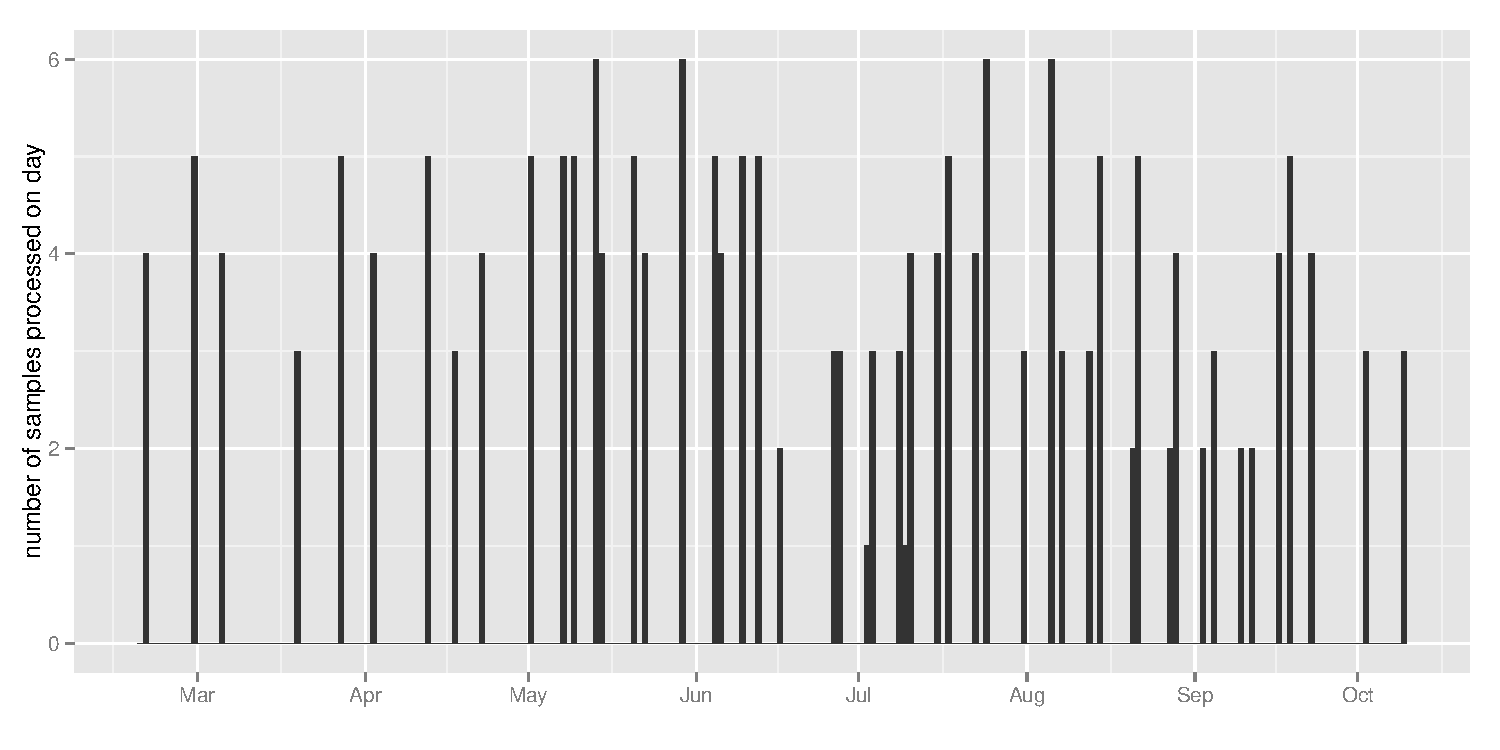
\includegraphics[scale=.5] {flowdatasets/figures/il2ra-samples-time.pdf}
\mycaption{figure:IL2RA-sample-time} 
{Number of samples analysed per day.}
{
A total of 195 (180 + 15 repeats) samples were analysed over seven months (from March to October).
During that period, samples were analysed on $51$ days,
with between one and six samples analysed each day.
}
\end{figure}


The cell phenotypes studied by \citet{Dendrou:2009dv}, were obtained using manual gating with the FlowJo software\footnote{\url{www.flowjo.com}}.
Manual gating follows the current state of knowledge of immune cell lineages (\Cref{figure:manual-gating-strategy}).
Lymphocytes are distinguishable from more granular and larger cell types based on forward and side scatter.
The lymphocytes include, B cells and T cells, and the latter population includes cells expressing \protein{CD8} or \protein{CD4}.
Within the lymphocytes, the subset expressing \protein{CD4} are defined as T lymphocytes.
The \protein{CD4}\positive T lymphocyte subset can be further divided into regulatory and non-regulatory cells (\Cref{figure:manual-gating-strategy}c).
Regulatory cells represent a low-frequency subset which has the highest CD25 expression compared to other cells at rest, and which
expresses no or only a very low level of \protein{CD127}.  
%higher in \protein{CD25} and lower in \protein{CD127}.
Regulatory T cells can be defined more precisely by the intracellular \protein{FOXP3} transcription factor, which is constitutively expressed
only in regulatory T cells.
Non-regulatory T cells represent a larger proportion of T lymphocytes.
They express more \protein{CD127} and less \protein{CD25} than regulatory T cells.
Non-regulatory T cells can be further divided into naive and memory subsets (\Cref{figure:manual-gating-strategy}d).  
Upon antigen presentation, naive cells are activated and differentiate into effector cells, some of which further differentiate into memory cells
while the remainder die.
%Thus cells are in a transitional state between naive and memory.  
As part of the transition process from naive to memory, the cell surface protein \protein{CD45RA} is lost so that consequently naive cells have higher \protein{CD45RA} expression than memory cells.
A further difference between these subsets is that memory cells tend to have a higher CD25 expression than naive cells.
%A further secondary distinguishable property is that memory cells tend to be higher in \protein{CD25} expression than naive cells.
Since \protein{CD25} expression on the naive cells is low, with only a subset of the cells expressing substantial levels of the molecule,
\citet{Dendrou:2009dv} define a threshold above which naive cells are deemed positive for CD25.
Their threshold is defined in terms of an isotype control, a sample not stained for \protein{CD25}, to measure the background.


The threshold for positivity was defined using an isotype control sample which was stained not with anti-CD25 antibody but with an antibody
with no defined target which was conjugated to the same fluorochrome, APC (\Cref{table:IL2RA-panel}), thereby enabling the background level of any unspecific
staining to be observed.

The variation observed through time complicates the task of gating, which may already be influenced by the fact that gating is subjective as it relies,
to an extent, on the opinion of the gater.  The time-dependent variation is, for example, observeable from the MFI of the memory population and this can
be corrected using beads.  But the reliance on manual gating is more difficult to deal with and it has been questioned how good isotype controls are.
The use of beads might help overcome the abolute need for isotypes, especially when dealing with cells with a low Fc receptor expression where
unspecific antibody binding is less of an issue.
However, even the bead populations themselves require gating, and so in the first section of the chapter...

the variables contributing to phenotypic variation are genotype, age and sex (examples), but alos experimental temporal variation as well
as that introduced by gating, whic are then focusing on more...


%adjusted depending on the MFI of the blank beads population on that day.
%\protein{CD25} is known to be upregulated under inflammatory conditions

I think that in this paragraph you perhaps need to describe what the problem is or convey why there is a need for automated gating ie: the variation observed through time complicates the task of gating, which may already be influenced by the fact that gating is subjective as it relies - to an extent - on the opinion of the gater.
This time-dependent variation is, for example, observable from the MFI of the mem pop and this can corrected using the beads.
But the reliance on manual gating is more difficult to deal with and it has been questioned how good isotype controls are.
The use of the beads might help overcome the absolute need for isotypes, especially when dealing with cells with a low Fc receptor expression where unspecific antibody binding is less of an issue.
However, even the beads populations themselves require gating, and so in the first section of the chapter you show how…etc etc


Since samples were collected and analysed over a period of seven months, 
instrument variation is detectable in the CD25 mean fluorescence intensity (MFI) of the memory cell population (\Cref{figure:memory-CD25MFI-time-effect}).
This time effect was first discussed in \citet{Dendrou:2009bl}.
To correct for this, beads were run daily in order to define a transform from MFI to molecules of equivalent fluorescence (MEF) which should be more stable over time.
The bead data consist of six populations of increasing fluorescence intensity, which are manually gated by \citet{Dendrou:2009dv}.
These gated bead populations can also be used to define a threshold above which cells are considered positive for \protein{CD25}.

In the first section of this chapter, I will show how to gate the bead data automatically.
Next I will move on to the harder task of the automatic gating of some of the cell phenotypes studied by \citet{Dendrou:2009dv}.
% Calli's results
% cell phenotypes
Two of these cell phenotypes, percent of \protein{CD25}\positive naive cells and CD25 MFI of memory cells, were found to be associated with SNPs near the \gene{IL2RA}.

It might worth incorporating these points into a broader discussion regarding variables in the paragraph above - you could explain that the variables contributing to phenotypic variation of the data set are genotype, age and sex - stating the examples you mention - and also experimental/temporal variation as well as that introduced by gating - which are then focusing on more...

Percent of \protein{CD25}\positive naive cells and percent of memory cells, were found to be associated with age and marginally associated with sex.
The repeatability was also tested thanks to the 15 recalled individuals.
Repeatability is important because better repeatability improves the power to detect an effect.
These repeatability and association results, as reported by \citet{Dendrou:2009dv}, are summarised in \Cref{table:calli-results}.  
In this chapter I will assess, whether I can replicate or improve on these results, with special attention given to repeatability,
by replacing the last two univariate manual gating steps (\Cref{figure:manual-gating-strategy}d)
with a computational method:
%Manual gating follows a step-by-step hierarchical process.
%Ideally the entire manual gating process should be replaced by an automatic algorithm.
%But in order to facilitate initial comparison with manual gating, in this chapter,
%I will only automate the two last univariate gating steps (\Cref{figure:manual-gating-strategy}d):
\begin{itemise}
\item Univariate gating on \protein{CD25} to threshold naive cells into positive and negative subsets, in order to obtain the percentage of CD25\positive naive cells.
\item Univariate gating on \protein{CD45RA} to threshold non-regulatory T cells into naive and memory cells, in order to obtain the percentage of memory cells and
the CD25 MFI of memory cells.
\end{itemise}


\begin{figure}[h]
\centering
\includegraphics[scale=.5] {IL2RA/figures/ManualGating/manual-gating.pdf}
\mycaption{figure:manual-gating-strategy} 
{Manual gating of IL2RA dataset.}
{
Manual gating strategy to extract memory T cells and CD25\positive naive T cells (green boxes).
Note that the CD45RA gates exclude cells which are considered to be neither memory nor naive.
Our automated gating replaces the final stage of the manual gating on CD25 and CD45RA.
}
\end{figure} 


\begin{figure}[h]
\centering
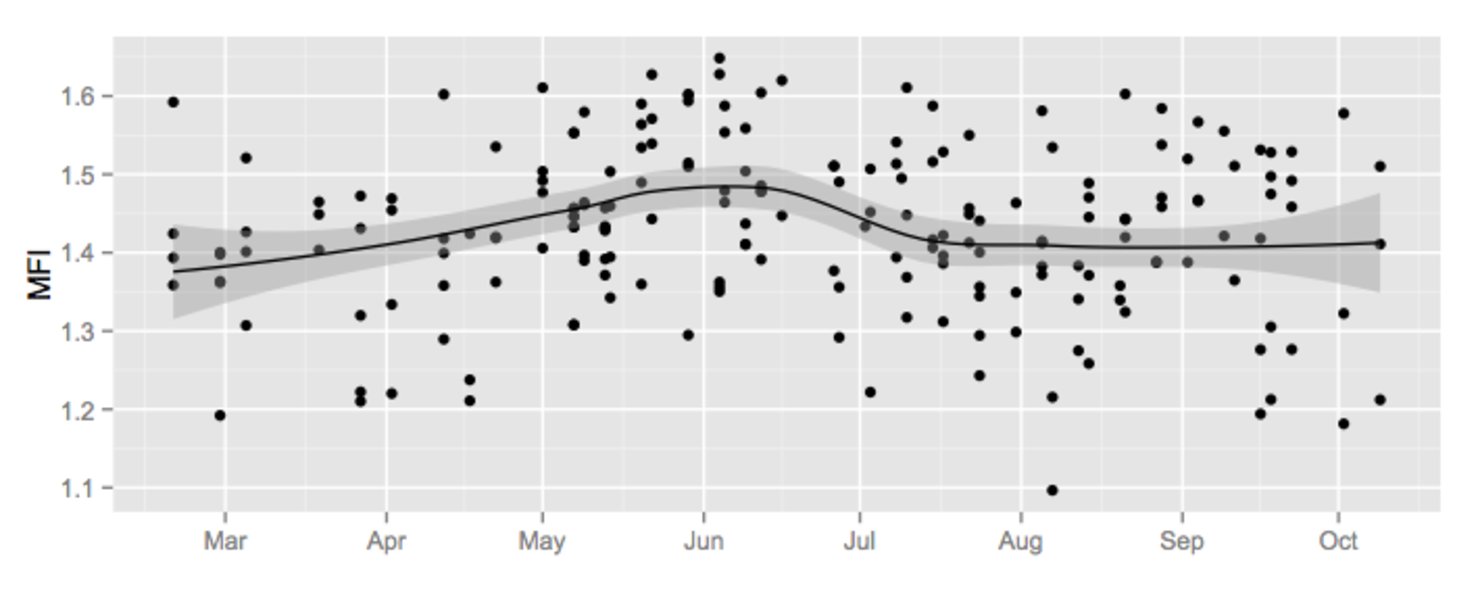
\includegraphics[scale=0.6]{IL2RA/figures/CD25-mfi-time-effect.pdf}
\mycaption{figure:memory-CD25MFI-time-effect}
{Effect of time on CD25 MFI in memory cells.}
{
\protein{CD25} MFI of memory cell population (manually gated) over time of experiment.
The black line represents the loess regression line.
Samples analysed after July tend to have a lower CD25 MFI than those analysed before.
}
\end{figure} 




%CD101,CD127,CD25_MA251+2A3,CD4,CD45RA,HLADR
%CD127,CD25_MA251+2A3,CD4,CD45RA,ISO 



%%% BEADS
\section{Univariate clustering of bead data}

In flow cytometry, a method of normalising fluorescence intensity to account for instrument variation, is to convert the \gls{MFI}
measured on a population to \gls{MEF} \citep{Schwartz:1996jj,Dendrou:2009bl}.
In order to apply this conversion, specially designed beads of known and (assumed) constant fluorescence defined in terms of \gls{MEF}, are used as a reference.
The MEF property of these beads is deemed stable whereas the MFI of the bead population is dependent on the instrument and varies over time.

The beads used here are specially manufactured so that they belong to six distinct populations of increasing MEF as shown in \Cref{table:fluorospheres}.
Following the bead manufacturer's guidelines, plotting the $\log_{10}(MEF)$ of these six bead populations against
the corresponding calculated $\log_{10}(MFI)$ from the gated bead populations, we fit the linear regression:

\begin{equation}
    \log_{10}(\text{MEF})=\beta \times \log_{10}(\text{MFI}) + \alpha
\label{equ:MEF}
\end{equation}

The MEF is in fact a power transform of the MFI (only defined for strictly positive MFI values):

\[
    \text{MEF}= 10^\alpha \times \text{MFI}^\beta
\]

The original MEF transform used by \citet{Dendrou:2009bl} assumes that $\beta=1$,
although I relax that assumption.
%which gives similar results given that I found that the $\beta$ term in \Cref{equ:MEF} turns out to be on average $0.96$.

In calculating the slope $\beta$ and the intercept $\alpha$ parameters of the linear model,
only the five brighest bead populations are used because the MEF of the blank beads is not specified by the manufacturer.
%In fact extrapolating the MEF of the blank beads yields the detection threshold (\Cref{figure:mef}) which we will see in the next section,
However, as we will see in the next section, the blank beads can be used to define a threshold for positivity.
%The MEF of the blank beads is always greater than the intercept $\alpha$  which represents the log offset (the zero channel value).
%Below this threshold the intensity is meaningless as the blank beads contain by design no fluorochrome.

Typically bead data are gated manually.
Here, in order to obtain the parameters of the MEF transform, I will use an automatic process to gate the beads.

Since all beads are manufactured to be of identical dimensions, we expect a single cluster in the scatter channels: the singlet bead population.
Events which lie away from the singlet population are deemed to be beads clumped together or debris and so are discarded.
Filtering of singlets can be achieved by fitting a bivariate normal distribution on forward and side scatter and only keeping
points within the 95th percentile.
Having gated the singlets, I subset the data and proceed to gate on the fluorescence channels to identify the six bead populations.
Given that the number of bead populations is known, that the bead signal is sufficiently clear and that the number of events is small (in the order to 10,000),
I use the K-medoids algorithm (\Cref{appendix:clustering}).
The solution has been implemented in the \Rpackage{flowBeads}, available on BioConductor.
Automatic gating shows near perfect agreement with manual gating (\Cref{figure:bead-agreement}) and so is now the established method of analysing
bead data in our lab.
Applying the bead normalisation to the memory CD25 MFI from \Cref{figure:memory-CD25MFI-time-effect}, we improve on the repeatability of that 
cell phenotype from $r^2=0.959$ to $r^2=0.994$, where $r^2$ is the Pearson correlation squared (\Cref{figure:CD25-MFI-beads-normalised}).

\begin{table} [hb]
\begin{center}
\begin{tabular} {|c c c c c c|}
\cline{1-6}
Population  & FITC    & RPE     & REP-Cy5 & \textbf{APC}     & PE-Texas Red\\
\cline{1-6}
1           & B       & B       & B       & \textbf{B}       & B \\
2           & 2,500   & 1,500   & 750     & \textbf{4,100}   & 552\\
3           & 6,500   & 4,400   & 2,100   & \textbf{10,300}  & 2,014\\
4           & 19,000  & 14,500  & 6900    & \textbf{25,500}  & 6,975\\
5           & 55,000  & 43,800  & 22,100  & \textbf{67,300}  & 20,685\\
6           & 150,000 & 131,200 & 77,100  & \textbf{139,100} & 71,888\\
\cline{1-6}
\end{tabular}
\end{center}
\caption{
\label{table:fluorospheres}
\textbf{FluoroSpheres from DakoCytomation.}
The Molecules of Equivalent Fluorochromes (MEF) values for the six bead populations as provided by the manufacturer.
B denote the blank beads which by design contain no fluorochrome.
Of the six fluorochromes contained by each bead only APC is used in the experiment.
}
\end{table}

\begin{figure}[hb]
\centering
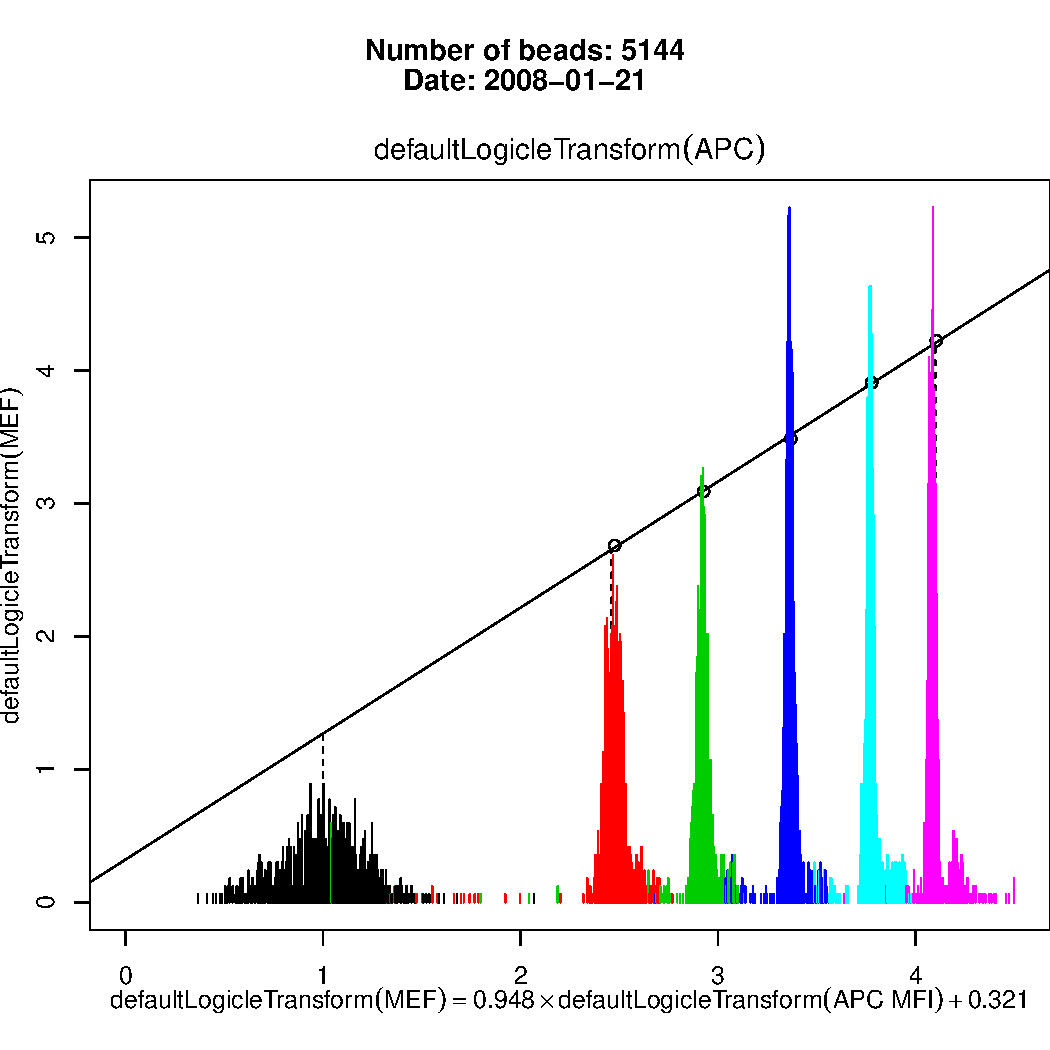
\includegraphics[scale=.5]{IL2RA/figures/Beads/flowBeads.pdf}
\mycaption{figure:mef}
{ Linear regression of bead APC MEF against the APC MFI as defined in \Cref{table:fluorospheres}.}
{
The six peaks represent the six bead populations.
%The horizontal dash lines represent the MEF of the six bead populations.
%The red and green vertical lines define the range of memory CD25 MFI across all samples in \citet{Dendrou:2009dv}.
These types of plots are generated automatically by the \Rpackage{flowBeads}.
}
\end{figure}


\begin{figure}[hb]
\centering
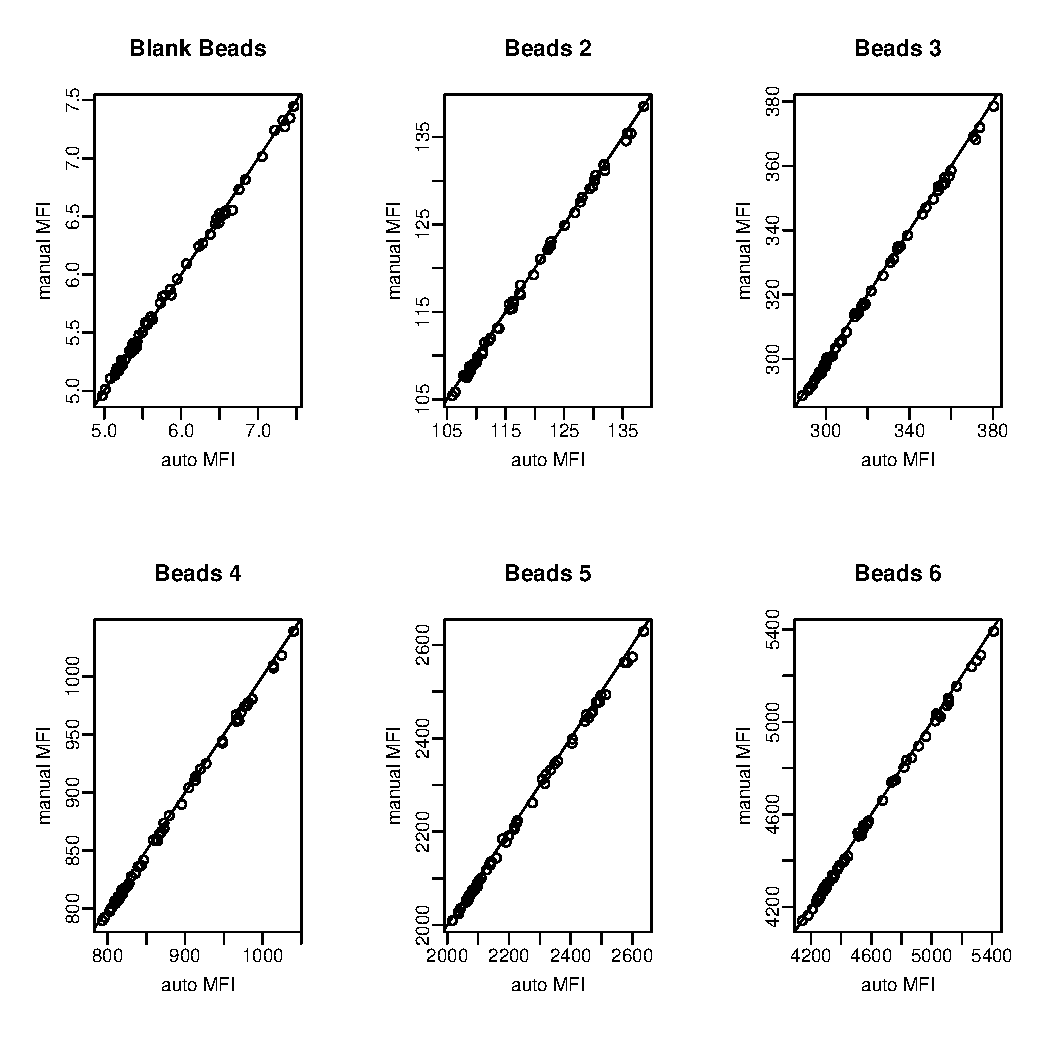
\includegraphics[scale=0.6]{IL2RA/figures/Beads/manual-auto-mfi.pdf}
\mycaption{figure:bead-agreement}
{ Comparison of bead population MFI using manual and \texttt{flowBeads} gating.  }
{ There is good agreement of the APC MFIs of the six bead populations identified with manual and using the automatic approach. }
\end{figure}



\begin{figure}[ht]
\centering
\begin{subfigure}[b]{.4\textwidth}
    \centering
    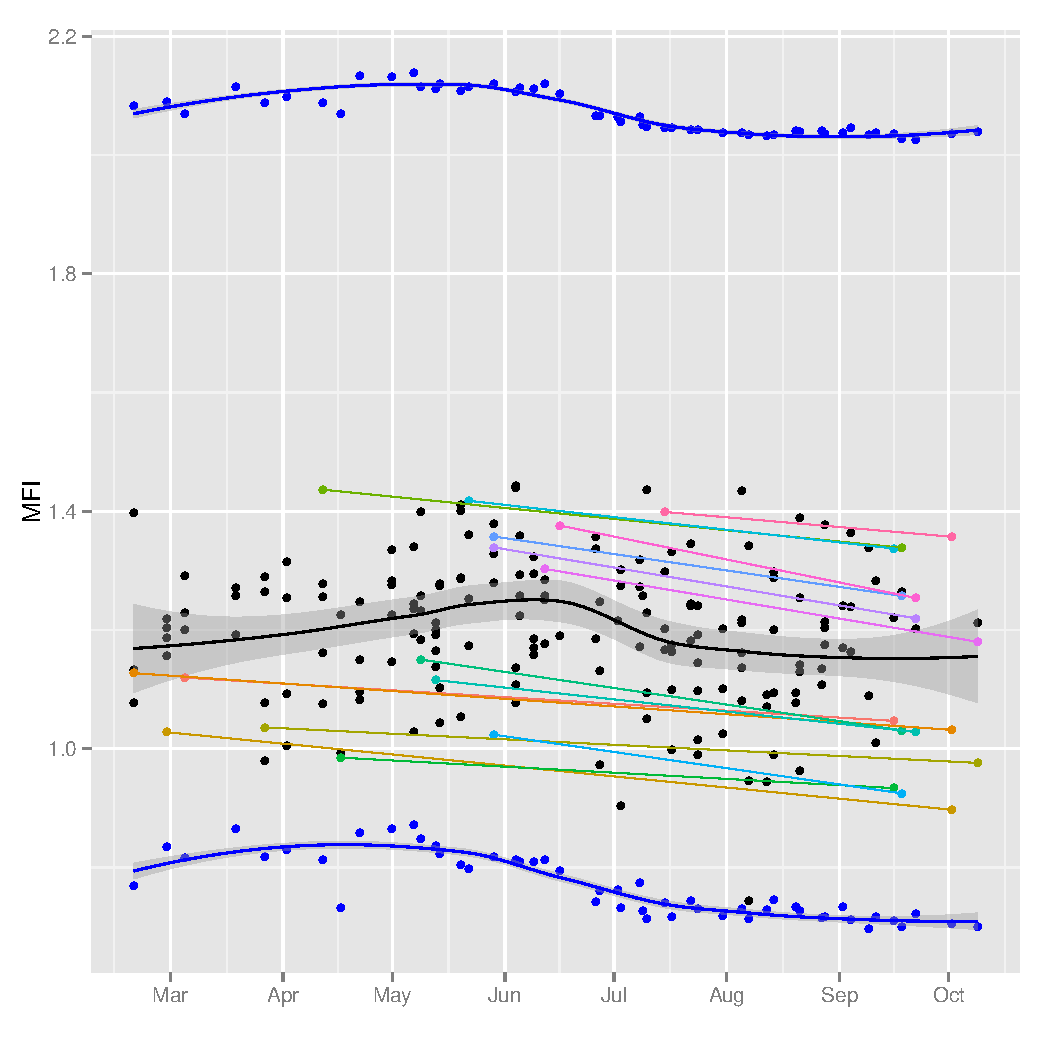
\includegraphics[scale=.3]{IL2RA/figures/CD25-MFI-time-effect-repeatability.pdf}
    \caption{Unormalised}
\end{subfigure}
~
\begin{subfigure}[b]{.4\textwidth}
    \centering
    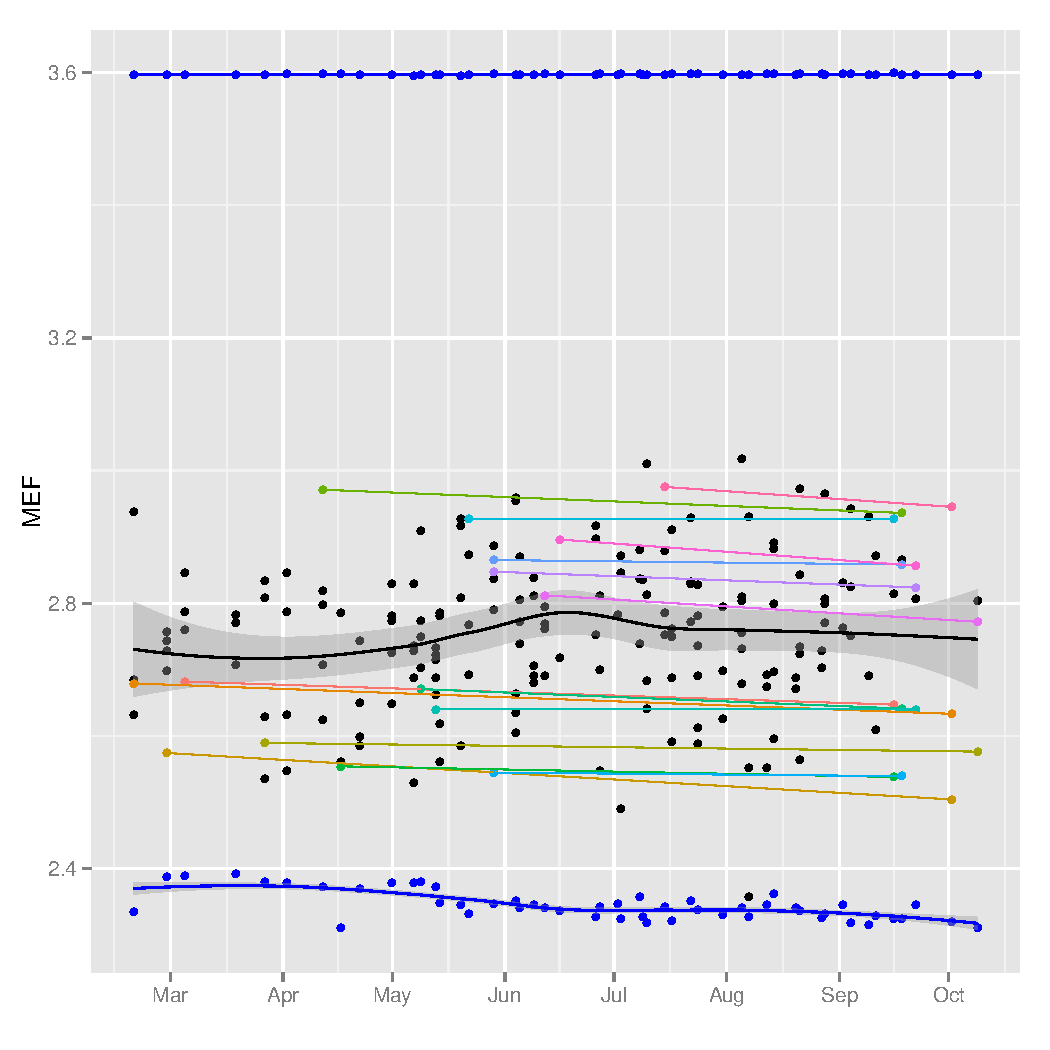
\includegraphics[scale=.3]{IL2RA/figures/CD25-MFI-time-effect-beads-normalised.pdf}
    \caption{Normalised}
\end{subfigure}
~
\begin{subfigure}[b]{.4\textwidth}
    \centering
    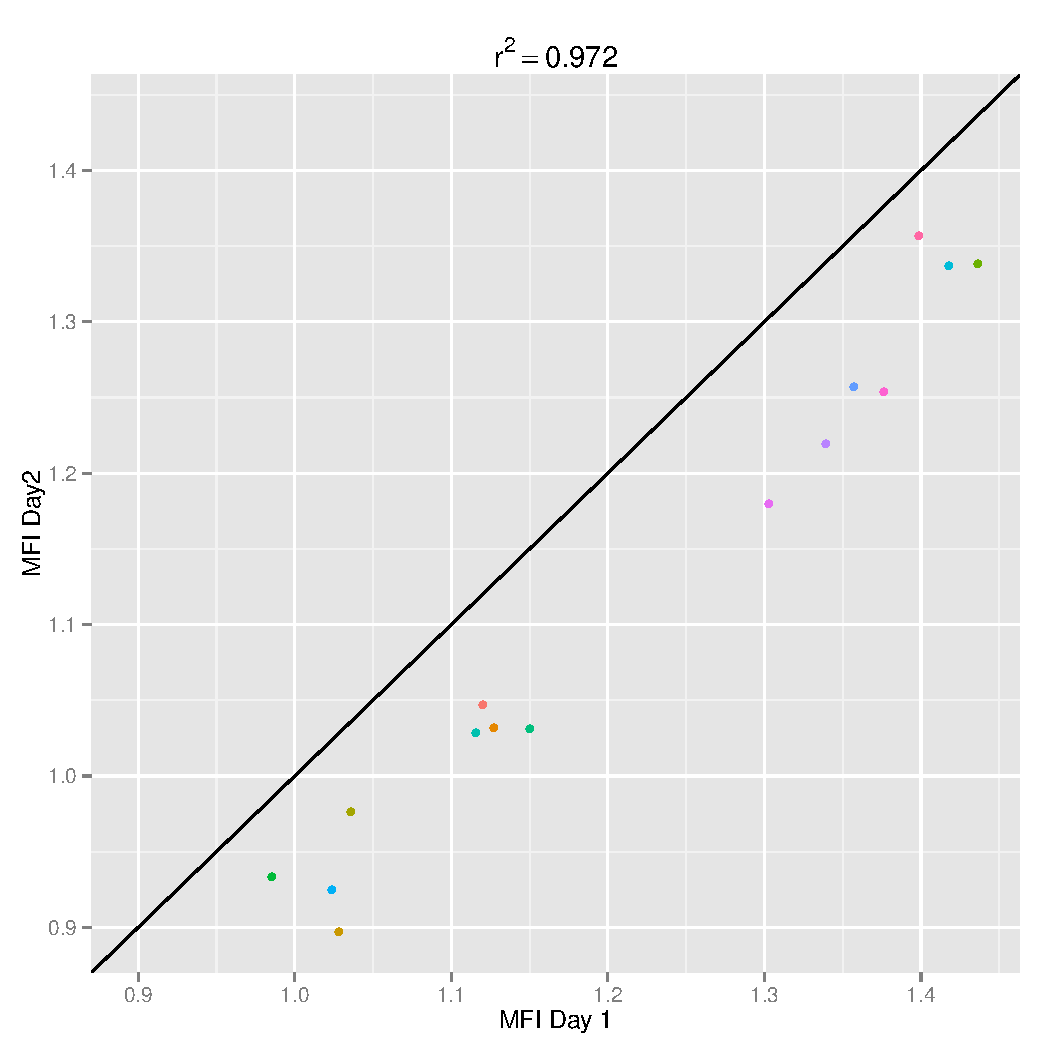
\includegraphics[scale=.3]{IL2RA/figures/CD25-MFI-repeatability.pdf}
    \caption{Unormalised: $r^2=0.959$}
\end{subfigure}
~
\begin{subfigure}[b]{.4\textwidth}
    \centering
    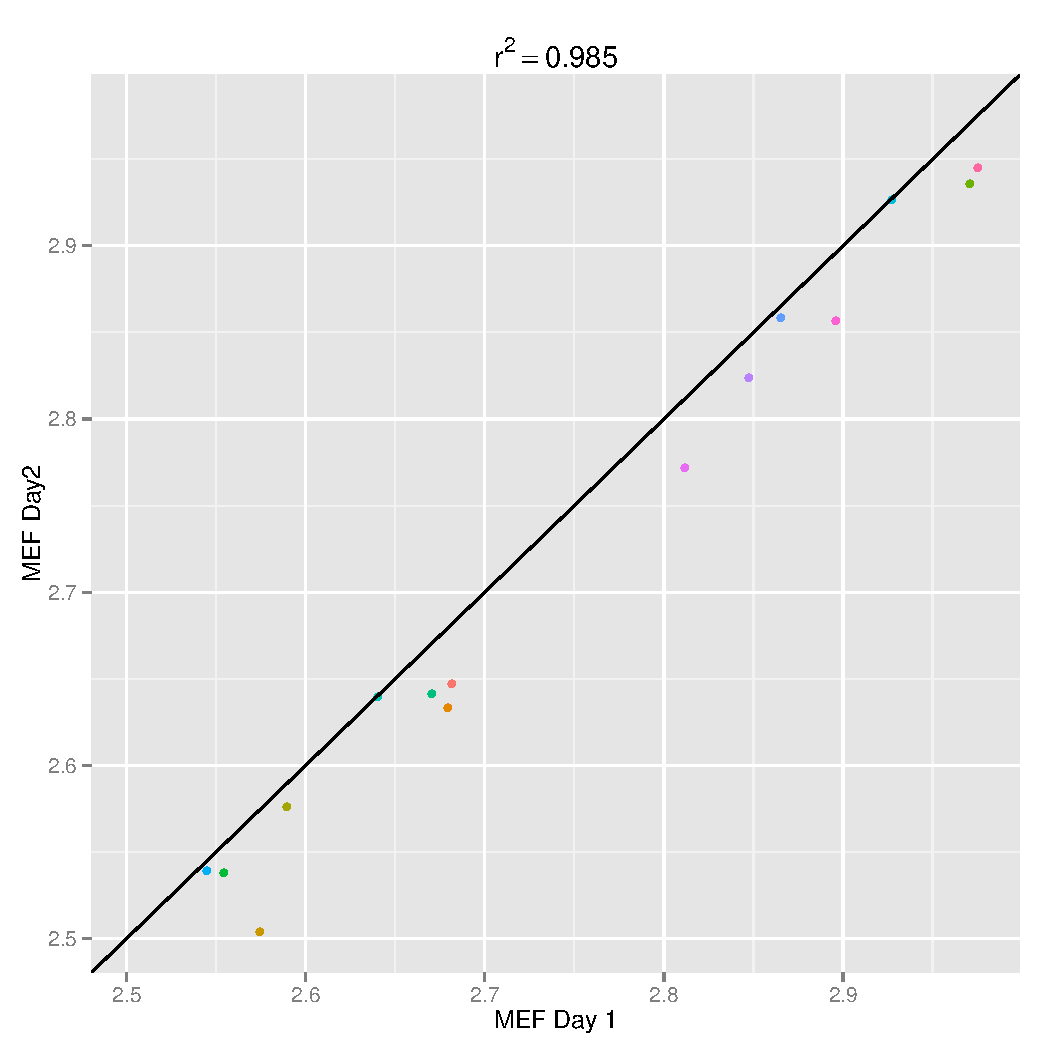
\includegraphics[scale=.3]{IL2RA/figures/CD25-MFI-beads-normalised.pdf}
    \caption{Normalised: $r^2=0.994$}
\end{subfigure}
\mycaption{figure:CD25-MFI-beads-normalised}
{Bead normalisation partially corrects for long term time effect in CD25 MFI of the memory cell population.}
{
  In \textbf{(a)} and \textbf{(b)}, the blue points represent the \protein{CD25} MFIs of the two lowest bead populations,
  in black the \protein{CD25} MFIs of the memory cell populations.
  The dashed blue lines represent the overall mean of each the two bead populations.
  A loess regression is fitted to the MFIs of the beads and memory cells to illustrate the MFI variation over days.
  The points joined by lines are memory cell \protein{CD25} MFIs from the $15$ recalled individuals (\Cref{table:IL2RA-recalled-individuals}).
%The normalisation step involves aligning the peaks of the two bead populations across days to the overall mean of each of the populations (the dashed blue).
  The bead normalisation transform \Cref{equ:MEF} improves the repeatability of the MFI in recalled individuals from $r^2=0.959$ \textbf{(c)} to $r^2=0.994$ \textbf{(d)}.
}
\end{figure}




%%% CD25POS
\section{Univariate gating on CD25: defining a \protein{CD25}\positive threshold on naive cells}

%The population of non regulatory CD4\positive T cells is not clearly bimodal on CD25 like CD45RA.
The approach adopted by the manual method is to define a threshold above which cells are considered positive for CD25.
According to \citet{Dendrou:2009dv} (and \contributor{Calliope Dendrou} personal communication),
the CD25\positive threshold is set manually using an ad-hoc process based on an isotype control, bead data and ultimately a judgement call
by the manual gater.
An isotype control is a sample stained with the same fluorochrome (APC) but conjugated to a
non-specific antibody not designed to target the marker we are interested in quantifying.
It is used as a technique for assessing background APC fluorescence not resulting from CD25 binding.

%adjusted using the daily bead data.
This manual approach to setting the threshold, leads to a different gate position per sample per day (\Cref{figure:cd25pos-gates}).
We notice that on some days there is greater variability in the positions of the gates.
Also, there is the same downwards time-trend in the position of the gates observed in (\Cref{figure:memory-CD25MFI-time-effect}).
%which can be explained by position of the gates needing to be shifted down to account for this (\Cref{figure:memory-CD25MFI-time-effect}).

\begin{figure} [h]
\centering
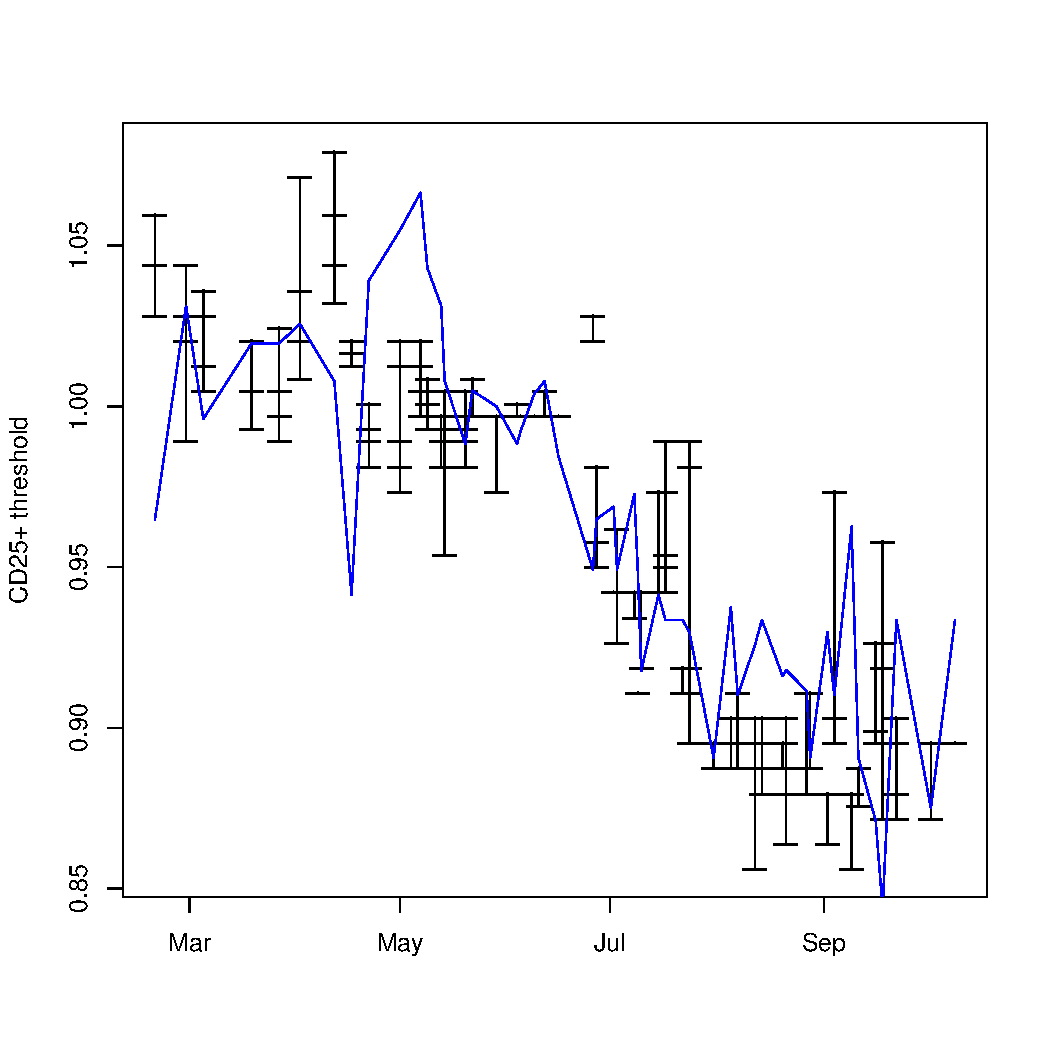
\includegraphics[width=.5\textwidth] {IL2RA/figures/cd25pos-gates.pdf}
\mycaption{figure:cd25pos-gates}
{Position of the \protein{CD25}\positive gate over duration of experiment.}
{
The black horizontal dashes are the positions of the manual CD25\positive gates for all 196 samples over the time course of the experiment (51 days).
The vertical black lines represent the days and so define the range of the manual gate positions on a given day.
The blue line represents our automatic CD25\positive gate which corresponds to the $86^{th}$ percentile of the blank bead population.
}
\end{figure}


%As we can see from \Cref{figure:mef}, the Memory T Cell MFI range is in between the MFI of the blank beads and dimmest bead population.
%Our automatic approach relies 
%Thus we define a threshold to distinguish CD25\positive from CD25 negative cells using the automatically gated bead data on the day which the sample was ran.
Drawbacks of the manual approach are its lack of consistency and its reliance on isotype controls.
The gating criterion is subject to human judgement and so may not be consistent across samples.
Isotype controls are costly since part of the sample and fluorochromes is consumed for control purposes, consequently they are not always used.
Also they are not necessarily an accurate measure of background fluorescence since
they are also a source of noise linked to differences in the constitution of the control sample,
the behaviour of the staining and other sources of technical variation \citep{Maecker:2006ft}.

I wished to improve on this process by using a more consistent and economical approach, using only beads, which I called \texttt{beads.thresh}.
Instead of using isotype data, my working hypothesis,
was that blank beads would constitute a more stable reference, which can be used to define an APC-CD25 threshold.
To find a suitable bead-derived threshold, I first gated the blank beads using my \Rpackage{flowBeads}, then I searched for the APC percentile of the
blank bead population which best agreed with the manual gate (\Cref{figure:cd25pos-gate-agreement}).
I found that in this dataset, the $86^{th}$ percentile of the blank bead population, best matched the manual gate position.

\begin{figure}[h]
\centering
  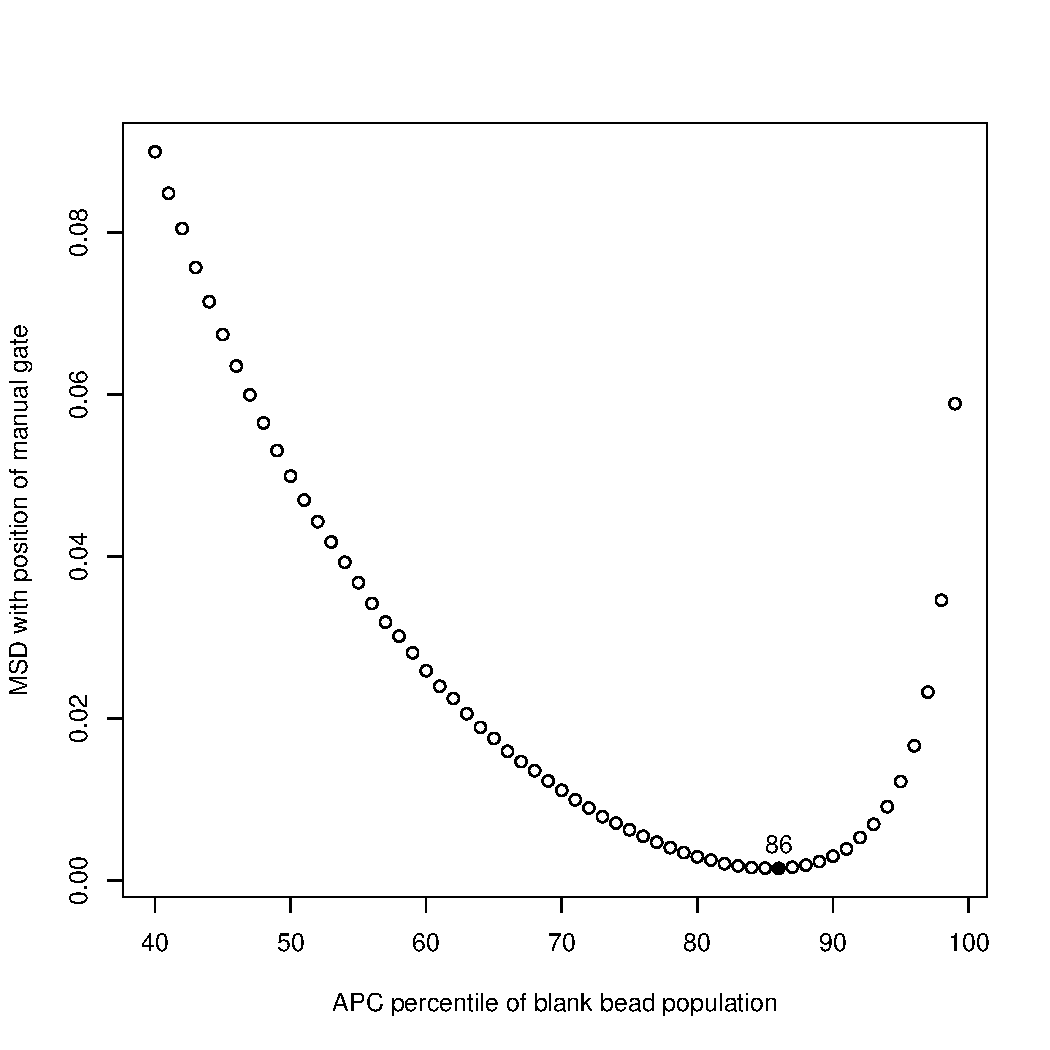
\includegraphics[width=.5\textwidth]{IL2RA/figures/cd25pos-gate-agreement.pdf}
\mycaption{figure:cd25pos-gate-agreement}
%{ Agreement of blank bead derived gate position with manual. }
{ Comparison of the blank bead derived gate position with the manual equivalent. }
{
On the x axis, the APC-CD25 percentiles of the blank bead population from 40 to 99.
On the y axis, the mean squared difference between the position of the manual gate and that of the bead-derived gate for that percentile threshold.
The $86^{th}$ percentile yields the lowest mean squared difference hence the best agreement with the manual gating.
The automatic threshold selection method (\texttt{beads.thresh}) is therefore defined as the APC $86^{th}$ percentile of the blank beads population.
}
\end{figure}

\begin{figure}[h]
\centering
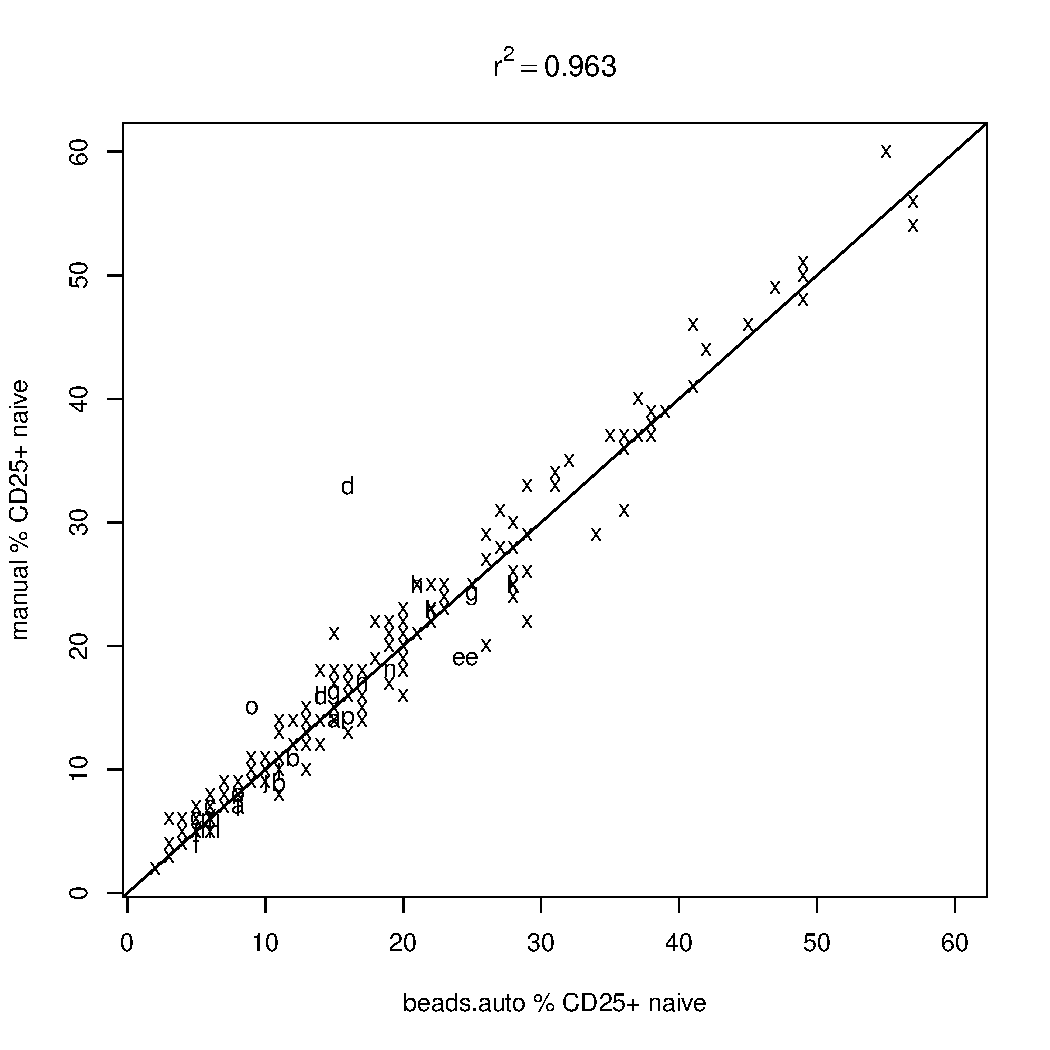
\includegraphics[width=.5\textwidth]{IL2RA/figures/naive-cd25pos-beads-manual-agreement.pdf}
\mycaption{figure:threshold-manual-agreement}
{ Agreement with manual of percentage of \protein{CD25}\positive naive cell phenotype. }
{
  Except for individual d, the agreement of \texttt{beads.thresh} with manual for percentage of CD25\positive naive cells
  is very good.  $r^2$ is the Pearson correlation squared.
}
\end{figure}

Hence the CD25\positive threshold defined by my approach, \texttt{beads.thresh}, is set as the $86^{th}$ percentile of the automatically gated blank bead population on that day.
As we only have one bead set per day, we have a single fixed CD25 gate for all samples on that day (\Cref{figure:memory-CD25MFI-time-effect}).

%In order to assess the dependency of the repeatability on the gates we chose the percentage phenotypes rather than the MEF.
%The concept of repeatability is explained in Appendix~\Cref{repeatability}.
The \texttt{beads.thresh} method for setting \protein{CD25} thresholds  shows improved repeatability of the percentage of \protein{CD25}\positive naive T cell phenotype
than manual (\Cref{figure:repeatability-cd25pos-naive}).  

%One question that might be expected is what would happen if you used automated gating on the isotype and then effectively applied that to the CD25-stained samples?
%A skeptic could argue that  isotype controls might look a bit more variable but that is because they are capturing sample-specific difference, which the beads of course cannot do.
%I'm not saying that I necessarily buy that argument are that you would need to do any further analysis, but I guess it is still a valid question to be aware of.


\begin{figure}[h]
\centering
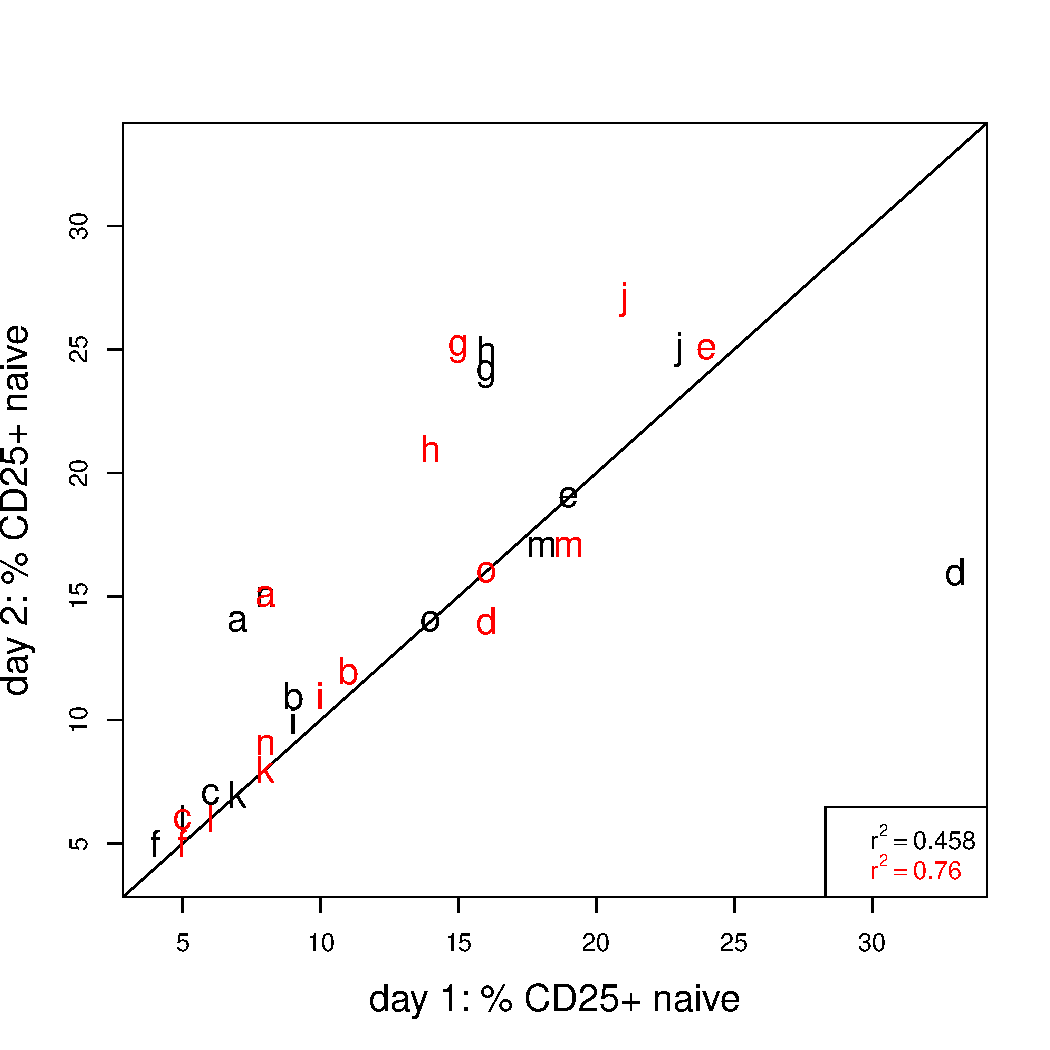
\includegraphics[width=.5\textwidth]{IL2RA/figures/repeatability-cd25pos-naive.pdf}
\mycaption{figure:repeatability-cd25pos-naive}
{ Repeatability of percentage of naive \protein{CD25}\positive. }
{
Repeatability of the percentage of naive cells which are CD25\positive from day one to day two.
The overall repeatability of this cell phenotype was better with \texttt{beads.thresh} (red)
than the manual (black).
Letters are used to identify indidividuals, see \Cref{table:IL2RA-recalled-individuals}.
The Pearson correlation squared is $r^2=0.458$ for manual and $r^2=0.769$ for \texttt{beads.thresh}.
}
\end{figure}

\clearpage

%%% CD45RA
\section{Univariate gating on CD45RA: fitting two-component mixtures on non-regulatory T cells}

Non-regulatory CD4\positive T cells appear bimodal with respect to CD45RA expression,
because this marker is lost upon activation of naive cells (CD45RA\positive) to memory cells (CD45RA\negative).
In this section, we will model the CD45RA distribution by fitting a two component mixture model.
Although we model both populations, we will only gate the memory (CD45RA\negative) cell population, which corresponds to the first component,
since the naive (CD45RA\positive cell population, the second component, is not a terminal gate as
it is further divided into CD25 negative and positive subsets (see previous section).


%First, I will try a two univariate Gaussian distributions, then I will try a more flexible mixture of two symmetric distributions.
%To this purpose, I used the \Rpackage{mixtools}  which provides an implementation of the \Gls{EM} algorithm \citep{Dempster:1977ul}
%to fit Gaussian (\Rfunction{normalmixEM}).
In order to model the bimodal CD45RA distribution, I use the \Rfunction{normalmixEM} function in the \Rpackage{mixtools},
which provides an implementation of the \Gls{EM} algorithm \citep{Dempster:1977ul}.
The parameters, mean, variance and component weight, of the two-component Gaussian mixture model,
are first initialised by the K-medoids algorithm (\Cref{appendix:clustering}).
The parameter estimates are then obtained  by running the EM algorithm until convergence.
I call this method \texttt{mm}.
%Because we are only dealing with a mixture of two distributions only one mixing parameter needs to be estimated since the other is simply its complement.
%The other parameters to be estimated are the parameters of the distribution such as the mean and the variance when fitting a mixture of Gaussians or simply the location parameter
%for the semi-parametric distributions..
%More general distributions which are also symmetric
%Semiparametric symmetric distributions are kernel density estimates centered around a location parameter.
%The bandwidth parameter of the kernel density estimate is fixed to $0.1$ but could also have been estimated heuristically from the data.

\subsection{Using the mixing proportions of the mixture model}

Instead of emulating manual gating with thresholding, I will now try a different approach, using the mixing proportions obtained from \texttt{mm}.
I will also apply a more flexible mixture model, a semi-parametric symmetric distributions (\Rfunction{spEMsymloc}) again from the \Rpackage{mixtools}.
I will call this method \texttt{spmm}.
%Returns semiparametric EM algorithm output (Bordes et al, 2007, and Benaglia et al, 2009) for location mixtures of univariate data and symmetric component density.
%The other parameters to be estimated are the parameters of the distribution such as the mean and the variance when fitting a mixture of Gaussians or simply the location parameter
%for the semi-parametric distributions..
%More general distributions which are also symmetric
Semiparametric symmetric distributions are kernel density estimates centered around a location parameter.
The bandwidth parameter of the kernel density estimate is fixed to $0.1$ but could also have been estimated heuristically from the data.

We can see that both automatic mixture model approaches, \texttt{mm} and \texttt{spmm}, yield worse repeatability than manual (\Cref{figure:repeatability-memory-weights}).
As is the case for the sample from individual d on day one (\Cref{figure:cd45ra-threshold-example}),
the repeatability is compromised when the mixture of distributions approach fails to find a suitable gate because of poor model fit.
%As the same individual shows a very different profile on day two, I believe that, in this case, the noise is due to technical variation on that day rather
%than true biological variation.
%\subsection{Improved Repeatability when Averaging Gate Positions}

\begin{figure}[h]
\centering
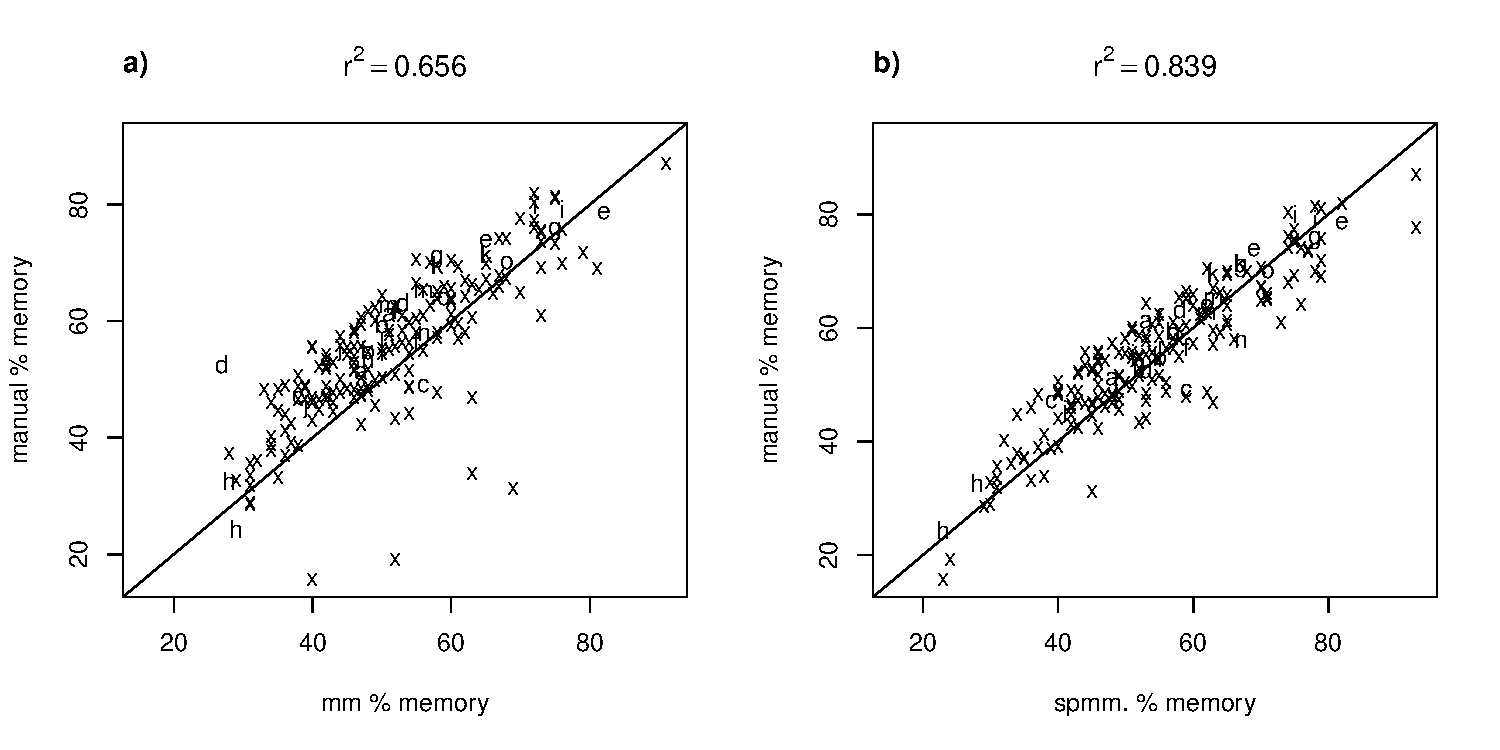
\includegraphics[scale=.5]{IL2RA/figures/memory-auto-manual-agreement-weights.pdf}
\mycaption{figure:repeatability-memory-weights}
{Agreement with manual of the percent memory cell phenotype obtained with \texttt{mm} (a) and \texttt{spmmm} (b).}
{
  The more flexible model, \texttt{spmm}, tends to agree better with percent memory cell phenotype returned by manual, than \texttt{mm}.
  %\texttt{mm} tends to report a higher percentage of memory cells than reported by manual.
  Again we can see in (a), that \texttt{mm} underestimates the percentage of memory cells in individual d compared to
  manual.

}
\end{figure}



\begin{figure}[h]
\centering
  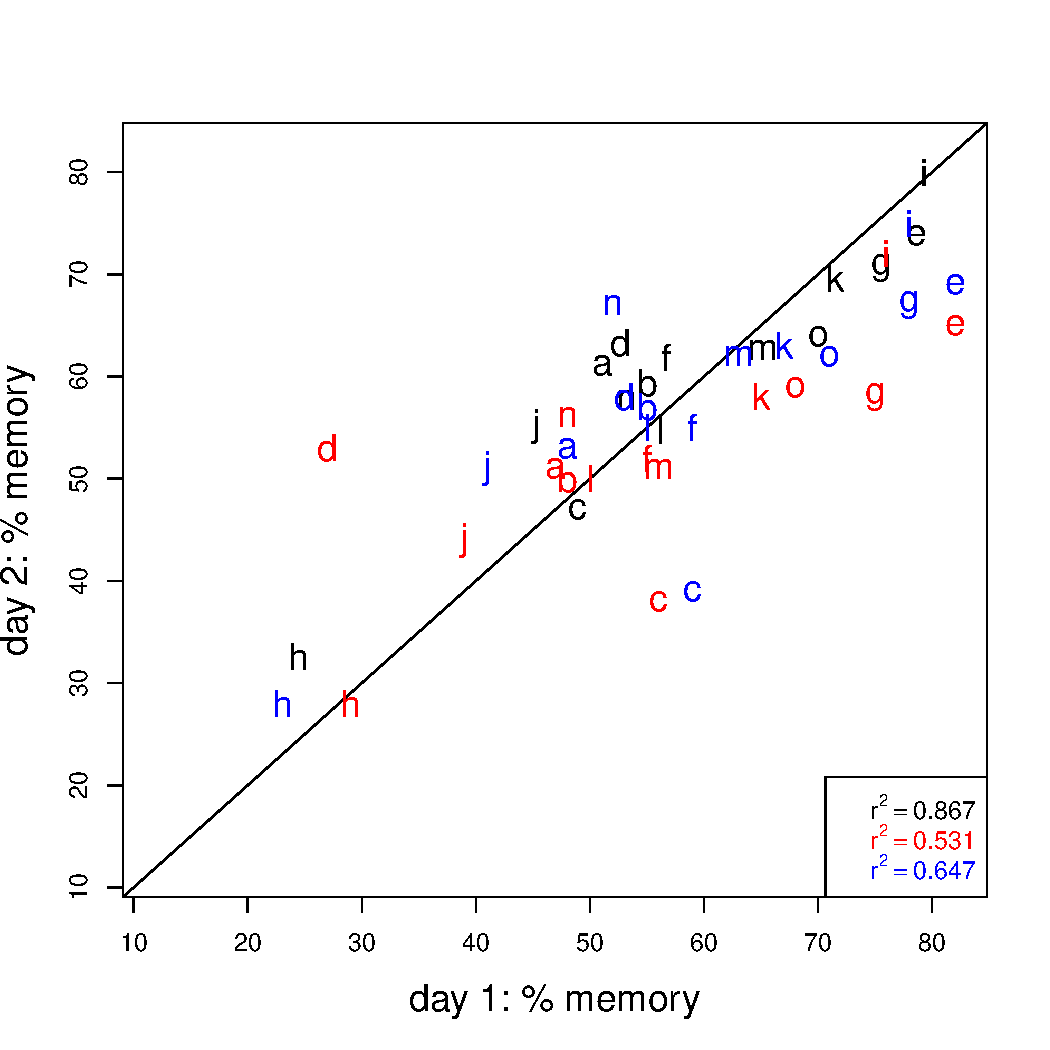
\includegraphics[width=\textwidth]{IL2RA/figures/repeatability-memory-weights.pdf}
\mycaption{figure:repeatability-memory-weights}
{Repeatability of the percent memory cell phenotype with manual (black), \texttt{mm} (red) and \texttt{spmm}.}
{
  While manual still shows the best repeatability, the repeatability of the automatic methods is quite encouraging, given
  these have no knowledge of the manual gates and are based purely data driven.
  Also as seen using the thresholding methods, individual d is a clear outlier when gated with the \texttt{mm} method.
}
\end{figure}




\subsection{Emulating manual gating by picking a threshold}

The manual gating of memory cells, defines a threshold on the bimodal CD45RA distribution below which cells are regarded as CD45RA-.
Here, I attempt to emulate manual gating by defining a threshold on the fitted two-component mixture model.
%later, I will consider using the mixture weights.  
I consider two approaches of selecting a threshold, \texttt{pct.thresh} and \texttt{post.thresh}, both which are illustrated in \Cref{figure:cd45ra-threshold-example}.

The first method, \texttt{pct.thresh}, closely replicates the manual CD45RA- gating procedure, as explained to me by \contributor{Linda Wicker}.
In this approach, only the shape of the first left-most, component of the mixture model defines the position of the \protein{CD45RA}\negative memory gate.
In order to delineate the memory population, we first identify the first peak of the bimodal CD45RA distribution,
which should correspond to the peak of the first component, after the two-component mixture has been fitted.
Then, following the CD45RA density curve from the peak towards the left-hand-side,
we record the CD45RA value after which the density curve drops below a certain given threshold.
This CD45RA value is then mirrored to the right-hand-side of the peak in order to define the CD45RA- threshold.
This technique is in fact equivalent to selecting a fixed percentile threshold
for the first component to gate consistenty across all samples.
%an manual approach to consistently drawing a CD45RA memory gate across all samples 
%is closer to manual gating is to only consider the shape of the memory cell population
%to draw the threshold. Here, a percentile of the first component can be used as cut-off.

The second method, \texttt{post.thresh}, considers the density ratio of both components in order to decide where to draw a threshold.
Formally, \texttt{post.thresh} selects a threshold on the posterior probability of belonging to the first component, the memory population, across all samples.
At a given point, the posterior probability of belonging to the first component is defined as the ratio of the density of the first component,
over that of the total density.
%The posterior probability can be interpreted as the confidence with which an event can be assigned to a component.
Concretely, given a two-component mixture model where, $f_1$ is the density of the first component and $f_2$ the density of the second, and a posterior threshold of $p$,
then a point $x$ is assigned to component 1 provided that:
\[
  f_1(x) \geq f_2(x) \dfrac{p}{1-p}
\]
For example, if the posterior probability threshold was $p=95\%$, then for $x$ to be assigned to the first component, $f_1(x)$ would need to be $19$ times larger than $f_2(x)$.

Given these two thresholding approaches, I wish to select a threshold for \texttt{pct.thresh} and for \texttt{post.thresh}, which most closely matches the manual gating.
To this purpose, I use the method described in the previous section (\Cref{figure:cd25pos-gate-agreement}), to find the threshold which minimises the mean square difference with the manual gate position.
Applying this method, I find that the optimal threshold is the $88^{th}$ percentile for \texttt{pct.thresh},
and $89\%$ for \texttt{post.thresh} (\Cref{figure:cd45ra-gate-agreement}).
Also, I notice that for \texttt{post.thresh}, in certain samples,  the posterior probability
of belonging to the first component does not exceed beyond $89\%$ (\Cref{figure:cd45ra-posterior-threshold-fail}).
This is why in \Cref{figure:cd45ra-gate-agreement}, we do not obtain points beyond a threshold of 89, because gates are missing for certain samples.
This can be due to poor model fit (\Cref{figure:cd45ra-posterior-threshold-fail}a) or too much overlap between the memory and naive cell populations.

\begin{figure}[h]
\centering
  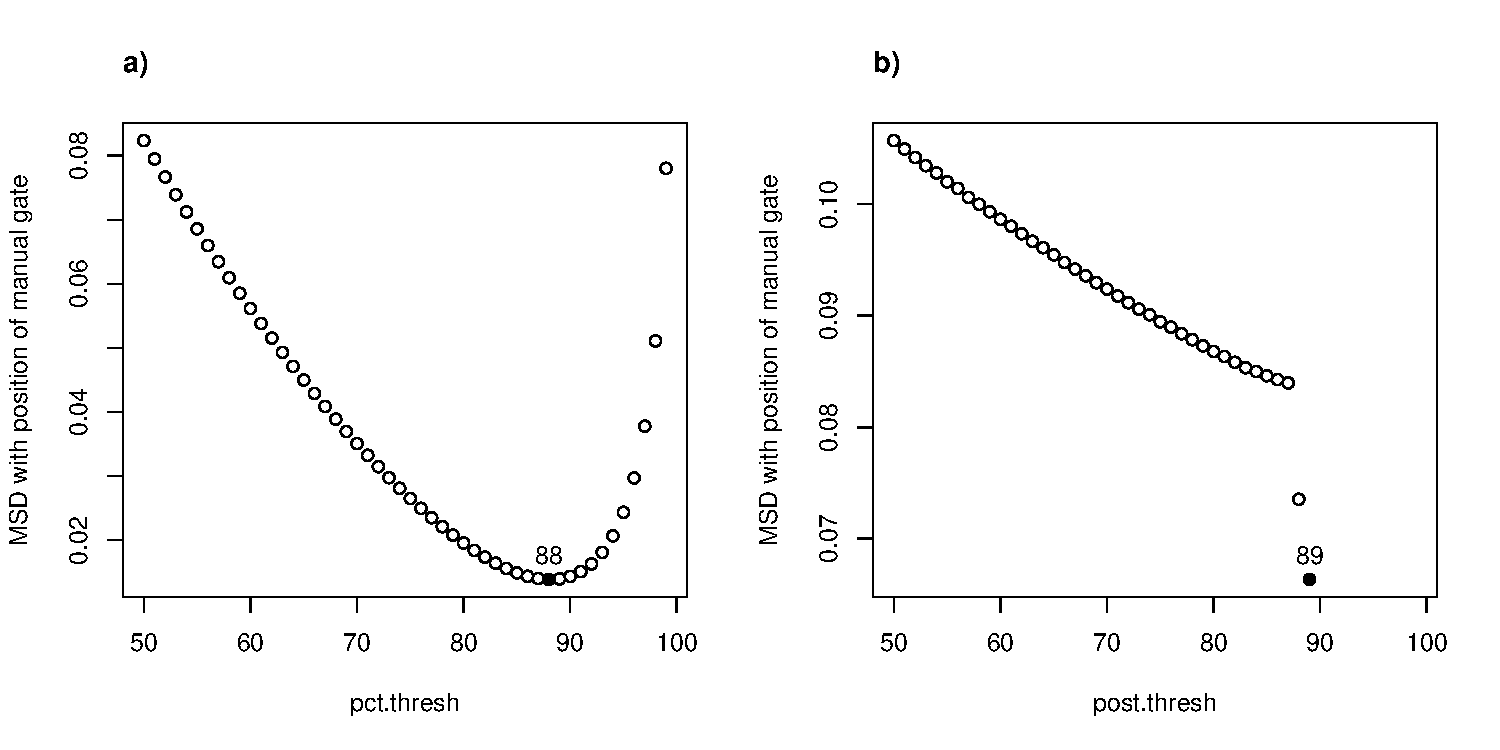
\includegraphics[width=\textwidth]{IL2RA/figures/cd45ra-gate-agreement.pdf}
\mycaption{figure:cd45ra-gate-agreement}
{ Mean square difference (MSD) of the position of the manual gate with that of \texttt{pct.thresh} (a) and \texttt{post.thresh} (b). }
{
  The threshold which minimises the MSD is 88 for \texttt{pct.thresh} (a) and 89 for \texttt{post.thresh}.
  At that threshold, the \texttt{pct.thresh} (a) gate position matches better the manual than \texttt{post.thresh} (b).
  For \texttt{pct.thresh}, the MSD is not defined for threshold larger than 89,
  because there are samples for which the posterior probability does not reach 89 percent (\Cref{figure:cd45ra-posterior-threshold-fail}e).
}
\end{figure}

\begin{figure}[h]
\centering
  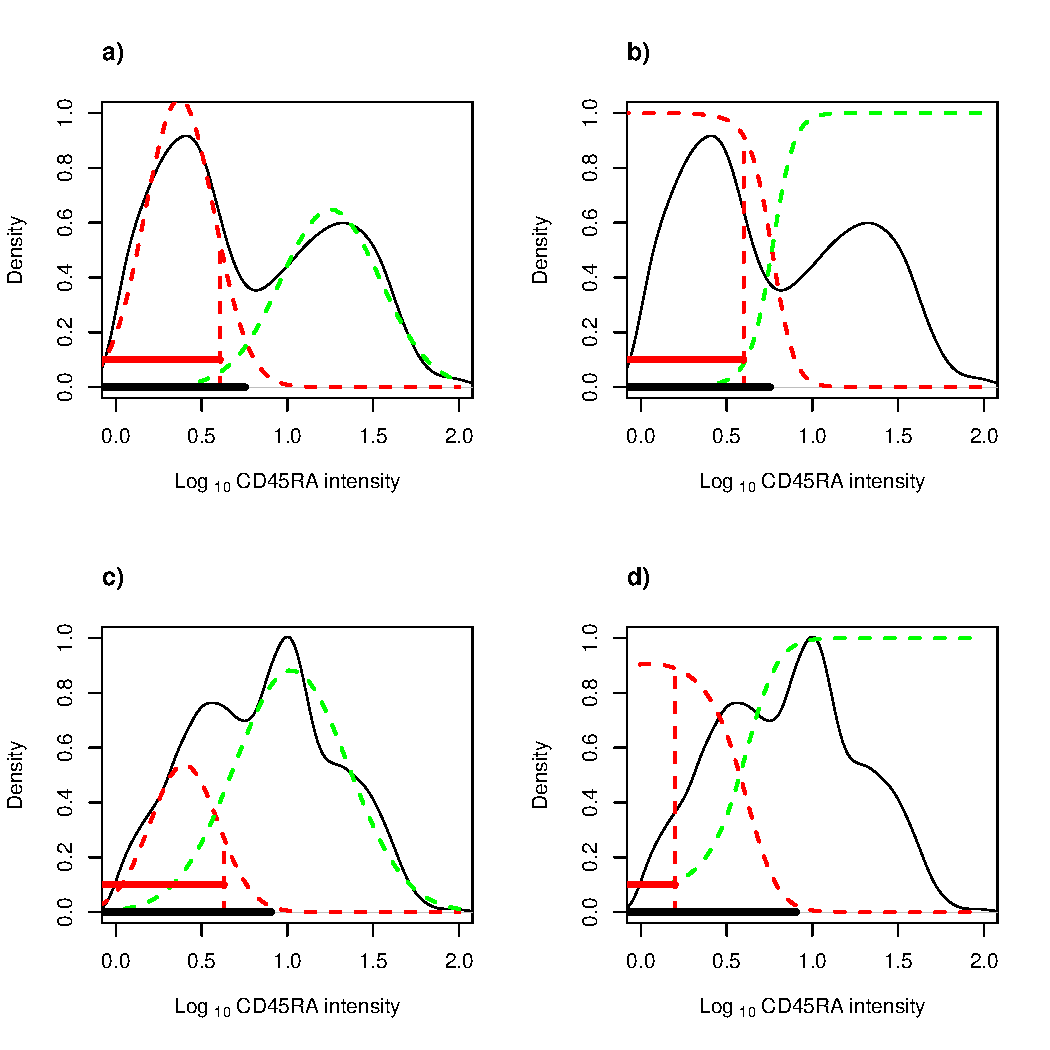
\includegraphics[scale=.6]{IL2RA/figures/cd45ra-threshold-example.pdf}
\mycaption{figure:cd45ra-threshold-example}
{ Example on individual d of the two approaches, \texttt{pct.thresh} (a and c) and \texttt{post.thresh} (b and d), of selecting a threshold. }
{
  Individual d was chosen to illustrate \texttt{pct.thresh} and \texttt{post.thresh}, because
  the CD45RA distribution takes on a very different shape on day one (a and b) compared to day two (c and d).
  In (a) and (c), the \texttt{pct.thresh} method, places the gate at the 88th percentile of the first component.
  In (b) and (d), the \texttt{post.thresh} method, places the gate at the largest CD45RA value where the posterior of the first component reaches 89 percent.
  This poses a problem for \texttt{post.thresh} in (d) because the overlap of the components is such that the posterior is only reached close to zero
  which yields a much smaller gate and consequently a lower percent of memory cells (\Cref{figure:memory-auto-manual-agreement-thresholds}d).
  On the other hand, while the two-component distribution is not a good fit to the data, this is less of an issue for \texttt{pct.thresh}, as can be seen in (c).
}
\end{figure}

\begin{figure}[h]
\centering
  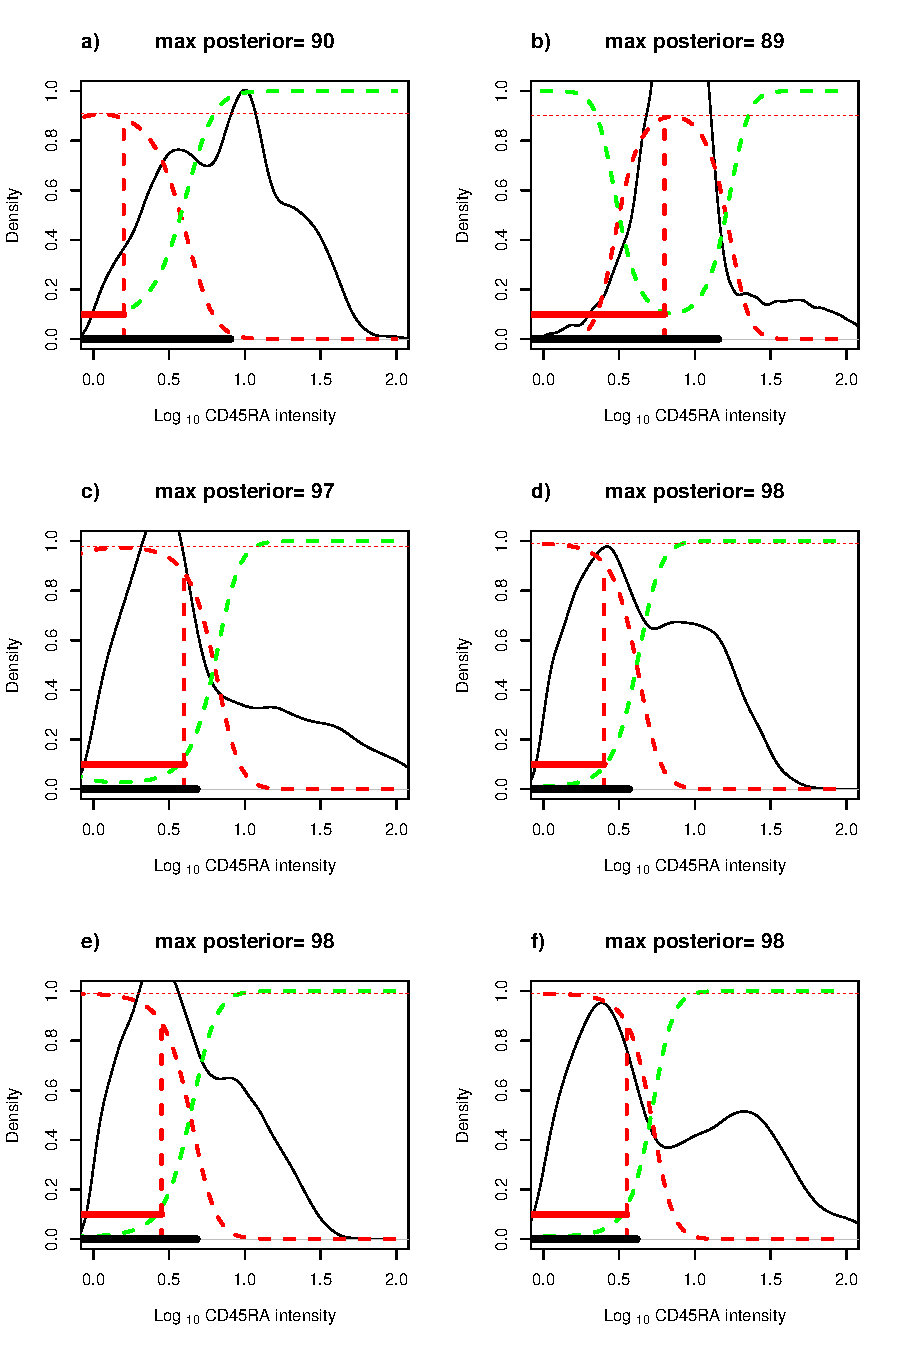
\includegraphics[scale=.6]{IL2RA/figures/cd45ra-posterior-threshold-fail.pdf}
\mycaption{figure:cd45ra-posterior-threshold-fail}
{Samples for which the 99 maximum posterior probability is not reached.}
{
  In black the manual gate.  In red the \texttt{post.thresh} gate drawn at $89$.
  The posterior probability does not reach 99 percent in these six samples.
  In a) this is because of poor model fit.
  In the others b), c) and d), this is due to the mixing of the two distributions.
  In b), the non-uniform decreasing posterior function, can be explained by the green distribution, component 2,
  being much wider than the red distribution.
}
\end{figure}


Using either approach, there is good agreement between the CD25 MEF values obtained for the memory population when gated using either the automated
or the manual approach (\Cref{figure:memory-auto-manual-agreement-thresholds}).
%Using either approach, the agreement with manual gating for the memory CD25 MEF is good (\Cref{figure:memory-auto-manual-agreement-thresholds}).
This is to be expected as this cell phenotype is not very sensitive to the position of the \protein{CD45RA} gate
(\Cref{figure:cd45raneg-memory-cd25mfi}).  
Hence, for this phenotype, this translates to similar repeatability to that obtained with manual gating (\Cref{figure:repeatability-memory-thresholds}).
%and similar effect sizes (\Cref{table:memory-cell-mef-effect}).
On the other hand, the repeatability of the percentage of memory cells is very sensitive to the gate position.


\begin{figure}[h]
 \centering
 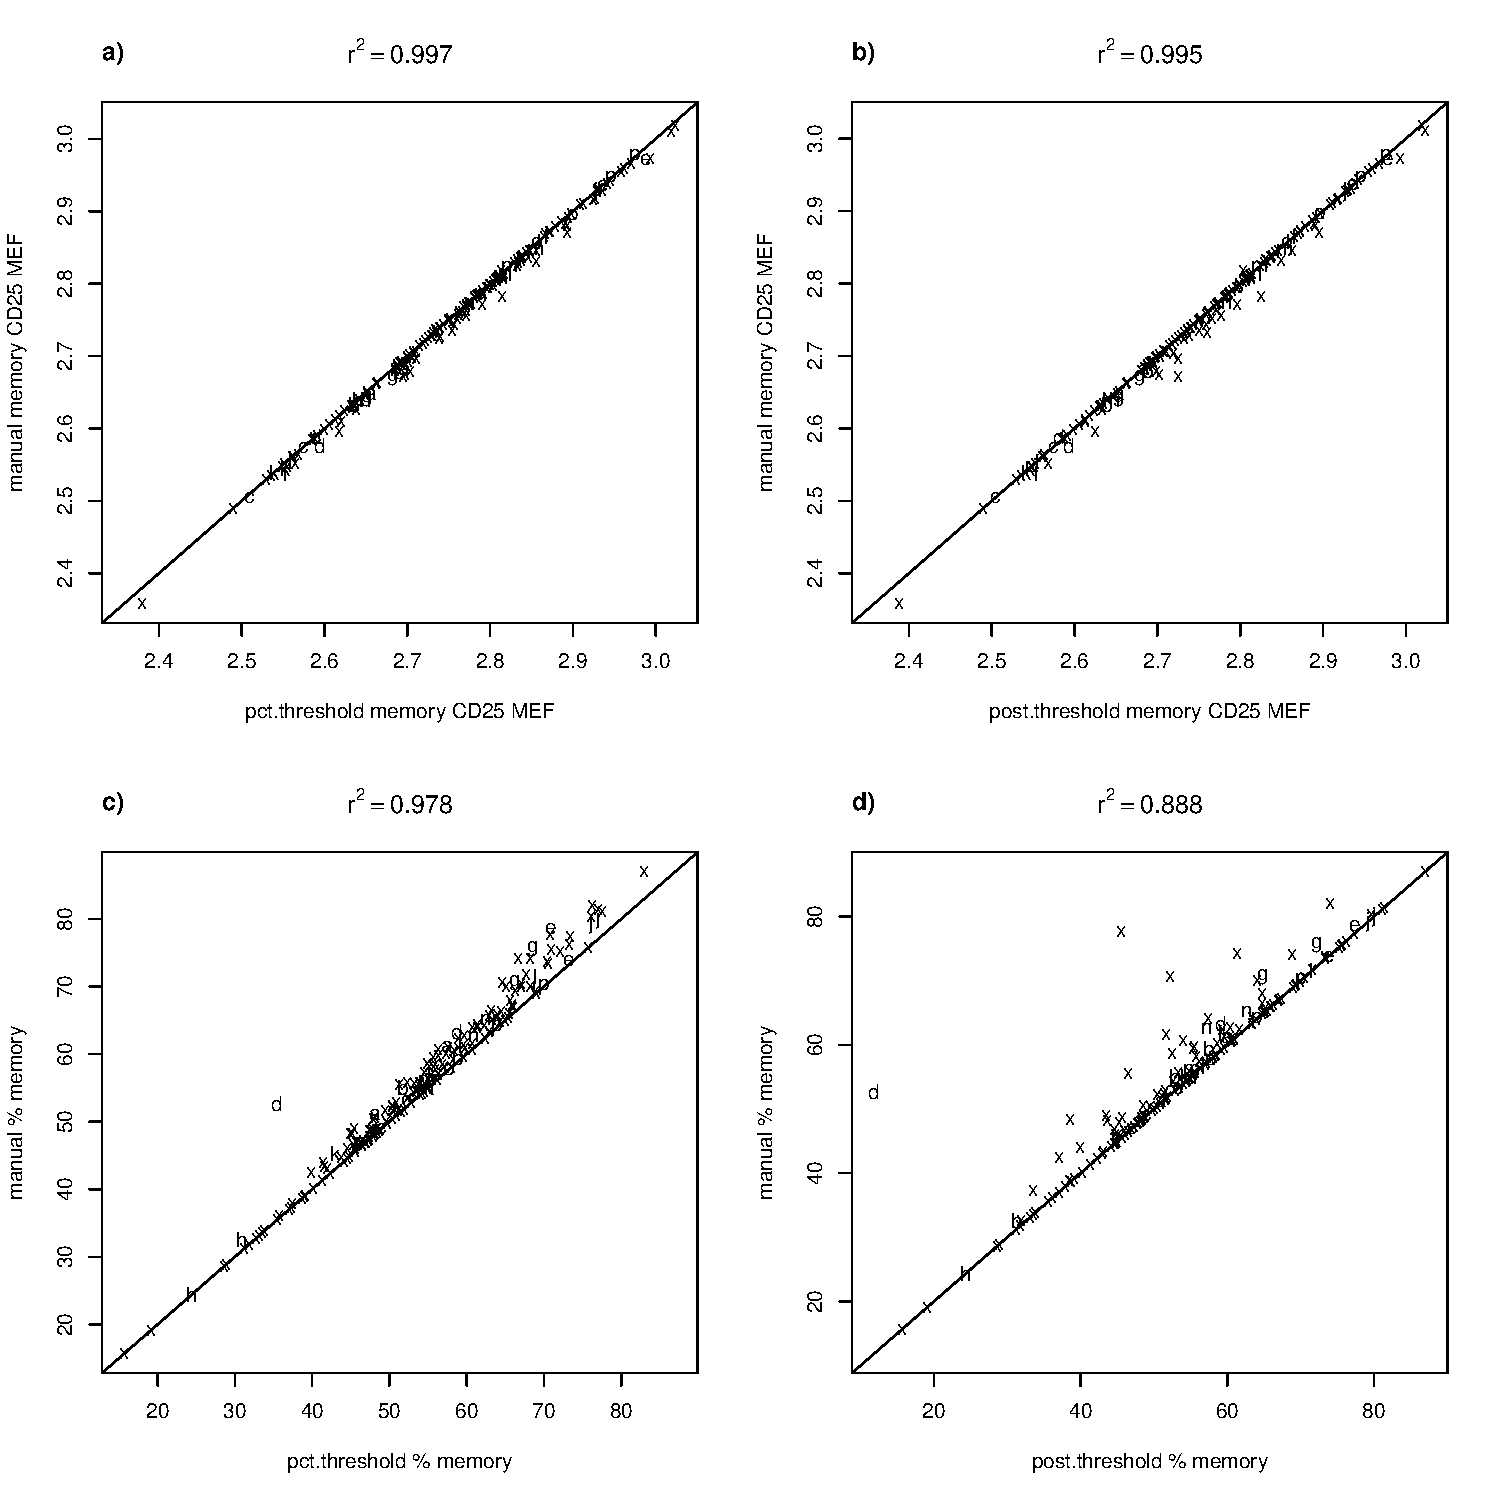
\includegraphics[scale=.6]{IL2RA/figures/memory-auto-manual-agreement-thresholds.pdf}
 %\caption{ Agreement of average daily gate positions of Gaussian mixture model method (day.thresh) with manual for MEF and for memory percentage.}
 \mycaption{figure:memory-auto-manual-agreement-thresholds}
 {Agreement of memory CD25 MEF (a and b) and percentage of memory cells (c and d), obtained from \texttt{pct.thresh} and \texttt{post.thresh} with manual.}
 {
   The agreement of memory CD25 MEF is very close to manual (a and b) while the automatic methods tend to yield smaller memory cell percentages (c and d).
 }
\end{figure} 

%%
\begin{figure}[h]
  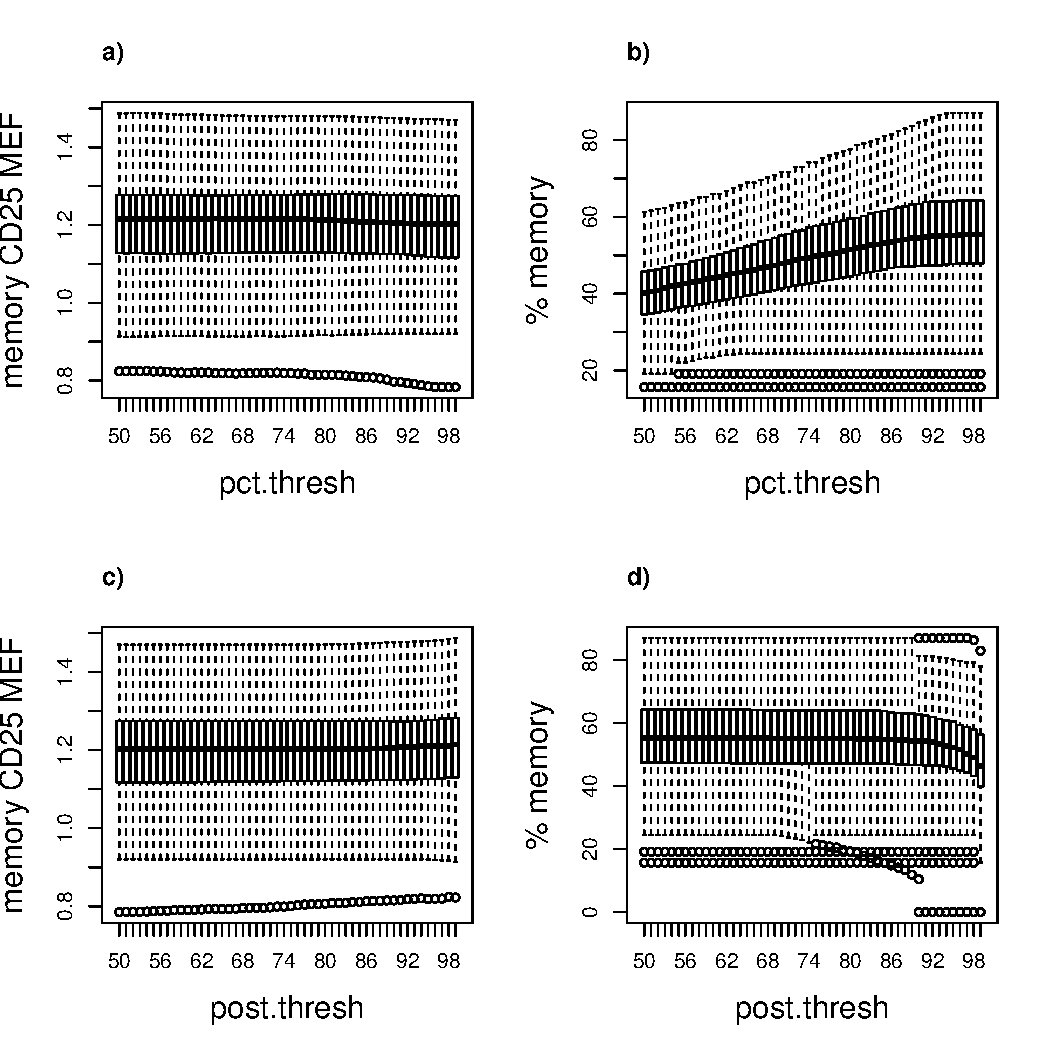
\includegraphics[width=\textwidth]{IL2RA/figures/cd45raneg-memory-gate-phenotype-sensitivity.pdf}
\mycaption{figure:cd45raneg-memory-cd25mfi}
{ Influence of threshold for \texttt{pct.thresh} and \texttt{post.thresh} on distribution of memory CD25 MEF and percent memory cell phenotypes. }
{
  Memory CD25 MEF is not sensitive to position of CD45RA gate (a and c) whereas percent memory is (b and d).
  %The distribution of memory CD25 MEF is not affected by the position of the CD45RA gate.
  On the other hand, the percent memory phenotype is more sensitive in particular when using the \texttt{pct.thresh} (c)
  method as opposed to the \texttt{post.thresh} (d).
}
\end{figure}

\begin{figure}[h]
\centering
  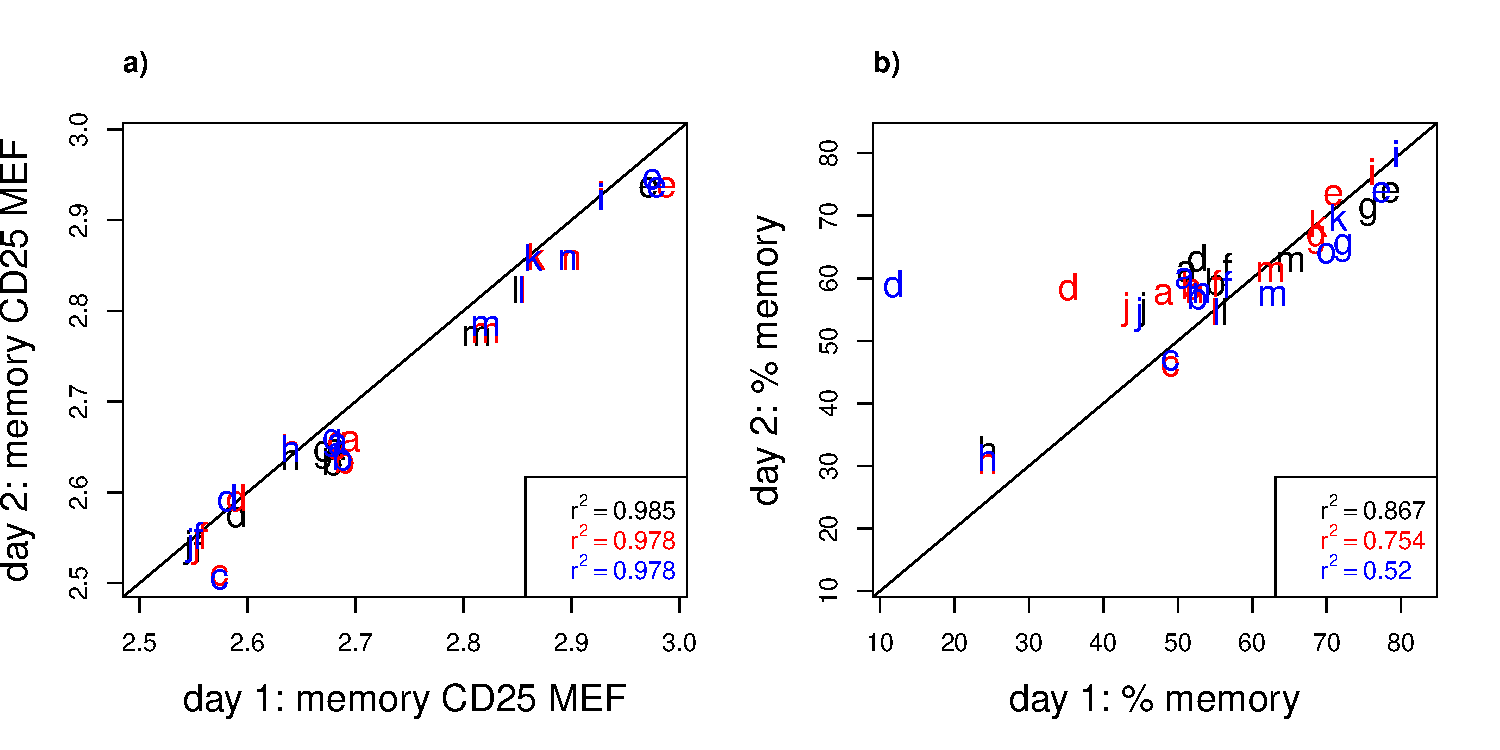
\includegraphics[width=\textwidth]{IL2RA/figures/repeatability-memory-thresholds.pdf}
\mycaption{figure:repeatability-memory-thresholds}
{Repeatability of the memory cells phenotypes, CD25 MEF (a) and percentage (b), obtained from manual gating (black), \texttt{pct.thresh} (red) and \texttt{post.thresh} (blue).}
{
  While the repeatability is very close for CD25 MEF
  ($r^2=0.985$ for manual, $r^2=0.978$ for \texttt{pct.thresh} and $r^2=0.978$ for \texttt{post.thresh})
  it varies considerably for the percentage of memory cells
  ($r^2=0.867$ for manual, $r^2=0.754$ for \texttt{pct.thresh} and $r^2=0.52$ for \texttt{post.thresh}).
  Individual d is a clear outlier when gated with the \texttt{post.thresh} method (b)

}
\end{figure}




\section{Association tests}

Having obtained cell phenotypes by various different gating strategies, 
I would like to assess how these influence our association test statistics.
Since our dataset contains 15 repeated cell phenotypes from recalled individuals,
I accounted for those in my association testing 
by applying a linear mixed effects model with random intercept to allow for per individual effect.
To that purpose I used the \Rfunction{lme} from the \Rpackage{nlme}.
Each covariate, genotype, age and sex, was tested separately, with an additive recessive model assumed for the SNP effect.

Overall, the association test with the percent CD25\positive naive cells phenotype yields similar effect sizes to manual (\Cref{table:naive-cd25pos-association}).
A significant age and \snp{rs2104286} effect are reported using both manual and \texttt{beads.thresh} gating.
However, the significance of the \snp{rs2104286} effect found with \texttt{beads.thresh}, is an order of magnitude less ($10^{-4}$) than with manual ($10^{-5}$).
On the other hand, \texttt{beads.thresh} adds some evidence to the suggested association by \citet{Dendrou:2009dv} of a sex effect on percentage of CD25\positive naive cells,
whereby males have a lower percentage of naive CD25\positive than females, although the effect remains marginal.

Regarding the percentage memory cell phenotype,
an age effect is also detected using automatic methods, \texttt{post.thresh} and \texttt{pct.thresh}, however the signifcance of the association 
is an order of magnitude less with \texttt{post.thresh} (pvalue $10^{-2}$) than with manual and \texttt{pct.thresh} (pvalue $10^{-3}$).
This could be due to greater noise in the measurement as suggested by lower repeatability.
Also, noteworthy, is that a marginally significant \snp{rs2104286} effect (pvalue=$0.042322$) is reported with \texttt{post.thresh}, which is not found with the
other methods.  
However, on closer inspection, the association appears to be driven by the outlying sample from individual d \Cref{figure:rs2104286-memory}.

For the memory CD25 MEF cell phenotype, the association results between manual and automatic are virtually identical (\Cref{table:memory-cell-mef-effect}),
which is to be expected, given this cell phenotype is largely unchanged by the CD45RA gate position (\Cref{figure:cd45raneg-memory-cd25mfi}).

Note that the original results from \citet{Dendrou:2009dv}, which are summarised in \Cref{table:calli-results},
do not match: the repeatability and the p-values are not exactly reproducible.
I believe this is largely due to technical discrepancies between the gating done in FlowJo and the
analysis done in R using the exported FCS and gate files.
However, the analysis I conducted in this chapter is consistent across all samples.



\begin{table}[h]
\centering
\begin{tabular}{lrrr}
\rowcolor{Gray}
\snp{rs12722495} & effect & 95\%CI          & p-value\\
manual           & -2.479  & [-5.422;0.463]  & 0.098145\\
beads.thresh       & -1.509  & [-4.453;1.435]   & 0.31326\\
\rowcolor{Gray}
\snp{rs2104286}  & effect & 95\%CI          & p-value\\
manual           & -4.714  & [-6.894;-2.534]  & \textcolor{red}{3.2017e-05}\\
beads.thresh       & -4.39  & [-6.569;-2.212]   & \textcolor{red}{0.0001014}\\
\rowcolor{Gray}
\snp{rs11594656} & effect & 95\%CI          & p-value\\
manual           & -1.459  & [-3.924;1.006]  & 0.2443\\
beads.thresh       & -1.328  & [-3.774;1.118]   & 0.28531\\
\rowcolor{Gray}
Age              & effect & 95\%CI          & p-value\\
manual           & 0.475  & [0.286;0.664]  & \textcolor{red}{1.6584e-06}\\
beads.thresh       & 0.457  & [0.269;0.645]   & \textcolor{red}{3.514e-06}\\
\rowcolor{Gray}
Sex              & effect & 95\%CI          & p-value\\
manual           & -4.216  & [-7.856;-0.575]  & \textcolor{red}{0.023475}\\
beads.thresh       & -4.327  & [-7.936;-0.718]   & \textcolor{red}{0.019046}\\
\end{tabular}
\mycaption{table:naive-cd25pos-association}
{Genotype, age and sex effect sizes on percentage of \protein{CD25}\positive cells.}
{
Effect of \snp{rs12722495}, \snp{rs2104286}, \snp{rs11594656}, age and sex,
on the percentage of \protein{CD25}\positive naive cells.
}
\end{table}

\begin{table}[h]\footnotesize
\centering
\begin{tabular}{lrrr}
\rowcolor{Gray}
\snp{rs12722495} & effect & 95\%CI         & p-value\\
manual           & 0.062  & [0.036;0.088]  & \textcolor{red}{4.7176e-06}\\
pct.thresh       & 0.06   & [0.034;0.086]  & \textcolor{red}{9.0361e-06}\\
post.thresh      & 0.061  & [0.035;0.087]  & \textcolor{red}{6.822e-06}\\
\rowcolor{Gray}
\snp{rs2104286}  & effect & 95\%CI         & p-value\\
manual           & 0.014  & [-0.007;0.035] & 0.18022\\
pct.thresh       & 0.014  & [-0.007;0.035] & 0.19525\\
post.thresh      & 0.014  & [-0.007;0.035] & 0.18634\\
\rowcolor{Gray}
\snp{rs11594656} & effect & 95\%CI         & p-value\\
manual           & 0.012  & [-0.011;0.035] & 0.29945\\
pct.thresh       & 0.011  & [-0.012;0.034] & 0.34754\\
post.thresh      & 0.011  & [-0.012;0.033] & 0.35147\\
\rowcolor{Gray}
Age              & effect & 95\%CI         & p-value\\
manual           & 0.001  & [-0.001;0.003] & 0.43937\\
pct.thresh       & 0.001  & [-0.001;0.003] & 0.44201\\
post.thresh      & 0.001  & [-0.001;0.003] & 0.38071\\
\rowcolor{Gray}
Sex              & effect & 95\%CI         & p-value\\
manual           & 0      & [-0.034;0.034] & 0.9983\\
pct.thresh       & 0.001  & [-0.033;0.035] & 0.95584\\
post.thresh      & 0.002  & [-0.032;0.036] & 0.89534\\
\end{tabular}
\mycaption{table:memory-cell-mef-effect}
{Memory CD25 MEF effect sizes.}
{
Effect of \snp{rs12722495}, \snp{rs2104286}, \snp{rs11594656}, sex and age on memory CD25 MEF.
}
\end{table}


\begin{table}[h]\footnotesize
\centering
\begin{tabular}{lrrr}
\rowcolor{Gray}
\snp{rs12722495} & effect & 95\%CI         & p-value\\
manual           & 1.736  & [-1.246;4.718] & 0.25209\\
pct.thresh       & 2.326  & [-0.408;5.06]  & 0.094952\\
post.thresh      & 2.624  & [-0.26;5.508]  & 0.074263\\
mm               & 1.131  & [-1.84;4.101]  & 0.45366\\
spmm             & 1.957  & [-1.301;5.214] & 0.23746\\
\rowcolor{Gray}
\snp{rs2104286}  & effect & 95\%CI         & p-value\\
manual           & 1.75   & [-0.544;4.045] & 0.13399\\
pct.thresh       & 2.051  & [-0.063;4.165] & 0.057164\\
post.thresh      & 2.337  & [0.082;4.593]  & \textcolor{red}{0.042322}\\
mm               & 1.118  & [-1.194;3.431] & 0.34129\\
spmm             & 1.775  & [-0.744;4.293] & 0.16611\\
\rowcolor{Gray}
\snp{rs11594656} & effect & 95\%CI         & p-value\\
manual           & -0.018 & [-2.514;2.479] & 0.98884\\
pct.thresh       & 0.269  & [-2.048;2.585] & 0.81927\\
post.thresh      & 0.402  & [-2.092;2.896] & 0.75075\\
mm               & 1.253  & [-1.265;3.771] & 0.32737\\
spmm             & 1.272  & [-1.466;4.01]  & 0.36044\\
\rowcolor{Gray}
Age              & effect & 95\%CI         & p-value\\
manual           & 0.387  & [0.192;0.582]  & \textcolor{red}{0.000127}\\
pct.thresh       & 0.35   & [0.169;0.531]  & \textcolor{red}{0.00018575}\\
post.thresh      & 0.316  & [0.119;0.513]  & \textcolor{red}{0.0018033}\\
mm               & 0.431  & [0.236;0.625]  & \textcolor{red}{2.0985e-05}\\
spmm             & 0.534  & [0.326;0.743]  & \textcolor{red}{1.0325e-06}\\
\rowcolor{Gray}
Sex              & effect & 95\%CI         & p-value\\
manual           & 3.485  & [-0.198;7.168] & 0.063526\\
pct.thresh       & 2.826  & [-0.594;6.246] & 0.10471\\
post.thresh      & 2.811  & [-0.86;6.481]  & 0.1325\\
mm               & 2.793  & [-0.925;6.51]  & 0.13998\\
spmm             & 3.361  & [-0.687;7.408] & 0.10308\\
\end{tabular} 
\mycaption{table:memory-cell-pct-effect}
{Memory percentage effect sizes.}
{
Effect of \snp{rs12722495}, \snp{rs2104286}, \snp{rs11594656}, sex and age on memory cell percentage.
}
\end{table}



\begin{table}[h]\footnotesize
\begin{tabularx} {\linewidth} {|XlcXXX|}
\cline{1-6}
\mbox{CD4\positive T Cell} Subset  & Phenotype  & Repeatability ($r^2$) & Genetic Effect                                                            & Age Effect                                & Sex Effect\\
\cline{1-6}
CD25\positive Naive                & Percentage & $0.669$               & \mbox{$\downarrow$ \snp{rs2104286}} \mbox{$\text{P}=4.25 \times 10^{-6}$} & $\uparrow$ \mbox{$P=2.22 \times 10^{-9}$} & \mbox{M < F} \mbox{$P=0.005$}\\
\cline{1-6}
Memory                     & CD25 MEF   & $0.997$               & \mbox{$\uparrow$ \snp{rs12722495}} \mbox{$\text{P}=1.16 \times 10^{-10}$} & None                                      & None \\
\cline{2-6}
                           & Percentage & $0.862$               & None                                                                      & $\uparrow$ \mbox{$P=8.97 \times 10^{-5}$} & None \\
%CD4\positive FOXP3\positive T Cells
%CD25 MEF
%Percentage
\cline{1-6}
\end{tabularx}
\mycaption{table:calli-results}
{Repeatability and effect sizes of percentage of naive \protein{CD25}\positive \protein{CD25} MEF and percentage of memory cell phenotypes.}
{
Subset of results from \citet{Dendrou:2009dv} for cell populations under re-analysis in this chapter.
$r^2$ is the Pearson correlation squared.
}
\end{table}

\begin{figure}[h]
\centering
\begin{subfigure}[b]{.4\textwidth}
    \centering
    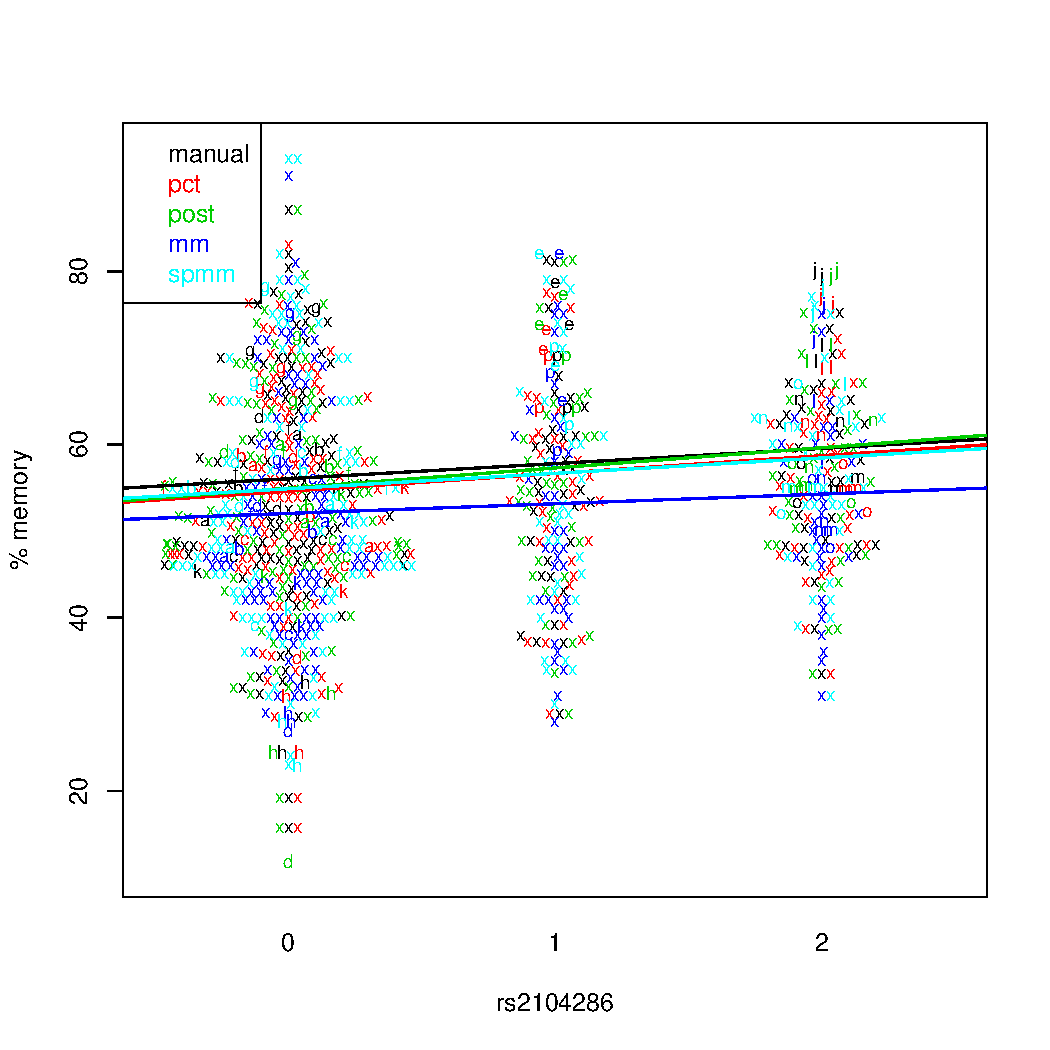
\includegraphics[scale=.35]{IL2RA/figures/rs2104286-ratio.pdf}
    \caption{}
\end{subfigure}
~
\begin{subfigure}[b]{.4\textwidth}
    \centering
    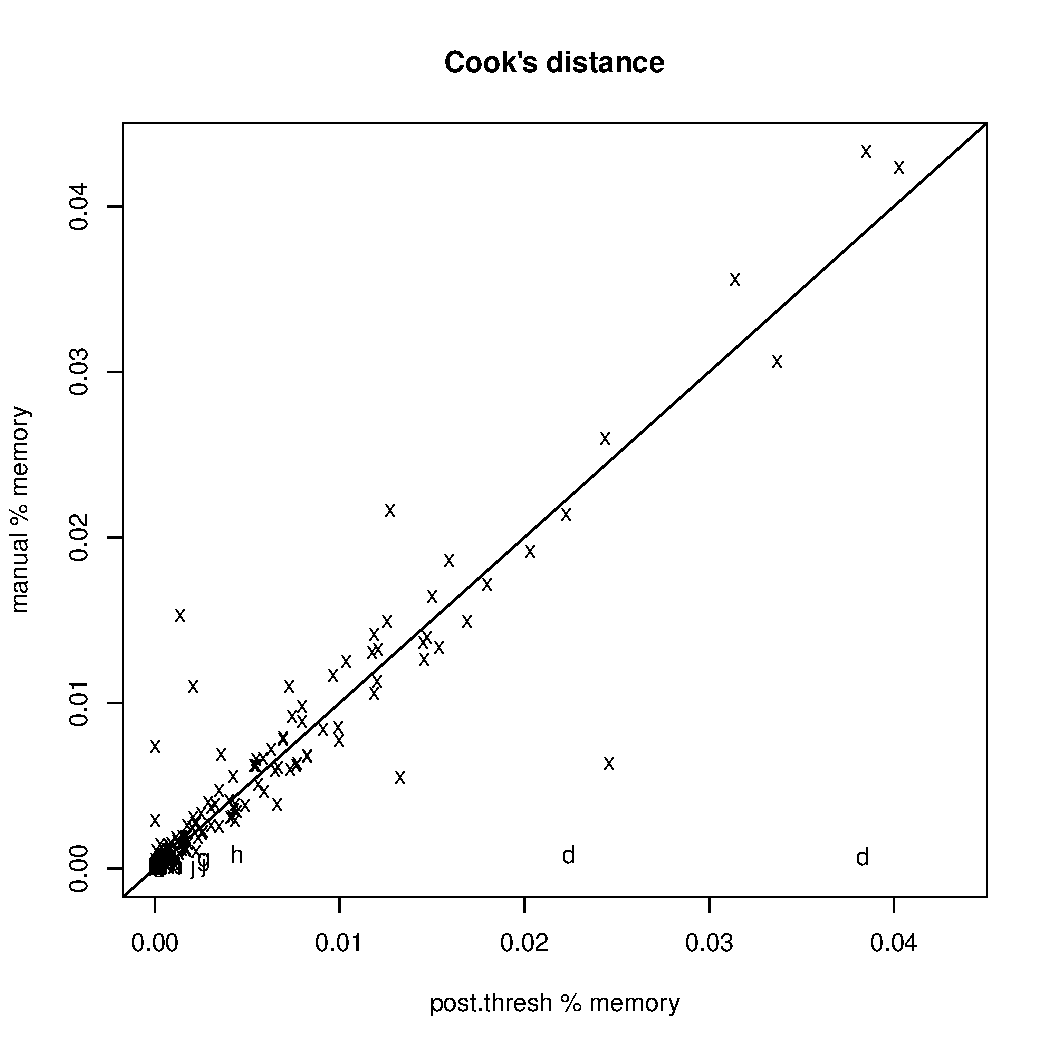
\includegraphics[scale=.35]{IL2RA/figures/rs2104286-ratio-cooks-distance.pdf}
    \caption{}
\end{subfigure}
\mycaption{figure:rs2104286-memory}
{Effect of rs2104286 on percent memory gated by manual (black), \texttt{post.thresh} (green) and \texttt{pct.thresh} (red).}
{
  In \Cref{table:memory-cell-pct-effect}, marginally significant association is detected with \snp{rs2104286}.
  This is due to the leverage of individual d which stands out as an outlier (b).
}
\end{figure}



\clearpage


%%% DISCUSSION
\section{Discussion}

%A more real challenge however is to do with the nature of flow data.
%Noise or unexplained variation is inherent to all technologies and the signal to noise ratio in flow cytometry can vary greatly depending on the sample,
%the experimental protocol and the instrument.
%Even when running a "clean" sample such as beads which are manufactured to be identical on a well calibrated instrument the signal to noise ratio of the resulting bead populations is never greater than 30.
%In biological samples the level of noise is much higher and so is the number of outliers which contribute to confusing automatic methods,
%especially when in most cases the number of clusters is unknown and needs to be estimated from the ratio of explained to unexplained variance in the data.
%Many clustering solutions have been suggested as part of the Bioconductor suite of packages which adopt different approaches to trying to solve this problem.
%But remains the problem of how to benchmark these various solutions: comparison to manual gating, correlation with clinical outcome?
%One criteria we have suggested and tested is that of repeatability of results derived from stable features in samples from the same healthy individual recalled up to 7 months later. (Spidlen et al., 2010).
%
In this chapter, I have shown that bead data is readily gated by automatic methods and that the results are comparable to manual gating.
Automatic gating of bead data is fast and automates other related tasks such as MFI to MEF transformation, and threshold selection.
%and reporting of instrument properties such as the detection threshold or the signal-to-noise ratio (or coefficient of variation).

Gating of biological data is more difficult as we have little prior knowledge of the sample we are analysing.
So far, I have developed two automatic univariate gating strategies:
\begin{itemise}
\item a bead defined threshold method on \protein{CD25} to identify CD25\positive naive cells
\item a two component mixture model on \protein{CD45RA} to identify memory cells (CD45RA-)
\end{itemise}

My \protein{CD25} univariate gating method (\texttt{beads.thresh}) relies on defining a threshold based on automatically gated bead data.
The value of the threshold is selected as the percentile of the blank bead population which mimimises the mean squared difference with manual gate positions.
The percentage of naive \protein{CD25}\positive cells phenotype identified with my approach showed better repeatability than manual (\Cref{figure:repeatability-cd25pos-naive}).
My approach defines one threshold for all samples gated on the same day,
%which seems appropriate given the blank bead population yields the detection threshold of the instrument on that day.
whereas the manual approach, relies on isotype controls and allows for different thresholds per day.
Isotype controls should theoretically be an estimate of background but have been criticised for being an extra source of noise \citep{OGorman:1999vd}.

My \protein{CD45RA} univariate gating method fits a specific model to the data: a mixture of two univariate distributions.
The parameters of the model are estimated using an \Gls{EM} algorithm \citep{Dempster:1977ul} initialised with K-medoids (\Cref{appendix:clustering}).

In a first instance, I used the parameters estimated by the two-component mixture model.
Specifically, I used the weight parameter of the first component as the percentage of memory cells phenotype.
%Additionally to the mixture of two univariate Gaussian model (\texttt{mm}), I also applied a more flexible model of two symmetric kernel density estimates (\texttt{spmm}).
Although this seemed a sensible approach from the statistical perspective of fitting a two-component mixture model, it does not match the biological perspective that cells transitional cells should be excluded.



Therefore, in the second instance, I attempted to emulate manual gating by defining a threshold.
I tried two approaches of defining a threshold, \texttt{pct.thresh} which thresholds on the percentile of the first component of the fitted mixture model,
and \texttt{post.thresh} which thresholds instead on the posterior probability of the first component.
As with the \texttt{beads.thresh}, the value of the threshold is selected as the value which mimimises the mean squared difference with manual gate positions.
%In the future it may be interesting to use all cells and average over the posterior probabilities.
%I have found however that there is sometimes an upper bound to the posterior probability
%However, if the model does not fit the data then it is unlikely that the position of the gate will be sensible, which may give rise to outliers.

Two benchmarks were used to evaluate my univariate gating strategies: repeatability and comparison of the effects sizes obtained 
by \citet{Dendrou:2009dv} using manual.

Repeatability is an independent measure which does not require comparison to other gating methods (such as manual).
Unfortunately, given that in our data set only 15 samples are repeated, it is difficult to evaluate methods on such a small sample size.
Moreover, good repeatability does not necessarily imply that the gating is unbiased but rather that the gating is consistent.
Hence repeatability, needs to be complemented with some metric, in the form of manual gating or some prior biological knowledge,
to assess whether the computed cell phenotypes are in a sensible range.

I have shown that the difference in the identification of cell phenotypes by different gating methods can influence the effect size estimates in association studies.
In particular, outliers can have an important influence in relation to their leverage as seen in \Cref{figure:rs2104286-ratio}.
For example when testing association with age, outlier cell phenotypes from younger or older individuals have more leverage than ones closer to the mean.
When testing for association with genotype, outlier cell phenotypes from rarer variants have more leverage than one from common variants.

%\paragraph{Outlier Detection Metric}
Hence, if we are to deploy automatic gating techniques more generally, detection of outliers is crucial, to avoid false positive associations.
In particular, we require outlier detection metrics which do not only rely on the availability of repeated samples or manual gates.
Already, we have seen that looking at the maximum posterior probability in a sample can give us some insight (\Cref{figure:cd45ra-posterior-threshold-fail}).
Another metric of evaluating how well a model fits the data could be a cost function like the Mean Integrated Squared Error (MISE).
I will expound on other outlier metrics in later chapters.

When outliers have been detected, we may want to exclude or down-weight them, or extend our gating method to account for these.
One simple way of modifying the method, could be to use the gate positions in non-outlier samples to influence those in outliers.
This motivates borrowing information from other samples, using for example a hierarchical Bayesian framework as was recently developed by \citet{Cron:2013dh}.

However, one may argue that this approach, conceals rather than addresses the underlying problem of poor model fit.
For example, as we see from the trimodal distribution in \Cref{figure:cd45ra-threshold-example},
it may be more appropriate to fit a three component instead of a two component mixture model on this sample.

So far, MFI to MEF using beads has been automated but there are still many parts of the process which can be automated.
In later chapters, I will develop a modular pipeline to further automate the analysis of flow cytometry data generated by our lab.
It will be possible to plug in different types of transformations and gating strategies and see how this influences
the results of the analysis.
This should encourage the wider use of automatic analysis methods for flow data within our lab.

Chris points:
Manual gating could be applied in a subset of samples and then auto gating could use that info to guide the gating.
This provides reassurance to gaters that their rules are follow.  Manual gaters may not always be keen to relinquish control
to a computer: seeing is believing.


%\paragraph{Discovering New Subsets of Interest with Automatic Methods}
%So far in this chapter, I have only considered the cell phenotypes defined by \citet{Dendrou:2009dv}.
%In general, these cell populations may not necessarily represent true clusters but are established cells of interest within the field of immunology
%which are known to express \protein{CD25} and hence hypothesised to associate with \gene{IL2RA} SNPs.
%Potentially, there might exist other \protein{CD25} cell phenotypes than the ones under study which also correlate well with these SNPs.
%These might only be separable in higher dimensional space.
%These could be identifiable using unsupervised methods which find clusters in one or more dimensions when the number of clusters is unknown.
%Similar work has been undertaken by \citet{Aghaeepour:2012fq} in identifiying novel subsets which correlate with a clinical outcome in HIV patients.
%Fealect (?) is a method of choosing features of these cells subsets which best correlate with the response variable.

%\paragraph{An Internal Automatic Pipeline}


%The pipeline will be configurable to so account for the wealth Obviously the type of analysis will be dependent on the experiment but it may be possible 
%One of the reasons for this is simply that the analysis requirements for different types of flow experiments are so varied that it is difficult to design a solution which will service all needs.


%% TODO
%This clearly rests on the assumption that in the majority of samples, the position of the gate is correct.
%I tried this approach with \texttt{day.thresh} by averaging gates on non-outlier samples and applying these to the outlier samples.
%thus exploiting day effects
%A more formal approach could be to extend this by using some outlier metric to define weights so that \texttt{day.thresh} leans more heavily
%towards samples where the model fits better.
%We have seen that one way of improving overall gating is to allow for the gate positions on well-gated samples to influence those of badly-gated ones.
%Clearly, the implicit assumption with \texttt{day.thresh} and outlier detection in general, is that there are enough well-gated samples to positively influence the gate position of the ill-gated ones
%and that the gates in outlier samples should be in about the same position since the sample is noisy but not fundamentally different.  
%One reason why the manual gates on that day are more appropriate is because a human uses prior knowledge obtained from other samples of where the gates should lie.
%A first attempt at learning from other samples (\texttt{day.thresh}) is to compute the mean of the position of the CD45RA gates defined by the \texttt{pct.thresh}
%method across all samples from the same day excluding the outlying sample from individual d on day one.
%Similar to the threshold method for \protein{CD25}\positive covered in the previous section, we now have a fixed gate for all samples analysed on the same day.
%The \texttt{day.thresh} agreement with manual is improved over x but not as good as y
%%but this time requires estimation of gate position by mm followed by averaging their position.
%%When attempting to gate more noisy samples, a manual gater will maybe use other samples as a reference.
%%One way of better gating is to use prior knowledge from other samples from the same day where the repeatability is good.
%Since the gate position is less sensitive to outlier samples, \texttt{day.thresh} improves overall repeatability (\Cref{figure:repeatability-memory-thresholds-learned}) compared to \texttt{pct.thresh}.  
%Nonetheless, manual still achieves higher repeatability (\Cref{table:repeatability-results}) as
%the gater has prior knowledge of cell population frequencies when dealing with outliers.
%



\clearpage

% Chapter
\chapter{ \label{chapter:il2} Methods to assess cell response to ex-vivo stimulation in flow cytometry }
%\chapter{ \label{chapter:il2} Effect of IL-2 Stimulation on Cell Phenotypes } 
%\chapter{ \label{chapter:il2} A recursive partitioning approach of identifying cells responsive to ex-vivo stimulation in flow cytometry }

In the previous chapter, we looked at normalisation of the MFI using beads and replicating two univariate gating steps with thresholding on CD25
or with a mixture of two components on CD45RA.
Here on a different dataset on which only preliminary manual analysis has been done, we will also consider normalisation methods and replicating all steps of the manual gating
with an automatic procedure.
Furthermore, we will also consider automatic approaches for discovering biologically relevant subsets not reported by the manual gating.

\section{Background}

\paragraph{Motivation}
%\Acrfull{GWAS}
Genomewide association studies have implicated the \cytokine{IL-2} signalling as an important aetiological pathway associated with the development of \gls{T1D}.  
%So far associated regions have been reported close to IL2RA and PTPN2, a phosphatase, which both influence STAT5 transduction.
%The protective rs12722495 haplotype was significantly associated with increase in CD25 expression on CD4 memory T cells measured in terms of MFI.
%Howevever the protective combined rs2104286 genotype led to a decrease in the percentage of CD25 positive CD4 naive T cells.  
As seen in \Cref{chapter:il2ra}, the protective T1D associated \gene{IL2RA} variant at \snp{rs12722495} in healthy individuals predicts an increase in expression of \protein{CD25},
the alpha chain of the trimeric \protein{IL-2} receptor, on memory \protein{CD4}\positive T lymphocytes \citep{Dendrou:2008gc,Dendrou:2009dv}.
%and high levels of IL-2 secretion by these cells
%As supported by an increase in soluble CD25, this might be the consequence of preferential cleavage of the CD25 receptor \citet{Lowe:2007ij}.
%As supported by a decerase in soluble CD25 \citet{Lowe:2007ij}.
\citet{Garg:2012jr} found that regulatory and memory \protein{CD4}\positive T cells in healthy carriers of T1D risk associated \gene{IL2RA} variants,
also exhibit decreased sensitivity to \cytokine{IL-2} in terms of decreased MFI levels of
phosphorylated signal transducer and activator of transcription 5 protein (p\protein{STAT5}),
STAT5 dimerises or tetramerises on phosphorylation and acts as
a transcription factor (\Cref{figure:jones-2000}),
which also induces the transcription of \gene{FOXP3}, a transcription factor characteristic of regulatory T cells .

\begin{figure}[h]
\centering
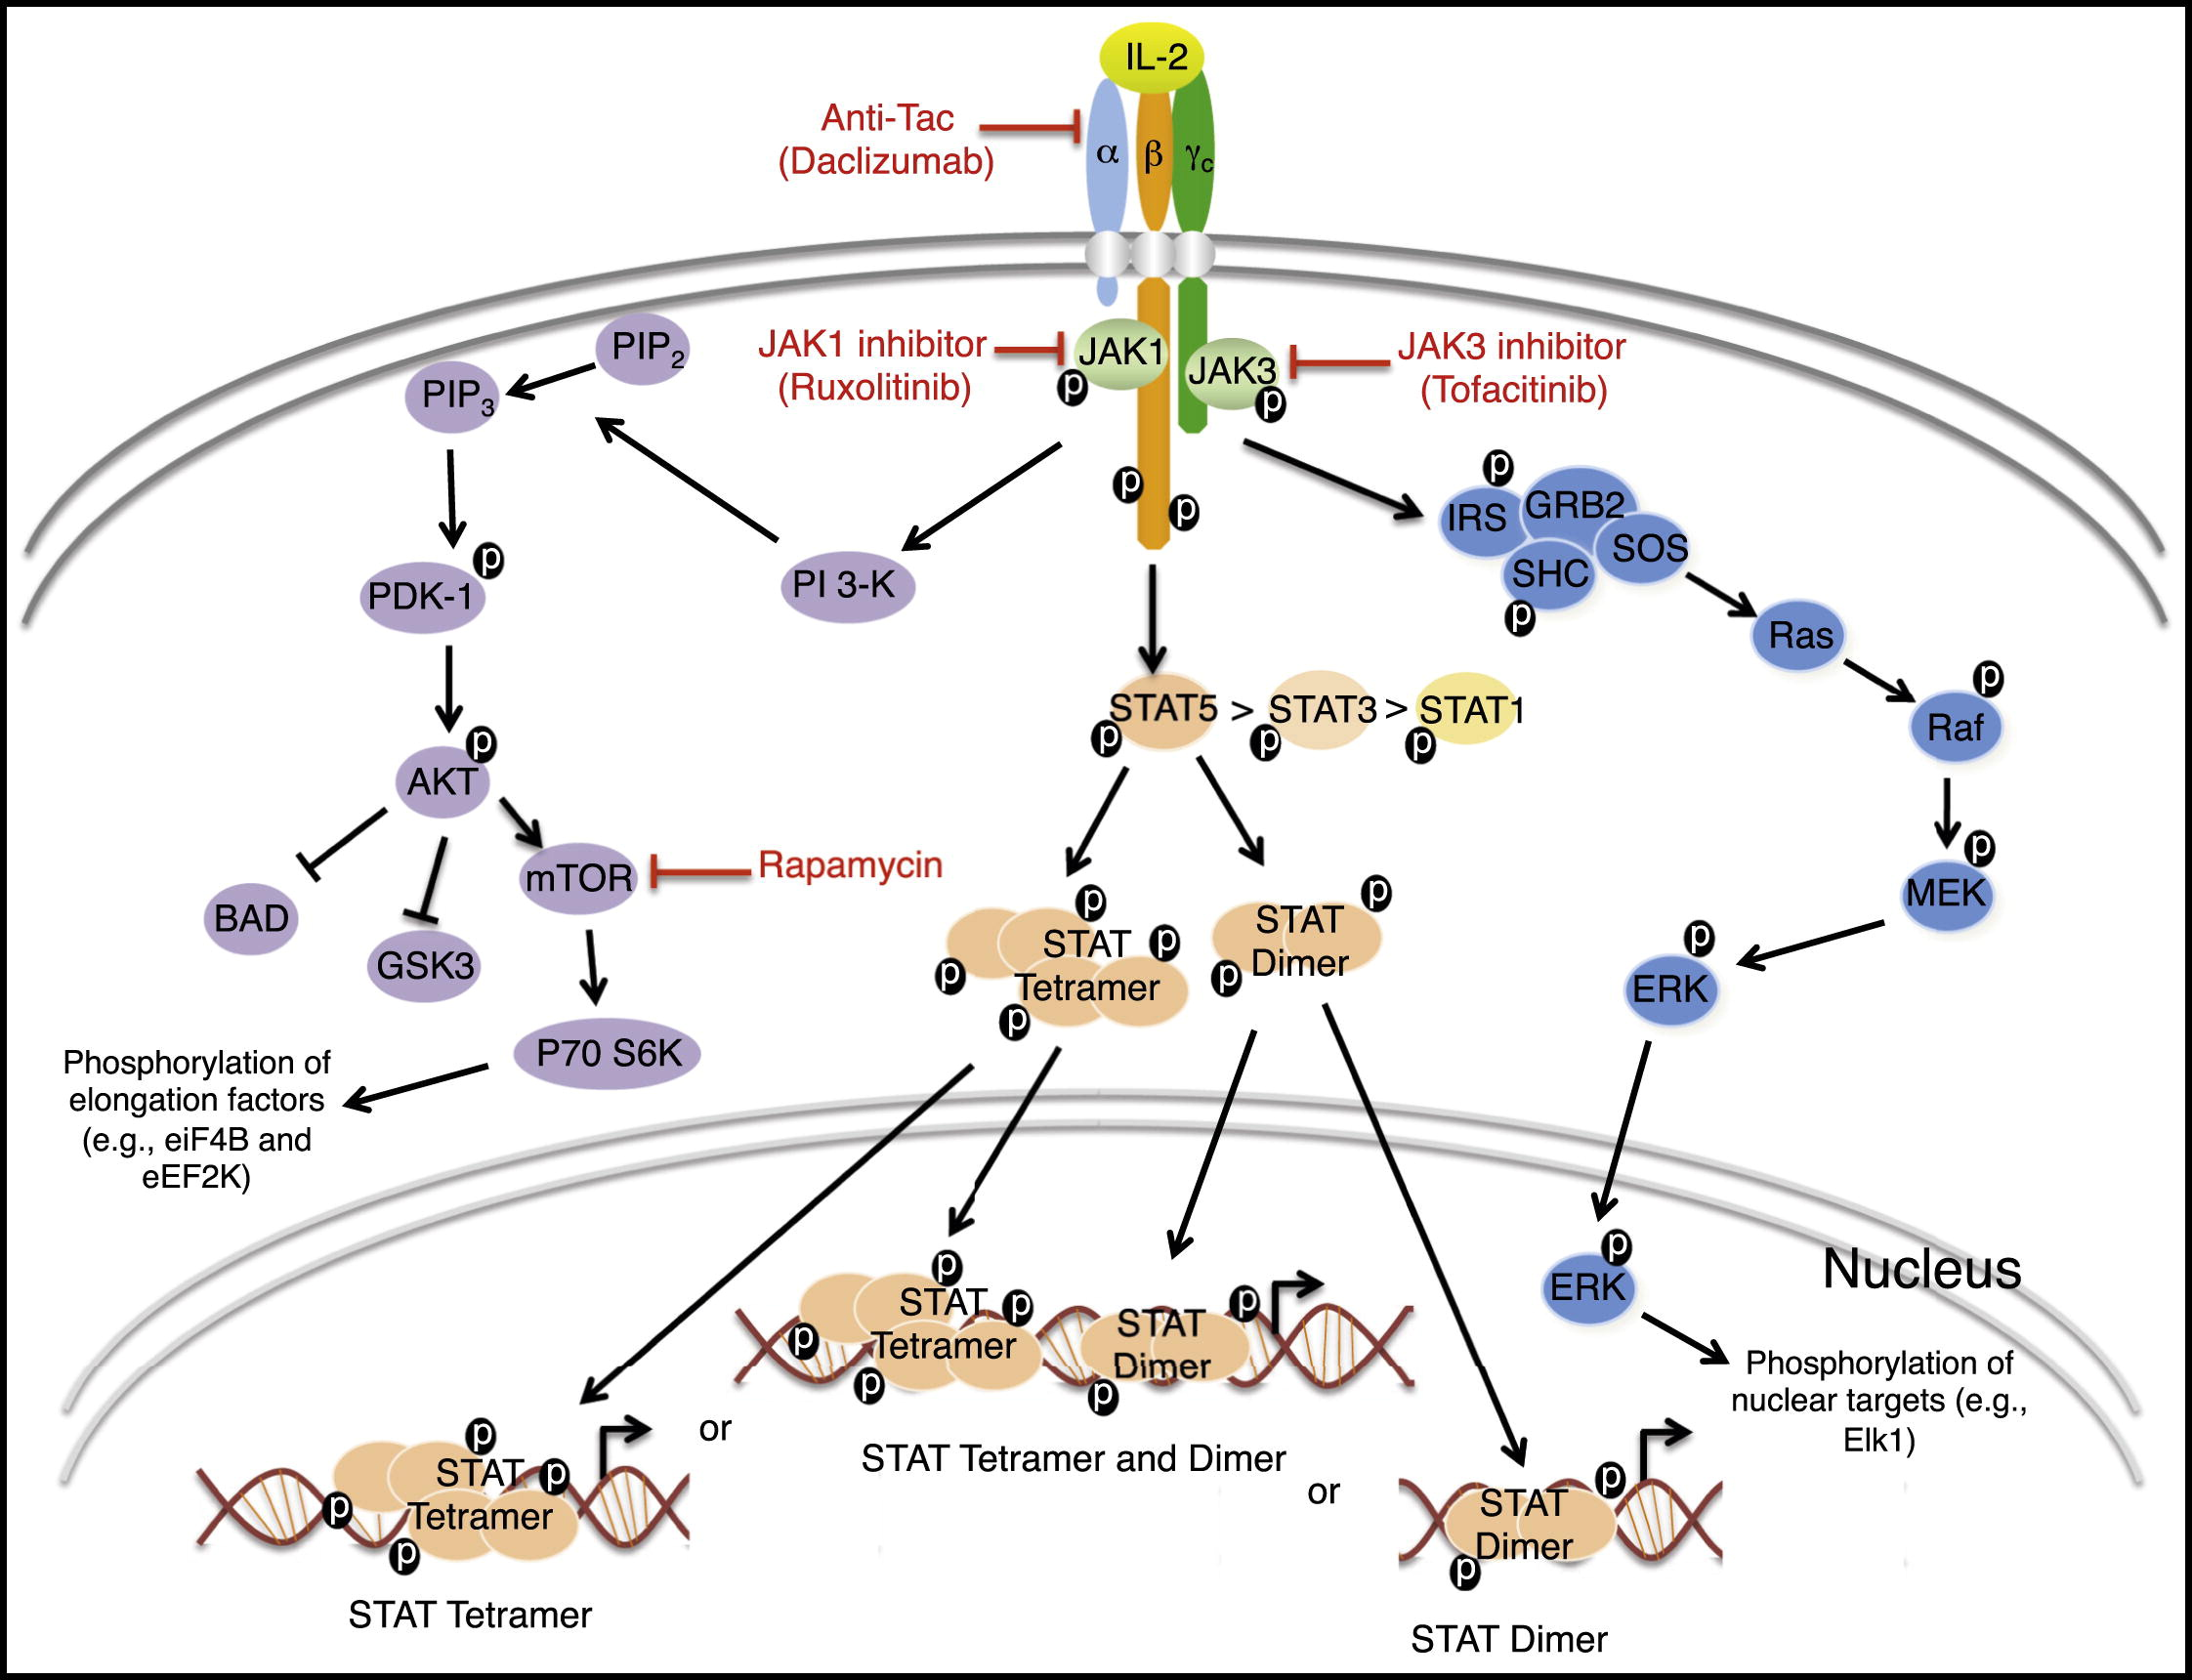
\includegraphics[scale=0.75]{IL2/figures/IL2-pathway.jpg}
\mycaption{figure:jones-2000}
{Schematic of major IL-2 signaling pathway (taken from \citet{Liao:2013jt}).}
{
\protein{CD25} is \protein{IL2RA}, the $\alpha$ subunit of the trimeric \cytokine{IL-2} receptor.
The $\alpha$ chain is the highest binding affinity receptor of the three chains.
STAT5 is phosphorylated to pSTAT5 and acts as a transcription factor.
%Schematic of Major IL-2 Signaling Pathways
%Shown is the activation of PI 3-K-AKT, JAK-STAT, and SHC-RAS-MAPK signaling pathways. Also shown are potential therapeutic points of control for IL-2 signaling, with anti-Tac (daclizumab), rapamycin, and JAK1 or JAK3 inhibitors being shown in red. The cartoon shows signaling by both STATs dimers and tetramers. The figure indicates that IL-2 activates more STAT5 than STAT3 and more STAT3 than STAT1. ERK refers to both ERK1 and ERK2. MEK refers to both MEK1 and MEK2.
}
\end{figure}

\citet{Long:2011hk} have reported that a \Gls{T1D} associated variant at \snp{rs1893217}
of the protein tyrosine phosphatase N2 gene (\gene{PTPN2}),
a negative regulator of the IL-2 pathway,
also correlates with lower STAT5 phosphorylation.
%show diminished ability to respond to \cytokine{IL-2}.
Furthermore, it is suspected that \cytokine{IL-2} production might be diminished in T1D since disease associated \gene{IL2RA} variants 
correlate with reduced CD25 levels 
and reduced \cytokine{IL-2} production
on activated CD69\positive CD4\positive memory T cells
after antigen stimulation \citep{Dendrou:2009dv}.
%with staphylococcal enterotoxin B 
%really?
Long-term reduced sensitivity to IL-2 also correlates with dimished maintenance 
of FOXP3 expression in the CD4\positive CD25\positive regulatory T-cells of type 1 diabetic subjects \citep{Long:2010ej}.
%Defects in IL-2R signaling contribute to diminished maintenance 
%IL-2 sensitivity drives IL-2 stimulation
%Preliminary data also suggests that the sensitivity to IL-2, measured in terms of pSTAT5 activation, may be also be reduced in the regulatory CD4+ T cells of newly diagnosed T1D patients.
%Furthermore it is also suspected that IL-2 production might be diminished in T1D
%since disease associated variants in the \emph{IL2RA} and \emph{PTPN2} genotypes correlate with reduced IL-2 production (reference?). 
Hence, these findings appear to consolidate the hypothesis that type 1 diabetics tend to have a reduced ability to respond to IL-2
in part due to genetic defects in \gene{PTPN2}, \gene{IL2RA} and possibly other gene variants involved in the IL-2 signalling pathway
%and that this decreased sensitivity is most noticeable in regulatory T cells
\citep{Long:2010ej,Long:2011hk,Long:2012ea}.
%The cell subsets are not always consistently defined across studies.
%Long:2010ej define Tregs as CD4+ CD25hi (FOXP3 not measured)
%Long:2011hk report that CD4+ CD45RO+
%nor is the definition of response to IL-2
%sometimes pSTAT5 MFI is measured, sometimes pSTAT5 pct positive, sometimes pSTAT5 fold change
These results are of great clinical relevance to us,
since our lab is currently conducting an
adaptive study of IL-2 dose on regulatory T cells in type 1 diabetes (\url{http://www.clinical-trials-type1-diabetes.com/}),
and to all researchers interested in low-dose IL-2 therapy to autoimmune diseases \citep{Koreth:2011kv,Saadoun:2011em}.

However some concerns have been raised with these studies.
One concern was that the Tregs discrimination was not particulary thorough.
%nor consistent
\citet{Long:2010ej} define Tregs based only on two markers CD4\positive CD25\positive whereas these cells are usually
also defined on CD127 and FOXP3.
Another a notable omission by \citet{Long:2010ej} was the lack of repeated samples to assess the within-individual variance
or reliability of the assay.
%Although \citet{Long:2011hk} do assess repeatability in 16 individuals, its not accounted for in the association test.
%clinical trials which
%treat type 1 diabetics with IL-2.
Hence, \contributor{Tony Cutler}, in our lab, set to find if he could replicate some of these findings in an independent cohort
using a more refined gating stategy by including the FOXP3 regulatory T cell marker,
%T1D leads to decrease sensitivity to IL-2 in similar sample size with 
as well as NK cell markers, CD3, CD8, and CD56,
%and the naive cell marker CD31,
to discover whether other potential cell subsets
are also sensitive to IL-2 (\Cref{table:IL2-panels}).
%and using repeated samples.

\paragraph{Samples and panels}

He selected 22 long-standing diabetics (6 males and 16 females, mean age 29) and 28 controls (mean age 27) from the Cambridge Bioresource,
as well as 30 newly diagnosed (20 males and 9 females, mean age 11.7) and 15 unaffected siblings (5 males and 12 females, mean age 12.3) from the \Gls{D-GAP} resource.  
%This was to determine if there was a difference between newly diagnosed and long-standing diabetics while controlling for age.
To guard from false positive association and non-reproducible results, 
it is important to ascertain the repeatability of these cell phenotypes before conducting any form of association study.
%Before proceeding with association testing of these cell phenotypes with T1D status or other covariates,
In order to test the repeatability, ten individuals were recalled for a second blood sample (\Cref{table:IL2-recalled-individuals}).
Hence a total of 52 cases and 43 controls, of which, 10 individuals (5 cases and 5 controls) from the Cambridge Bioresource were recalled to assess reproducibility
of the phenotypes.  

\begin{table}[ht]
\centering
\begin{tabular}{llll}
  \hline
Individual & status  & pch & number of days between visits \\
  \hline
1          & control & a   & 98 \\
2          & case    & b   & 140 \\
3          & control & c   & 167 \\
4          & control & d   & 98 \\
5          & case    & e   & 167 \\
6          & case    & f   & 112 \\
7          & control & g   & 112 \\
8          & case    & h   & 98 \\
9          & case    & i   & 120 \\
10         & control & j   & 140 \\
   \hline
\end{tabular}
\mycaption{table:IL2-recalled-individuals}
{Ten individuals recalled between 98 and 168 days later to assess stability of the cell phenotypes. }
{
pch is the plotting character used to refer to these individuals in plots later in this chapter.
}
\end{table}
%In order to test these hypotheses, we selected 21 long-standing diabetics and 30 controls from the Cambridge Bioresource,
%as well as  28 newly diagnosed and 14 unaffected siblings from DGAP.
%The nature of the resource allows more flexibility to recall patients of interest, i.e those with low IL-2 signalling potential, for more in depth analysis.
%To test this hypothesis, blood samples are taken from 21 type 1 diabetics and 30 healthy controls.  
Blood samples were prepared and analysed by flow cytometry on day of collection.
Each sample was split into four aliquots of \SI{500}{\micro\litre}.
The first aliquot was left unstimulated.
The remaining three were stimulated ex-vivo for 30 minutes at four 100-fold increasing doses
of proleukin (a polymer of \cytokine{IL-2}) at $0.1$, $10$ and \SI{1000}{\unit\per\milli\litre} respectively.
%\SI{1000}{\unit\per\micro\litre} respectively.
After a set stimulation time, the samples were fixed, permeabilised and stained, with different panels (\Cref{table:IL2-panels}), 
on a set of core markers, not expected to be affected by short-term proleukin stimulation,
CD4, CD25, CD45RA and FOXP3.
These were used to delineate different cell types, and the functional marker, pSTAT5
, a signalling protein of the IL-2 pathway phosphorylated on IL-2 stimulation (\Cref{figure:jones-2000}),
was used to measure IL-2 response.
Samples were analysed individually with flow cytometry, with all \gls{T1D} samples except for two run in parallel with healthy controls
to account for batch effects (\Cref{figure:IL2-sample-time}).
Samples were also matched for age and sex to allow for paired analysis.

%We address the following research questions relating to the pSTAT5 response in these samples:
%\begin{itemise}
  %%\item Can some individuals be classified as low/high responders?
  %\item In the cell subsets identified by manual gating, is the response to IL-2 associated with case-control status or any other covariate? 
  %\item Using automated methods, can we find other responsive cell subsets which are ignored by the manual gating?
%\end{itemise}
%Answering the first question will depend on the reproducibility of the response between cell-subsets within individuals,
%and we will see if, as in \Cref{chapter:il2ra}, normalisation can improve the reproducibility.

%Tony Cutler, Saleha Hassan, Marcin Pekalski will be involved in immune function assays.
%Louise Bell will be ethics liason.
%Statistical analysis will be carried out by a delegated member of the Statistics team.
%Demands on DIL infrastructure 
%Blood handling rooms, BD LSRII Fortessa machine.  
\begin{table}[h!]\footnotesize
  \centering
\begin{tabularx}{\textwidth}{lcccc}
\rowcolor{Gray}
Flurochrome       & T/NK cell panel & CD4 T cell panel & CD4/naive cell panel & NK cell panel \\
Alexa Fluor 488   & pSTAT5          & pSTAT5           & pSTAT5               & pSTAT5  \\
Alexa Fluor 700   & CD4             & CD4              & CD4                  & CD4     \\
APC               & CD25            & CD25             & CD25                 & CD25    \\
Pacific Blue      & CD56            & CD45RA           & CD45RA               & CD45RA  \\
PE YG             & FOXP3           & FOXP3            & FOXP3                & FOXP3   \\
PE-Cy7 YG         & CD45RA          &                  & CD31                 & CD56    \\
PerCP Cy5-5       & CD3             &                  &                      & \\
Qdot 605          & CD8             &                  &                      & \\
\hline
Number of samples & 10              & 95               & 12                   & 66 \\
%Number of samples & 13 & 96 &
\end{tabularx}
\mycaption{table:IL2-panels}
{Proleukin stimulation assay antibody-fluorochrome panels.}
{
The fluorochrome-antibody panels used in IL-2 stimulation.
The panel used on the majority of samples was the CD4 T cell panel, used to disriminate
effector and regulatory naive and memory T cells.
The T/NK cell panel, which contains the most markers, was only ran on a subset of 26 samples.
}
\end{table}
%CD14-CD19-CD3-CD45RA-CD56-HLA-DR-PSTAT5
%1
%CD19-CD25-CD27-CD3-CD45RA-CD56-CD8-PSTAT5
%1
%CD19-CD25-CD27-CD3-CTLA4-PSTAT5
%1
%CD19-CD25-CD27-CD3-ISO-PSTAT5
%1
%CD25-CD31-CD4-CD45RA-FOXP3-PSTAT5
%5
%CD25-CD3-CD4-CD45RA-CD56-CD8-CD8-PSTAT5
%1
%CD25-CD3-CD4-CD45RA-CD56-CD8-FOXP3-PSTAT5
%13
%CD25-CD3-CD4-CD45RA-CD56-CD8-PSTAT5
%48
%CD25-CD3-CD4-CD45RA-CD56-FOXP3-PSTAT5
%37
%CD25-CD4-CD45RA-CD56-FOXP3-PSTAT5
%5
%CD25-CD4-CD45RA-FOXP3-KI67-PSTAT5
%1
%CD25-CD4-CD45RA-FOXP3-PSTAT5
%50
%
%\begin{figure}
%\centering
%\includegraphics[scale=.5] {flowdatasets/figures/il2-stimulation-samples-time.pdf}
%\mycaption{figure:IL2-sample-time} 
%{ Days on which samples are processed. }
%{
  %To account for day of analysis effect in the case-control association testing,
  %at least one healthy control sample and one type 1 diabetic sample were analysed per day.
%}
%\end{figure}

\myfigure{scale=.5}{IL2-sample-time} 
{ Number of cases and controls analysed per day. }
{
  To account for batch effects in the case-control association testing,
  Tony Cutler aimed to analyse, when possible,
  at least one healthy control sample and one type 1 diabetic sample per day.
  %However on some days the number of cases and controls did not match.
  On two days, 2012-09-04 and 2012-10-25, no matching controls were ran.
}


\section{Cell Phenotypes Identified by Manual Analysis}

In the preliminary manual analysis using FlowJo, \contributor{Tony Cutler},
%The pSTAT5 distribution was measured in effector and regulatory naive and memory T cell populations (Figure~\ref{figure:tony-cd4-gating}).
gated four CD4\positive lymphocyte subsets (\Cref{figure:tony-cd4-gating}):
\begin{itemise}
  \item memory effector
  \item memory treg
  \item naive effector
  \item naive treg
\end{itemise}
%\begin{figure}[h]
    %\centering
    %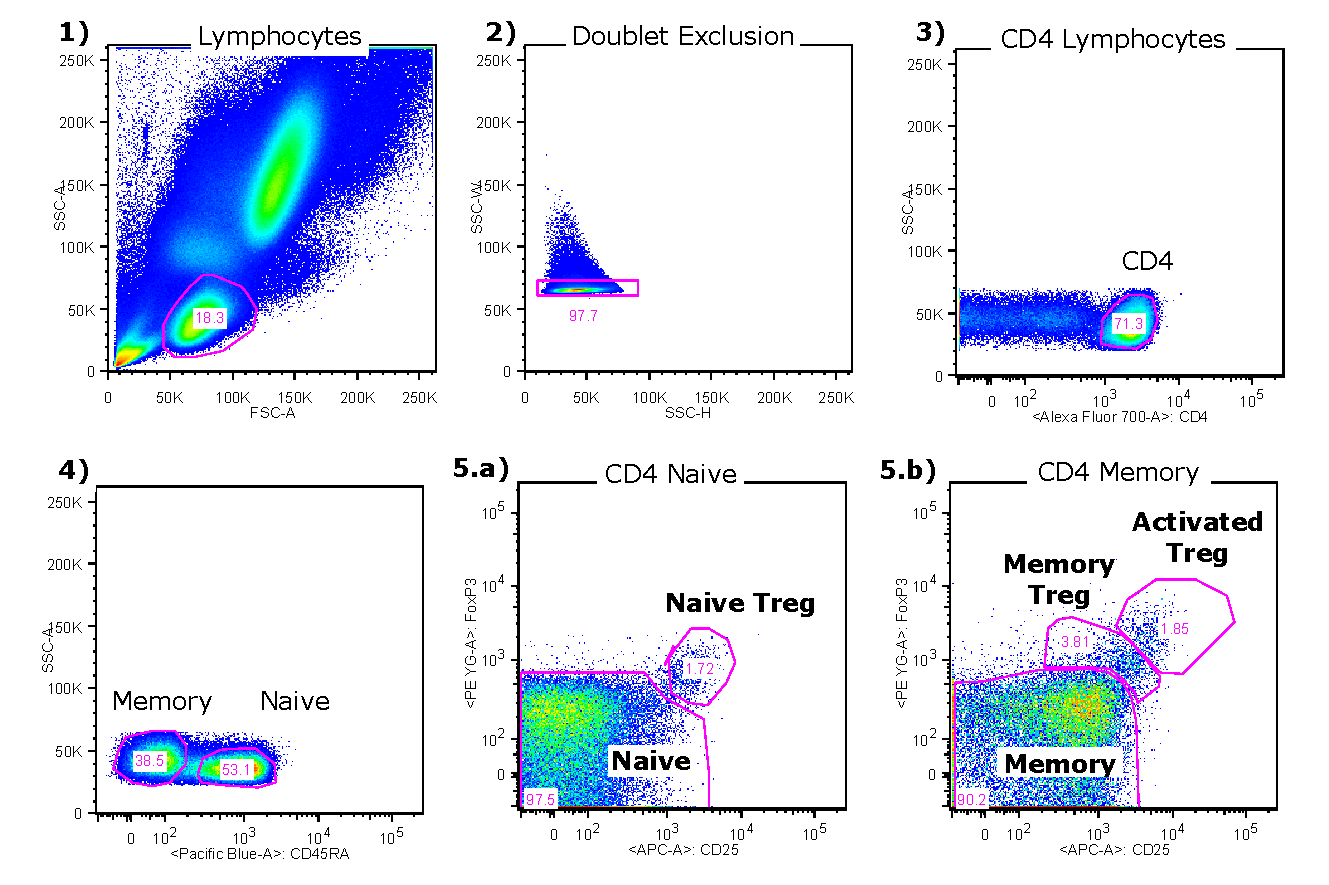
\includegraphics[scale=.75]{IL2/figures/tony-cd4-gating.pdf}
    %\caption{  \label{figure:tony-cd4-gating} Manual gating conducted by \contributor{Tony Cutler} to identify:
    %conventional and regulatory naive and memory T cells as well as activated regulatory T cells.
    %}
%\end{figure}
% 
%\hspace{-2cm}
\begin{figure}[h]
\centering
%\includegraphics[scale=.5]{figures/manual-gating.pdf}
%\begin{subfigure}[b]{.4\textwidth}
%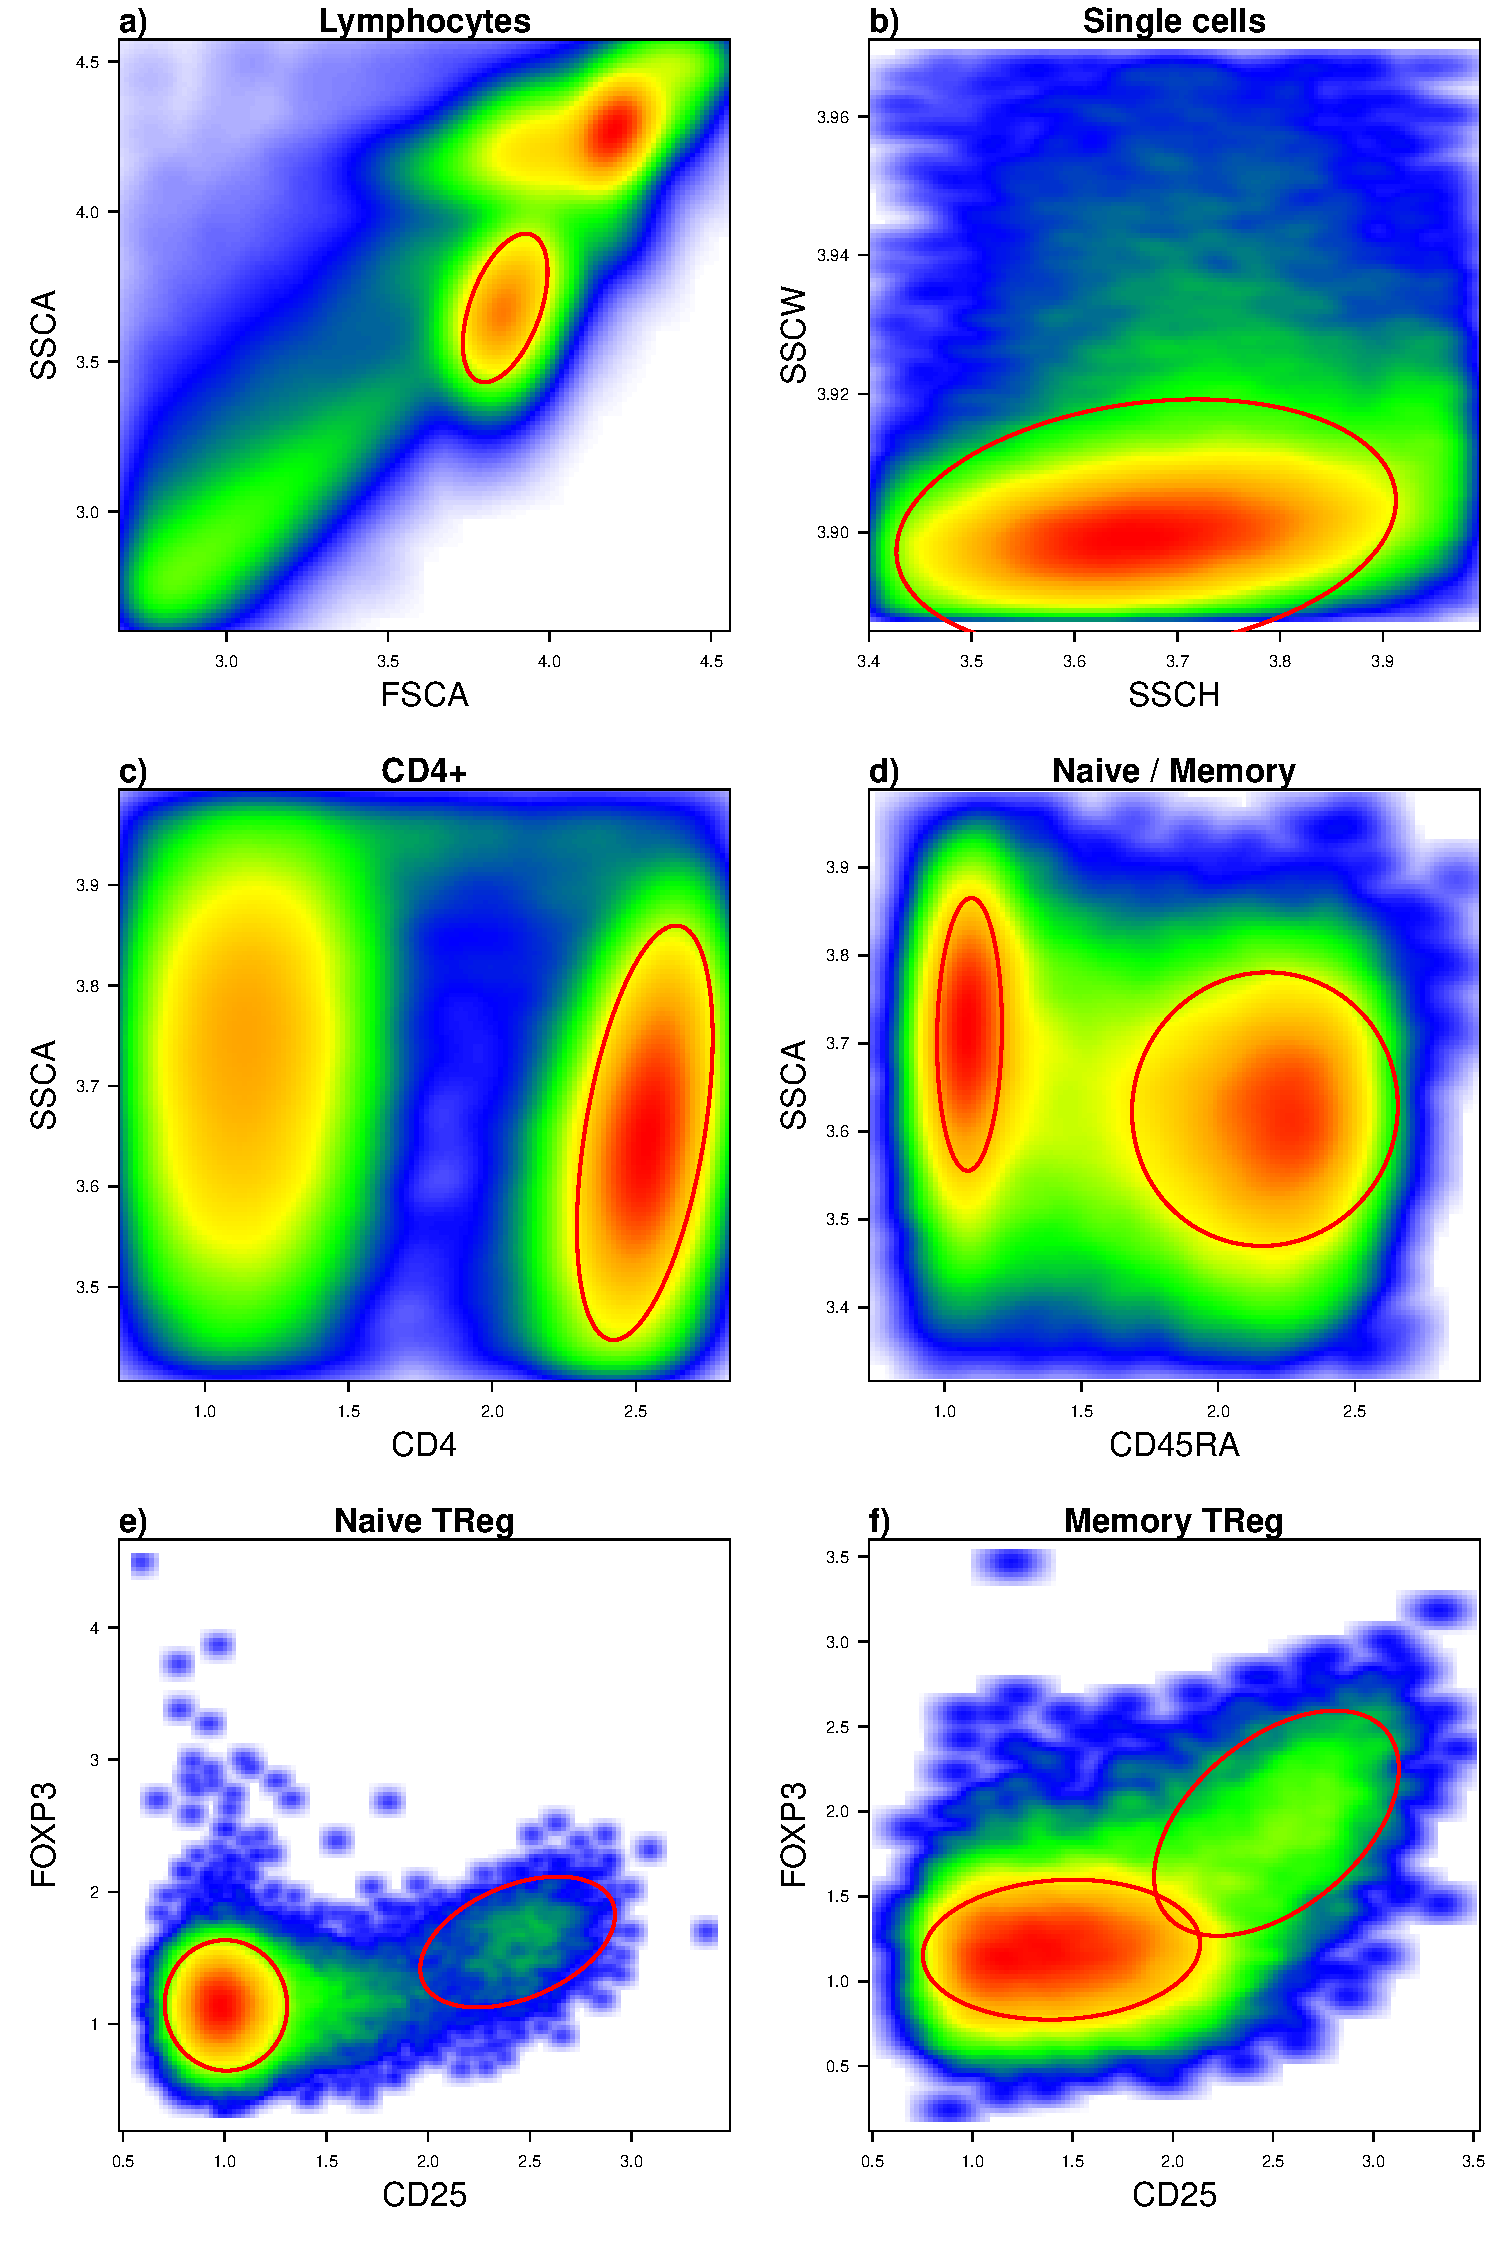
\includegraphics[scale=.25]{IL2/figures/manual-gating-CB00165D_0U_2012-11-29.pdf}
  \includegraphics[scale=.75]{IL2/figures/CB00366X_2012-11-07.pdf}
%\caption{Resting sample.}
%\end{subfigure}
%\begin{subfigure}[b]{.4\textwidth}
%\includegraphics[scale=.25]{IL2/figures/manual-gating-CB00165D_01U_2012-11-29.pdf}
%\caption{Stimulated at 0.1 units of proleukin.}
%\end{subfigure}
%\begin{subfigure}[b]{.4\textwidth}
%\includegraphics[scale=.25]{IL2/figures/manual-gating-CB00165D_10U_2012-11-29.pdf}
%\caption{Stimulated at 10 units of proleukin.}
%\end{subfigure}
%\begin{subfigure}[b]{.4\textwidth}
%\includegraphics[scale=.25]{IL2/figures/manual-gating-CB00165D_1000U_2012-11-29.pdf}
%\caption{Stimulated at 1000 units of proleukin.}
%\end{subfigure}
\mycaption{figure:tony-cd4-gating}
{Gates applied across doses.}
{
Manual gating conducted using FlowJo by \contributor{Tony Cutler} to identify
naive effector (green ellipse) and regulatory T cells (blue ellipse) (e)
and memory effector (black ellipse) and regulatory T cells (red ellipse) (f).
%The same gates can be applied across doses (i, ii, ,iii, iv).
}
\end{figure}
Within each lymphocyte subset, the pSTAT5 distribution was measured, in each of the four samples stimulated at an increasing proleukin dose
(\Cref{figure:dose-effect-pstat5-cellsubsets}).  
As expected, the pSTAT5 distribution shifts progressively right for higher doses of proleukin, as more STAT5 is phosphorylated.
Of the four subsets, the most sensitive cells to proleukin are the smaller memory and naive regulatory T cell subsets (\Cref{figure:dose-effect-pstat5-cellsubsets} b and d),
then the memory effectors (\Cref{figure:dose-effect-pstat5-cellsubsets} a) and finally the naive effectors (\Cref{figure:dose-effect-pstat5-cellsubsets} c).
This correlates with the level of \protein{CD25} expressed by these cells.

%\includegraphics[scale=.45]{IL2/figures/dose-effect-pstat5-cellsubsets-density.pdf}
%\includegraphics[scale=.45]{IL2/figures/dose-effect-pstat5-cellsubsets-density-baseline.pdf}
%\includegraphics[scale=.45]{figures/dose-effect-pstat5-cellsubsets-ecdf-joined.pdf}
\myfigure{scale=.6}
%individual g
{dose-effect-pstat5-cellsubsets-density}
{ Distribution pSTAT5 in the manually gated cell subsets in the sample manually gated in \Cref{figure:tony-cd4-gating}. }
{
The thickness of the lines is representative of the four increasing doses of proleukin (0, 0.1, 10 and 1000 units).
The dose-response is most striking in the smaller Treg subsets with higher CD25 (b and d).
The dashed vertical line represents the 99th percentile of the pSTAT5 distribution in the resting sample,
which is used to define the pSTAT5\positive threshold.
}

Next \contributor{Tony Cutler}, assessed the repeatability of the pSTAT5 response by measuring the pSTAT5 \gls{MFI}
for each individual subset of lymphocytes tested.
However, this cell phenotype was poorly reproducible, since the location of the peaks was not stable across days as illustrated
by the sample shown in \Cref{figure:dose-effect-pstat5-cellsubsets-density-repeatability}.
%Furthermore, the \gls{MFI} is not a representative metric for bimodal distributions 
%However, one issue is that pSTAT5 MFI is not very representative for very bimodal or skewed distributions such
%as the memory effectors in \Cref{figure:dose-effect-pstat5-cellsubsets}.
%Also the resting pSTAT5, which represents the baseline pSTAT5, of the same cell subset may not be constant across days.  
%To address these issues, the percent of pSTAT5\positive cells was also assessed.
\myfigure{scale=.6}
%individual g
{dose-effect-pstat5-cellsubsets-density-repeatability}
{ pSTAT5 distribution in an individual on visit one (black) and visit two (red) clearly shows that pSTAT5 distribution is not stable across days in the four cell
subsets. }
{
In black, the pSTAT distribution on visit one and in red, on visit two.
%The thickness of the line represents the proleukin dose at which the sample was stimulated (0, 0.1, 10 and 1000 units).
The thinner lines are from the resting sample whereas the thicker lines are from the sample stimulated at 1000 units.
The vertical lines represent the pSTAT5\positive threshold set at the $99^{th}$ percentile of the pSTAT5 distribution in the resting sample.
}
This motivated \contributor{Tony Cutler} to instead use a threshold approach to define the ratio of cells which are pSTAT5\positive.
An idea similar to that applied in \Cref{chapter:il2ra} to define naive cells as CD25\positive.
%but the threshold is defined using the unstimulated sample rather than beads. 
%It is a good approach to use when the number of cells is small
%and is commonly used in populations with high CV.
However, here an internal threshold was used, namely
the threshold was defined to be the 99th percentile of the pSTAT5 distribution in the resting cell subset per sample.
Thus each each sample and cell subset had its own pSTAT5\positive threshold.
He presented his results in six of the ten repeated individuals for the four stimulated cell subsets,
memory effector (\Cref{figure:tony-memory-eff}),
memory regulatory T cells (\Cref{figure:tony-memory-treg}),
naive effector (\Cref{figure:tony-naive-eff})
and naive regulatory T cells (\Cref{figure:tony-naive-treg}).
For memory and naive Tregs (\Cref{figure:tony-memory-treg,figure:tony-naive-treg}), at the highest 1000 units dose,
practically all memory and naive tregs are pSTAT5\positive.
However, these cell populations show a significant response already at the lowest 0.1 units dose of proleukin.
Based on this observation, \contributor{Tony Cutler} selected the
memory and naive Treg pSTAT5 cell phenotype to be the percentage of pSTAT5\positive cells at the 0.1 units dose.
On the other hand, since memory effectors are less reponsive, 10 units was chosen as the representative dose.
For naive effectors, the least reponsive of the four cell subsets considered, the repeatability was assessed at the 1000 unit dose.
Tony assessed the repeatability with the coefficient of determination:
%instead of using the square of the Pearson correlation: 
\[
  R^2 = 1 - \frac{\sum_{i=1}^N (x_{i1}-x_{i2})^2}{\sum_{i=1}^N (x_{i1}-\overline{x_1})^2}
\]
where $x_{i1}$ is the phenotype of $i^{th}$ individual on the first day and $x_{i2}$
is the phenotype of the $i^{th}$ individual on the second day.
The coefficient of determination can take negative values if the correlation between $x_{i1}$ and $x_{i2}$ is very low.
Contrary to the Pearson correlation, used in the previous chapter, the coefficient of determination is sensitive to linear transforms.
%this is not correct because it's not symmetric
Even when using the percent of pSTAT5\positive cell phenotype,
the overall reproducibility across the four cell subsets was still poor,
with the more sensitive and smaller cell subsets,
naive and memory Tregs showing the worst correlation ($R^2=-0.16$ and $R^2=-0.82$), memory effectors showing slightly better correlation ($R^2=0.021$)
and finally the less responsive naive effectors showing good correlation ($R^2=0.7728$) (\Cref{figure:tony-repeatability}).
Tony then went on to test association with type 1 diabetes using a two-tailed paired t-test of 20 cases matched with 20 controls analysed on the same
day (\Cref{figure:tony-t1d-association}).
%how did he deal with repeats?
He also tested for association with \gene{IL2RA} SNP \snp{rs12722495}, and the
\gene{PTPN2} SNPs \snp{rs45450798} and \snp{rs478582} (plots not shown).
No significant association was detected either with disease nor with genotype.

\myfigure{scale=.5}
{tony-memory-eff}
{ The percent of pSTAT5\positive cells increases with proleukin dose in memory effectors,
but the measured response is not consistently repeatable (f, g). }
{
  Plot produced by Tony Cutler.
}
\myfigure{scale=.5}
{tony-memory-treg}
{ The percent of pSTAT5\positive cells increases with proleukin dose in memory tregs. }
{
  Plot produced by Tony Cutler.
  While at the highest proleukin dose of 10 and 1000 units, all memory tregs are consistently pSTAT5\positive,
  there is more discrepancy at the low dose of 0.1 units.
}
\myfigure{scale=.5}
{tony-naive-eff}
{ The percent pSTAT5\positive cells increases with proleukin dose in naive effectors. }
{
  Plot produced by Tony Cutler.
  Only \pct{40} of the naive effector cells are pSTAT5\positive even at the highest 1000 unit proleukin dose.
}
\myfigure{scale=.5}
{tony-naive-treg}
{ The percent pSTAT5\positive cells increases with proleukin dose in naive tregs. }
{
  Plot produced by Tony Cutler.
  While at the highest proleukin doses of 10 and 1000 units, all naive tregs are consistently pSTAT5\positive,
  there is more discrepancy at the low dose of 0.1 units.
}
\myfigure{scale=.75}
{tony-repeatability}
{ Repeatability in six individuals }
{
  Plot produced by Tony Cutler.
  The repeatability of the percent of cells which are pSTAT5\positive is assessed in effector memory and naive at the 10U and 1000U dose
  respectively, and in memory and naive regulatory T cells at the 0.1U dose.
  While the repeatability in the naive effector subset was good ($R^2=0.7728$), the repeatability in the other cell subsets is poor
  (memory effectors $R^2=0.021$, naive tregs $R^2=-0.16$ and memory tregs $R^2=-0.82$).

}
\myfigure{scale=.75}
{tony-t1d-association}
{ Association test of percent pSTAT5\positive in four cell subsets. }
{
  Plot produced by Tony Cutler.
  The association with T1D of the percent of cells which are pSTAT5\positive is assessed in effector memory and naive at the 10U and 1000U dose
  respectively, and in memory and naive regulatory T cells at the 0.1U dose.
  The association test is a two-tailed paired-t-test on 20 cases paired with 20 controls analysed on the same day (40 out of the available 96 individuals).
  No significant association is detected.
}

%\section{Automatic methods}
%\subsection{Normalisation of pSTAT5 improves repeatability}
\section{Reproducibility of pSTAT5 response within an individual}

Tony's preliminary results in the six repeated individuals suggested that the pSTAT5 MFI and percent pSTAT5\positive were poorly reproducible
cell phenotypes using the methodology and approach described, which consequently would give us little power to detect an association with disease status or genetics.
This motivated me to see if I could improve the repeatability of these cell phenotypes using normalisation.
%Furthermore, since these cell phenotypes were only defined at a single dose, I also defined new cell phenotypes to summarise the response across doses.
I evaluated the reproducibility of these cell phenotypes with different normalisation approaches.

\subsection{Normalisation approaches}

%I attempted to use normalisation to improve the repeatability of the proleukin response measure.
Here I describe the methods I considered.

\paragraph{Bead normalisation} 
In \Cref{chapter:il2ra}, I used beads to correct for day to day variation in the CD25 channel.
However for the stimulation data, beads in the Alexa-488 channel, the fluorochrome conjugated to pSTAT5 (\Cref{table:IL2-panels}),
%\Cref{chapter:il2ra}
did not adequately capture the short term variation in pSTAT5 (\Cref{figure:pstat5-beads}).  
%This suggests that for this experiment, flurorescent beads do not explain the day to day variation in the pSTAT5 MFI.
\begin{figure}[h]
    \centering
    %\includegraphics[scale=.5]{IL2/figures/beads.pdf}
    %\includegraphics[scale=.5]{IL2/figures/beads.pdf}
    %\includegraphics[scale=.75]{figures/alexa488-beads.pdf}
    \includegraphics[scale=.6]{figures/pstat5-beads.pdf}
    \mycaption{figure:pstat5-beads}
    {Variation in sample MFI is not captured by variation in bead MFI.}
    {
      For the purpose of MFI normalisation, the fluorescence intensity of six-peak flow cytometry beads
      was measured in the Alexa 488 channel, the fluorochrome conjugated to the pSTAT5 marker.
      However, as illustrated by the loess lines, the beads are not appropriate for pSTAT5 normalisation,
      since the MFI of the three dimmest populations of beads (orange)
      does not capture the pSTAT5 MFI time variation in the four cell subsets.
      The pSTAT5 MFIs are obtained from samples stimulated at 1000 units of proleukin.
      
    }
\end{figure} 


\paragraph{ Correcting for baseline MFI }
One observation which can be drawn from \Cref{figure:dose-effect-pstat5-cellsubsets-density-repeatability} is that the
MFI of the pSTAT5 distribution in the resting sample is different across days.
If a cell population had a higher resting pSTAT5 MFI due only to day to day variability,
then one might expect that the pSTAT5 MFI in the stimulated population would also be higher.
%First I noticed that Tony had not corrected for baseline MFI.
I first attempted to account for the difference in resting pSTAT5 by subtracting the MFI of the resting population from the MFI of
the stimulated populations.
Since fluorescence intensity scales multiplicately, I also attempted to do the correction by dividing by the baseline MFI
or alternatively by subtracting the log transformed MFIs.
However, this did not appear to improve the repeatability significantly but instead just reduced the MFI by the same factor on both days
(\Cref{figure:pstat5-mfi-cellsubsets-repeatability}).
This suggests that the day to day variation in the resting sample MFI does not capture the variation in the stimulated population
.
\myfigure{scale=.75}{pstat5-mfi-cellsubsets-repeatability}
{ pSTAT5 MFI (black), background subtracted pSTAT5 MFI (red) }
{
  Correcting for the MFI in the resting sample does not appear to improve the repeatability significantly but instead just reducing the MFI by
  the same factor on both days.
  This suggests that the day to day variation in the resting sample MFI does not explain the variation in the stimulated population.
}

\clearpage

\paragraph{Nearest-neighbour joining}
%While using a different background MFI should account for differences in resting MFI,
%this assumes that the MFI difference is representative of the pSTAT5 shift.
%This may not be true for distributions which change modality.
One concern is that the difference in population cell counts across samples stimulated at different doses, may influence the accuracy of the MFI estimate.
Another concern is that since the pSTAT5 distribution is often bimodal in the cell populations considered, substracting the MFI may not be ideal.
Instead, a more correct approach would be to subtract the pSTAT5 fluorescence intensity for each resting cell.
One way of emulating this is to match each cell to its closest neighbour in the unstimulated sample.  
This was accomplished by joining samples on their core markers using the \gls{ANN} to the resting sample \citep{Jones:2011ez}
as implemented in the \Rpackage{RANN}.
This created a dataset of the same number of cells as the resting dataset, but where each cell now had a total of four functional pSTAT5 markers,
one for each stimulation dose.
At each cell it is now possible to assess the difference in pSTAT5 response between resting and stimulated states.
This is important because cells do not all have the same resting level of pSTAT5 (\Cref{figure:pstat5-baseline-relative}).
This approach presents a number of advantages.
Firstly, only the sample to which the other samples are joined needs to be gated.
Secondly, since the pSTAT5 response is relative to the baseline, it should be more robust to variation between days
and consequently, more reproducible than pSTAT5 fluorescence intensity.
Thirdly, since we have response at the cell-level, we can use methods
such as \gls{CART}, \gls{RF} and \gls{MARS} to do multivariate regression of pSTAT5 from core markers.
This could help identify cells which would have been missed from only examining core markers.
%However, even when we correct for the different baseline, the distance between the peak of the resting sample and the stimulated sample is not constant
%figure
%An advantage of this method is that number of cells per cell type is constant across doses.
%A disadvantage of this method is that the number of cells is very different of that all the cells are shifted then they will all be joined to closest neighbour
%which could be a single point.
%which will investigate in the second section.
%An alternative to this approach, would be to gate subsets in subsamples stimulated at different doses and subtract the background,
%however a clear advantage of this approach is that it allows for methods such as RF and MARS
The \gls{ANN} approach is valid without normalisation since the distributions of the core markers align across doses.
%(\Cref{figure:core-markers}).
%\Cref{figure:ann-join-0U-01U} confirms that the mapping of the clusters is correct across the nearest-neighbour mapping.
%When the between-dose variation on the core markers is negligeable,
%If we assume that the within-tube variation is negligeable, then a simpler solution is possible:
%each cell in the unstimulated subsample is joined to its closest neighbouring cell (in terms of its core markers) in a stimulated subsample.
%This assumes that the core markers are fairly stable across samples, which is usually the case in ex-vivo stimulated.
%The joining results is also not affected by any euclidean distance preserving transform, so the FCS data can be transformed before or after the \gls{ANN} joining.
%Another important check is to see whether the joining is sensitive to the transform.
%We find that we get the same results whether we join before or after the transform.
%\myfigure{scale=.3}{dose-effect-core-markers}{Dose-effect on core markers in ungated sample.} { Increasing doses represented by lines of increasing thickness.  The distributions align well across doses.  }
However, using this nearest-neighbour joining method, the repeatability of the cell phenotypes pSTAT5 MFI (\Cref{figure:nn-pstat5-mfi-cellsubsets-repeatability})
and the percent of pSTAT5\positive (\Cref{figure:pstat5-pos-cellsubsets-repeatability}) are not substantially improved.


%
%\myfigure{scale=.3}{ann-join-0U-01U}
%{ Nearest neighbour join on core markers of ungated resting sample with ungated sample stimulated at 0.1 units. }
%{
%All clusters lie on the y=x line which suggests that the largest clusters are correctly matched across samples.
%}
%
\myfigure{scale=.5}{pstat5-baseline-relative}
{ pSTAT5 intensity across the four proleukin doses, before (a) and after (b) per-cell baseline pSTAT5 subtraction in the ungated sample.}
{
  An important proportion of cells are already saturated for pSTAT5 (high baseline) in the resting sample (a).
  Correcting for the per cell pSTAT5 baseline, shows the true proportion of cells which responds to proleukin within this sample (b).
}
%
\myfigure{scale=.75}{nn-pstat5-mfi-cellsubsets-repeatability}
{ Repeatability of pSTAT5 MFI in the nearest-neighbour joined (black), nearest-neighbour background subtracted (red). }
{
  %nearest-neighbour joined samples (black)
  %nearest-neighbour joined samples baseline corrected (red)
  Background subtraction does no substantially improve the repeatability of the pSTAT5 MFI phenotype.
}
%
\myfigure{scale=.75}{pstat5-pos-cellsubsets-repeatability}
{ Repeatability of percent pSTAT5\positive in the individual samples (black), nearest-neighbour joined (red) and nearest-neighbour joined samples baseline corrected (blue). }
{
}
%\myfigure{scale=.75}{pstat5-mfi-auc-celltypes}
%{ pSTAT5 MFI for each normalisation method.  }
%{
  %The solid lines represent the median.
  %The shaded areas represent the 25th and 75th percentile.
  %The doses at which most of the variation occurs are 1000 units for naive effectors (green),
  %10 units for memory effectors (black), 0.1 units for memory (red) and naive (blue) regulatory T cells.
  %%a) The dose-response curve for each cell type in all samples.
  %%b) The medians dose-response curve across all samples for each cell type.
%}
%\myfigure{scale=.7}{pstat5-pos-auc-celltypes}
%{ Percent pSTAT5\positive for each normalisation method. }
%{
  %The solid lines represent the median.
  %The shaded areas represent the 25th and 75th percentile.
  %The doses at which most of the variation occurs are 1000 units for naive effectors (green),
  %10 units for memory effectors (black), 0.1 units for memory and naive regulatory T cells.
  %%a) The dose-response curve for each cell type in all samples.
  %%b) The medians dose-response curve across all samples for each cell type.
  %%There are many samples which stand out as outliers and a few of them have been misgated.
%}
%
%\myfigure{scale=.5}{pstat5-auc-boxplots-celltypes.pdf} { Influence of normalisation method on pSTAT5 area under curve. } { In red the normalisation using the peak alignment in CD4\positive lymphocytes, in blue the normalisation using peak alignment in lymphocytes. }
%\begin{figure}[h]
    %\centering
    %\includegraphics[scale=.5]{IL2/figures/pstat5-auc-repeatability-celltypes.pdf}
    %\mycaption{figure:pstat5-auc-repeatability-celltypes}
    %{ Influence of normalisation on the repeatability of the pSTAT5 area under the curve. }
    %{ In red the normalisation using the peak alignment in CD4\positive lymphocytes, in blue the normalisation using peak alignment in lymphocytes. }
%\end{figure}
\clearpage



\subsection{Repeatability}


For all ten repeated samples, the Pearson correlation squared $r^2$ of the MFI was assessed at the four increasing doses, in the four cell subsets,
for the raw (\Cref{figure:repeatability-PSTAT5-MFI}a),
baseline corrected (\Cref{figure:repeatability-PSTAT5-MFI}b),
nearest-neighbour joined (\Cref{figure:repeatability-PSTAT5-MFI}c)
and nearest-neighbour baseline corrected (\Cref{figure:repeatability-PSTAT5-MFI}d).
The repeatability of the percent pSTAT5\positive across doses gives a different pattern depending on the cell type
but at the highest dose it appears that the least responsive naive effector cells yield the best
repeatability (\Cref{figure:repeatability-PSTAT5-pos}).
Suprisingly, the memory regulatory T cells have the highest repeatability at the 0.1 unit dose.
The repeatability of the naive regulatory T cell phenotype is poor at all doses.  
The NN joining does not significantly improve the repeatability (\Cref{figure:nn-pstat5-mfi-cellsubsets-repeatability}).
No normalisation approach stands out as improving the repeatability.

\myfigure{scale=.5}
{repeatability-PSTAT5-MFI}
{
  Repeatability of pSTAT5 MFI measured as Pearson correlation squared ($r^2$) per dose per cell type.
}
{
  On subtracting the baseline, the repeatability of the naive effector subset is improved but not in the other cell subsets.
} 
\myfigure{scale=.5}
{repeatability-PSTAT5-pos}
{
  Repeatability of the percent of pSTAT5\positive as Pearson correlation squared ($r^2$) per dose per cell type.
}
{
  Only the pSTAT5 in the naive effector subset stimulated at 100U shows good repeatability across all normalisation methods.
  %While the repeatability of the percent pSTAT5\positive is more reproducible.
}

%
%\hspace{-2cm}
%\begin{figure}[h]
%\centering
%\includegraphics[scale=.4]{IL2/figures/pstat5-response-cellsubsets-manualgates.pdf}
%\caption{ \label{figure:pstat5-response-cellsubsets-gate}
%Fixed gates (a and b), magnetic gates (c and d).
%The response is measured in terms of baseline relative pSTAT5 MFI.
%a) The dose-response per cell-type in each sample obtained from manual gating with fixed gates.
%Note the outstanding memory effector sample is due to poor gating of the memory populatin in that particular sample.
%%CB01500E
%This in part due to the gate position but also because that sample does not have a clear memory population.
%b) The median dose-response per cell-type obtained from manual gating with fixed gates.
%}
%\end{figure}
%

%\section{pSTAT5 response metrics}
%\section{pSTAT5 response in the manually gated cell subsets} 
%\section{Joining samples on core markers using approximate nearest-neighbour}

%\hspace{-2cm}
%\begin{figure}[h]
%\centering
%%\includegraphics[scale=.5]{figures/manual-gating.pdf}
%\begin{subfigure}[b]{.4\textwidth}
  %\includegraphics[scale=.25]{IL2/figures/repeatability-pstat5-mfi-Memory-Eff.pdf}
%\caption{Memory Effector}
%\end{subfigure}
%\begin{subfigure}[b]{.4\textwidth}
  %\includegraphics[scale=.25]{IL2/figures/repeatability-pstat5-mfi-Memory-Treg.pdf}
%\caption{Memory Treg}
%\end{subfigure}
%\begin{subfigure}[b]{.4\textwidth}
  %\includegraphics[scale=.25]{IL2/figures/repeatability-pstat5-mfi-Naive-Eff.pdf}
%\caption{Naive Effector}
%\end{subfigure}
%\begin{subfigure}[b]{.4\textwidth}
  %\includegraphics[scale=.25]{IL2/figures/repeatability-pstat5-mfi-Naive-Treg.pdf}
%\caption{Naive Treg}
%\end{subfigure}
%\caption{
%\label{figure:repeatability-gating}
%In black manual gates, in red magnetic gates.
%The AUC is the area under the dose response curve.
%}
%\end{figure}
%

%In the manual analysis conducted by Tony Cutler, he found that he could identify individuals which were low or high responders.
%This leads us to hypothesise that within one individual the response to \emph{IL-2} on day 1 should be comparable to the response to \emph{IL-2} on day 2.

%One method we have tried is based on the assumption is that in the ungated data, the bottom and top percentile of the pSTAT5 distribution do not respond to \emph{IL-2} and so can be used as reference points.  This is effectively a quantile normalisation method aligning the bottom and top percentile across doses.

%However we found that this normalisation method d is not true in CD4+ lymphocyte gated data.  
%Certain normalisation methods make assumptions about the shape of the data.
%The actual choice of normalisation depends on the characteristics of the data we wish to compare.
%Certain normalisation methods such as quantile normalisation are not appropriate since they assume the distributions have the shame shape.


%\begin{figure}[h]
%%
%%#simulated data
%%x0 <- mixtools::rnormmix(1000, mu=c(1,6), lambda=c(.3,.7))
%%x1 <- mixtools::rnormmix(1000, mu=.9*c(1,6)+2, lambda=c(.5,.5), sigma=c(2,2))
%%d0 <- density(x0)
%%d1 <- density(x1)
%%l0 <- extract.landmarks(x0,max.lms=2, bw=d0$bw)
%%l1 <- extract.landmarks(x1,max.lms=2, bw=d1$bw)
%%m <- lm(l0$lms ~ l1$lms)
%%x1.norm <- cbind(1,x1)%*%coefficients(m)
%%l1.norm <- extract.landmarks(x1.norm,max.lms=2)
%%#before align
%%pdf('~nikolas/GoogleDrive/PhD/Thesis/IL2/figures/simulation-peak-align-noise.pdf')
%%plot(d0,xlim=c(-3,11),main='', xlab='')
%%points(l0$lms, l0$dens, pch=20, cex=2)
%%lines(d1, lty=2)
%%points(l1$lms, l1$dens, pch=20, cex=2)
%%#after peak align
%%lines(density(x1.norm), lty=2, col='red')
%%points(l1.norm$lms, l1.norm$dens, pch=20, cex=2, col='red')
%%dev.off()
%%
    %\centering
    %\includegraphics[scale=1]{IL2/figures/simulation-peak-align-noise.pdf}
    %\caption{  \label{figure:simulation-peak-align-noise}  In solid black line represents the density function obtained from $1000$ draws from a mixture of two normal distribution
    %with means $\mu_0=(1,6)$, standard deviations $\sigma_0=(1,1)$ and mixing proportions $\tau_0=(.3,.7)$.
    %The dashed black line represents the density function obtained from $1000$ draws from a mixture of two normal distribution
    %where $\mu_1 = 0.9 \mu_0 + 2$, standard deviations $\sigma_0=(1,1)$ and $\tau_1=(.5,.5)$.
    %The red dashed line represents the transformation using peak alignment. }
%\end{figure}
%

%%e <- lapply(flat.rep.fcs[names(flat.rep.fcs)[1:4]], function(x) ecdf(lgcl(getChannels(x, 'pstat5'))))
%%d <- lapply(flat.rep.fcs[names(flat.rep.fcs)[1:4]], function(x) density(lgcl(getChannels(x, 'pstat5')),bw=.1))
%%d.f <- lapply(d, function(d) splinefun(d$x,d$y))
%%y.max <- max(sapply(d, function(d) d$y)) 
%%e <- lapply(lymph[names(lymph)[1:4]], function(x) ecdf(lgcl(getChannels(x, 'pstat5'))))
%%d <- lapply(lymph[names(lymph)[1:4]], function(x) density(lgcl(getChannels(x, 'pstat5')),bw=.1))
%%d.f <- lapply(d, function(d) splinefun(d$x,d$y))
%%y.max <- max(sapply(d, function(d) d$y)) 
%%#pdf('~nikolas/lymph-dose-effect.pdf',width=10,height=5)
%%pdf('~nikolas/ungated-dose-effect.pdf',width=10,height=5)
%%par(mfrow=c(1,2))
%%x <- seq(-.5, 3, length.out=20000)
%%plot(x, e[[1]](x), col='white', xlab='pSTAT5', xlim=c(-.5,3), ylab='') 
%%mapply(function(e,lwd,lty) lines(x,e(x),lwd=lwd,lty=lty),e,seq(1,2.5,.5),c(1,2,2,1))
%%legend('topleft',doses, lwd=seq(1,2.5,.5), lty=c(1,2,2,1))
%%plot(x, d.f[[1]](x), col='white', xlab='pSTAT5', xlim=c(-.5,3),ylim=c(0,1),ylab='') 
%%mapply(function(d,lwd,lty) lines(x,d(x),lwd=lwd,lty=lty),d.f,seq(1,2.5,.5),c(1,2,2,1))
%%legend('topleft',doses, lwd=seq(1,2.5,.5), lty=c(1,2,2,1))
%%dev.off() 
%%pdf('~nikolas/ungated-lymph-dose-effect.pdf')
%%par(mfrow=c(1,1))
%%x <- seq(-.5, 3, length.out=20000)
%%plot(x, d.f[[1]](x), col='white', xlab='pSTAT5', xlim=c(-.5,3),ylim=c(0,1),ylab='') 
%%d <- lapply(flat.rep.fcs[names(flat.rep.fcs)[c(1,4)]], function(x) density(lgcl(getChannels(x, 'pstat5')),bw=.1))
%%d.f <- lapply(d, function(d) splinefun(d$x,d$y))
%%y.max <- max(sapply(d, function(d) d$y))
%%mapply(function(d,lwd,lty) lines(x,d(x),lwd=lwd,lty=lty),d.f,c(1,2.5),1)
%%d <- lapply(lymph[names(lymph)[c(1,4)]], function(x) density(lgcl(getChannels(x, 'pstat5')),bw=.1))
%%d.f <- lapply(d, function(d) splinefun(d$x,d$y))
%%y.max <- max(sapply(d, function(d) d$y))
%%#r <- mapply(function(a,b) length(a)/length(b), lymph[1:4], flat.rep.fcs[1:4])
%%mapply(function(d,lwd,lty) lines(x,d(x),lwd=lwd,lty=lty,col='red'),d.f,c(1,2.5),1) 
%%legend('topleft',doses[c(1,4)], lwd=c(1,2.5), lty=1)
%%dev.off()
%%lymph <- sapply(flat.rep.fcs, function(x) { cd4 <- lgcl(getChannels(x, 'cd4')); return(x[2 <  cd4 & cd4 < 2.75,]) })
%%

\subsection{Association of pSTAT5 response with type 1 diabetes}

I tested the association with T1D at each dose as well as for the area under the curve.
%Having improved the reproducibility of the cell phenotype with normalisation via peak alignment,
%we are now in a position to test the original hypothesis of whether type 1 diabetics show a reduced response to proleukin in those cell subsets.
I accounted for repeated individuals and day of analysis by including them as random effects in a linear mixed effects model as applied in \Cref{chapter:il2ra}.
%\Cref{chapter:il2ra}.
%\contributor{Hui Guo} also attempted a stratified boostrapping to compute the variance for a paired-test
%Using the paired design, we also control for sex and day of analysis.  
%Having not identified a significant association, this now brings us to the next question of whether there are other
%cell subsets besides the ones which we are gating which are sensitive to proleukin, and in particular low doses of proleukin?
%Unsuprisingly, given the small sample size and the poor reproducibility of the assay,
No T1D association was detected with the pSTAT5 MFI 
(\Cref{figure:pstat5-mfi-t1d-celltypes,figure:nn-pstat5-mfi-t1d-celltypes})
nor with the percent pSTAT5\positive
(\Cref{figure:pstat5-pos-t1d-celltypes,figure:nn-pstat5-pos-t1d-celltypes})
cell phenotypes in the four cell subsets considered.

%\begin{figure}[h]
    %\centering
    %\includegraphics[scale=.5]{IL2/figures/pstat5-auc-t1d-celltypes.pdf}
    %\mycaption{figure:pstat5-auc-t1d-celltypes}
    %{ Influence of normalisation on the association of pSTAT5 area under the curve with type 1 diabetes in the four cell subsets. }
    %{ }
%\end{figure} 

% pSTAT5 MFI
%\hspace{-2cm}
\myfigure{scale=.7}{pstat5-mfi-t1d-celltypes}
{ Association test of pSTAT5 MFI with T1D. }
{ }
\myfigure{scale=.7}{nn-pstat5-mfi-t1d-celltypes}
{ Association test of pSTAT5 MFI, after nearest-neighbour normalisation, with T1D. }
{ }
{ }

% pct pSTAT5+
\myfigure{scale=.7}{pstat5-pos-t1d-celltypes}
{ Association test of percent pSTAT5\positive with T1D. }
{ }
\myfigure{scale=.7}{nn-pstat5-pos-t1d-celltypes}
{ Association test of percent pSTAT5\positive, after nearest-neighbour normalisation, with T1D. }
{ } 


\section{Response in the whole sample}

%\begin{figure}[h]
    %\centering
    %\includegraphics[scale=.5]{IL2/figures/ungated-dose-effect.pdf}
    %\includegraphics[scale=.5]{IL2/figures/lymph-dose-effect.pdf}
    %\mycaption{figure:dose-effect}
    %{Dose effect.}
    %{
        %On the left the cumulative density function obtained from individual a on day 1 across 4 increasing doses.
        %On the right the density function.
        %The top two figures are from the ungated sample.
        %The bottom two figures are from a CD4 range gate.
        %We observe that in the unstimulated sample the distribution is already bimodal 
        %and that upon stimulation the location of the peaks does not change much but that the height changes greatly.
        %Contrary to the ungated data, the pSTAT5 distribution in the CD4 gated sample now appears unimodal when resting or stimulated
        %at the lowest 1U dose.  At the higher doses we start seeing a bimodal distribution.
        %In the ungated sample, the location of the activation peak seems to align somewhat with that of the activation peak.  }
%\end{figure}
%
%In \Cref{figure:dose-effect} we observe that at the lowest 0.1U dose there seems to be a much more stronger relative repsonse
%in the whole sample than in the lymphocyte subset which suggests that there exist other cells beside CD4\positive lymphocytes
%which are also responsive to low doses of IL-2.  
%However the relative difference in response between 10U and 1000U seems much more important in lymphocytes than in the whole sample
%suggesting that the non-CD4\positive lymphocytes in the whole sample reach saturation at 0.1U.
%Also since the resting sample sample displays a shoulder this suggests a mixture of resting and already semi-activated lymphocytes.
Using the methods described in the previous section, I failed to significantly improve the reproducibility of this assay.
This implies that this dataset is unlikely to be useful for association testing.
However, it still contains useful biological information.

DILT1D and other clinical trials of IL-2 have largely focused on lymphoyctes. %CD4\positive cells.
However, biologists know that any cell which carries high levels of any of the trimeric components of the IL-2 receptor,
alpha (CD25), beta (CD122) or gamma (CD132), should respond to IL-2, however
due to limitations on the binding affinity of the CD122 antibody and the number of fluorochromes per tube,
they cannot all be included as part of every flow experiment.  
%Plus at low doses of IL-2 the CD25 chain is the most important
%Also the gamma chain is expressed by all cells and so not specific
This study of \emph{ex vivo} stimulated whole blood offers a chance to explore potentially new cell subsets responsive to IL-2.
To increase my chances of characterising unstudied cells subsets, I analysed the subset of samples stained with the more comprehensive marker panel containing
the additional fluorochromes CD3, CD8 and CD56 (\Cref{table:IL2-panels}).
%which is only available in a subset of samples.
%Given the markers used in this study, I was interested in finding out if I could identify other cell subsets which are sensitive to proleukin.
%We are interested in identifying and classifying cell subsets by their sensitivity to proleukin.  
When assessing the dose-response to stimulation in a flow cytometry sample,
the classic approach is to gate cell populations in each sample based on their core markers,
and then assess the response of the functional marker in the gated subset.
However, this approach may miss other dose-responsive cell populations which are not included in the gating.
%This might be solved by exhaustive gating
Here I will first explore approaches to visualise the pSTAT5 dose-response in the whole sample,
then I will consider automated gating methods which use the pSTAT5 response to guide the identification of cell subsets.
%While the manual gating inspired approach is the established method, it suffers from a major drawback:
%it relies on prior knowledge of the number of cell populations and consequently misses the pSTAT5 response in uncharacterised cell subsets.


\subsection{Visualising response in whole sample with \acrfull{SPADE}}

Researchers working in low dimensional data typically begin with visualisation.
This is also important in high dimensional data but needs more innovative approaches.
I wanted to visualise the dose-response in the whole sample.
%\Gls{MDS} methods can give us an two-dimensional representation of a higher dimensional data set from a distance matrix.
Dimensionality reduction methods can provide a two-dimensional representation of a higher dimensional data set from a distance matrix.
%There are well established linear ones such as \gls{PCA} but also nonlinear ones such as \gls{ISOMAP} \citep{Tenenbaum:2000jp}.
These methods are particularly popular for datasets with less data points but more dimensions than flow cytometry,
as generated by mass cytometry technologies such as CytoF.
In mass cytometry datasets, more emphasis is given on uncovering cell lineages and progressions rather than discrete cell populations which share marker
properties.
Most of these methods, like \gls{MDS}, require computation of the complete pairwise distance matrix,
but some like \gls{PCA} can use the covariance matrix instead to identify the components which accounts for most of the variation. 
%Stochastic neighbour embedding attempts to preserve the proximity of objects in higher dimensional space by using probabilistic mapping of higher dimension space to lower dimension.
%A drawback is that the mapping is impossible to retrieve, which is why component methods like PCA and ICA are more interpretable.  
However, information is lost when considering only the first two components of a linear projection.
Therefore, there is considerable interest in developing methods that capture both the local and global structure of the data,
so that points which lie close in higher-dimensional space tend to lie close in two-dimensional space.
%\gls{ISOMAP} \citep{Tenenbaum:2000jp}.
%SPADE is a methods which was developed with this objective.
In flow cytometry, one such method is \acrfull{SPADE} which gives a \acrfull{MST} representation,
where each node in the tree represent a multi-dimensional cluster in flow marker space \citep{Simonds:2011jh}.
The \gls{MST} is defined as the shortest path that connects all points in a network.
%The visualisation requires requires downsampling.
%A soft approach to downsampling, is to downweight points in high-density regions
The computation of the \gls{MST} necessitates the complete distance matrix which is not feasible for most ungated flow cytometry samples.
%since the number of data points far exceeds.
Hence \gls{SPADE} first needs to reduce the number of data points by making use of downsampling and clustering.
In order for all existing regions of the marker space to be equally represented in the reduced dataset,
the density is normalised across the sample.
At each data point, the multivariate density is estimated, then the number of points is reduced by preferentially removing 
points with high local density while preserving lower density ones.
%Hence the density is more uniform across the sample.
%This is that the density has less influence on the clustering.
Once the number of points has been reduced to some target number or by some factor, in each individual sample,
the samples are pooled and agglomerative clustering is applied.
%further reducing the number of data points to set number .
%The overall number of clusters can then be selected by cutting the resulting dendogram at the required height.
%The default parameter is 300 clusters.
The distance matrix is then calculated on the clusters and they are joined as nodes by the \acrfull{MST} algorithm for the purpose of visualisation.
%Once the MST has been constructed,
The points from each sample which were discarded in the density normalisation step, are then added back and assigned to their closest node in the tree.
%Hence the size of each cluster is sample dependent.
Hence the structure of the tree is the same across all samples but the size of the tree nodes 
is dependent on the number of data points assigned to each node per sample.
The tree nodes can then be coloured according to the intensity of a functional marker, for example here pSTAT5,
which was not used in its construction.
Two steps of the algorithm require user specified parameters, the parameter that defines the downsampling,
which can either be a target number of data points of a factor, and parameter that defines the number of desired clusters
in the agglomerative clustering step.

\subsubsection{Lymphocytes}

I first ran \gls{SPADE} on the manually gated lymphocyte subset (excluding doublets),
in the resting and stimulated stimulated samples from an individual.
The algorithm was run on the core surface markers, CD25, CD3, CD4, CD45RA, CD56, CD8 and FOXP3,
which are expected to be stable across within-batch stimulation doses.
The number of events in each sample was reduced by a factor of 90 percent.
The desired number of cluster in the agglomerative step was set to 1000.
The resulting \gls{MST} was layed out and displayed using the \Rfunction{SPADE.layout.arch}
which aims to orientate the longest branch of an \gls{MST} along an arch with shorter offshoot branches hanging below.
The nodes in the tree were then coloured according to the fold increase in median pSTAT5 compared to the same node
in the resting sample (\Cref{figure:spade-lymphocytes-pstat5mfi}).
%The color scale was chosen to go from dark blue to red and the range was divided in percentiles.
%The output is presented in \Cref{figure:spade-lymphocytes-pstat5mfi}.
%In the unstimulated sample, th(\Cref{figure:spade-lymphocytes-pstat5mfi}a)
The initial pSTAT5 response to the lowest $0.1$ units dose proleukin, clusters in two regions of the tree,
as seen in \Cref{figure:spade-lymphocytes-pstat5mfi}b.
As the stimulation dose is increased to $10$ units, the level of the response increases in these two regions,
and there are signs of response in further adjacent nodes of the tree (\Cref{figure:spade-lymphocytes-pstat5mfi}c).
Finally at the highest dose of $1000$ units, the majority of the nodes show some level of response (\Cref{figure:spade-lymphocytes-pstat5mfi}d).

\myfigure{scale=.7}{spade-lymphocytes-pstat5mfi}
{\gls{MST} generated by applying \gls{SPADE} on lymphocytes. The nodes of the \gls{MST} are coloured by pSTAT5 \gls{MFI}.}
{
  The \gls{MST} was constructed from running \gls{SPADE} on the core surface markers,
  CD25, CD3, CD4, CD45RA, CD56, CD8 and FOXP3, in the manually gated lymphocyte subset (after double exclusion),
  pooled across the four stimulation doses in a sample from one individual.
  The required number of clusters in the agglomerative clustering step was set to k=1000.
  %The size of each node in the tree is representative of the number of cells which are assigned to that cluster. 
  The colouring of the nodes from dark blue to bright red follows the pSTAT5 MFI fold increase.
  In samples where the proleukin dose is increased, more nodes in the tree are illuminated since the pSTAT5 MFI increases in various cell subsets.
  The size of the tree nodes are proportional to the number of cells in the data file which are assigned to that node.
}

In order to discover where the responsive cells lie on the tree in relation to the cells identified using manual gates, I mapped
the cells labelled by manual gating as memory and naive, both Teffs and Tregs, cells onto their assigned tree nodes (\Cref{figure:spade-lymphocytes-celltypes}a).
I found that the manually identified cell types tend to appear in neighbouring tree nodes but certain appeared in other locations of the tree.
Also, memory Teffs (black) and Tregs (red) lie closer to each other than naive Teffs (green) and Tregs (blue).
From visual inspection, the pattern of pSTAT5 response in the \gls{MST} corresponds to the locations of the cell types
with the memory and naive Tregs showing the first signs of response at $0.1$ units, memory Teffs starting to show activation at $10$ units,
followed by naive Teffs at $1000$ units.

\myfigure{scale=.7}{spade-lymphocytes-celltypes}
{ (a) Mapping of cell types defined by manual gates, memory Teffs (black), memory Tregs (red), naive Teffs (green) and naive Tregs (blue), to the \gls{MST} obtained
  in \Cref{figure:spade-lymphocytes-pstat5mfi}. (b) Manually identified subset of cells (blue) which respond to 1000 units but lie far from the other manually gated
  cell subsets.
}
{
  (a)
  The different manually gated cell types do not always segregate to different branches but can be spread across the tree.
  For example, naive Teff (green) appear in different regions of the tree.
  Furthermore, certain nodes of the tree can contain a mixture of cell types which complicates the interpretation.
  In order to guard against this the number of clusters in the agglomerative clustering needs to be set to a high number.
  (b)
  Manual identification of a 1000 units responsive subset of cells (blue line) which lies far from the manually gated cell populations.
  The \gls{MST} was generated on the lymphocytes stimuated at 1000 units and coloured by the pSTAT5 MFI fold increase.
}

In \Cref{figure:spade-lymphocytes-celltypes}b, a number of dose-responsive tree nodes which lie far on the main branch to the other studied subsets,
were selected and the cells they contain were projected back to marker space, I could visualise where these cells lie in relation to the
known subsets (\Cref{figure:spade-lymphocytes-cd56bright}).
As depicted in \Cref{figure:spade-lymphocytes-cd56bright}, some properties of these cells which distinguishes them from 
naive and memory subsets is that they are high for CD56, CD4 negative, and express moderate levels of CD25 and CD8.
These cells are likely to include CD56 bright cells,
a cell subset currently under investigation by \contributor{Charlie Bell} using RNAseq,
which are known to express high levels of CD122 (the beta chain of the IL2 receptor).

\myfigure{scale=.7}{spade-lymphocytes-cd56bright}
{ A 1000 unit responsive cell subset (purple) within lymphocytes is identified which is not assigned to any manual gate.  }
{
  The subset of cells, delineated in purple, manually identified in \Cref{figure:spade-lymphocytes-celltypes},
  is distinct from the manually gated cell subsets memory Teffs (black), memory Tregs (red), naive Teffs (green) and naive Tregs (dark blue).
  Its discriminating features are that it is CD4\negative and high in CD55, while expressing moderate levels of CD25.
  %clusters in one of the branches which does not overlap with any of the manual gates as seen in \Cref{figure:spade-celltypes}b.
%Projecting these cells back to intensity space it surfaces that they are CD4\negative which explains why they were not included in the manual gating.
%They are also CD45RA\negative and high for CD25 which explains why they respond to proleukin.
}

\clearpage

\subsubsection{Non-lymphocytes}

In order to verify if I could detect other cell subsets besides lymphocytes, which respond to proleukin,
I reran \gls{SPADE} on the same dataset, this time excluding cells lying within the lymphocyte scatter gate.
%(\Cref{figure:spade-notlymphocytes-pstat5mfi}).
While at 0.1 units little response was seen (\Cref{figure:spade-notlymphocytes-pstat5mfi}b),
two small clusters showed response at 10 units (blue and purple) and a much larger cluster was responsive at 1000 units (pink)
(\Cref{figure:spade-notlymphocytes-pstat5mfi}c and d).

\myfigure{scale=.65}{spade-notlymphocytes-pstat5mfi}
{pSTAT5 MFI coloured \gls{MST} generated by applying \gls{SPADE} on cells which fall outside of the lymphocyte gate.}
{
  Three subsets of cells are manually identified which show response to proleukin at 10 units (blue and purple),
  and 1000 units (pink).
  %The \gls{MST} was constructed from running \gls{SPADE} on the core surface markers,
  %CD25, CD3, CD4, CD45RA, CD56, CD8 and FOXP3, in cell which do not belong to the lymphocyte gate, of four samples from one individual,
  %stimulated at increasing doses of proleukin.
  %As the proleukin dose is increased more clusters in the tree are illuminated, as the pSTAT5 MFI increases in various cell subsets.
  %The size of each node in the tree is representative of the number of cells which are assigned to that cluster. 
  %No nodes in the tree appear to be brightly illuminated which suggests that the pSTAT5 response is low or not detectable using SPADE.
}
% 

I manually selected these groups of nodes and projected them back to forward and side scatter space to see where they lied in relation
to the lymphocyte cluster (\Cref{figure:spade-notlymphocytes-response}).  
%One observation is that these cells do not seem to cluster well on side and forward scatter.
I found that these three groups cluster around the lymphocyte scatter gate which suggested that
there are no detecteable clusters of cells which fall within the other major scatter clusters which constitute physically larger and more granular cells such as monocytes
or granulocytes (\Cref{figure:spade-notlymphocytes-response}).
Furthermore the cells responsive to the lower 10 unit dose of proleukin (light blue and purple) cluster closer to the lymphocyte scatter
(\Cref{figure:spade-notlymphocytes-response}a)
than the large 1000 unit responsive subset of cells (pink) (\Cref{figure:spade-notlymphocytes-response}b),
suggesting that the former are more likely to be lymphocytes which were not included in the manual gate.
While the larger population (pink) also tends to aggregate around the lymphocyte scatter it
further appears to aggregate in another potential, less well defined, scatter cluster, delineated by the pink polygon in \Cref{figure:spade-notlymphocytes-response}b.
These cells are good candidates for further investigation by further using SPADE on that scatter cluster.


\myfigure{scale=.65}{spade-notlymphocytes-response}
{
  The three cell subsets manually identified in the \gls{MST} of \Cref{figure:spade-notlymphocytes-pstat5mfi}  are mapped back to scatter coordinates.
  The 10 unit responsive groups, blue and purple points in (a), and the 1000 units responsive group, pink points in (b),
  generally tend to lie close to the lymphocyte cluster (black ellipse), but a potential secondary scatter cluster of 1000 unit responsive cells
  (delineated by pink polygon) are worthy of further investigation.
}
{
  %The cell subsets manually identified in \Cref{figure:spade-notlymphocytes-pstat5mfi} as responding to 10 units of proleukin (blue and purple) in (a)
  %and 1000 units of proleukin (pink) in (b), are mapped back to the forward and side scatter channel.
  In order to visualise where the points lie in relation to the rest of the sample they are are overlayed on top of a sample in which lymphocytes are present.
  While the 10 unit responsive cells cluster mostly around the lymphocyte gate, 
  the 1000 unit responsive cells also appear to cluster within a secondary scatter cluster (pink polygon).
}

\clearpage

\subsubsection{Discussion}


\paragraph{Visualisation of cell types}
% 
One general criticism is that the \gls{MST} representation of the data, while visually appealing, is hard to interpret.
The mapping of the manual gates to the MST is not necessarily intuitive,
since cell types defined by the manual gates were spread across several nodes and branches of the tree.
There was also overlap with different manually gated cell types (\Cref{figure:spade-lymphocytes-celltypes}).
This can make it difficult for biologists to interpret the \gls{MST}.  
The \gls{MST} requires some annotation in order to understand where the different cell types lie.
An obvious visualisation is to colour the tree according to each marker individually.
However this approach is clearly not practical for a large number of markers, nor does it yield an overview of the relationship between
the various markers. It is also over reliant on coding information as colour patterns which tends to be harder represent and assimilate than spatial information.
%Also most people find it easier to work with positional pattern then colour patterns.
Instead, a more useful alternative is to plot the tree node coordinates against the core marker node MFI, as illustrated in
\Cref{figure:mst-marker-progression}.
This approach not only provides some insight into the marker progression, at least along the main branch of the tree where the different cell types lie,
but also into the relationship between the markers in the sample.
However, using the absolute node coordinate is misleading since it is relative to the layout algorithm,
hence this approach is better applied to following individual branch paths.
Potentially, this approach could be repeated along each branch in the \gls{MST} to identify the different types of cells progression in the sample.
This would rely on the definition of a root node, an idea which needs to be explored further.
%This idea has already been explored by the Gemstone software
%From this we can appreciat another drawback, that the layout of the tree can be quite arbitraty.
%While the \Rfunction{SPADE.layout.arch} uses the longest branch as the root, therIe

\myfigure{scale=.65}{mst-marker-progression}
{ The progression of the marker MFI along the horizontal coordinate of the \gls{MST} nodes in lymphocytes (a) and non-lymphocytes (b). }
{
  The lowess smoothed progression of the marker MFI along the horizontal coordinate of the \gls{MST}.
  For the \gls{MST} constructed on the lymphocytes (a), the markers which show the clearest progression are markers, CD45RA
  CD56 which increase from left to right,
  and markers CD4 and CD25 which decrease.
  For the \gls{MST} constructed on the non-lymphocytes (b), the progression of the markers is not monotonic.
}



%\paragraph{Pooling}
%
%SPADE requires pooling samples for identification of the clusters which are later used in the construction of the \gls{MST}.
%
%
%which is not adviseable given that the core markers are not stable in ungated data across batches because of debris.
%
%However the underlying agglomerative clustering which is used to build the MST, gives good coverage of the whole markers space.
%This allows the pSTAT5 distribution to be assessed per cluster.
%However because of the downsampling step, this introduces some stochasticity in the clustering which can lead to different results
%on the same dataset depending on which points are dropped.
%Furthermore the multivariate density estimation step can also include randomness if approximate schemes are used to improve performance.
%These 
%
%Since the clusters are defined by pooling all downsampled tubes, and then upsampling them per tube,
%their sizes tends to change depending on the tube.
%Clusters whose proportion changes significantly between tubes are likely to be debris.
%The other criterion to consider is the fold change of the pSTAT5 MFI in each cluster.
%a feature of SPADE which proves useful is the downsampling and agglomerative clustering which aims to identify lower density clusters.
%The pSTAT5 distribution can be assessed in each of these clusters.
%
%If pSTAT5 were to be included the clustering, then the size of the nodes would reflect the change in pSTAT5 activation and so it would be
%difficult to distinguish whether the noise of the pSTAT5 influences more the size of the node.
%
%
%%\paragraph{The influence of scatter on spade}
%If left untransformed, the forward and side scatter bare a lot of influence on the clustering since they typically very large ranges.
%Furthermore, scatter is not amenable to logarithmic scaling since, unlike fluorescence, it does not scale multiplicatively.
%To remedy this I considered the following two options, either first cluster on the side and forward scatter using mixture models
%and then run spade on each scatter cluster individually,
%or, scale the scatter so that it appears on a similar scale as the fluorescence.
%%It is also unclear to me whether scatter should feature in the density estimation and clustering.
%%This is a general problem when trying to include variables of a very different nature.
%%In cell biology is size more important than surface marker intensity?
%%The challenge is that on one hand we have a covariate that scale multiplicately (fluorescence) and on the other
%%we have a covariate that scales linearly.
%An advantage of the first approach is that it removes many spurious events which are likely to be noise and so more spade clusters are
%dedicated to relevant events.
%%scatter clusters can be examined in closer detail.
%The disadvantage is that certain of the events which are filtered based on scatter may be biologically relevant.
%Hence I tried and compared the output of both approaches.
%
%%\myfigure{scale=.75}{scatter-gating4}
%%{ }
%%{ }
%
%

\paragraph{Recursive partitioning approaches}

SPADE uses clusters defined across samples, obtained from the pooling of downsampled datasets.
%In the upsampling step of the algorithm when points are assigned to their closest cluster, they influence the size of the cluster but also update their median.
%While this should not be the case provided the core markers are stable, if this not the case then the location of the clusters will be different depending on the sample.
An alternative to clustering across samples, is to use binning instead to partition the marker space into regions containing roughly the same number of
events across tubes. This implies that binning is finer in regions of high density and coarser in regions of low density.
This is another approach of achieving a uniform density to the method of downsampling.
The original univariate approach, known as probability binning, was first applied to flow cytometry by \citet{Roederer:2001tz}
as a method for comparing if samples were significantly different.
% first came prob binning, then frequency difference gating and lastly fingerprinting
The approach was later extended to multiple dimensions with the
flow cytometric fingerprinting method as implemented in
the \BioConductor{flowFP},
by using multidimensional volumes (usually hypercubes) \citep{Rogers:2008ij,Rogers:2009ff}.
%it also used by kd trees
%in the form of frequency difference gating,
%a binary space partitioning technique in which data is iteratively partitioned along the median.
%flowBin
%Software to combine flow cytometry data that has been multiplexed into multiple tubes with common markers between them, by establishing common bins across tubes in terms of the common markers, then determining expression within each tube for each bin in terms of the tube-specific markers.
%The \BioConductor{flowBin} package uses this process to join samples on common markers across tubes and then to determine the expression within each bin of tube specific markers.
This binning can be used to identify regions where the proportion of events changes significantly between samples
or as a measure to determine the distance between two flow cytometry samples.
%However, the binning process is obviously sensitive to noise so methods which are point centric rather than based on regions are preferred.
All these approaches are based on the idea of recursive partitioning of a high dimensional space to reduce the dimensionality of the dataset.
These are ideas I explore next with \acrfull{CART}.



\subsection{Binary recursive partitioning of pSTAT5 response with regression trees} 

The previous approach uses the core markers to cluster the data across batches
(aliquots of the same sample stimulated at different concentrations of proleukin),
and then attempts to identify clusters which have a high pSTAT5 response.
An alternative to clustering would be to partition a sample on the the core marker
space into regions containing approximately the same number of events,
then to apply the same partition scheme across samples in the same batch.
This is usually done by splitting on the median of the marker with the highest variance,
so that 50 percent of the datasets is assigned to each branch.
The process is applied recursively to each subregion until
a minimum size or maximum number of recursive steps is reached.
Splitting the dataset in this way offers a number of benefits.
It allows for fast retrieval of data points based on their coordinates.
%This is a trick used in sorting algorithms to speed up the lookup of items.
Also points can be approximated by the median of their closest bin so that the number
of points in the dataset can be reduced.
K dimensional trees use this approach to construct a balanced binary tree.
The constructed tree is used to refine the search to the bin within which the point lies.
This data structure can also be exploited to find the approximate nearest neighbour.
The reason it is approximate is because the approximate nearest neighbours are assumed
to lie within the same bin whereas points on the boundary are likely to within
a neighbouring bin.
Variants of this algorithm allow for a linear combination of more than one marker,
or for more than one split at each level.
However, while there are case where these variants are more appropriate,
generally they tend to overpartition data so that the bins.


Instead of using the variance of the core marker to guide the partitioning,
the CART uses the variance of the functional marker to guide the partitioning.
%This yields a baseline relative response per cell which provides additional information which can be used in the gating.  
%Here I suggest another approach of identifying responsive cells by recursive partitioning on the core marker space with a \gls{CART} on the pSTAT5 response.
Instead since I am looking to identify cell subsets which respond to proleukin,
a natural solution would be to use \acrfull{CART} so that the variance in the pSTAT5 response is used to guide the clustering on the core markers.
%Using the nearest neighbour joining approach described in the previous section, it is possible to assess the 
The \gls{CART} proceeds by considering each core marker coordinate as a potential splitting point.
The splitting point which minimises the sum of the within branch variance of the response variable,
is selected and the data is split between the left and the right branch.
This process is applied recursively until some minimum leaf node size is reached.
The tree can then be pruned to a certain number of leaf nodes where each leaf node represents a partition obtained by applying the cuts
defined along the branch.
%The result is that a sample is recursively partitioned on its core marker space.
On a given ungated sample, partitioning on side and forward scatter using pSTAT5 stimulated at 1000 units as the response,
I obtain the clustering in \Cref{figure:pstat5-response-decision-tree},
when the tree is pruned to the best three subsets.
This suggests that based on side and forward scatter the lymphocyte cluster is the most responsive cluster to proleukin.
However, if the pSTAT5 of the sample stimulated at 0.1 or even 10 units is used as the response, then the same algorithm
fails to partition the data, since very few cells respond to lower doses of proleukin.
\myfigure{scale=.45}{pstat5-response-decision-tree}
{ \gls{CART} on side and forward scatter identifies three subsets. }
{
The regression tree obtained from recursive partitioning of side (SSCA) and forward (FSCA) scatter against the pSTAT5 response at 1000U (a).
The tree was pruned on the best three subsets.
The values at the terminal node are the expected pSTAT5 response.
Running classification tree on SSCA and FSCA, shows most of the pSTAT5 response comes from within the lymphocyte cluster (red) whereas
the black and green cluster are not as responsive.
Under these constraints, the recursive partitioning of pSTAT5 confirms that the lymphocyte cluster is the most sensitve to proleukin
of the other two clusters.
} 
Furthermore, when the algorithm is ran on all core markers without pruning, 
the returned partitioning is very different depending on the sample, as illustrated on
two samples in \Cref{figure:two-sample-decision-tree}.
Although the number of partitions in \Cref{figure:two-sample-decision-tree}.a and \Cref{figure:two-sample-decision-tree}.b
match, the CART on sample (b) splits on CD3 and CD4 while the CART on sample (a) splits on forward scatter.
This illustrates a drawback of the CART which is prone to overfitting and consequently does not generalise well across samples.
\myfigure{scale=.5}{two-sample-decision-tree}
{ Partition tree obtained in two different sample from running CART on all core markers against pSTAT5 response at 1000U. }
{
  While both trees agree on the initial partitioning on CD25 and further partitioning on CD45RA in the first branch,
  the partitioning in the second branch is done on different markers and so not comparable.
}


%However trying to recreate the second step of the manual gating on side scatter and CD4 does not identify the CD4\positive cluster
%but instead partitions on side scatter.
%This requires some supervision to recreate the manual gating because the splits are not what the manual gating does.
%Trimming the tree does not garantee that the expected clusters are returned
%If left unsupervised and unpruned, the number of clusters returned is 

%Classification and regression trees are the most interpretable but risk overfitting the data and may not generalise to other samples.
%However here, overfitting is not a concern as provided cells can be identified in each sample individually which can then be checked by a human.

%\hspace{-2cm}
%\begin{figure}[h]
%\centering
%\includegraphics[scale=.4]{figures/CB01494Y_2013-01-29.pdf}
%\includegraphics[scale=.4]{figures/tree-CB01494Y_2013-01-29.pdf}
%\mycaption{figure:supervised-cart}
%{ Emulating the manual gating with a regression tree. }
%{
  %For each combination of two markers used in the manual gating, a regression tree is applied to the pSTAT5 response and the relevant split is selected
  %on the marker used in manual gate.
  %The values at the leaf nodes are the expected pSTAT5 response.
  %Note that the tree tends to overdivide the datasets compared to the manual gating since the trees are unpruned.
  %The ellipses are drawn from the mean and covariance of the clustered data.
%}
%
%\end{figure}


\subsection{Identification of low-dose sensitive cells by recursively applying a two component mixture model on pSTAT5}

The CART approach seeks the core marker split point which minimises the deviance of the response variable.
This approach discriminates, based on side and forward scatter, the lymphocytes as the most responsive cluster
when stimulated at the highest 1000 unit dose of proleukin.
Unfortunately, it is not sufficiently sensitive to detect the small proportion of cells which are responsive to lower doses of proleukin.

In order to address this issue, I developed an approach based on the theory that by recursively subsetting responding cells at decreasing doses of proleukin,
it should be possible to identify cells which respond to the lowest proleukin dose.
%As at the highest dose of proleukin, 1000 units, the pSTAT5 distribution appears bimodal, while at lower doses the response peak is less discernable.
%In the ungated sample the majority of cells are non-responsive even at the highest dose.
The algorithm, as illustrated in \Cref{figure:pstat5-rpart}, proceeds by first dividing cells as low responders and high responders on pSTAT5 response at 1000U 
by fitting a two-component \gls{GMM}.
The responder population (in green) is then further divided into low and high by fitting the \gls{GMM} on the pSTAT5 response at 10U.
This process is then repeated in the pSTAT5 response stimulated at the lowest doses of 0.1 units.
Cells which consistently appear in the high group are the most sensitive.
This hierarchical approach draws some similarity to the recursive partitioning using \gls{CART} except that the splitting decision depends only
on applying a two-component \gls{GMM} to the pSTAT5 distribution rather than selecting a core marker value on which to do the split.
Also, at each step, the pSTAT5 at a lower dose is considered to discover cells which respond to the lowest dose of proleukin.
The process is entirely driven by the bimodality of the pSTAT5 distribution.
The clustering on the core markers is only applied right at the end to identify subsets of cells.




Successive univariate clustering on response is not an obvious approach to multivariate data analysis but proves to be useful in identifying potentially interesting cells.
One drawback of this approach is that since the scatter and core markers don't influence the gating, some cleaning of the reported cells is required to eliminate
debris and doublets.

I find that, while many of the cells identified using this approach fall within the CD4 gate,
certain highly-sensitive cells cluster in other subsets \Cref{figure:new-cell-subset}.
Excluding doublets on the basis of side scatter width,
and examining the remainder on other channels these cells appear to be monocytes (from discussion with \contributor{Marcin Pekalski} and \contributor{Tony Cutler}),
although additional markers would be required to better characterise these cells.
%Monocytes are the largest of the leukocytes and are part of the innate immun system
Importantly, these cells would have been missed by manual gating since they are not lymphocytes.
This approach could potentially be extended to identify cells which respond to low doses of proleukin.


\hspace{-2cm}
\begin{figure}[h]
\centering
\includegraphics[scale=.5]{IL2/figures/pstat5-rpart.pdf}
\mycaption{figure:pstat5-rpart}
{ Recursive partitioning of pSTAT5 response into low (red) and high (green) populations to identify cells responsive to the lowest dose of proleukin. }
{
In the ungated sample the majority of cells are none responsive even at the highest dose.
Cells are divided as low responders and high responders on pSTAT5 response (i.e baseline subtracted) at 1000U 
within responders further divide on low/high on pSTAT5 response at 10U
repeat on pSTAT5 response at 0.1U
cluster ones which are consistently high, these are the most sensitive cell populations 
}
\end{figure}


\hspace{-2cm}
\begin{figure}[h]
\centering
\includegraphics[scale=.5]{figures/new-cell-subset.pdf}
\mycaption{figure:new-cell-subset}
{ Identification of low-dose sensitive non-CD4\positive lymphocyte population through recursive partitioning of pSTAT5 response. }
{
  By pooling all high-responsive cells on CD4 and CD25, we identify a cluster of cells high on CD4 (a).
  This cluster of cells is identifiable in a single sample (b).
  According to forward and side scatter, these cells are unlikely to be lymphocytes, as defined by the dashed lines (c).
  These cells show high-sensitivity to low-doses of proleukin but rapidly reach saturation (d).
  This is probably because they have high resting pSTAT5 levels.
  
}
\end{figure}




\section{Discussion}

\subsection{Comparison with previous studies}
%\subsection{Repeatability of pSTAT5}
%\subsection{Association of pSTAT5 with T1D}

The Long et al study was in a relatively small number of individuals 66 cases and 125 controls and the reproducibility of the phenotypes was not assessed.
\contributor{Tony Cutler}, on the other hand, found that the response of the fluoresence intensity of pSTAT5 to stimulation was poorly reproducible in the various cell subsets
examined.  I attempted to improve on the reproducibility of the fluorescence intensity by using single-cell background correction and peak normalisation.
One reason why the pSTAT5 MFI is not reproducible in memory effector cells is because the pSTAT5 distribution is not unimodal.
In naive and memory regulatory T cells, the pSTAT5 distribution is unimodal but the peak shift on stimulation is not reproducible.
\contributor{Tony Cutler} claims that this is because the titration is too fine and noisy so that there is a lot of uncontrolled variation in the proleukin doses.
This motivated counting the percent of cells whose pSTAT5 fluorescence is greater than the 99th percentile of the pSTAT5 distribution in the unstimulated sample.
Since this phenotype was found to be slightly more reproducible, it was used to test the association with T1D in the four cell subsets, memory, naive, effectors and Tregs.

%They "barcode" multiple samples including 2 controls with a combination of 2 fluorescent dyes,
%pool them and stimulate in one tube with a dose of IL-2 then run through the protocol and then run on the flow.
%The samples are then deconvoluted on the flow by flourescence. I think they then "normalise" on the 2 internal controls.


%No significant associations were found which puts back into question the results of the Long et al study.

Also of concern is that the Long et al dose is too high for the studied cell subsets.
Our dose range is from 0, 0.1, 10 and 1000 U/ml, whereas theirs was 100 U/ml.
We found that pSTAT5 Tregs are maximally stimulated by 10 U/ml and near maximum at 0.1 U/ml,
which is in contrast to Long et al in which maximum stimulation was not achieved at 100 U/ml.
On possible explanation is that the Long et al used frozen \gls{PBMC}, while we used fresh blood.
\cite{Dendrou:2009dv} showed that the repeatability of a cell phenotype can be compromised with frozen samples
and this difference could explain the difference in response in the two studies.
%We had the same unit measure of IL-2 i.e U/ml.
%They also used Proleukin or equivalent.



%Tony
%I started getting some interesting data with the ND diabetics which in the end flattened to a null result.
%We initiated the LS diabetic study to see 1.
%If we could see the same findings we were initially observing in the ND diabetics and 2.
%Whether there was any relationship between IL-2 sensitivity and duration of disease.
%You could think that some events might only occur close to diagnosis.


%Such cell are of great interest because current clinical trials which administer doses of IL-2 in the hope of increasing T-reg frequency

\subsection{Normalisation of pSTAT5}

Several normalisation methods were attempted to make the pSTAT5 dose-response phenotype more reproducible.
%Of which correcting for resting pSTAT5
However none were able to substantially improve the repeatability.
Unsuprisingly given the small dataset and the poor repeatability, no significant association was detected with dose-response
and disease status.
The conclusion is that this assay is unlikely to be appriopriate for this sort of analyses.


\subsection{ Automatic methods of identifying dose-responsive cell populations }

I have attempted three methods of identifying dose-responsive cell populations.
The main distinction is that the first relies on pooling across doses, while the second and first does nearest neighbour joining to obtain a single sample
containing as many events as the base sample.

The first uses the established spade method which uses density-dependent downsampling to uniformly probe the core marker space.
This idea of uniformising the density has also been explored with probability binning.
With this approach I was able to assess the response at the four proleukin doses.
One drawback of this methods is that each cluster and especially larger clusters in regions of high density, may contain both dose-responsive and none responsive cells,
which could obfuscate the identification of these cells.

The second method I explored was to use the pSTAT5 response to guide the binary recursive partitioning of the core marker space using cart.
Using this approach on side and forward scatter, the lymphocyte population was consistently identified as the most responsive cell population in all samples
stimulated at 1000 units.
However I found that applying this method on all markers across samples would yield different recursive partitioning schemes on different markers.
The alternative to cart which avoids overfitting is random forests.

The third approach I attempted was applied with the objective of identifying highly sensitive dose-responsive cells.
These are cells which would respond at the lowest dose of proleukin.
By recursively splitting the bimodal pSTAT5 distribution in a sample at decreasing doses of proleukin, the hope was to identify cells which respond to low doses of proleukin.
Using this method certain a subset of highly responsive cells was identified which had been lied very close to the lymphocyte gate based on side and forward scatter.
The disadvantage of this approach however is since the core markers do not feature in the identification of cell subsets, there is no garantee that the identified
dose-responsive cells represent a homogeneous subset.  This is why it was necessary to pool across samples in order to 

The methods described in this chapter can be applied to identifying dose-responsive cells in stimulation experiments.
Although spade suggests the mst as a visualisation tool, it is not necessarily the most representative representation of the data since
established cell types do not necessarily cluster in the branches.
Furthermore it can be misleading since the layout is arbitrary and the branching is not always meaningful.
Spade contains an element of stochasticity in its downsampling so that running spade twice on the same data does not give the same tree.
In my opinion, the true value of spade as applied to automatic gating or exploration of the dose-response in these datasets,
lies in the downsampling and agglomerative clustering steps which allow for probing of the entire marker space.
Furthermore, the raw data used to create the mst visualisation can been used to represent the data in a number of ways using established
MDS methods which rely on the distance matrix computation.

Another advantage of the spade approach over the other two described methods is that it does not rely on joining samples on nearest-neighbour.
Since pooling effectively averages the signal across samples it is less sensitive to debris.
Nearest neighbour joining can run into trouble if certain subsets are not present across all samples, as this can lead to mapping to the wrong subset
or certain subsets not beeing represented.
Nearest neighbour is advised if the total number of events varies greatly between samples.
Also if the location of cell subsets differs significantly then this can also lead to joining to the wrong subsets.
One way of assessing whether samples are significanly different is to use probability binning on in the context of spade to identify clusters whose proportion
varies greatly between samples.  Generally when pooling within batches this does not seem to occur, however across batches this is problematic. 


Using these methods in these pbmc samples, it is pretty conclusive that the strongest dose-response comes from the lymphocyte subset.
Although other cell types which carry IL-2 receptors are candidates, the majority of the response appears to lie within the lymphocyte subset.

%A manuscript is in preparation with the intention of submitting to Flow Cytometry Part A









\clearpage

% Chapter
%%
% A header that lets you compile a chapter by itself, or inside a larger document.
% Adapted from http://stackoverflow.com/questions/3655454/conditional-import-in-latex
%
%
%Use \inbpdocument and \outbpdocument in your individual files, in place of \begin{document} and \end{document}. In your main file, put in a \def \ismaindoc {} before including or importing anything.
%
% David Duvenaud
% June 2011
% 
% ======================================
%
%


\ifx\ismaindoc\undefined
	\newcommand{\inbpdocument}{
		\def \ismaindoc {}
		% Use this header if we are compiling by ourselves.
		\documentclass[a4paper,11pt]{common/PhDThesisPSnPDF}
		\usepackage[round]{natbib} 
\usepackage{hyperref} 
\usepackage{url} %tablerules
\usepackage{cleveref}
\usepackage{soul}


%\usepackage{draftwatermark}
%\SetWatermarkLightness{0.95}

% ******************************************************************************
% ****************************** Custom Margin *********************************

% Add `custommargin' in the document class options to use this section
% Set {innerside margin / outerside margin / topmargin / bottom margin}  and
% other page dimensions

\ifsetMargin
\else
    \RequirePackage[left=37mm,right=30mm,top=35mm,bottom=30mm]{geometry}
    \setFancyHdr % To apply fancy header after geometry package is loaded
\fi


%\chead{Unfinished draft}
\cfoot{\texttt{Unfinished draft - compiled on \today{} at \currenttime}}

% *****************************************************************************
% ******************* Fonts (like different typewriter fonts etc.)*************

% Add `customfont' in the document class option to use this section

\ifsetFont
\else
    % Set your custom font here and use `customfont' in options. Leave empty to
    % load computer modern font (default LaTeX font).  

    \RequirePackage{libertine} 
\fi



% Add appendices
\RequirePackage[title,titletoc]{appendix}

% changes the default name `Bibliography` -> `References'
%\renewcommand{\bibname}{References}


% *****************************************************************************
% *************** Changing the Visual Style of Chapter Headings ***************
% Uncomment the section below. Requires titlesec package.

%\RequirePackage{titlesec}
%\newcommand{\PreContentTitleFormat}{\titleformat{\chapter}[display]{\scshape\Large}
%{\Large\filleft{\chaptertitlename} \Huge\thechapter}
%{1ex}{}
%[\vspace{1ex}\titlerule]}
%\newcommand{\ContentTitleFormat}{\titleformat{\chapter}[display]{\scshape\huge}
%{\Large\filleft{\chaptertitlename} \Huge\thechapter}{1ex}
%{\titlerule\vspace{1ex}\filright}
%[\vspace{1ex}\titlerule]}
%\newcommand{\PostContentTitleFormat}{\PreContentTitleFormat}
%\PreContentTitleFormat


% *****************************************************************************
% **************************** Custom Packages ********************************
% *****************************************************************************


% ************************* Algorithms and Pseudocode **************************

%\usepackage{algpseudocode} 


% ********************Captions and Hyperreferencing / URL **********************

% Captions: This makes captions of figures use a boldfaced small font. 
%\RequirePackage[small,bf]{caption}

\RequirePackage[labelsep=space,tableposition=top]{caption} 
\renewcommand{\figurename}{Fig.} %to support older versions of captions.sty
\captionsetup{belowskip=12pt,aboveskip=4pt}

% ************************ Formatting / Footnote *******************************

%\usepackage[perpage]{footmisc} %Range of footnote options 


% ****************************** Line Numbers **********************************

%\RequirePackage{lineno}
%\linenumbers

% ************************** Graphics and figures *****************************

\usepackage{rotating}
\usepackage{lscape} 
%\usepackage{wrapfig}
%\usepackage{float}
%subfigures deprecated
%\usepackage{subfigure}
%use subcaption instead
\usepackage[labelfont=bf,labelsep=period,justification=raggedright]{caption}
\usepackage{subcaption}
%\usepackage{subfig} %note: subfig must be included after the `caption` package. 


% ********************************* Table **************************************

%for table cell with diagonal division
%\usepackage{multicol}
\usepackage{multirow}
\usepackage{tabularx}
\usepackage{slashbox}
\usepackage{longtable} 
\usepackage{booktabs}
\usepackage{tabu}
\usepackage{xcolor,colortbl}



% ***************************** Math and SI Units ******************************

\usepackage{amsthm}
\usepackage{amsfonts}
\usepackage{amsmath}
\usepackage{amssymb}
\usepackage{textcomp}
% degree celsius
%\usepackage{gensymb}
%percentages, microliters, nanograms etc
\usepackage{siunitx}
\DeclareSIUnit[number-unit-product={}]\unit{U}


% ******************************************************************************
% ************************* User Defined Commands ******************************
% ******************************************************************************

% *********** To change the name of Table of Contents / LOF and LOT ************

%\renewcommand{\contentsname}{My Table of Contents}
%\renewcommand{\listfigurename}{My List of Figures}
%\renewcommand{\listtablename}{My List of Tables}


% ********************** TOC depth and numbering depth *************************

%\setcounter{secnumdepth}{2}
%\setcounter{tocdepth}{2}

% ******************************* Nomenclature *********************************

% To change the name of the Nomenclature section, uncomment the following line

%\renewcommand{\nomname}{Symbols}


% ********************************* Appendix ***********************************

% The default value of both \appendixtocname and \appendixpagename is `Appendices'. These names can all be changed via: 

%\renewcommand{\appendixtocname}{List of appendices}
%\renewcommand{\appendixname}{Appndx}


%%% Packages
% Use Charter font.
%\usepackage{charter}
% for line spacing
\usepackage{setspace}
\usepackage{xspace}
% Use PDF output.
%\usepackage[pdftex]{color,graphicx}
% The output should be wide.
%\usepackage{a4wide}
%\usepackage[a4paper]{geometry}
%\usepackage[text={7.5in,9in},centering]{geometry}
%\usepackage[cm]{fullpage}
%for definition list
\usepackage{enumitem}
%puts silly zeroes in section names
%\usepackage{fancyhdr}
%for code snippets
%\usepackage{float}
%\floatstyle{ruled}
%\newfloat{program}{thp}{lop}
%\floatname{program}{Code snippet} 
\usepackage{tikz}
\usetikzlibrary{shapes,arrows,calc,through,backgrounds,decorations.pathmorphing,shadows} 
%\usepackage[active,tightpage]{preview} 
\usepackage[french, greek, english]{babel}
%input encoding
%\usepackage[iso-8859-7]{inputenc}
%\usepackage[latin1]{inputenc}
%output encoding
\usepackage[T1]{fontenc}
\selectlanguage{english} 
% Pour la dedicace
\usepackage{frcursive} 
%side caption: SCfigure
%\usepackage{sidecap}
%\usepackage[table]{xcolor}
%\usepackage[graphics,tightpage,active]{preview}
%\PreviewEnvironment{tikzpicture}
%\PreviewEnvironment{equation}
%\PreviewEnvironment{equation*}
%\newlength{\imagewidth}
%\newlength{\imagescale}
%\pagestyle{empty}
%\thispagestyle{empty}
%\usepackage{standalone} 
\usepackage[section,subsection,subsubsection]{extraplaceins} 
\usepackage{authblk} 
\usepackage{graphicx} 
%unicode support
\usepackage[utf8]{inputenc} 
%multiple indices
\usepackage{multind}
%glossary
\usepackage[acronym]{glossaries}

\usepackage{datetime}
\renewcommand{\tabularxcolumn}[1]{>{\arraybackslash}m{#1}}
\usepackage{relsize}
\usepackage{nicefrac}
\usepackage{nth}
\usepackage{array}




		% All my custom preamble stuff.  Shouldn't overlap with anything in official-preamble


% Paths to figure and table directories.
\newcommand{\symmetryfigsdir}{figures/symmetries}
\newcommand{\topologyfiguresdir}{figures/topology}
\newcommand{\infinitefiguresdir}{figures/infinite}
\newcommand{\grammarfiguresdir}{figures/grammar}
\newcommand{\introfigsdir}{figures/intro}
\newcommand{\gplvmfiguresdir}{figures/gplvm}
\newcommand{\warpedfiguresdir}{figures/warped-mixtures}
\newcommand{\deeplimitsfiguresdir}{figures/deep-limits}
\newcommand{\quadraturefigsdir}{figures/quadrature}
\newcommand{\additivefigsdir}{figures/additive}
\newcommand{\decompfigsdir}{figures/decomp}
\newcommand{\examplefigsdir}{figures/worked-example}


\usepackage{bm}  % for warped mixtures - is this necessary?
\usepackage{booktabs}
\usepackage{tabularx}
\usepackage{multirow}
\usepackage{datetime}
\renewcommand{\tabularxcolumn}[1]{>{\arraybackslash}m{#1}}
\usepackage{relsize}
\usepackage{graphicx}
\usepackage{amsmath,amssymb,textcomp}
\usepackage{nicefrac}
\usepackage{amsthm}
\usepackage{tikz}
\usetikzlibrary{arrows}
\usetikzlibrary{calc}
\usepackage{nth}
\usepackage{rotating}
\usepackage{array}
\usepackage[hyperpageref]{backref}


\def\foo{\hspace{\fill}\mbox{}\linebreak[0]\hspace*{\fill}}
\renewcommand*{\backref}[1]{}
\renewcommand*{\backrefalt}[4]{%
\ifcase #1 %
%
\or
\foo(page #2)%
\else
\foo(pages #2)%
\fi
}

\usepackage{cleveref}
\crefname{equation}{equation}{equations}


%% For submission, make all render blank.
\input{common/commenting.tex}
%\renewcommand{\LATER}[1]{}
%\renewcommand{\fLATER}[1]{}
%\renewcommand{\TBD}[1]{}
%\renewcommand{\fTBD}[1]{}
%\renewcommand{\PROBLEM}[1]{}
%\renewcommand{\fPROBLEM}[1]{}
%\renewcommand{\NA}[1]{}


% HUMBLE WORDS: shown slightly smaller when in normal text
% Thanks to Christian Steinruecken!
\input{common/humble.tex}


% TODO: Clean up duplicates
\declareHumble{ANOVA}{ANOVA}
\declareHumble{ARD}{ARD}
\declareHumble{BIC}{BIC}
\declareHumble{BMC}{BMC}
\declareHumble{bq}{BQ}
\declareHumble{CRP}{CRP}
\declareHumble{dirpro}{DP}
\declareHumble{HDMR}{HDMR}
\declareHumble{GAM}{GAM}
\declareHumble{GEM}{GEM}
\declareHumble{GMM}{GMM}
\declareHumble{gplvm}{GP-LVM}
\declareHumble{gpml}{GPML}
\declareHumble{GPML}{GPML}
\declareHumble{gprn}{GPRN}
\declareHumble{gpt}{GP}
\declareHumble{gp}{GP}
\declareHumble{HKL}{HKL}
\declareHumble{HMC}{HMC}
\declareHumble{ibp}{IBP}
\declareHumble{iGMM}{iGMM}
\declareHumble{iwmm}{iWMM}
\declareHumble{kCP}{CP}
\declareHumble{kCW}{CW}
\declareHumble{kC}{C}
\declareHumble{KDE}{KDE}
\declareHumble{kLin}{Lin}
\declareHumble{KPCA}{KPCA}
\declareHumble{kPer}{Per}
\declareHumble{kRQ}{RQ}
\declareHumble{kSE}{SE}
\declareHumble{kWN}{WN}
\declareHumble{Lin}{Lin}
\declareHumble{LBFGS}{L-BFGS}
\declareHumble{mcmc}{MCMC}
\declareHumble{MKL}{MKL}
\declareHumble{MLP}{MLP}
\declareHumble{MSE}{MSE}
\declareHumble{Per}{Per}
\declareHumble{RMSE}{RMSE}
\declareHumble{RQ}{RQ}
\declareHumble{SBQ}{SBQ}
\declareHumble{seard}{SE-ARD}
\declareHumble{sefull}{SE-\textnormal{full}}
\declareHumble{SEGP}{SE-GP}
\declareHumble{SE}{SE}
\declareHumble{SNR}{SNR}
\declareHumble{SSANOVA}{SS-ANOVA}
\declareHumble{SVM}{SVM}

\newcommand{\kSig}{\boldsymbol\sigma}

\def\subexpr{{\cal S}}
\def\baseker{{\cal B}}
\def\numWinners{k}

\def\ie{i.e.\ }
\def\eg{e.g.\ }
\def\etc{etc.\ }
\let\oldemptyset\emptyset
\let\emptyset 0


% For tikz figures in deep limits
\newcommand{\numdims}[0]{3}
\newcommand{\numhidden}[0]{4}
\newcommand{\upnodedist}[0]{0.6cm}
\newcommand{\bardist}[0]{\hspace{-0.2cm}}

% Unify notation between neural-net land and GP-land.
\newcommand{\hphi}{h}
\newcommand{\hPhi}{\vh}
\newcommand{\walpha}{w}
\newcommand{\wboldalpha}{\bw}
\newcommand{\wcapalpha}{\vW}
\newcommand{\lengthscale}{w}

\newcommand{\layerindex}{\ell}



\newcommand{\gpdrawbox}[1]{
\setlength\fboxsep{0pt}
\hspace{-0.15in} 
\fbox{
\includegraphics[width=0.464\columnwidth]{\deeplimitsfiguresdir/deep_draws/deep_gp_sample_layer_#1}
}}



\newcommand{\procedurename}{ABCD}
\newcommand{\genText}[1]{{\sf #1}}



\newcommand{\asdf}{$^{\textnormal{th}}$}

\newcommand{\binarysum}{\sum_{\bf{x} \in \{0,1\}^D}}
\newcommand{\expect}{\mathbb{E}}
\newcommand{\expectargs}[2]{\mathbb{E}_{#1} \left[ {#2} \right]}
\newcommand{\var}{\mathbb{V}}
\newcommand{\varianceargs}[2]{\mathbb{V}_{#1} \left[ {#2} \right]}
\newcommand{\cov}{\operatorname{cov}}
\newcommand{\Cov}{\operatorname{Cov}}
\newcommand{\covargs}[2]{\cov \left[ {#1}, {#2} \right]}
\newcommand{\variance}{\mathbb{V}}
\newcommand{\vecop}[1]{\operatorname{vec} \left( {#1} \right)}

\newcommand{\covarianceargs}[2]{\Cov_{#1} \left[ {#2} \right]}
\newcommand{\colvec}[2]{\left[ \begin{array}{c} {#1} \\ {#2} \end{array} \right]}
\newcommand{\tbtmat}[4]{\left[ \begin{array}{cc} {#1} & {#2} \\ {#3} & {#4} \end{array} \right]}

%\newcommand{\covskinny}[2]{\var\!\left(#1\middle\vert#2\right)} 

\newcommand{\acro}[1]{{\humble{#1}}}
%\newcommand{\vect}[1]{\boldsymbol{#1}}
\newcommand{\vect}[1]{{\bf{#1}}}
\newcommand{\mat}[1]{\mathbf{#1}}
\newcommand{\pderiv}[2]{\frac{\partial #1}{\partial #2}}
\newcommand{\npderiv}[2]{\nicefrac{\partial #1}{\partial #2}}

\newcommand{\pha}{^{\phantom{:}}}

\newcommand{\argmin}{\operatornamewithlimits{argmin}}
\newcommand{\argmax}{\operatornamewithlimits{argmax}}

% The following designed for probabilities with long arguments

\newcommand{\Prob}[2]{P\!\left(\,#1\;\middle\vert\;#2\,\right)}
\newcommand{\ProbF}[3]{P\!\left(\,#1\!=\!#2\;\middle\vert\;#3\,\right)}
\newcommand{\p}[2]{p\!\left(#1\middle\vert#2\right)}
\newcommand{\po}[1]{p\!\left(#1\right)}
\newcommand{\pF}[3]{p\!\left(\,#1\!=\!#2\;\middle\vert\;#3\,\right)} 
\newcommand{\mean}[2]{{m}\!\left(#1\middle\vert#2\right)}



\newcommand{\valpha}{\boldsymbol{\alpha}}
\newcommand{\va}{\vect{a}}
\newcommand{\vA}{\vect{A}}
\newcommand{\vB}{\mat{B}}
\newcommand{\vb}{\vect{b}}
\newcommand{\vC}{\mat{C}}
\newcommand{\vc}{\vect{c}}
\newcommand{\vecf}{\boldsymbol{f}}
\newcommand{\vell}{\vect{\ell}}
\newcommand{\vepsilon}{\boldsymbol{\epsilon}}
\newcommand{\veps}{\boldsymbol{\epsilon}}
\newcommand{\ve}{\boldsymbol{\epsilon}}
\newcommand{\vf}{\vecf}
\newcommand{\vg}{\vect{g}}
\newcommand{\vh}{\vect{h}}
\newcommand{\vI}{\mat{I}}
\newcommand{\vK}{\mat{K}}
\newcommand{\vk}{\vect{k}}
\newcommand{\vL}{\mat{L}}
\newcommand{\vl}{\vect{l}}
\newcommand{\vmu}{\boldsymbol{\mu}}
\newcommand{\vone}{\vect{1}}
\newcommand{\vphi}{\boldsymbol{\phi}}
\newcommand{\vpi}{\boldsymbol{\pi}}
\newcommand{\vq}{\vect{q}}
\newcommand{\vR}{\mat{R}}
\newcommand{\vr}{\vect{r}}
\newcommand{\vsigma}{\boldsymbol{\sigma}}
\newcommand{\vSigma}{\mat{\Sigma}}
\newcommand{\vS}{\mat{S}}
\newcommand{\vs}{\vect{s}}
\newcommand{\vtheta}{\boldsymbol{\theta}}
\newcommand{\vu}{\vect{u}}
\newcommand{\vV}{\mat{V}}
\newcommand{\vW}{\mat{W}}
\newcommand{\vw}{\vect{w}}
\newcommand{\vX}{\mat{X}}
\newcommand{\vx}{\vect{x}}
\newcommand{\vY}{\mat{Y}}
\newcommand{\vy}{\vect{y}}
\newcommand{\vzero}{\vect{0}}
\newcommand{\vZ}{\mat{Z}}
\newcommand{\vz}{\vect{z}}


\newcommand{\netweights}{\alpha}
\newcommand{\vnetweights}{\valpha}

\newcommand{\He}{\mathcal{H}}
\newcommand{\normx}[2]{\left\|#1\right\|_{#2}}
\newcommand{\Hnorm}[1]{\normx{#1}{\He}}
\newcommand{\mmd}{{\rm MMD}}


\newcommand{\mf}{\bar{\vf}}

%\newcommand{\mf}{\mu} %{\bar{\ell}}
\newcommand{\lf}{f} % Likelihood function
\newcommand{\st}{_\star}

% from simpler log-bq writeup
\newcommand{\lftwo}{{\log \ell}}
\newcommand{\mftwo}{{\bar \ell}}
\newcommand{\loggp}{{\log\acro{GP}}}%| \bX, \vy )}}
\newcommand{\loggpdist}{{\acro{GP}(\lftwo)}}%| \vX, \vy )}}


\newcommand{\inv}{^{{\mathsmaller{-1}}}}
\newcommand{\tohalf}{^{{\mathsmaller{\nicefrac{1}{2}}}}}

\newcommand{\Normal}{\mathcal{N}}
\newcommand{\N}[3]{\mathcal{N}\!\left(#1 \middle| #2,#3\right)}
\newcommand{\Nt}[2]{\mathcal{N}\!\left(#1,#2\right)}
\newcommand{\NT}[2]{\mathcal{N}\!\left(#1,#2\right)}
\newcommand{\GPdist}[3]{\mathcal{GP}\!\left(#1 \, \middle| \, #2, #3 \right)}
\newcommand{\bN}[3]{\mathcal{N}\big(#1 \middle| #2,#3\big)}
\newcommand{\boldN}[3]{\text{\textbf{\mathcal{N}}}\big(#1;#2,#3\big)}
\newcommand{\ones}[1]{\mat{1}_{#1}}
\newcommand{\eye}[1]{\mat{E}_{#1}}
\newcommand{\tra}{^{\mathsf{T}}}
%\newcommand{\tra}{^{\top}}
%\mathsf{T}
\newcommand{\trace}{\operatorname{tr}}
\newcommand{\shift}{\operatorname{shift}}
\renewcommand{\mod}{\operatorname{mod}}
\newcommand{\deq}{:=}
\newcommand{\oneofk}{\operatorname{one-of-k}}
%\newcommand{\degree}{^\circ}

\newcommand{\GPt}[2]{\mathcal{GP}\!\left(#1,#2\right)}
%\newcommand{\GPt}[2]{\gp\!\left(#1,#2\right)}

\DeclareMathOperator{\tr}{tr}
\DeclareMathOperator{\chol}{chol}
\DeclareMathOperator{\diag}{diag}

\newenvironment{narrow}[2]{%
  \begin{list}{}{%
  \setlength{\topsep}{0pt}%
  \setlength{\leftmargin}{#1}%
  \setlength{\rightmargin}{#2}%
  \setlength{\listparindent}{\parindent}%
  \setlength{\itemindent}{\parindent}%
  \setlength{\parsep}{\parskip}}%
\item[]}{\end{list}}



\newcommand{\dist}{\ \sim\ }
\def\given{\,|\,}

% Table stuff
\newcolumntype{C}[1]{>{\centering\let\newline\\\arraybackslash\hspace{0pt}}m{#1}}
\newcolumntype{L}[1]{>{\raggedright\let\newline\\\arraybackslash\hspace{0pt}}m{#1}}
\newcolumntype{R}[1]{>{\raggedleft\let\newline\\\arraybackslash\hspace{0pt}}m{#1}}


\def\ie{i.e.\ }
\def\eg{e.g.\ }
\def\iid{i.i.d.\ }
%\def\simiid{\sim_{\mbox{\tiny iid}}}
\def\simiid{\overset{\mbox{\tiny iid}}{\sim}}
\def\simind{\overset{\mbox{\tiny \textnormal{ind}}}{\sim}}
\def\eqdist{\stackrel{\mbox{\tiny d}}{=}}
%\newcommand{\distas}[1]{\mathbin{\overset{#1}{\kern \z@ \sim}}}
%TODO: fix this - it worked outside the thesis!
\newcommand{\distas}[1]{\mathbin{\overset{#1}{\sim}}}

\def\Reals{\mathbb{R}}

\def\Uniform{\mbox{\rm Uniform}}
\def\Bernoulli{\mbox{\rm Bernoulli}}
\def\GP{\mathcal{GP}}
\def\GPLVM{\mathcal{GP-LVM}}




% Kernel stuff

\def\iva{\vect{\inputVar}}
\def\ivaone{\inputVar}
\def\inputVar{x}
\def\InputVar{X}
\def\InputSpace{\mathcal{X}}
\def\outputVar{y}
\def\OutputSpace{\mathcal{Y}}
\def\function{f}
\def\kernel{k}
\def\KernelMatrix{K}
\def\SumKernel{\sum}
\def\ProductKernel{\prod}
\def\expression{e}
\def\feat{\vh}

\newcommand{\kerntimes}{ \! \times \!}
\newcommand{\kernplus}{ \, + \,}


% Proof stuff
\theoremstyle{plain}
\newtheorem{theorem}{Theorem}[section]
\newtheorem{lemma}[theorem]{Lemma}
\newtheorem{prop}[theorem]{Proposition}
\newtheorem{proposition}{Proposition}
\newtheorem*{cor}{Corollary}

% For infinite bq
\newcommand{\iv}{\theta}
\newcommand{\viv}{\vtheta}

% For intro chapter
\newcommand{\funcval}{\vf(\vX)}
\newcommand{\testpoint}{{\vx^\star}}

\newcommand{\underwrite}[2]{{\underbrace{#1}_{\textnormal{#2}}}}



% For kernel figures
\newcommand{\fhbig}{2cm}%
\newcommand{\fwbig}{3cm}%
\newcommand{\kernpic}[1]{\includegraphics[height=\fhbig,width=\fwbig]{\grammarfiguresdir/structure_examples/#1}}%
\newcommand{\kernpicr}[1]{\rotatebox{90}{\includegraphics[height=\fwbig,width=\fhbig]{\grammarfiguresdir/structure_examples/#1}}}%
\newcommand{\addkernpic}[1]{{\includegraphics[height=\fhbig,width=\fwbig]{\grammarfiguresdir/additive_multi_d/#1}}}%
\newcommand{\largeplus}{\tabbox{{\Large+}}}%
\newcommand{\largeeq}{\tabbox{{\Large=}}}%
\newcommand{\largetimes}{\tabbox{{\Large$\times$}}}%
\newcommand{\fixedx}{$x$ (with $x' = 1$)}%


		% ************************ Thesis Information & Meta-data **********************

%% The title of the thesis
\title{
%\centering
%\includegraphics[scale=0.6]{pictures/KiPhoDB.png}
%Development of data analysis techniques in high-throughput flow cytometry for characterising the immune profile associated with type 1 diabetes
%High-throughput and Objective and Improved and Robust/Precise
  %title 1
  %Normalisation and Clustering Methods Applied to Genotype-Phenoype Association in Type 1 Diabetes
  %title 2: we are also associating with dose as well as genotype
  Normalisation and Clustering Methods Applied to Association Studies in Type 1 Diabetes
}

%\texorpdfstring is used for PDF metadata. Usage:
%\texorpdfstring{LaTeX_Version}{PDF Version (non-latex)} eg.,
%\texorpdfstring{$sigma$}{sigma}

%% The full name of the author
\author{Nikolas Pontikos}

%% Department (eg. Department of Engineering, Maths, Physics)
%\dept{Medical Genetics}

%% University and Crest
\university{University of Cambridge}
\crest{\includegraphics[width=0.25\textwidth]{misc/University_Crest}}

%% You can redefine the submission text:
% Default as per the University guidelines: This dissertation is submitted for
% the degree of Doctor of Philosophy
%\renewcommand{\submissiontext}{change the default text here if needed}

%% Full title of the Degree 
\degree{Doctor of Philosophy}
 
%% College affiliation (optional)
\college{Homerton College}

%% Submission date
\degreedate{September 2014} 

%% Meta information
\subject{LaTeX} \keywords{{LaTeX} {PhD Thesis} {Medical Genetics} {University of Cambridge}}



		\begin{document}
	}	
	\newcommand{\outbpdocument}[1]{

		% Fake chapters so references aren't broken
\label{ch:intro}                
\label{ch:kernels}
\label{ch:grammar}
\label{ch:description}
\label{ch:warped}
\label{ch:additive}
\label{ch:deep-limits}
\label{ch:discussion}
		%\bibliographystyle{common/CUEDthesis}
		\bibliographystyle{plainnat}
		\bibliography{references.bib}
		\end{document}
	}	
\else
	%If we're inside another document, no need to re-start the document.
	\ifx\inbpdocument\undefined
		\newcommand{\inbpdocument}{}
		\newcommand{\outbpdocument}[1]{}
	\fi
\fi

%\inbpdocument

\chapter[KIR3DL1/KIR3DS1 copy number variation in type 1 diabetes]{ \label{chapter:kir} \protect\gene{KIR3DL1}/\protect\gene{KIR3DS1} copy number variation in type 1 diabetes }


In \Cref{chapter:il2ra} and \Cref{chapter:il2}, I have identified and analysed cell populations in flow cytometry using normalisation and clustering methods.
Of the clustering methods I have applied, mixture-model clustering proved to be particularly useful in dealing with noise.
As discussed, one of the benefits of mixture-model approach are the posterior probabilities which can be used in downstream statistical analysis.
So far, I have not made full use of this feature in the association tests, partly because the number of cells is large
and the fraction of cells which lie clearly within one cluster is an adequate measure for association testing.
%and so unlikely to have a significant effect on the association statistics.
%and so the posterior probability instead
However, as one deals with smaller datasets, the uncertainty in clustering can have an important impact on the association statistics.
%Hard clustering is more bias-prone
In this chapter, I will apply normalisation and mixture model clustering to a much smaller genetic dataset,
and account for the clustering uncertainty in testing association disease.
%I will also use cross-validation to find an optimal parameter
%SNP arrays only target common variants ($MAF > 5\%$) and
%we know that many regions of the genome have been neglected by SNP arrays as they are poorly mapped on the reference genome.
%Such a region is \gls{KIR} which will be 


\section{Background}

%\subsection{\Acrlongpl{KIR} and their interaction with \acrlong{HLA} molecules}
\subsection{Killer immunoglobulin receptors and their interaction with human leukocyte antigen molecules}

The \gls{KIR} region, a 150 kb cluster of 17 identified genes located within the 1 Mb Leukocyte Receptor Complex on chr19q13.4,
is an interesting candidate region in HLA-associated autoimmune diseases such as \gls{T1D}, due to the interaction between \gls{KIR} and \gls{HLA} molecules.
\Glspl{KIR} are transmembrane glycoproteins, expressed by \gls{NK} cells and subsets of T cells,
which bind to the peptide presenting HLA class I molecules on the surface of target cells.

It is thought that the interaction of these two loci plays an important part in immunity and, as a result, these regions have co-evolved \citep{Parham:2013eb},
leading to much diversity in the allelic frequency of HLA and KIR genes between populations.
However, while the polymorphism of the HLA region is primarily due to allelic diversity, 
the alleles of the \gls{KIR} region also vary in copy number.
The copy number variation of these genes is thought to correlate with the level of expression of \glspl{KIR} and to bear some influence on disease outcome.
%The result is that the KIR haplotype varies greatly between populations
%HLA-Bw4/6 epitopes are a functionally important part of  which expose fragments of the cell's internal peptides to its surface for inspection by immune cells such as Natural Killer (NK) cells.
%In fact this region is evolutionary recent since there is no homologue in closely related species.
\Glspl{KIR} are named according to their number of extra-cellular immunoglobulin domains (2D and 3D) and whether their cytoplasmic tail is short (S) or long (L).  
Generally, KIR proteins with the long cytoplasmic domain transduce inhibitory signals upon ligand binding via an \gls{ITIM},
whereas KIRs with the short cytoplasmic domain, do not contain the \gls{ITIM} motif and instead transduce an activating signal upon ligand binding.  
The fate of the target cell then depends on the composite signal generated by the combination of inhibiting/activating KIRs in the presence of their HLA class 1 ligands \citep{Bashirova:2006dj}.
The longer KIR genes tend to have greater allelic diversity, whereas the shorter KIRs tend to vary more in copy number.
The polymorphic and highly homologous nature of these genes leads to very extensive haplotype and copy number diversity in the KIR region \citep{Jiang:2012cf}.

Despite the important biological function of KIRs, no \gls{GWAS} hits have been reported in the KIR region.
This could well be due to the shortcomings of \gls{GWAS} in detecting trait-associated sequence polymorphism in more complex, poorly mapped regions of the genome.
The technology primarily used in GWAS is the \gls{SNP} array.
SNP arrays assay the polymorphism in single nucleotides positions across the genome by the means of SNP probes of typically 20 base pairs in length.
Depending on the region of the genome and the array used, the SNP probe coverage varies greatly.
In certain regions, the SNP probe coverage is insufficient to capture the underlying genetic complexity.
%This is especially true for regions of low linkage disequilibrium.
Also, SNP probes are template based, they are designed based on reference sequences.
They are not designed to discover new sequences, only the distribution of known alleles.
Consequently, SNP probes targeting regions which are more polymorphic than anticipated,
such as regions of allelic specific copy number variation like KIR,
may lead to signals which cannot be clustered into the expected three genotypes (e.g AA, AT, TT) of bi-allelic SNPs.
Instead the signal returned by these probes can return a variable number of clusters which requires 
more careful analysis using flexible genotype calling algorithms \citep{Kumasaka:2011be}.
Additionally, KIR is poorly mapped in the human reference genome (build36/hg18) and does not contain all KIR genes.
%Reliable de novo assembly of this region would very long reads.
Thus, KIR has been mostly overlooked by GWAS, which makes it worthy of further investigation and characterisation.

%This complexity complicates complete assessment of the KIR genes in standard genome-wide association studies (GWAS) which is why genes remain under-studied despite their strong candidacy for immune-related traits.

%KIR haplotypes are named A or B, depending on if they carry more inhibiting or activating KIRs.
%seven of which encode inhibitory KIR (2DL1-3,5 and 3DL1-2) and six of which encode activatory KIR (2DS1-5 and 3DS1).
%KIR2DL4 may have both inhibitory and activating capacity and the other 2 are pseudogenes (2DP1 and 3DP1).

%NK cells are controlled by many activating and inhibitory receptors including members of the killer cell immunoglobulin-like receptor (KIR) family.
%Similarly to other NK cell receptors, KIRs are expressed on T cells as well as on NK cells, affirming their role in both innate and adaptive immunity,
%but they are distinct from other NK cell receptors in that they are exceptionally diverse and rapidly evolving.

%Each KIR locus encodes either an inhibitory or an activating receptor, except for the KIR3DL1 gene, which encodes one common activating allotype, KIR3DS1, and several inhibitory allotypes.

%Since the ligands for several KIR proteins are subsets of HLA class I molecules, HLA-A, B and C, KIR proteins are thought to play an important role in regulation of the immune response.  
%while KIR proteins with the short cytoplasmic domain lack the ITIM motif and instead associate with the TYRO protein tyrosine kinase binding protein to transduce activating signals.  


\subsection{\gene{KIR3DL1} and \gene{KIR3DS1}: two strong candidates for T1D association}

Two genes in the \gls{KIR} complex, \gene{KIR3DL1} and \gene{KIR3DS1}, are particularly interesting candidates for T1D association
due to their interaction with T1D-associated HLA class I molecules.
The \protein{KIR3DL1} protein is known to interact with the HLA class I allotypes that contain the HLA-Bw4 serological
epitope \citep{Gumperz:1997ve,Vivian:2011gt}, whereas the protein encoded by \gene{KIR3DS1}, which shares \SI{97}{\percent} sequence similarity to \gene{KIR3DL1},
is thought to bind the more restrictive HLA-Bw4-80I epitope subset \citep{Martin:2007ik}. 
%The HLA-Bw4 class of allotype is known to biologically interact with the KIR3DL1 protein \citep{Vivian:2011gt} and the protein encoded by the closely related gene \gene{KIR3DS1}, sharing 97\% sequence similarity with \gene{KIR3DL1}, is thought to bind the HLA-Bw4-80I subclass of allotype \citep{Martin:2007ik}.
%One HLA Class I loci of biological interest, associated with T1D conditional on \gene{HLA-DQB1} and \gene{HLA-DRB1} (P=$6.57 \times 10^{-6}$) \citep{Nejentsev:2007dv}, is the HLA-Bw4 epitope which classifies \gene{HLA-A} and \gene{HLA-B} alleles as either HLA-Bw4-80I or HLA-Bw4-80T, depending on whether the amino acid at position 80 in the heavy alpha chain of the HLA Class I protein is an isoleucine or a threonine \citep{Gumperz:1997ve,Martin:2002el}.

The grouping of HLA-A and HLA-B alleles according to HLA-Bw4 serological epitope \citep{Martin:2002el} is given in \Cref{table:HLA-B-epitopes}
and includes several HLA class I alleles that are associated with T1D risk after conditioning on the major HLA class II effects \citep{Nejentsev:2007dv,Howson:2009bl}.  
%Within the HLA region, the strongest effect comes from HLA Class II loci, HLA-DRB1 ($P= 6.0 \times 10^{-17}$) and HLA-DQB1 ($P= 8.8 \times 10^{-13}$), but there is also an independent effect from HLA Class I loci, HLA-A and HLA-B \citep{Howson:2009bl}.

Copy number variation in the \gene{KIR3DS1} gene is thought to be implicated in viral diseases, such as HIV-1 \citep{Martin:2002el,Pelak:2011ia},
and certain autoimmune diseases, but there is no substantial evidence of association with T1D \citep{Korner:2012im}.
%Nonetheless it has been reported that KIR3DS1 copy number is significantly associated with progression to HIV-1 \citep{Martin:2002el,Pelak:2011ia}.
%To date, association of KIR genes with T1D have only been studied in limited sample sizes which barely exceed three hundred subjects which assess presence or absence of each gene.
However, studies to date have been small, and evidence for its association has not yet been addressed in large, well powered studies.  


%The ligands for the inhibitory KIR3DL1 allotypes are HLA-A and HLA-B molecules that contain the Bw4 motif at positions 77–83 \citep{Gumperz:1997ve},

%http://www.ensembl.org/Homo_sapiens/Gene/Summary?g=ENSG00000167633;r=19:55235969-55378448 
%The biological interpretation is they may play a role in the insulin presentation pathway.  
%The HLA Class II genes code for membrane-bound proteins which expose extra-cellular antigens to T cells,
%whereas the HLA Class I, expose fragments of the cell's internal peptides to its surface for inspection by immune cells such as Natural Killer (NK) cells.

%So why has this region not yet been reported by GWAS?
%The reference human genome (in our case build36/hg18) is unfortunately still very incomplete for the KIR region,
%in fact certain KIR genes such as \gene{KIR3DS1} are missing from the reference.
%Since a lot of KIR genes are not yet properly mapped this makes SNP tagging difficult.
%Despite ImmunoChip containing 100 SNPs in the LILR complex \citep{immunochip}, of which 30 fall in the KIR3DL1 region (14 Kb),
%SNP probes designed for SNPs which lie in this region are not guaranteed to bind specifically and uniquely to KIR3DL1.
%The result is that ImmunoChip signal clouds obtained from the 30 SNPs which lie in \gene{KIR3DL1} are occasionally very noisy making genotype calling problematic and as a result they fail QC and are dropped from the analysis (see Supplementary).
%Instead of obtaining the three expected signal clouds distinguishing between homozygous recessive, heterezygous and homozygous dominant individuals,
%we obtain up to 8 or more hardly separable signal clouds depending on the SNP (see Supplementary rs12976350).
%These could represent different binding affinities, multiple binding sites due to repetitions in the sequence or non-unique mapping of the SNP probe.
%This also makes copy number prediction hard using established CNV discovery methods in SNP arrays which analyse LogR and BAF separately (ref Nick Cooper).


%signal encoded in the LogR and BAF SNP signal and in the process discover imputation rules for predicting KIR copy number from SNP signal.  
%By correlating SNP signal with qPCR we have developed a novel method which is able to infer copy number variation in the KIR3DL1/3DS1 region using only the ImmunoChip signal.  
%The copy number information might be encoded in the signal but extracting it requires deconvolution using qPCR.  

%We show that SNPs often discarded in GWAS, because they exhibit
%non-typical number of genotype clusters, can be informative of KIR gene copy
%numbers.
%By applying supervised classification methods, we are able
%to use qPCR results in a modest number of samples to impute copy
%numbers into a larger sample for which SNP array signals are
%available.

\clearpage

\begin{table} [h]
\begin{center}
\footnotesize
\begin{tabularx} {\linewidth} {l l X X X}
\toprule
Epitope & & Residues (77-83) & HLA-B & HLA-A \\
\midrule
HLA-Bw4 & 80I & {\tt{NLR{\bf{I}}ALR}} & B*1516 B*1517 B*1524 B*2702 B*3801 B*4901 B*5101 B*5108 B*5201 B*5301 B*5302 B*5701 B*5702 B*5801 & A*2301 A*2402 A*2403 A*2407 A*2501 A*3201 \\
\midrule
HLA-Bw4 & 80T &
\begin{minipage} [t]{1cm}
  {\tt{DLR{\bf{T}}LLR}} {\tt{SLR{\bf{T}}LLR}} {\tt{NLR{\bf{T}}ALR}}
\end{minipage} &
\begin{minipage} [t]{3cm}
B*1302 B*2701 B*2704 B*2705 B*3701 B*3802 B*4402 B*4403 B*4404 B*4405 B*4414 B*4417 B*4429 B*4435 B*4701
\end{minipage} & \\
\midrule
HLA-Bw6 &  & {\tt{SLR{\bf{N}}LRG}} & B*702 B*703 B*705 B*706 B*708 B*710 B*716 B*726 B*801 B*1401 B*1402 B*1501 B*1503 B*1504 B*1505 B*1507 B*1508 B*1509 B*1510 B*1514 B*1515 B*1518 B*1539 B*1801 B*3501 B*3502 B*3503 B*3508 B*3901 B*3906 B*3928 B*4001 B*4002 B*4006 B*4011 B*4023 B*4101 B*4102 B*4202 B*4501 B*4601 B*4801 B*5001 B*5002 B*5501 B*5601 & \\
\end{tabularx}
\end{center}
  \mycaption{table:HLA-B-epitopes}
  {Grouping of HLA alleles by HLA-Bw4 epitope.}
  {
  \gene{HLA-A} and \gene{HLA-B} alleles which carry the serological epitope HLA-Bw4 can be further subdivided as HLA-Bw4-80I or HLA-Bw4-80T,
  depending on whether the amino acid at position 80 in the heavy alpha chain of the HLA class I protein is an isoleucine (I) or a threonine (T)
  \citep{Gumperz:1997ve,Martin:2002el}.
  %http://www.dorak.info/hla/bw4bw6.html
  }
\end{table}


\section{Samples and genotyping assays}

\subsection{Samples}

Our study involved 12,106 individuals: 6,744 cases (age at diagnosis
less than 17 years) from the \gls{GRID} cohort,
and 5,362 controls from the \gls{1958BC}.  All
subjects were of white European ancestry
(as confirmed by \gls{PCA} of earlier GWAS data in these samples \citep{Barrett:2009jq})
with written informed consent
and Ethics Committee/Institutional Review Board approval.
The DNA for the cases and controls was prepared using the same protocols in
Cambridge and in Bristol respectively, and all samples were cell-line derived.  


\subsection{HLA and SNP Genotyping}


\begin{table} [h]
\begin{center}
\footnotesize
\begin{tabular}{rccc}
  \hline
  HLA Epitope & Cases & Controls & Total \\
  \hline
    N/A & 3822 (11) & 2681 (70) & 6503 (81) \\
    \hline
    HLA-Bw6     & 1175 (308) & 753 (199)  & 1928 (507) \\
    HLA-Bw4-80T & 651 (162)  & 754 (174)  & 1405 (336) \\
    HLA-Bw4-80I & 1096 (266) & 1174 (284) & 2270 (550) \\
    \hline
    %Total & 6744 (747) & 5362 (727) & 12106 (1474) \\
    HLA total & 2922 (736) & 2681 (657) & 5603 (1393) \\
\end{tabular}
\end{center}
\mycaption{Table-S3}
{Classification of subjects in study by HLA epitope (as defined in \Cref{table:HLA-B-epitopes}).}
{
In parentheses, number of subjects analysed with qPCR post QC.
No HLA typing was done for the N/A category.
The HLA epitopes are defined in \Cref{table:HLA-B-epitopes}.
An individual is assigned to an HLA epitope group if he is a carrier of at least one allele of that group.
So that each individual only belongs to a single HLA epitope group,
the assignment priority is first HLA-Bw4-80I, then HLA-Bw4-80T and finally HLA-Bw6 allele if no HLA-Bw4 alleles 
were found.
}
\end{table}

HLA genotypes were available on a subset of 5,603 individuals, 2,922 cases and 2,681 controls.
HLA-A and HLA-B genes were typed at four-digit allele resolution using Dynal RELI SSO assays (Invitrogen, Paisley, U.K.) (\Cref{Table-S3}).
The epitope classification of HLA-A and HLA-B alleles is given in \Cref{table:HLA-B-epitopes}.

All 12,106 samples were genotyped using the ImmunoChip SNP array,
according to the manufacturer's protocol, and processed at the University of Virginia in Charlottesville, USA.
ImmunoChip is a custom Illumina 200K Infinium high-density SNP array \citep{Nikula:2005bh}, which
contains 100 SNPs in the LILR complex, 30 of which fall in the 14 kb \gene{KIR3DL1} region (\Cref{Table-S4}).

%Since SNP arrays are not sufficient for assaying the complex haplotype and copy number diversity of the KIR region,
%more specialised genotyping is required to complement the SNP data.


\subsection{qPCR experimental protocol}

\citet{Jiang:2012cf} have designed \gls{qPCR}
assays to study copy number variations in KIR, which have led to the discovery of many rare haplotypes.
In collaboration with \citet{Jiang:2012cf}, \contributor{Deborah Smyth} developed multiplexed qPCR 384-well assays,
designed to determine copy numbers in most known alleles of \gene{KIR3DL1} and \gene{KIR3DS1}.
The gene \gene{STAT6}, known to always be present in two copies, was used as a reference.
The forward/reverse primers and probe sequences for \gene{KIR3DL1}, \gene{KIR3DS1} and \gene{STAT6} are summarised in \Cref{Table-S2}.

Nonetheless, qPCR assays remain expensive (\textsterling12 per sample) and labour intensive compared to SNP arrays,
and thus qPCR was only performed on a subset of 1629 samples, 816 cases and 813 controls by \contributor{Deborah Smyth}.

The qPCR plaform used was the LightCycler 480 Real-Time PCR Instrument.
For each qPCR reaction, \SI{2}{\micro\litre} of DNA at \SI{5}{\nano\gram\per\micro\litre} were used with \SI{5}{\micro\litre} of Quantifast Multiplex PCR mastermix (\SI{0.25}{\micro\litre} primer mix, \SI{0.045}{\micro\litre} probe mix and \SI{4.705}{\micro\litre} of water).
qPCR conditions were \SI{95}{\degreeCelsius} for \SI{5}{\minute}, followed by 40 cycles at \SI{95}{\degreeCelsius} for \SI{15}{\second} and \SI{66}{\degreeCelsius} for \SI{50}{\second}.
Data was collected at \SI{66}{\degreeCelsius}.
The samples were tagged with three different dyes, Fam for \gene{KIR3DS1}, Cy5 for \gene{KIR3DL1} and DFO for \gene{STAT6}, and amplified on eighteen 384-well plates.
On all plates, samples were replicated across four wells.
So that each plate contained a maximum of 96 samples.
Four calibrator samples of known \gene{KIR3DL1}/\gene{KIR3DS1} copy number and one water sample were included on all but one plate.
Cases and controls were distributed evenly across all plates.
Four plates were analysed in duplicate.

%which has prevented complete assessment of the KIR genes in standard genome-wide association studies (GWAS), despite their strong candidacy for immune-related traits.  
%Targeted quantitative Polymerase Chain Reaction (qPCR) assays have been used to detect presence or absence of individual KIR genes and more recently, determine copy numbers \citep{Jiang:2012cf}.
%our method
%We use qPCR copy number calls in 1474 samples as a training set, and imputed copy number in a further 12106 samples from raw genotyping signals in SNP array probes targeting the KIR region.
%Instead, we use qPCR copy number calls in 1,474 samples as a training set, to impute copy number in a further 12,106 samples from raw genotyping signals in SNP array probes targeting the KIR region, even where those SNPs fail standard quality control due to non specific binding or variable copy numbers.
%We thus tested association of \gene{KIR3DL1/3DS1} copy number with T1D, either directly, or through interaction with HLA-Bw4.
%We applied our method firstly, to test association of \gene{KIR3DL1/S1} copy number with T1D, and secondly, to test for possible interaction effect between \gene{KIR3DL1/3DS1} copy number and HLA-Bw4 genotype.
%To the best of our knowledge, this is the largest \gene{KIR3DL1/3DS1} association study to date in T1D and the first to test for T1D association with copy number variation in \gene{KIR3DL1/S1} instead of just presence/absence.
%To the best of our knowledge, the sample size of our study is twenty-fold larger than any previous study of \gene{KIR3DL1/3DS1} in T1D, and the first to test copy number variation rather than just presence or absence.  

%quantitative PCR is the established method of assessing copy number variation in targeted genes.
%qPCR probes have been specially designed to target allelic variation in KIR genes and the technology has been refined by Trowsdale et al to discriminate copy number variation.
%qPCR primers are being refined to better discriminate between the 17 known KIR genes and their variants.
%thousands 
%Since this is prohibitively expensive with qPCR.  To detect with sufficient power for a KIR, we leveraged our qPCR dataset with SNP data.

%Targeted quantitative Polymerase Chain Reaction (qPCR) assays have been used to detect presence or absence of individual KIR genes and more recently,
%determine copy numbers \citep{Jiang:2012cf}.  Nevertheless these remain expensive and labour intensive compared to SNP arrays.

\begin{table}[h]
\begin{center}
\footnotesize
\begin{tabular}{lll}
    \toprule
%\hline
    Gene & Oligos & Sequence (5'-3') \\
\midrule
    & Forward Primer & \texttt{CATCGGTTCCATGATGCG} \\
    \gene{KIR3DS1} & Reverse Primer & \texttt{GGGAGCTGACAACTGATAGG} \\
    & Probe & \texttt{AACAGAACCGTAGCATCTGTAGGTCCCT} \\
\midrule
    & Forward Primer & \texttt{CACAGTTGGATCACTGCGT} \\
    \gene{KIR3DL1} & Reverse Primer & \texttt{CCGTGTACAAGATGGTATCTGTA} \\
    & Probe & \texttt{CCCTTCTCAGAGGCCCAAGACAC} \\
\midrule
    & Forward Primer & \texttt{CCAGATGCCTACCATGGTG} \\
    \gene{STAT6} & Reverse Primer & \texttt{CCATCTGCACAGACCACTCC} \\
          & Probe & \texttt{CTGATTCCTCCATGAGCATGCAGCTT} \\
\end{tabular}
\end{center}
\mycaption{Table-S2}
{The qPCR probes and primers.}
{
  The \gls{qPCR} probes and primers used in our assay,
  these were originally designed by \citet{Jiang:2012cf}.
}
\end{table}

\section{Data Analysis}

\subsection{Quality control and normalisation of qPCR data}

The experiment files exported from the LightCycler gave us the
crossingpoint (Ct) value for each dye-DNA conjugate.
By subtracting from the Ct value of the reference dye-DNA conjugate,
DFO-STAT6, I obtained the baseline relative $\Delta$Ct value for
Fam-KIR3DL1 and Cy5-KIR3DS1.  Since \gene{STAT6} is known to have two
copies, negative values of $\Delta$Ct should indicate two copies or less, and
positive values, two copies or more. However, due to qPCR differences in efficiency this
threshold does not necessarily hold in practice as shown in \Cref{Figure-S1},
which is why it is more correct to cluster when calling copy number.
As part of the quality control (QC), I excluded $64$ samples that
did not yield a DFO-STAT6 Ct reading in all four well replicates.
All remaining samples were summarised by the $\Delta$Ct median of the four well replicates.

The individual distributions of \gene{KIR3DS1} and \gene{KIR3DL1} $\Delta$Ct differed between plates (\Cref{Figure-S1}.a.b) which prevented clustering all samples together.
Visual inspection of the data distributions by plate led us to drop plate 22 because it appeared excessively noisy (\Cref{Figure-S1}.a.b).
To normalise the $\Delta$Ct values across the remaining plates, I first applied the k-medoids algorithm within plates for \gene{KIR3DL1} and \gene{KIR3DS1} separately
to identify the location of the most distinguishable copy number groups, one and two copies, then normalised across plates by a linear transformation so that the median $\Delta$Ct of the two groups were aligned across all seventeen plates.
Samples repeated across different plates were summarised by the median of their repeated value.
Following QC, 1474 unique individuals, 747 cases and 727 controls, were available for analysis.


\hspace{-2cm}
\begin{figure}[!h]
    %
    \begin{subfigure}[b]{.4\textwidth}
    \includegraphics[scale=.5] {figures/KIR3DS1-preQC.pdf}
    \caption{ \label{Figure-S1:a}
      Pre-QC \gene{KIR3DS1} $\Delta$Ct}
    \end{subfigure}
    \begin{subfigure}[b]{.4\textwidth}
    \includegraphics[scale=.5] {figures/KIR3DL1-preQC.pdf}
    \caption{ \label{Figure-S1:b}
      Pre-QC \gene{KIR3DL1} $\Delta$Ct}
    \end{subfigure}
    %
    \begin{subfigure}[b]{.4\textwidth}
    \includegraphics[scale=.5] {figures/KIR3DS1-postQC.pdf}
    \caption{Post-QC \gene{KIR3DS1} $\Delta$Ct}
    \label{}
    \end{subfigure}
    \begin{subfigure}[b]{.4\textwidth}
    \includegraphics[scale=.5] {figures/KIR3DL1-postQC.pdf}
    \caption{Post-QC \gene{KIR3DL1} $\Delta$Ct}
    \label{}
    \end{subfigure}
    %
    \begin{subfigure}[b]{.4\textwidth}
    \includegraphics[scale=.5] {figures/KIR3DS1-peaknormalised.pdf}
    \caption{Peak normalised \gene{KIR3DS1} $\Delta$Ct}
    \label{}
    \end{subfigure}
    \hspace{3cm}
    \begin{subfigure}[b]{.4\textwidth}
    \includegraphics[scale=.5] {figures/KIR3DL1-peaknormalised.pdf}
    \caption{Peak normalised \gene{KIR3DL1} $\Delta$Ct}
    \label{Figure-S1:f}
    \end{subfigure}
    %
    \mycaption{Figure-S1}
    { \gene{KIR3DS1} and \gene{KIR3DL1} $\Delta$Ct values for cases (red) and controls (blue) per qPCR plate.  }
    {
      Plate 22 stands out as the noisiest for both \gene{KIR3DL1} (a) and \gene{KIR3DS1} (b), and so is subsequently dropped as part of the QC (c and d).
      Negative $\Delta$Ct are not displayed for pre and post QC so as to better visualise the one and two copy number groups.
      Normalisation consists a linear transform which maps the medians of the one and two copy groups from each plate to 1 and 2 (e and f).
      After normalisation, negative $\Delta$Cts values are assigned to zero.
    }
\end{figure}

\subsection{Bivariate clustering: copy number calling in qPCR data}
%\subsection{Two dimensional clustering enables accurate copy number calling in qPCR data} 


%% Figure 1
\myfigure{scale=.5}{Figure-1}
{Copy number calling of \gene{KIR3DL1}/\gene{KIR3DS1} from qPCR $\Delta$Ct.}
{ On the left, the median normalised $\Delta$Ct values for \gene{KIR3DS1} and
\gene{KIR3DL1} are shown with the results of clustering into the eight
copy number groups coloured according to the group with the
highest posterior probability.  The three most common copy number groups are the
ones with a total copy number of two: \gene{KIR3DL1} 0-2 (dark green),
\gene{KIR3DL1}/\gene{KIR3DS1} 1-1 (pink) and \gene{KIR3DS1} 2-0 (dark
blue).  The ellipses delimit the $95^{th}$ percentile.  On the right, the
counts of the most probable copy number state are shown for cases and
controls.}

Samples which yielded one or less Ct reading for Fam-KIR3DL1 or
Cy5-KIR3DS1, but all four Ct readings for the reference DFO-STAT6,
were assumed to contain zero copies of \gene{KIR3DL1} or
\gene{KIR3DS1}.  For the remainder of the samples, I called copy number groups
by fitting a mixture of bivariate Gaussian distributions to the two
dimensional normalised $\Delta$Ct values, allowing for eight
\gene{KIR3DS1}/\gene{KIR3DL1} copy number groups: three common groups of two copy
numbers (0-2, 1-1, 2-0) and five
rarer groups of lower or higher copy numbers
(\Cref{figure:Figure-1}).  The mixture was fitted using
an \gls{EM} algorithm \citep{Young:2009ty} with initial parameters
calculated from the clusters returned by k-means with centers set to
the eight expected locations of the copy number groups.
After fitting the mixture model each sample was assigned a posterior
probability of belonging to each of the eight copy number groups which
allows for uncertainty in copy number calling.  These posterior
probabilities were taken into account in downstream statistical
analysis via multiple imputation.

Raw median $\Delta$Ct distributions varied across plates which prevented simple visual copy number assignment (\Cref{Figure-S1}).
After normalisation, samples repeated across different plates showed good reproducibility (\Cref{Figure-S3}) and two dimensional clustering enabled 1474 samples to be confidently assigned to a single copy number group, including all samples with known copy number which were assigned to the correct cluster.

%Firstly, we obtained posterior probabilities by fitting bivariate Gaussian distributions to our normalised combined KIR3DS1 and KIR3DL1 $\Delta$Ct values.
Jointly clustering on \gene{KIR3DL1} and \gene{KIR3DS1}, has the advantage of exploiting the correlation between the $\Delta$Ct values. 
For example, this can be seen in plate 10, where noisy cases (\Cref{Figure-S1}.f) are difficult to assign as one or two copies based solely on their \gene{KIR3DL1} $\Delta$Ct, but are much more clearly distinguishable when I also consider their \gene{KIR3DS1} $\Delta$Ct value (\Cref{Figure-S2}).
%For example, this can be seen in plate 10, where noisy cases (\Cref{Figure-S1}) are hard to assign as one or two copies based solely on their \gene{KIR3DL1} $\Delta$Ct, but are much more clearly distinguishable when we also consider their \gene{KIR3DS1} $\Delta$Ct value (\Cref{Figure-S2}).

%We allowed for the limited uncertainty of copy number calling by means of multiple imputation.


\begin{figure}[h]
    \centering
        \includegraphics[scale=.9] {figures/Figure-S2.pdf}
    \mycaption{Figure-S2}
        {Post-QC cases (red) and controls (blue) are plotted separately for each qPCR plate.}
        { The samples with known \gene{KIR3DL1}/\gene{KIR3DS1} copy number are plotted in black.
        We can see that there is a larger spread in cases than in controls which is especially clear in the 1-1 copy number group.
        Also, it is apparent that the $\Delta$Ct of \gene{KIR3DL1} and \gene{KIR3DS1} are correlated in the 1-1, 2-1 and 1-2 groups.
        We exploited this correlation in the copy number calling by doing bivariate clustering.  }
\end{figure}



\begin{figure}[h]
    \centering
    \begin{subfigure}[b]{.4\textwidth}
        \includegraphics[scale=.4] {figures/DL1-repeatability.pdf}
        \caption{Repeatability of \gene{KIR3DL1} $\Delta$Ct post normalisation and QC ($r^{2}=0.961$).}
    \end{subfigure}
    ~
    \begin{subfigure}[b]{.4\textwidth}
        \includegraphics[scale=.4] {figures/DS1-repeatability.pdf}
        \caption{Repeatability of \gene{KIR3DS1} $\Delta$Ct post normalisation and QC ($r^{2}=0.99)$.}
        \label{}
    \end{subfigure}
    \mycaption{Figure-S3}
    {Repeatability of qPCR assay.}
    {
        In order to assess the reliability of the qPCR assay 310 samples were re-analysed.
        We found very high reproducibility of the $\Delta$Ct values ($r^{2} > 0.96)$ confirming the reliability of our qPCR assay.
        $r^2$ is the Pearson correlation squared.
        %Samples on four plates were repeated to assess 
        %The points are coloured by genotype group as defined in \Cref{figure:fuzzy-genotyping}.
        %302 samples
    }
\end{figure} 




\subsection{\gls{knn} classification: copy number imputation into the SNP data}
%\subsection{Copy number imputation into extended samples by integration of SNP array data and qPCR data} 

%% Figure 2
\begin{figure}[h!]
  \centering
  \includegraphics[scale=.5]{figures/Figure-2.pdf}
  \mycaption{Figure-2}
  {Overlay of ImmunoChip and qPCR samples for $R$ and $\theta$ at SNP rs592645.}
  { Samples are coloured by the most likely \gene{KIR3DS1}-\gene{KIR3DL1} copy number
  group according to the qPCR analysis (see \Cref{figure:Figure-1}).  The
  first and second row split the samples on the availability of qPCR data, and
  the third row is the overlay of the samples from the first and second row.
  The first and second column split the samples by case-control status and the
  third column is the overlay of the samples from the first and second column.}
\end{figure}

We extended our sample size by using the subset of samples common between the qPCR and SNP datasets, 747 cases and 727 controls, to train a k-nearest neighbour (knn) classifier to predict \gene{KIR3DL1}/\gene{KIR3DS1} copy number using the $R$ and $\theta$ signals from ImmunoChip SNPs.

Each of 30 SNPs lying within the \gene{KIR3DL1} (since \gene{KIR3DS1} is not on the reference genome) region were assessed for association with either \gene{KIR3DL1} or \gene{KIR3DS1} copy number in individual linear regression of copy number against $R$ and $\theta$ (\Cref{Table-S4}).
%Nineteen SNPs were significantly associated (\Cref{Table-S4}), with rs592645 the most strongly predictive (\Cref{Figure-2}).
SNP signals, $R$ and $\theta$, showed good association with copy numbers of \gene{KIR3DL1} and of \gene{KIR3DS1} for 19 of 30 SNPs in the \gene{KIR3DL1} region (\Cref{Table-S4}).
The best example is shown in \Cref{Figure-2}, in which seven clusters for SNP \snp{rs592645} can be discerned that correspond closely with qPCR derived
\gene{KIR3DL1}/\gene{KIR3DS1} copy numbers.
This is also visually apparent in \Cref{all-snps} where SNP \snp{rs592645} shows the best clustering of copy number out of those 30 SNPs.
\Cref{Figure-2} also illustrates a number of important points about using SNP signals for imputation.
First, $\theta$ corresponds to the ratio of copies of \gene{KIR3DL1} to \gene{KIR3DS1}, while $R$ corresponds to the total copy number.
Second, some clusters overlap; without the qPCR data, the number of clusters and their boundaries would be difficult to define, particularly along the $R$ axis.
Finally, the clusters are in slightly different positions in cases and controls, reflecting the known sensitivity of genotyping chips to subtle differences in DNA preparation and storage conditions.
This has two implications: probabilistic clustering of the SNP data alone is likely to be poor in the combined sample, while unsupervised clustering of cases and controls separately when clusters are not clearly separated risks increasing type 1 error rates \citep{Plagnol:2007dw}.
Instead, I used the qPCR copy numbers as training data to perform supervised clustering of the SNP signals.

We first explored the validity of our imputation approach by means of \gls{LOOCV} in the samples with qPCR data.
We examined using all nineteen predictive SNPs, or various subsets, and found optimal knn imputation was achieved with the single most predictive SNP,
\snp{rs592645} with $k=8$, which minimised the mean \gls{LOOCV} error rate to \pct{2.0} across ten multiply imputed qPCR datasets (\Cref{Figure-3}).  

We also explored the effect of varying the size of the training data set by setting KIR gene copy numbers to missing for a randomly chosen subset of samples and imputing them in the remaining samples.
We suggest that only 295 samples are required to achieve \gls{LOOCV} error rates $<$ \pct{5} and 590 for error rates $<$ \pct{2.5} (\Cref{Figure-4}).


\rowcolors{2}{white}{white} 
\begin{table}[h]
\begin{center}
\footnotesize
\begin{tabular}{rlrllrr}
  \hline
Name                    & Position & SNP   & GenCall QC  & p-value $\theta$  & p-value R \\
  \hline
seq-rs597598            & 60007252 & [A/G] & ok          & 3.19E-03 & 7.81E-01 \\
seq-rs598452            & 60007428 & [A/G] & ok          & 6.53E-01 & 2.62E-01 \\
\rowcolor{LightCyan}
seq-t1d-19-60007809-C-G & 60007809 & [G/C] & ok          & 3.64E-02 & 6.27E-06 \\
seq-rs55761930          & 60008141 & [T/C] & ok          & 6.33E-01 & 6.12E-01 \\
\rowcolor{LightCyan}
seq-rs10500318          & 60012591 & [A/G] & ok          & 7.59E-11 & 1.31E-13 \\
\rowcolor{LightRed}
seq-rs592645            & 60012739 & [A/T] & ok          & 8.85E-01 & 3.38E-09 \\
seq-rs604077            & 60013208 & [A/G] & ok          & 4.82E-03 & 1.20E-01 \\
\rowcolor{LightCyan}
seq-rs604999            & 60013409 & [A/G] & ok          & 1.77E-15 & 9.99E-04 \\
\rowcolor{LightCyan}
seq-t1d-19-60014013-A-C & 60014013 & [T/G] & lowcallrate & 8.74E-01 & 3.15E-08 \\
\rowcolor{LightCyan}
rs3865507               & 60014188 & [T/G] & ok          & 8.62E-03 & 6.93E-17 \\
\rowcolor{LightCyan}
seq-rs3865510           & 60016051 & [A/C] & ok          & 2.23E-10 & 2.04E-10 \\
seq-rs648689            & 60016286 & [A/G] & ok          & 2.31E-01 & 1.03E-02 \\
\rowcolor{LightCyan}
seq-rs649216            & 60016447 & [T/C] & ok          & 2.85E-02 & 1.04E-13 \\
\rowcolor{LightCyan}
rs581623                & 60018551 & [A/G] & ok          & 3.76E-02 & 2.06E-13 \\
\rowcolor{LightCyan}
seq-rs4806568           & 60022568 & [A/G] & lowcallrate & 1.44E-20 & 2.93E-01 \\
seq-rs674268            & 60024002 & [T/C] & lowcallrate & 1.43E-02 & 2.90E-01 \\
rs12461010              & 60024413 & [A/G] & ok          & 4.72E-01 & 1.72E-01 \\
\rowcolor{LightCyan}
seq-rs2295805           & 60028513 & [T/C] & lowcallrate & 9.55E-08 & 8.40E-04 \\
seq-rs12976350          & 60030391 & [T/C] & lowcallrate & 1.70E-05 & 5.07E-01 \\
seq-t1d-19-60034052-C-T & 60034052 & [A/G] & hwe         & 3.27E-02 & 4.07E-01 \\
\rowcolor{LightCyan}
rs4806585               & 60038236 & [T/G] & hwe         & 2.20E-11 & 2.42E-02 \\
\rowcolor{LightCyan}
seq-rs62122181          & 60039178 & [T/C] & lowcallrate & 2.40E-13 & 2.26E-01 \\
rs10422740              & 60052298 & [T/C] & monomorph   & 7.78E-01 & 8.49E-02 \\
\rowcolor{LightCyan}
rs640345                & 60054671 & [A/G] & ok          & 3.61E-07 & 6.83E-02 \\
seq-t1d-19-60054973-T-C & 60054973 & [A/G] & ok          & 2.92E-01 & 2.28E-04 \\
\rowcolor{LightCyan}
seq-t1d-19-60056605-A-T & 60056605 & [A/T] & ok          & 3.99E-01 & 1.48E-16 \\
\rowcolor{LightCyan}
seq-t1d-19-60056721-C-T & 60056721 & [A/G] & ok          & 9.02E-01 & 2.04E-09 \\
\rowcolor{LightCyan}
seq-rs10407958          & 60063974 & [T/A] & ok          & 1.06E-02 & 5.45E-10 \\
\rowcolor{LightCyan}
seq-rs1654644           & 60065174 & [T/G] & ok          & 7.94E-14 & 5.21E-12 \\
\rowcolor{LightCyan}
rs3826878               & 60069023 & [A/G] & ok          & 2.63E-05 & 3.55E-06 \\
   \hline
\end{tabular}
%xtable(kir, display=c('d','s','d','s','s','E','E')) 
\end{center}
    \mycaption{Table-S4}
    {ImmunoChip SNPs which fall in \gene{KIR3DL1}.}
    {
    The 30 ImmunoChip SNPs which fall in the \gene{KIR3DL1} region according to build36/hg18, nineteen of which
    are significantly associated with \gene{KIR3DL1}/\gene{KIR3DS1} copy number (highlighted in blue).
    \gene{KIR3DS1} is missing from build36/h18.
    SNP \snp{rs592645} which has shown to be highly predictive of \gene{KIR3DL1}/\gene{KIR3DS1} copy number is
    highlighted in light red.
    The QC column reports the GenCall quality control diagnosis: ok, low call rate, failure to meet Hardy Weinberg equilibrium (hwe) or
    monomorphic SNP.
% GenCall Score:
%http://res.illumina.com/documents/products/technotes/technote_gencall_data_analysis_software.pdf
        %http://www.biomedcentral.com/1471-2105/12/68
    }
\end{table}


%% Figure 
\begin{figure}
\centering
  \includegraphics[scale=.8]{figures/all-snps.pdf}
  \mycaption{all-snps}
  {Signal plots of ImmunoChip SNPs which fall in the \gene{KIR3DL1} region.}
  { Each of the 30 ImmunoChip SNPs from \Cref{Table-S4}, coloured by \gene{KIR3DL1}/\gene{KIR3DS1} copy number (see \Cref{Figure-2} for legend).
  SNP \snp{rs592645} (red square) shows the best clustering by copy number.  }
\end{figure}




%% Figure 3
\begin{figure}[h!]
  \centering
  \includegraphics[scale=.5]{figures/Figure-3.pdf}
  \mycaption{Figure-3}
  {Leave-one-out crossvalidation error rate for k-nearest neighbour (KNN) prediction.}
  {
  Leave-one-out cross validation error rates
  obtained from \gls{knn} prediction
  of \gene{KIR3DL1}/\gene{KIR3DS1} copy numbers from the $R$ and $\theta$ signals of SNP \snp{rs592645}.
  Each point shows the proportion of samples for which the knn predicted copy number did not 
  match the qPCR call, averaged over ten multiply imputed qPCR call datasets
  (using the posterior probabilities from \Cref{figure:Figure-1}). 
  Error bars show the minimum and maximum error rates over the ten multiply imputed datasets.
  Knn was run in parallel for cases only, controls only and on all samples together.
  The minimum error rate is achieved for $k=8$ when the prediction uses both cases and controls.}
\end{figure}

%% Figure 4
\begin{figure}[h!]
  \centering
  \includegraphics[scale=.5]{figures/Figure-4.pdf}
  \mycaption{Figure-4}
  {Error rate of k-nearest neighbour prediction from $R$ and $\theta$ of SNP \snp{rs592645} in random subset of samples.}
  { Each panel shows the LOOCV error rates of \gene{KIR3DL1}/\gene{KIR3DS1} copy number prediction
  from $R$ and $\theta$ of \snp{rs592645} in the remaining unlabeled samples
  when using a different size subset of the training data.
  The percentage of the complete training data set and the size of the subset is given in the title of each panel.
  Each point represents the LOOCV error rate averaged over ten multiply imputed qPCR call datasets
  (using the posterior probabilities from \Cref{figure:Figure-1}). 
  Smoothing lines show the average over 25 independent random subsets of training data.
  The black dashed line represent the observed error rate in the complete sample.
  As the size of the training dataset increases the error rate becomes less sensitive to the choice of the parameter k.
  Only 295 samples are required to achieve LOOCV error rates $<5\%$ and 590 for error rates $<2.5\%$. }
\end{figure}

\section{Association testing of \emph{KIR3DL1}/\emph{KIR3DS1} copy number with T1D}

In calling copy number states from qPCR data, rare amplifications of three or more copies are harder to classify with certainty than more common copy number states such as zero, one, or two copies.
This is mainly because copy numbers higher than two are rare but also because the $\Delta$Ct difference between successive higher copy numbers shrinks logarithmically.
However dropping samples which can not be classified with certainty can lead to bias.
A less biased approach is to allow for uncertainty by using posterior probabilities in the association tests \citep{Plagnol:2007dw}.  

%We implemented this approach by using the posterior probabilities from the model based clustering, followed by logistic regression on multiply imputed data in order to estimate the effect size and variance of the regression coefficients.  
%in a regression on incomplete data sets.
%The effect is to increase the variance of the estimates 
%Secondly, using the posterior probabilities, we did multiple imputation through simulation, thus estimating the effect size and variance of coefficients in the logistic regression against T1D status.

We tested for association of T1D with the predicted copy numbers from the qPCR and SNP datasets using logistic regression.
We allowed for uncertainty in the copy number call when estimating individual odds ratios by using ten multiply imputed datasets \citep{Cordell:2006da},
and averaging results over those using the \Rpackage{mitools}.

We allowed for statistical interaction with HLA-Bw4 by repeating the association test in the subsets of carriers of the target ligand HLA-Bw4 epitopes, HLA-Bw4 for \gene{KIR3DL1} and the putative ligand HLA-Bw4-80I for \gene{KIR3DS1}.
We directly tested for interaction with a more powerful case-only $\chi^2$ test \citep{Yang:1999wk,Cordell:2009jb}.


Finally, I attempted to correlate \gene{KIR3DL1}/\gene{KIR3DS1} copy number with T1D status.
We performed an \Gls{ANOVA} $\chi^{2}_{7}$ test on the logistic model using the most likely copy number group,
which yielded a p-value of $0.9776$ in the qPCR and $0.1739$ in the SNP dataset, thus showing no overall association.
We also used multiple imputation to assess the effect of individual copy number groups while allowing for the uncertainty in copy number calling.
We found no significant evidence for association, in the qPCR
data (747 cases and 727 controls) nor in the extended SNP data (6744
cases and 5362 controls) (\Cref{Table-1}).
By expanding to these large samples, which would be infeasible to genotype directly with
qPCR, I am able to exclude odds ratios outside of the range
[.92; 1.08] for the common copy number groups with \pct{95} certainty.

We also repeated the association tests in the  subset of individuals
carriers of the HLA-Bw4 epitope, and again detected no significant
association  (\Cref{Table-2}).
A disadvantage of subsetting by HLA-Bw4 is that power is lost by greatly reducing the sample size. 
A more powerful test for interaction between unlinked genes is a case-only test \citep{Yang:1999wk}.
If there were an interaction effect between \gene{KIR3DL1}/\gene{KIR3DS1} and HLA-Bw4 then this should be detectable
as a difference in \gene{KIR3DL1}/\gene{KIR3DS1} copy number frequencies across HLA-Bw4 strata in the cases.
However, I found no significant difference in either the qPCR or SNP data sets,
before or after reducing the degrees of freedom by collapsing the KIR copy number to present/absent to
increase power (\Cref{Table-3}). 

%% Table 1
\begin{table}[h]
\hspace{-2cm}
\footnotesize
\begin{tabularx}{\textwidth}{ccrrrr|crrrr}
%% Table 1.a
  \mc{1}{l}{\textbf{a)}} & \mc{5}{c}{qPCR} & \mc{5}{c}{SNP} \\
  \rowcolor{Gray}
  \gene{KIR3DS1}-\gene{KIR3DL1} & case:control & total & OR   & 95\%CI    & p-value & case:control & total & OR   & 95\%CI    & p-value \\
  \cc{0-2}               & 444:446      & 890   & 1.00 &           &         & 4094:3222    & 7316  & 1    &           & \\
  \cc{1-1}               & 229:207      & 436   & 1.11 & 0.88-1.40 & 0.3673  & 2050:1628    & 3678  & 0.99 & 0.92-1.07 & 0.8349 \\
  \cc{2-0}               & 26:28        & 54    & 0.92 & 0.52-1.61 & 0.7713  & 229:225      & 454   & 0.79 & 0.65-0.96 & 0.0193 \\
  \cc{2-1}               & 15:16        & 31    & 0.94 & 0.46-1.93 & 0.8695  & 121:101      & 222   & 0.92 & 0.7-1.2   & 0.5246 \\
  \cc{1-2}               & 13:14        & 27    & 0.93 & 0.43-2.01 & 0.8587  & 98:74        & 172   & 1.04 & 0.77-1.42 & 0.7822 \\
  \cc{0-1}               & 13:11        & 24    & 1.19 & 0.53-2.68 & 0.6794  & 116:77       & 193   & 1.19 & 0.89-1.59 & 0.2535 \\
  \cc{1-0}               & 4:3          & 7     & 1.34 & 0.30-6.02 & 0.7031  & 25:21        & 46    & 0.94 & 0.52-1.68 & 0.8255 \\
  \cc{3-0}               & 3:2          & 5     & 1.52 & 0.27-8.62 & 0.6369  & 11:14        & 25    & 0.74 & 0.3-1.82  & 0.518 \\
  \cmidrule(l{5pt}r{5pt}){2-3} \cmidrule(l{5pt}r{5pt}){6-6} \cmidrule(l{5pt}r{5pt}) {7-8} \cmidrule(l{5pt}r{5pt}){11-11}
  \mcc{Overall} & \mcc{747:727} & \mcc{1474} &  \mcc{} &  \mcc{} &  \mcc{0.9842} & \mcc{6744:5362} & \mcc{12106}  &  \mcc{} & \mcc{} &  \mcc{0.3552} \\
 \\
%% Table 1.b
  \mc{1}{l}{\textbf{b)}} & \mc{5}{c}{qPCR} & \mc{5}{c}{SNP} \\
  \rowcolor{Gray}
  \gene{KIR3DL1} & case:control & total & OR   & 95\%CI    & p-value & case:control & total & OR   & 95\%CI    & p-value \\
  \cc{2}         & 457:460      & 917   & 1.00 &           &         & 4192:3296    & 7488  & 1    &           & \\
  \cc{1}         & 257:234      & 491   & 1.11 & 0.89-1.38 & 0.3702  & 2287:1806    & 4093  & 0.99 & 0.92-1.07 & 0.8883 \\
  \cc{0}         & 33:33        & 66    & 1.01 & 0.61-1.66 & 0.9795  & 265:260      & 525   & 0.8  & 0.67-0.96 & 0.0151 \\
  \cmidrule(l{5pt}r{5pt}){2-3} \cmidrule(l{5pt}r{5pt}){6-6} \cmidrule(l{5pt}r{5pt}) {7-8} \cmidrule(l{5pt}r{5pt}){11-11}
  \mcc{Overall} & \mcc{747:727} & \mcc{1474} &  \mcc{} &  \mcc{} &  \mcc{0.6651} & \mcc{6744:5362} & \mcc{12106}  &  \mcc{} & \mcc{} &  \mcc{0.0506} \\
 \\
 \\
%% Table 1.c
  \mc{1}{l}{\textbf{c)}} & \mc{5}{c}{qPCR} & \mc{5}{c}{SNP} \\
  \rowcolor{Gray}
  \gene{KIR3DS1} & case:control & total & OR   & 95\%CI    & p-value & case:control & total & OR   & 95\%CI    & p-value \\
  \cc{0}         & 457:457      & 914   & 1.00 &           &         & 4210:3299    & 7509  & 1    &           & \\
  \cc{1}         & 246:224      & 470   & 1.10 & 0.88-1.37 & 0.4096  & 2173:1723    & 3896  & 0.99 & 0.91-1.07 & 0.7785 \\
  \cc{2}         & 41:44        & 85    & 0.94 & 0.60-1.47 & 0.7787  & 350:326      & 676   & 0.83 & 0.71-0.97 & 0.0212 \\
  \cc{3}         & 3:2          & 5     & 1.24 & 0.21-7.28 & 0.8084  & 11:14        & 25    & 0.74 & 0.3-1.82  & 0.5119 \\
  \cmidrule(l{5pt}r{5pt}){2-3} \cmidrule(l{5pt}r{5pt}){6-6} \cmidrule(l{5pt}r{5pt}) {7-8} \cmidrule(l{5pt}r{5pt}){11-11}
  \mcc{Overall} & \mcc{747:727} & \mcc{1474} &  \mcc{} &  \mcc{} &  \mcc{0.8044} & \mcc{6744:5362} & \mcc{12106}  &  \mcc{} & \mcc{} &  \mcc{0.1494} \\
\end{tabularx}
\mycaption{Table-1}
{Association test of \gene{KIR3DS1}-\gene{KIR3DL1} copy number with T1D.}
{
  Association with T1D tested for the joint
  \gene{KIR3DS1}-\gene{KIR3DL1} \textbf{(a)}, marginal \gene{KIR3DL1}
  \textbf{(b)} and \gene{KIR3DS1} \textbf{(c)} copy number group.
  No evidence of a significant, joint or marginal, effect detected in the
  qPCR dataset, 747 cases and 727 controls, nor in the SNP dataset, 6744 cases and 5362 controls.
  Case-control counts shown are derived from the most likely copy number assignment across the 10 multiply imputed qPCR and SNP datasets.
  Statistical inference for association is derived from the multiply imputed datasets using the \Rpackage{mitools}.
  The last row of each table contains the pooled p-value for each association test using the \Rpackage{mice}.
}
\end{table}


%% Table 2
\begin{table}[h]
\hspace{-2cm}
\footnotesize
\begin{tabularx}{\textwidth}{ccrrrr|crrrr}
  %a)
  \mc{1}{l}{\textbf{a)} HLA-Bw4 subset} & \mc{5}{c}{qPCR} & \mc{5}{c}{SNP} \\
  \rowcolor{Gray}
  \gene{KIR3DS1}-\gene{KIR3DL1} & case:control & total & OR   & 95\%CI     & p-value & case:control & total & OR   & 95\%CI     & p-value \\
  \cc{0-2}     & 259:286      & 545   & 1.00 &            &         & 1025:1156    & 2181  & 1.00 &            & \\
  \cc{1-1}     & 123:128      & 251   & 1.06 & 0.79-1.43  & 0.6976  & 556:583      & 1139  & 1.08 & 0.93-1.24  & 0.3194 \\
  \cc{2-0}     & 16:15        & 31    & 1.22 & 0.58-2.57  & 0.5985  & 61:87        & 148   & 0.79 & 0.56-1.11  & 0.1733 \\
  \cc{2-1}     & 7:13         & 20    & 0.59 & 0.23-1.51  & 0.2754  & 32:40        & 72    & 0.90 & 0.56-1.45  & 0.6695 \\
  \cc{1-2}     & 8:8          & 16    & 1.10 & 0.41-2.98  & 0.8450  & 27:32        & 59    & 0.95 & 0.57-1.60  & 0.8513 \\
  \cc{0-1}     & 10:7         & 17    & 1.58 & 0.59-4.20  & 0.3621  & 36:26        & 62    & 1.56 & 0.94-2.60  & 0.0876 \\
  \cc{1-0}     & 2:1          & 3     & 2.21 & 0.20-24.50 & 0.5187  & 7:3          & 10    & 2.63 & 0.68-10.19 & 0.1614 \\
  \cc{3-0}     & 3:0          & 3     &      &            &         & 3:1          & 4     & 3.38 & 0.35-32.51 & 0.2910 \\
  \cmidrule(l{5pt}r{5pt}) {2-3} \cmidrule(l{5pt}r{5pt}) {7-8}
  \mcc{} & \mcc{428:458} & \mcc{886} & \mcc{} & \mcc{} & \mcc{} & \mcc{1747:1928} & \mcc{3675} & \mcc{} & \mcc{} & \mcc{} \\
  \\
  %b)
  \mc{1}{l}{\textbf{b)} HLA-Bw4 subset} & \mc{5}{c}{qPCR} & \mc{5}{c}{SNP} \\
  \rowcolor{Gray}
  \gene{KIR3DL1} & case:control & total & OR   & 95\%CI    & p-value & case:control & total & OR   & 95\%CI    & p-value \\
  \cc{2}         & 267:294      & 561   & 1.00 &           &         & 1052:1188    & 2240  & 1.00 &           & \\
  \cc{1}         & 140:148      & 288   & 1.04 & 0.78-1.38 & 0.7787  & 624:649      & 1273  & 1.09 & 0.95-1.25 & 0.2414 \\
  \cc{0}         & 21:16        & 37    & 1.45 & 0.74-2.83 & 0.2822  & 71:91        & 162   & 0.88 & 0.64-1.21 & 0.4399 \\
  \cmidrule(l{5pt}r{5pt}) {2-3} \cmidrule(l{5pt}r{5pt}) {7-8}
  \mcc{} & \mcc{428:458} & \mcc{886} &  \mcc{} &  \mcc{} &  \mcc{} & \mcc{1747:1928} & \mcc{3675}  &  \mcc{} & \mcc{} &  \mcc{} \\
  \\
  %c)
  \mc{1}{l}{\textbf{c)} HLA-Bw4-80I subset} & \mc{5}{c}{qPCR} & \mc{5}{c}{SNP} \\
  \rowcolor{Gray}
  \gene{KIR3DS1} & case:control & total & OR   & 95\%CI    & p-value & case:control & total & OR   & 95\%CI    & p-value \\
  \cc{0}         & 159:187      & 346   & 1.00 &           &         & 650:734      & 1384  & 1.00 &           & \\
  \cc{1}         & 93:83        & 176   & 1.32 & 0.92-1.90 & 0.1370  & 384:365      & 749   & 1.19 & 0.99-1.42 & 0.0578 \\
  \cc{2}         & 12:14        & 26    & 1.01 & 0.45-2.24 & 0.9842  & 61:75        & 136   & 0.92 & 0.64-1.31 & 0.6376 \\
  \cc{3}         & 2:0          & 2     &      &           &         & 1:0          & 1     &      &           & \\
  \cmidrule(l{5pt}r{5pt}) {2-3} \cmidrule(l{5pt}r{5pt}) {7-8}
  \mcc{} & \mcc{266:284} & \mcc{550} &  \mcc{} &  \mcc{} &  \mcc{} & \mcc{1096:1174} & \mcc{2270}  &  \mcc{} & \mcc{} &  \mcc{} \\
  \end{tabularx}
\mycaption{Table-2} {Association test of \gene{KIR3DS1}-\gene{KIR3DL1} copy number with T1D, conditional on HLA-Bw4.}
{
In order to test whether \gene{KIR3DL1}/\gene{KIR3DS1} is associated with T1D risk conditional on the presence of the respective the HLA-Bw4 epitope,
association with T1D is tested in the subset of individuals carriers of an HLA-Bw4 epitope
for the joint \gene{KIR3DS1}/\gene{KIR3DL1} \textbf{(a)} and  marginal \gene{KIR3DL1} \textbf{(b)} copy number groups
and, also tested in the subset of individuals carriers of HLA-Bw4-80I 
for the marginal \gene{KIR3DS1} \textbf{(c)} copy number group.  
}
\end{table}


%% Table 3
\begin{table}[h]
%\hspace{-2cm}
\footnotesize
\begin{tabularx}{\textwidth}{ llrr|rr}
  \mc{2}{l}{\textbf{a)}} & \mc{2}{c}{qPCR} & \mc{2}{c}{SNP} \\
                         &                        & \cc{HLA-Bw4\texttt{-}} & \cc{HLA-Bw4\texttt{+}} & \cc{HLA-Bw4\texttt{-}} & \cc{HLA-Bw4\texttt{+}} \\
  \cc{KIR3DS1\texttt{-}} & \cc{KIR3DL1\texttt{+}} & 183                    & 269                    & 739                   & 1063 \\
  \cc{KIR3DS1\texttt{+}} & \cc{KIR3DL1\texttt{-}} & 12                     & 21                     & 40                    & 71 \\
  \cc{KIR3DS1\texttt{+}} & \cc{KIR3DL1\texttt{+}} & 113                    & 138                    & 396                   & 613 \\
  \cmidrule(l{5pt}r{5pt}) {3-4} \cmidrule(l{5pt}r{5pt}) {5-6}
  \mcc{} & \mcc{} & \mcc{} & \mcc{p-value $= 0.4094$} & \mcc{} & \mcc{p-value $= 0.4235$} \\
  \\
  \mc{2}{l}{\textbf{b)}} & \mc{2}{c}{qPCR} & \mc{2}{c}{SNP} \\
                                    &     & \cc{HLA-Bw4\texttt{-}} & \cc{HLA-Bw4\texttt{+}} & \cc{HLA-Bw4\texttt{-}} & \cc{HLA-Bw4\texttt{+}} \\
  \mc{2}{c}{\cc{KIR3DL1\texttt{-}}} & 12  & 21                      & 40          & 71 \\
  \mc{2}{c}{\cc{KIR3DL1\texttt{+}}} & 296 & 407                     & 1135         & 1676 \\
  \cmidrule(l{5pt}r{5pt}) {3-4} \cmidrule(l{5pt}r{5pt}) {5-6}
  \mcc{}                            &  \mcc{} & \mcc{} & \mcc{p-value $= 0.5144$} & \mcc{} & \mcc{p-value $= 0.3609$} \\
  \\
  \mc{2}{l}{\textbf{c)}} & \mc{2}{c}{qPCR} & \mc{2}{c}{SNP} \\
                                      &        & \cc{HLA-Bw4-80I\texttt{-}}   & \cc{HLA-Bw4-80I\texttt{+}} & \cc{HLA-Bw4-80I\texttt{-}}    & \cc{HLA-Bw4-80I\texttt{+}} \\
  \mc{2}{c}{\cc{KIR3DS1\texttt{-}}}   & 293    & 159                          & 1153                       & 649 \\
  \mc{2}{c}{\cc{KIR3DS1\texttt{+}}}   & 159    & 107                          & 673                       & 447 \\
  \cmidrule(l{5pt}r{5pt}) {3-4} \cmidrule(l{5pt}r{5pt}) {5-6}
  \mcc{}                              & \mcc{} & \mcc{} & \mcc{p-value $= 0.4922$}         & \mcc{} & \mcc{p-value $= 0.0353$} \\
\end{tabularx}
\mycaption{Table-3}
{
Case-only $\chi^{2}$ test for interaction between \gene{KIR3DS1}-\gene{KIR3DL1} copy number
and HLA-Bw4, across the ten multiply imputed qPCR and SNP datasets. 
}
{
Counts in each contingency table are derived from the most likely copy number assignment
across the multiply imputed datasets. To reduce the degrees of freedom and
improve power, I summarise copy numbers higher or equal to one by presence
(\texttt{+}) and zero by absence (\texttt{-}).  The pooled p-value of each
$\chi^{2}$ test, across the multiply imputed datasets, is given in the last row
of each contingency table. We find no significant association with HLA-Bw4,
within cases, in either the joint \textbf{(a)} or the marginal
\textbf{(b)}\textbf{(c)} \gene{KIR3DS1}-\gene{KIR3DL1} distributions.
}
\end{table}


\section{ Discussion }

\subsection{Previous association studies of KIR genes with T1D}

So far, case-control studies using PCR in different ethnicities have looked at whether the presence or absence of KIR genes but not the copy number are associated with T1D 
\citep{vanderSlik:2003gq,vanderSlik:2007hi,NikitinaZake:2004jv,Santin:2006hh,Middleton:2006ba,PARK:2006km,Mogami:2007gj,Shastry:2008id,Jobim:2010,Zhi:2011kl}.
These, however, represent an incomplete version of the KIR genotype because, as shown by \citet{Jiang:2012cf}, a considerable portion of the diversity in the KIR haplotypes arises from copy number variation.
Although presence/absence might have a stronger effect than copy number variation.
%Whether KIR is implicated in T1D is still very much a matter of debate.

%independent KIR effect
From the studies I know of, as summarised in \Cref{table:kir-t1d-studies,table:kir-t1d-studies-caco},
only two have reported individual KIR genes to be associated with T1D independently of \gls{HLA}.
First \citet{NikitinaZake:2004jv}, reported that \gene{KIR2DS2}/\gene{KIR2DL2} were both more frequent in cases ($n=98$) than in controls ($n=100$) in the Latvian population.
Then \citet{PARK:2006km},  reported that \gene{KIR2DS2} and \gene{KIR2DL5} were both significantly associated in the South Korean population,
but that the \gene{KIR2DS2} was instead less present in cases than in controls.
They also found that \gene{KIR2DL5} was significantly more frequent in cases than in controls.
In an independent study, \citet{RamosLopez:2009jf} attempted to confirm the association of \gene{KIR2DL2} in German and Belgian families,
by a transmission test of \snp{rs2756923}, a \gls{SNP} in exon 8 of the \gene{KIR2DL2} gene.
They found that there was over-transmission of the G allele of \snp{rs2756923} in \gls{T1D}.

However, a number of issues surrounding these studies cast some doubt on the results.
Firstly, as pointed out by \citet{Middleton:2006ba}, the difference in frequency between \gene{KIR2DS2} and \gene{KIR2DL2},
two genes which are normally in high linkage disequilibrium \citep{Single:2007br}, 
is suspiciously large in both the Latvian study, $53\%$ vs $81\%$, and in the South Korean study, $20\%$ vs $46\%$ (\Cref{table:kir-t1d-studies-caco}).
Secondly, in the \citet{RamosLopez:2009jf} German/Belgian study, \snp{rs2756923} is not in \gls{HWE}.
Both these issues are possibly linked to genotyping errors due to differences in primer sequences.
Thirdly, \snp{rs2756923} has since disappeared from the current genome build,
which leads us to think that \snp{rs2756923} may not in fact tag \gene{KIR2DL2} or at least not all isoforms of that gene.
Finally, this KIR association has not been replicated in other populations including
Dutch \citep{vanderSlik:2003gq},
Finnish \citep{Middleton:2006ba},
Basque \citep{Santin:2006hh},
Japanese \citep{Mogami:2007gj},
South Brazilian \citep{Jobim:2010}
and
Chinese Han \citep{Zhi:2011kl} (\Cref{table:kir-t1d-studies,table:kir-t1d-studies-caco}).

\clearpage

%\begin{table}[h]
%\begin{tabularx}{\textwidth}{lllll}
%\rowcolor{Gray}
   %& Study                       & Pop             & cases & controls \\
%1  & \citet{vanderSlik:2003gq}   & Dutch           & 149  & 207 \\
%2  & \citet{NikitinaZake:2004jv} & Latvian         & 98   & 100 \\
%3  & \citet{Middleton:2006ba}    & Finnish         & 137  & 101 \\
%4  & \citet{Santin:2006hh}       & Basque          & 76   & 71 \\
%5  & \citet{PARK:2006km}         & South Korean    & 139  & 132 \\
%6  & \citet{Mogami:2007gj}       & Japanese        & 204  & 240 \\
%7  & \citet{vanderSlik:2007hi}   & Dutch           & 275  & 215 \\
%8  & \citet{Shastry:2008id}      & Latvian         & 98   & 70 \\
%9  & \citet{RamosLopez:2009jf}   & Belgian         & 394  & 401 \\
%10 & \citet{RamosLopez:2009jf}   & German          & 380  & 315 \\
%11 & \citet{Jobim:2010}          & South Brazilian & 248  & 250 \\
%12 & \citet{Zhi:2011kl}          & Chinese Han     & 259  & 262 \\
%13 & \citet{Mehers:2011fj}       & British         & 551  & 168 \\
%14 & \citet{Pontikos:2014ho}     & British         & 6744 & 5362 \\
%\end{tabularx}
%\mycaption{table:kir-t1d-studies}
%{Known \gls{KIR} studies in \gls{T1D}.}
%{
  %Study $14$ is the study presented in this chapter.
%}
%\end{table}
%
%
%\begin{table}[h]
%\footnotesize
%\hspace*{-2cm}
%\begin{tabularx}{\textwidth}{lllllllllllllllll}
%\rowcolor{Gray}
%Study & 2DL1 & 2DL2 & 2DL3 & 2DL4 & 2DL5 & 2DS1 & 2DS2 & 2DS3 & 2DS4 & 2DS5 & 3DL1 & 3DL2 & 3DL3 & 3DS1\\
%1  & 0.97 & 1.15 & 1    &      & 1.07 & 1.01 & 1.17 & 0.92 & 0.97 & 1.21 & 1    &      &      & 1.17\\
%2  & 0.97 & 2.53 & 0.95 & 0.98 & 1.18 & 1.59 & 2.12 & 1.84 & 1.02 & 1.32 & 0.98 & 0.98 & 0.98 & 1.48\\
%3  & 0.97 & 0.84 & 0.99 &      & 0.83 & 0.89 & 0.93 & 0.76 & 0.99 &      & 1    &      &      & 0.81\\
%4  & 0.99 & 0.84 & 0.98 &      & 0.74 & 0.89 & 0.83 & 0.96 & 0.94 & 0.81 & 0.99 &      &      & 0.84\\
%5  & 0.99 & 1.32 & 1    & 1    & 0.5  & 0.77 & 0.43 & 1.03 & 1    & 0.67 & 1    & 0.99 & 0.97 & 0.97\\
%6  & 1    & 1.12 & 1    & 1    & 1.17 & 1.14 & 1.12 & 0.98 & 1.02 & 1.12 & 1    & 1    & 1    & 1.2\\
%7  &      &      &      &      &      & 1.15 & 1.1  &      &      &      &      &      &      & 1.19\\
%8  &      & 2.58 &      &      & 1.21 & 1.62 & 2.16 & 1.88 &      &      &      &      &      & 1.51\\
%11 & 0.98 & 0.9  & 1.02 & 0.99 & 1.13 & 1.27 & 0.99 & 1.02 & 0.89 & 1.09 & 0.98 & 1    & 1    & 1.12\\
%12 & 0.97 & 0.87 & 0.99 &      & 0.95 & 1.01 & 0.94 & 0.89 & 0.99 & 1    & 0.98 &      &      & 1.02\\
%13 & 0.98 & 0.99 & 1.04 &      & 0.96 & 1.03 & 0.99 & 0.92 & 1.01 & 1    & 1.01 &      & 1    & 1.02\\
%14 &      &      &      &      &      &      &      &      &      &      & 1.01 &      &      & 0.98\\
%\end{tabularx}
%\mycaption{table:kir-t1d-studies-caco-ratio}
%{Case-control ratio in all known \gls{KIR} studies in \gls{T1D}.}
%{
%\gls{KIR} studies in \gls{T1D}. Study $14$ is the study presented in this chapter.
%Case-control ratio per \gls{KIR} gene.
%}
%\end{table}
%
%

%%l<-by( d,list(d$study,d$kir),function(x) paste(x$cases,x$controls,sep=':')  ) 
\begin{table}[h]
\footnotesize
\begin{tabularx}{\textwidth}{lllll}
\rowcolor{Gray}
   & Study                       & Pop             & cases & controls \\
1  & \citet{vanderSlik:2003gq}   & Dutch           & 149  & 207 \\
2  & \citet{NikitinaZake:2004jv} & Latvian         & 98   & 100 \\
3  & \citet{Middleton:2006ba}    & Finnish         & 137  & 101 \\
4  & \citet{Santin:2006hh}       & Basque          & 76   & 71 \\
5  & \citet{PARK:2006km}         & South Korean    & 139  & 132 \\
6  & \citet{Mogami:2007gj}       & Japanese        & 204  & 240 \\
7  & \citet{vanderSlik:2007hi}   & Dutch           & 275  & 215 \\
8  & \citet{Shastry:2008id}      & Latvian         & 98   & 70 \\
9  & \citet{RamosLopez:2009jf}   & Belgian         & 394  & 401 \\
10 & \citet{RamosLopez:2009jf}   & German          & 380  & 315 \\
11 & \citet{Jobim:2010}          & South Brazilian & 248  & 250 \\
12 & \citet{Zhi:2011kl}          & Chinese Han     & 259  & 262 \\
13 & \citet{Mehers:2011fj}       & British         & 551  & 168 \\
14 & \citet{Pontikos:2014ho}     & British         & 6744 & 5362 \\
\end{tabularx}
\begin{tabularx}{\textwidth}{lccccccc}
\rowcolor{Gray} 
Study & 2DL1        & 2DL2          & 2DL3        & 2DL4      & 2DL5           & 2DS1       & 2DS2        \\
1     & 94.6:97.6   & 55.7:48.4     & 91.9:92.3   &           & 50.3:46.9      & 36.2:35.7  & 55.7:47.8   \\
2     & 95:98       & \cc{81:32}    & 86:91       & 98:100    & 65:55          & 43:27      & \cc{53:25}       \\
3     & 97.1:100    & 35:41.6       & 94.9:96     &           & 46:55.4        & 43.1:48.5  & 38.7:41.6   \\
4     & 97:98       & 52:62         & 93:95       &           & 49:66          & 48:54      & 52:63       \\
5     & 99.3:100    & 46:34.8       & 98.6:98.5   & 97.8:97.7 & \cc{42.4:84.1} & 33.8:43.9  & \cc{20.1:47}     \\
6     & 98.8:98.5   & 15.4:13.7     & 98.8:99     & 100:100   & 40.8:34.8      & 40.8:35.8  & 15.4:13.7   \\
7     &             &               &             &           &                & 41.1:35.8  & 53.5:48.8   \\
8     &             & \cc{82.65:32} &             &           & 66.32:55       & 43.87:27   & \cc{54.08:25}    \\
11    & 95.6:97.6   & 49.2:54.4     & 87.9:86.4   & 99.2:100  & 56:49.6        & 46.4:36.4  & 52.8:53.6   \\
12    & 93.82:96.56 & 28.19:32.44   & 98.46:99.62 &           & 40.15:42.37    & 37.84:37.4 & 28.96:30.92 \\
13    & 97.9:100    & 52.8:53.6     & 94.2:90.5   &           & 54.1:56.5      & 42.9:41.7  & 52.8:53.6   \\
14    &             &               &             &           &                &            & \\
\rowcolor{Gray}
Study           & 2DS3        & 2DS4        & 2DS5        & 3DL1        & 3DL2        & 3DL3       & 3DS1\\
1               & 24.8:27.1   & 40.9:42     & 32.9:27.1   & 96:96.1     &             &            & 38.9:33.3\\
2               & 35:19       & 94:92       & 29:22       & 92:94       & 98:100      & 98:100     & 40:27\\
3               & 18.2:23.8   & 92.7:94.1   &             & 92.7:93.1   &             &            & 40.1:49.5\\
4               & 24:25       & 80:85       & 35:43       & 89:90       &             &            & 53:63\\
5               & 10.1:9.8    & 96.4:96.2   & 22.3:33.3   & 96.4:96.2   & 97.8:98.5   & 96.4:99.2  & 36:37.1\\
6               & 9.6:9.8     & 87.1:85.3   & 34.6:30.8   & 99.6:100    & 99.6:99.5   & 100:100    & 44.1:36.8\\
7               &             &             &             &             &             &            & 40.4:34\\
8               & 35.71:19    &             &             &             &             &            & 40.81:27\\
11              & 33.9:33.2   & 85.2:95.2   & 37.1:34     & 95.2:97.6   & 100:100     & 100:100    & 47.6:42.4\\
12              & 11.58:12.98 & 92.66:93.13 & 27.03:27.1  & 93.05:95.42 &             &            & 36.29:35.5\\
13              & 30.5:33.3   & 95.7:94.6   & 34.5:34.5   & 96.4:95.2   &             & 100:100    & 44.9:44\\
14              &             &             &             & 96.07:95.15 &             &            & 37.6:38.47\\
\end{tabularx}
\mycaption{table:kir-t1d-studies-caco}
{Proportion of cases to controls in all known \gls{KIR} studies in T1D.}
{
  Study $14$ is the study presented in this chapter.
  Table cells highlighted in gray are the ones which report a significant association.
}
\end{table}

%
%
%%merge
%%l<-by(d,list(d$study,d$kir),function(x) ((x$cases*x$total.cases)*((100-x$controls)*x$total.controls))/(((x$controls*x$total.controls)*((100-x$cases)*x$total.cases))))
%\begin{table}[h]
%\footnotesize
%\hspace{-2cm}
%\begin{tabularx}{\textwidth}{lllllllllllllllll}
%\rowcolor{Gray}
%Study & 2DL1 & 2DL2  & 2DL3 & 2DL4 & 2DL5 & 2DS1 & 2DS2 & 2DS3 & 2DS4 & 2DS5 & 3DL1 & 3DL2 & 3DL3 & 3DS1\\
%1     & 0.43 & 1.34  & 0.95 &      & 1.15 & 1.02 & 1.37 & 0.89 & 0.96 & 1.32 & 0.97 &      &      & 1.28\\
%2     & 0.39 & 9.06  & 0.61 & 0    & 1.52 & 2.04 & 3.38 & 2.3  & 1.36 & 1.45 & 0.73 & 0    & 0    & 1.8\\
%3     & 0    & 0.76  & 0.78 &      & 0.69 & 0.8  & 0.89 & 0.71 & 0.8  &      & 0.94 &      &      & 0.68\\
%4     & 0.66 & 0.66  & 0.7  &      & 0.49 & 0.79 & 0.64 & 0.95 & 0.71 & 0.71 & 0.9  &      &      & 0.66\\
%5     & 0    & 1.6   & 1.07 & 1.05 & 0.14 & 0.65 & 0.28 & 1.03 & 1.06 & 0.57 & 1.06 & 0.68 & 0.22 & 0.95\\
%6     & 1.25 & 1.15  & 0.83 &      & 1.29 & 1.24 & 1.15 & 0.98 & 1.16 & 1.19 & 0    & 1.25 &      & 1.35\\
%7     &      &       &      &      &      & 1.25 & 1.21 &      &      &      &      &      &      & 1.32\\
%8     &      & 10.12 &      &      & 1.61 & 2.11 & 3.53 & 2.37 &      &      &      &      &      & 1.86\\
%11    & 0.53 & 0.81  & 1.14 & 0    & 1.29 & 1.51 & 0.97 & 1.03 & 0.29 & 1.14 & 0.49 &      &      & 1.23\\
%12    & 0.54 & 0.82  & 0.24 &      & 0.91 & 1.02 & 0.91 & 0.88 & 0.93 & 1    & 0.64 &      &      & 1.03\\
%13    & 0    & 0.97  & 1.7  &      & 0.91 & 1.05 & 0.97 & 0.88 & 1.27 & 1    & 1.35 &      &      & 1.04\\
%14    &      &       &      &      &      &      &      &      &      &      & 1.25 &      &      & 0.96\\
%\end{tabularx}
%\mycaption{table:kir-t1d-studies-caco-or}
%{Case-control odd ratios in all known \gls{KIR} studies in \gls{T1D}.}
%{ Study $14$ is the study presented in this chapter.  }
%\end{table}
%

\begin{sidewaystable}
\tiny
\begin{tabularx}{\textwidth}{lllllllllllllllllll}
\rowcolor{Gray}
                                                                                   & Study                       & Pop             & cases & controls & 2DL1 & 2DL2      & 2DL3 & 2DL4 & 2DL5     & 2DS1 & 2DS2      & 2DS3 & 2DS4 & 2DS5 & 3DL1 & 3DL2 & 3DL3 & 3DS1\\
1                                                                                  & \citet{vanderSlik:2003gq}   & Dutch           & 149   & 207      & 0.97 & 1.15      & 1    &      & 1.07     & 1.01 & 1.17      & 0.92 & 0.97 & 1.21 & 1    &      &      & 1.17\\
2                                                                                  & \citet{NikitinaZake:2004jv} & Latvian         & 98    & 100      & 0.97 & \cc{2.53} & 0.95 & 0.98 & 1.18     & 1.59 & \cc{2.12} & 1.84 & 1.02 & 1.32 & 0.98 & 0.98 & 0.98 & 1.48\\
3                                                                                  & \citet{Middleton:2006ba}    & Finnish         & 137   & 101      & 0.97 & 0.84      & 0.99 &      & 0.83     & 0.89 & 0.93      & 0.76 & 0.99 &      & 1    &      &      & 0.81\\
4                                                                                  & \citet{Santin:2006hh}       & Basque          & 76    & 71       & 0.99 & 0.84      & 0.98 &      & 0.74     & 0.89 & 0.83      & 0.96 & 0.94 & 0.81 & 0.99 &      &      & 0.84\\
5                                                                                  & \citet{PARK:2006km}         & South Korean    & 139   & 132      & 0.99 & 1.32      & 1    & 1    & \cc{0.5} & 0.77 & \cc{0.43} & 1.03 & 1    & 0.67 & 1    & 0.99 & 0.97 & 0.97\\
6                                                                                  & \citet{Mogami:2007gj}       & Japanese        & 204   & 240      & 1    & 1.12      & 1    & 1    & 1.17     & 1.14 & 1.12      & 0.98 & 1.02 & 1.12 & 1    & 1    & 1    & 1.2\\
7                                                                                  & \citet{vanderSlik:2007hi}   & Dutch           & 275   & 215      &      &           &      &      &          & 1.15 & 1.1       &      &      &      &      &      &      & 1.19\\
8                                                                                  & \citet{Shastry:2008id}      & Latvian         & 98    & 70       &      & \cc{2.58} &      &      & 1.21     & 1.62 & \cc{2.16} & 1.88 &      &      &      &      &      & 1.51\\
9                                                                                  & \citet{Jobim:2010}          & South Brazilian & 248   & 250      & 0.98 & 0.9       & 1.02 & 0.99 & 1.13     & 1.27 & 0.99      & 1.02 & 0.89 & 1.09 & 0.98 & 1    & 1    & 1.12\\
10                                                                                 & \citet{Zhi:2011kl}          & Chinese Han     & 259   & 262      & 0.97 & 0.87      & 0.99 &      & 0.95     & 1.01 & 0.94      & 0.89 & 0.99 & 1    & 0.98 &      &      & 1.02\\
11                                                                                 & \citet{Mehers:2011fj}       & British         & 551   & 168      & 0.98 & 0.99      & 1.04 &      & 0.96     & 1.03 & 0.99      & 0.92 & 1.01 & 1    & 1.01 &      & 1    & 1.02\\
12                                                                                 & \citet{Pontikos:2014ho}     & British         & 6744  & 5362     &      &           &      &      &          &      &           &      &      &      & 1.01 &      &      & 0.98\\
\end{tabularx}
\mycaption{table:kir-t1d-studies}
{Case-control ratio in all known \gls{KIR} studies in T1D.}
{
\gls{KIR} studies in \gls{T1D}. Study $14$ is the study presented in this chapter.
The case-control ratio is given per \gls{KIR} gene.
Table cells highlighted in gray are the ones which report a significant association.
}
\end{sidewaystable}


\clearpage 

%subset analysis by HLA, age
%Using the same dataset \citet{Shastry:2008id} after further HLA genotyping they confirm association with HLA-C
%The Dutch study picked cases from a particular region of Holland whereas controls were selected across the country \citep{vanderSlik:2003gq} which can cause bias as the distribution of KIR genes can vary greatly across different populations even within geographical proximity as exemplified by the Atayal and Ami populations in Taiwan \citep{Single:2007br}.

Nonetheless, some of these KIR studies do report conditional association when they conduct subset analysis by grouping by age,
HLA genotype or by grouping into activating or inhibiting composite KIR-HLA genotypes \citep{Carrington:2005ee,vanderSlik:2007hi}.
%classification into activating or inhibiting profiles defined by \citet{Carrington:2005ee} and \citet{vanderSlik:2007hi},
For example, \cite{vanderSlik:2003gq} report association with \gene{KIR2DS2} in the HLA-C1, \gene{HLA-DQ2}/\gene{HLA-DQ8} (high risk) subset of the Dutch cohort.
%They also reported that within this subset, activating KIR genes are more frequent than inhibiting ones.
\citet{Jobim:2010} report association with \gene{KIR2DL1} in the HLA-C2 subset of the South Brazilian cohort.
In the Chinese Han cohort, \citet{Zhi:2011kl} report association with \gene{KIR2DL3} in the HLA-C1 subset.
In the Japanese cohort, \citet{Mogami:2007gj} find association in the adult-onset diabetes subset (age of onset older than 35 years)
after assignment into three KIR-HLA activation groups as defined by \citet{Carrington:2005ee}.
\citet{Mehers:2011fj} find association with \gene{KIR2DS2}/\gene{KIR2DL2} and \gene{KIR2DL3} in the early-onset (less than 5 years old), HLA-C1 subset of the UK cohort.
%All previous studies which have reported association with KIR have found HLA-C binding centromeric KIR genes to be associated with T1D.
%It is likely the effect is mediated by HLA-C.

%after grouping into HLA \cite{vanderSlik:2007hi}.
%On the other hand, in the Finnish and Basque population respectively, \citet{Middleton:2006ba} and \citep{Santin:2006hh} did not find any association
%with combined KIRHLA genotypes or activating/inhibiting profiles.
%In the Basque population, \citet{Santin:2006hh} finds evidence of association with HLA-C1 (susceptible) and HLA-C2 (protective) which drives the association with KIR.

%While subset analysis by HLA type is required if it is masking the KIR effect,
Of concern in these analyses is that, as the starting samples are small (no more than 300 individuals),
further subsetting and testing for multiple hypotheses (presence/absence of up to seventeen KIR genes)
%is likely to reveal bias and
is likely to lead to false positives \citep{Wittes:2009bc}.


%and generally fitting small sample sizes to complicated models.
Also since the HLA region is known to be associated with T1D it is difficult to tell whether the KIR-HLA interaction is significant, independently
of HLA.
In fact, these studies only control for HLA Class II and have not checked whether the effect is actually driven by other HLA Class I risk factors.
%The interaction of KIR with HLA is thought to be influential in many diseases and decoupling the HLA effect from the KIR effect requires larger sample sizes
%If HLA is strongly associated with T1D then any factor which is loosely correlated with HLA might be thought to be associated with T1D as the result of interaction.
%and do multiple testing thus inflating the false positive rate.
Furthermore, it is unclear whether the established biological interaction between KIR and HLA should translate into the statistical KIR-HLA interaction claimed in those studies.
As HLA-C is significantly associated with T1D before controlling for HLA Class II and HLA-B \citep{Nejentsev:2007dv,Howson:2009bl}, careful interaction analysis such as case-only tests \citep{Yang:1999wk,Cordell:2009jb} are required to assess whether there is a significant epistatic KIR-HLA effect or if the reported associations to T1D are only driven by HLA-C or some other latent HLA risk factor.

%In fact in our study we also find independent association with HLA-C (data not shown).  
%These studies are not sufficiently powered to detect an odds ratio of 1.2 or less, which requires sample sizes at least ten-fold larger (Jo's original power calculation?).  
%Svejgaard and Ryder test for strongest interation
%Decoupling the HLA from the KIR effect is hard, 
%\citet{Zhi:2011kl} and \citet{Shastry:2008id} use Svejgaard and Ryder test for interaction

%because there is no association of KIR3DL1/3DS1 with HLA-B it is unlikely that there is an epistatic effect of KIR3DL1/3DS1 with HLA-Bw4 on T1D.
%Nonetheless it has been reported that KIR3DS1 copy number is significantly associated with progression to HIV-1 \citep{Martin:2002el,Pelak:2011ia}.
%One explanation for this could be the more central role that NK cells play in infectious diseases than in autoimmune diseases.
%In fact \citet{Rodacki:2007ht}, were unable to show whether increased activity and frequency of NK cells are associated with the early onset of T1D in humans.

%the issue really is that there is a tendency to make the models fit the data rather

%The actual model to use for an inhibiting/activating profile is still a matter of dispute, the issue really is that a tendency to make the models fit the data rather relying on over complicated models

%However after further stratification by HLA ligand type certain KIR genes, KIR2DS2 and KIR2DL2, have shown significant association in the Dutch \citep{vanderSlik:2007hi}
%and Latvian populations \citep{NikitinaZake:2004jv,Shastry:2008id}
%but only in the presence of their HLA counterparts.
%although these have not reached the stringent significant thresholds commonly required for genetic studies.
%So far these studies have been limited by small sample sizes and have not looked at copy number variation in KIR genes.
%and the departure for HWE in the Latvian controls.
%Typically these studies so far have been underpowered or suffered from bias in cases and controls.
%Also classification by haplotypes which show mostly activating or inhibitory genes show association with T1D.
%Now, in the largest KIR case-control study yet, we consider for the first time whether copy number variations in KIR3DL1/3DS1 are significantly associated with T1D.

%We can not comment on the composite KIR-HLA genotype effect suggested by \citep{Carrington:2005ee}.
%but we do believe one must err on the side of caution when drawing these sort of conclusions from subset analysis on small sample sizes.  

\subsection{My approach}

%As receptors for HLA class I molecules, KIR genes are important candidates for T1D and other diseases which associate with HLA variation.
%However, researchers have been unable to fully assess their candidacy due to lack of coverage in GWAS and the complexity and expense of KIR gene-specific assays.

%In our study we gathered a larger cohort and tested for association with copy number variation in a single KIR gene.
%In our T1D candidate KIR gene study, we conducted the largest \gene{KIR3DL1/3DS1} copy number qPCR study yet (765 cases and 761 controls post-QC).
%We chose \gene{KIR3DL1} because it is the only known KIR gene to bind to HLA-B ligands and HLA-B is known to be significantly associated with T1D whereas HLA-C is not,
%after having controlled for HLA-B and HLA Class II \citep{Nejentsev:2007dv,Howson:2009bl}.  %Given we have small p and large n we were better powered to find an association.
%We then extended our analysis with ImmunoChip SNP data leading to the largest case-control study yet by a factor of twenty.

%In the largest study of \gene{KIR3DL1/S1} copy number in T1D to date,
%we found no association of \gene{KIR3DL1/S1} copy number with T1D alone or conditional on HLA-Bw4 genotype.
%Furthermore, we did not find significant interaction between \gene{KIR3DL1/S1} and HLA-Bw4 genotype in a case-only analysis.
%Our results suggest that, despite the association of HLA-B alleles with T1D and 
%the established biological interaction between HLA-Bw4 and \gene{KIR3DL1},
%copy number variation in \gene{KIR3DL1/S1} is unlikely to have a significant effect on the risk of developing T1D.
%Other KIR genes which are in high linkage disequilibrium with \gene{KIR3DL1} and \gene{KIR3DS1} are also unlikely to be associated.
%According to the Allele Frequency Net database \citep{GonzalezGalarza:2011gm},
%these include \gene{KIR2DS4} (97\%) and \gene{KIR2DL3} (86\%), for \gene{KIR3DL1} and, \gene{KIR2DL5} (81\%),
%\gene{KIR2DS5} (84\%) and \gene{KIR2DS1} (92\%),
%for \gene{KIR3DS1} (\Cref{figure:LD}).

%From the 95\% confidence interval, we can exclude an odds ratio outside of the range [0.9; 1.1] in the 1-1 group.

%We also did not find any evidence of statistical interaction with HLA-Bw4, first by subset analysis by HLA-Bw4 genotype and further by case-only analysis.
%Copy number variation in \gene{KIR3DL1/S1} is unlikely to be an important risk factor in T1D.

%This suggests that the association of \gene{KIR2DL3} with T1D reported by \citet{Zhi:2011kl} and \citet{Mehers:2011fj} conditional on HLA-C genotype is likely
%to be only driven by HLA-C since HLA-C is associated with T1D when not conditioning on HLA-DQB1/DRB1.

As discussed, regions with great allelic and copy number variation are difficult to properly assess using genome-wide SNP arrays.
While these arrays are typically cost effective ways to assay common genetic variation, very polymorphic regions can make the design of SNP probes
difficult or impossible, which has contributed to low SNP coverage in the KIR region on most kinds of SNP arrays.
The SNPs that do exist on arrays, such as ImmunoChip, are often discarded during the QC phase of any GWAS because they do not exhibit the expected three clusters.
In contrast, assaying individual genes by other methods can prove expensive.
For example, the qPCR assays used here to target \gene{KIR3DL1} and \gene{KIR3DS1} cost \textsterling 12 per sample.

%Further, qPCR derived data, despite careful design and multiplexing, remain subject to noise.
%We ameliorated this by first normalising across plates, and then jointly clustering \gene{KIR3DL1} and \gene{KIR3DS1}, which has the advantage of exploiting the correlation between the $\Delta$Ct values.

Our hybrid approach, the key steps of which are summarised in \Cref{figure:method-flowchart}, allowed us to perform the largest study (twenty-fold)
of \gene{KIR3DL1}/\gene{KIR3DS1} copy number in T1D to date.
In 12,106 samples, I found no association of \gene{KIR3DS1}-\gene{KIR3DL1} copy number with T1D, alone or conditional on presence of the HLA-Bw4 epitope.
Our results suggest that, despite the association of certain HLA-A and HLA-B alleles with T1D and the established biological interaction between HLA-Bw4 and \gene{KIR3DL1},
copy number variation in \gene{KIR3DL1}/\gene{KIR3DS1} is unlikely to have a significant effect on the risk of developing T1D.

Other KIR genes that are in high \gls{LD} with \gene{KIR3DL1} and \gene{KIR3DS1} are also unlikely to be associated. 
According to the Allele Frequency Net database \citep{GonzalezGalarza:2011gm}, these include \gene{KIR2DS4} (\pct{97}) and \gene{KIR2DL3} (\pct{86}),
for \gene{KIR3DL1} and, \gene{KIR2DL5} (\pct{81}), \gene{KIR2DS5} (\pct{84}) and \gene{KIR2DS1} (\pct{92}), for \gene{KIR3DS1}
(\url{http://www.allelefrequencies.net/kir6010a.asp}).
Thus, copy number variation in \gene{KIR3DL1}/\gene{KIR3DS1} or neighbouring genes is unlikely to be an important risk factor in T1D.

In order to better understand why \snp{rs592645} is the best available SNP for predicting copy number variation in \gene{KIR3DL1}/\gene{KIR3DS1}, I used BLAT \citep{Kent:2002jd}
to match the probe sequences of \snp{rs592645} on ImmunoChip against the allelic sequences of all KIR genes available from the Immuno Polymorphism Database \citep{Robinson:2010dy}.
Interestingly, I found that the SNP probes do not target \gene{KIR3DL1}/\gene{KIR3DS1} but instead bind uniquely to \gene{KIR2DL4}, a neighbouring framework gene.
Examining the \gene{KIR2DL4} alleles matched by the \snp{rs592645} probes, I discovered, thanks to \contributor{James Traherne}, that the SNP probes are
in fact picking up copy number variation of \gene{KIR2DL4*005},
an allele of \gene{KIR2DL4} that undergoes copy number variation along with \gene{KIR3DL1}/\gene{KIR3DS1} \citep{GomezLozano:2005hz}.  
This explains the small but persistent misclassification error rate of \pct{2} since our imputation is based on linkage disequilibrium between \snp{rs592645} and \gene{KIR3DL1}/\gene{KIR3DS1} rather than on perfect discrimination between our target genes.

\subsection{Future work}

I expect that, eventually, fully sequenced KIR haplotypes will be available in a large number of individuals.
%IPD Robinson:wr
However long reads will be required for correct assembly, because of great sequence similarity in this region.
According to our collaborator \contributor{James Traherne}, sequencing would require amplification of the the polymorphic exons
using locus-specific primers and sequencing of the barcoded products.
This would necessitate read lengths of at least 300 base pairs to span the exons.
The cost of this using Roche 454 has been estimated to be of approximately \textsterling 30 per sample.

% James Traherne:
% Other methods which do KIR allele typing without sequencing are pyrosequencing \citep{Norman:2009fi} and sequence-specific oligo hybridisation \citep{Martin:2007ik}.

Until KIR sequencing becomes sufficiently cheap, hybrid methods combining allele typing techniques such as qPCR
in a subset of samples, with SNP typing in a larger cohort, are likely to remain the most cost-effective approach for large scale analysis.  
This method could also be applied to other allele typing techniques such as pyrosequencing \citep{Norman:2009fi} or sequence-specific oligo hybridisation \citep{Martin:2007ik}.
%hybrid qPCR/SNP based alternatives, such as the one described in this chapter,
%As they use readily available technology at our disposal for measuring copy number variation: quantitative Polymerase Chain Reaction (qPCR).
Another alternative to using raw SNP signal would be to use tagging SNP as has been done in HLA imputation by \citet{Leslie:2008dq} and \cite{Dilthey:2013dn} at Oxford University.
Here, instead of correlating copy number with raw SNP signals like in my approach, copy number is correlated with the genotype of flanking SNPs.
%in \Gls{LD}.
However, from a recent seminar I attended on the 1st of November 2014, the speaker, the same Stephen Leslie of \citet{Leslie:2008dq}
now at the Murdoch Childrens Research Institute in Australia,
stated that the tagging approach, based on a Hidden Markov Model using positional information, that has successfully been applied to HLA imputation,
performs poorly for KIR imputation.  He explained that this is likely due to the unreliable positional information and unknown patterns of SNP \gls{LD} in the region.
Instead, Stephen Leslie and Damjan Vukcevic, found that
training a \acrfull{RF} algorithm, which does not use positional information, on 300 SNPs taken on either side of the KIR region,
performs better in the prediction of common KIR gene copy numbers.
However, performance remains poor for rarer copy numbers or KIR alleles for which there is 
insufficient training data available.
Furthermore, because of the high degree of homology between certain KIR genes,
the ambiguity in their definition can lead to mislabelling of the training data in the reference panel.
%and hence poor prediction performance.
%the naming convention and distinction of these genes
However Stephen Leslie did mention that perhaps the approach I have take of using signal intensities instead of genotype calls could improve on performance,
since the genotype calls are often highly unreliable, most failing \gls{HWE}.
They intend to submit a manuscript in the coming months.

%We are aware, of at least one group at Oxford University, Gil McVean et al, working on imputing KIR genes from tagging SNPs in the region.  
%We believe that their intention is to extend this approach to all KIR genes, but we have not seen any publication from them yet.

%It is possible that this approach may prove complicated since, as I found, many SNPs in this region do not display the conventional three cloud genotype since
%they tag multiple KIR allele.
%The idea is simple and, we found, can work remarkably well: first do qPCR in a subset of samples, then use supervised classification to link qPCR copy numbers to SNPs patterns.
%The hybrid method we presented, leverages the information available from targeted qPCR assays in modest samples to the level of sample coverage required for modern, well powered genetic studies.

As discussed, hybrid qPCR/SNP approaches are particularly suited to the large case-control cohorts genotyped on ImmunoChip,
since the platform contains numerous SNPs in the KIR region \citep{Nikula:2005bh}.
In fact in our dataset, I have observed other SNPs in KIR with more than three clusters which may correlate with copy number of other KIR genes and,
given the availability of qPCR data, could be imputable in a similar manner.
One possible improvement to my method, in order to achieve better prediction rate at smaller samples sizes (as suggested in \Cref{Figure-4}),
would be to preferentially select samples to qPCR from smaller SNP clouds, since these are more likely to correlate with rarer copy number groups
(for example the 3-0 group in \Cref{Figure-2}).  

I would recommend that this approach be adopted in KIR association studies which have so far been hindered by small sample sizes (\Cref{table:kir-t1d-studies}).
But it could also be applied more generally to other genes in non-genotypable chromosome regions of similar common copy number
variation and sequence complexity as KIR, in order to leverage existing SNP datasets.
%It should then be possible to assessed more thoroughly and with sufficient power.

\clearpage

\myfigure{scale=.5}{method-flowchart}
{Flow chart summarising the key steps involved in the KNN imputation of \gene{KIR3DL1}/\gene{KIR3DS1} copy number in SNP data
($R$ and $\theta$ signal) from qPCR copy number predictions obtained from GMM clustering.}
{
\Glspl{GMM} clustering of the qPCR data assigns to each sample a posterior probability of belonging to each \gls{CN} group.
Using these probabilities I can allow for the uncertainty of the CN calling when testing for association with disease by using multiple imputation.
Multiple imputation involves the simulation of datasets (in this case, ten) from the probabilities returned by the GMM.
%These datasets are combined in the disease association testing to obtain less biased estimates of effect size and variance.
%However before we can run the KNN imputation to predict CN from SNP data, we need to discover the parameters, set of SNPs and value of k, which minimises the leave-one-out cross validation (LOOCV) error rate.
%For this purpose, we generate a qPCR CN dataset from the likely CN group assignment.
%Using the CN labelled samples, we find that the SNP, rs592645, out of the 19 SNPs associated with KIR3DL1/3DS1 CN, minimises the KNN LOOCV error rate over a range of values of k one to twenty.
%Furthermore, rerunning KNN only on rs592645 this time, we find that k=8 minimises the LOOCV error rate.
%SNP rs592645 and k=8 are the parameters we settle on for running the KNN imputation.
We find that the SNP \snp{rs592645} and k=8 minimises the \Gls{LOOCV} error rate.  
Association tests are conducted on each imputed dataset and inference combined using methods in the \Rpackage{mice}.
}

%The role of rare variants has become a focus in the search for association with complex traits.
%Imputation is a powerful and cost-efficient tool to access variants that have not been directly typed,
%but there are several challenges when imputing rare variants,
%most notably reference panel selection.

%Extensions to rare variant association tests to incorporate genotype uncertainty from imputation are discussed, as well as the use of imputed low-frequency and rare variants in the study of population isolates. 

%\outbpdocument{
%\bibliographystyle{genomeresearch}
%\bibliography{thesis}
%}


 
\clearpage

% Chapter
\chapter{Discussion}

%\epigraph{ {\fontfamily{frc}\selectfont \foreignlanguage{french} { C'est le temps que tu as perdu pour ta rose qui rend ta rose importante. }} }
%Tu te jugeras donc toi-même, lui répondit le roi. C'est le plus difficile. Il est bien plus difficile de se juger soi-même que de juger autrui. Si tu réussis à bien te juger, c'est que tu es un véritable sage.
%\epigraph{ {\fontfamily{frc}\selectfont \foreignlanguage{french} { Il n'y a pas de citadelle indefendable, il n'y a que des citadelles mal defendues. }} }
\epigraph{
{\fontfamily{frc}\selectfont \foreignlanguage{french} {
L'avenir n'est jamais que du présent à mettre en ordre, tu n'as pas à le prévoir, mais à le rendre possible.
%Pour ce qui est de l'avenir, il ne s'agit pas de le prévoir mais de le rendre possible.
}}}

Throughout my thesis I have considered, normalisation and clustering methods for computationally analysing flow cytometry and genetic datasets in order to characterise the immune cell types and the genetic variants which could influence \gls{T1D} risk.
These methods have the potential to be more efficient, formal, consistent, objective and generally better at dealing with uncertainty than manual analysis.
Consequently they could lead to more powerful statistical association testing.
%In the case of flow cytometry data, automating gating can also provide the added benefit of formalising manual gating, which remains to this day a very subjective, ad-hoc, process.

%Ultimately the goal of normalisation and clustering is to increase power for statistical association testing.
%Decomposing the variance into tech
%This is challenging as most genetically inherited biological traits are complex, with a significant proportion of the variation explained by the cumulation and interaction of a large number of small genetic effects.
%a multitude of smalls effects which cumulatively explain
%Most effects in biological variation are small, they therefore require large sample sizes and

%The most studied factor which improves the statistical power to detect such effects is sample size, and we are witnessing ever-increasing sample sizes as consequence of decreasing genotyping and sequencing costs.
%This is because the standard deviation tends to shrink with the inverse of the sample size.
%However, there is still much work to be done on how reproducibility.

%Poor reproducibility is in part due to phenotype heterogeneity.
%The severity of the disease phenotype are known to differ depending on the individual and the stage of the disease.
%If the disease is diagnosed earlier then the associated phenotype may be recurrent auto-antibody positivity or if diagnosed late, high blood glucose.
%In many disease, case heterogeneity is a major confounder and one which needs addressing by collection of additional clinical covariates during recruitment, to enable subgroup differentiation \citep{Traylor:2013}.

%This binary case/control classification of disease phenotypes can be too coarse, especially for late onset diseases, motivating the study of better defined quantitative intermediate phenotypes, known as endophenotypes.
%It is expected that these should have stronger correlation with genotype, since they are closer to gene expression.
%In my thesis, I have studied the such as, CD25 protein expression on T cell subsets (\Cref{chapter:il2ra}), pSTAT5 \textit{ex vivo} response in \glspl{PBMC} (\Cref{chapter:il2}) or the relative cell subset frequency over parent cell population.

%These endophenotypes are more quantitative, especially with high-throughput technologies such as flow cytometry, in practice there are still factors which influence the accuracy at which these can be measured.
%The methods by which these endophenotypes are quantified have become extremely relevant and I will focus next on their application to flow cytometry.

%For example in \Cref{chapter:il2ra}, I illustrated how minor changes in the clustering can influence the relative frequency and MFIs of the cell populations under study and the strong effect of outliers on the results.
%Some other influential factors were, staining batch effects as seen in \Cref{chapter:il2}, or long-term instrument sensitivity as seen in \Cref{chapter:il2ra}.

% Linda: I'm not sure what you mean by "or the relative cell subset frequency over parent cell population."  Why aren't you summarizing the findings from your other chapters at this point in the introduction to you Discussion section?


%\section{ Pre-requisites }
\section{ Challenges in automation of flow gating }

The methods discussed in this thesis suggest that there are many scenarios in which flow cytometry analysis can be automated.
There are, however, a number of outstanding challenges, some technical, some methodological and some even philosophical, in applying these methods.

%Nonetheless, I will attempt here to give an overview of important practical and theoretical considerations when implementing and applying these methods, in the context of my thesis.

\subsection{Performance: compute time and memory usage}
While the applications that have been studied in this thesis do not require real-time analysis, there are still practical limitations on the amount of memory and compute time demands.
It is well known in computer science that these resources are interchangeable.
For clustering, methods which rely on global knowledge of the data, such as computation of the complete pairwise distance matrix, have a large initial memory footprint ( data matrix of size $\frac{N \times (N-1)}{2}$ ), but only require one pass of the data.
A solution to the clustering solution is reached within just a few computational steps, by for instance,
selecting a distance cut threshold on the dendrogram, built from hierarchical clustering, in order to define K clusters. 
On the other hand, methods like K-means necessitate a much smaller memory footprint since they only compute the distance of every point to the K cluster means ( data matrix of size $N \times K$, where typically $K << N$), however, several updates of the matrix are required until the cluster centers are fixed.
The choice of which method to apply is very much dependent on the dataset.
For ungated flow cytometry, data matrices  contain over a million rows, so the complete pairwise distance matrix is too large to fit in memory.
I found that for the default R implementation, the maximum allocatable vector size is 1672.4 Gb, hence the distance matrix computation was only feasible in subsets of the order of $10000$, such as the CD4\positive lymphocyte subset, or data downsampled using the SPADE or RPART approaches in \Cref{chapter:il2}.
The data downsampling performed by SPADE, relies on first estimating the local density at each point and then preferentially thinning the data in regions of high density in order to even out the density across the whole sample.
The local density estimation step is itself computationally intensive since it needs to consider the distance from a single point to all other points in the sample to find the number of points lying within a certain radius.
I found this step could be greatly sped up with \acrfull{ANN} which uses the K dimensional trees (KD tree) lookup method.
KD-trees are a space-partitioning data structure for organising points in a k-dimensional space, making for an efficient way of storing a high-dimensional dataset to lookup proximal datapoints.
In theory, this approach could also be used to reduce the number of datapoints considered when applying mixture models to large datasets \citep{McLachlan:2004uw}.

\subsection{Consistency}
Consistency can be defined as the variation in a method's output in relation to its input.
If a clustering algorithm is consistent, one would expect that small perturbations to the data would lead to small changes in the clustering outcome.
However, algorithms which rely on initialisation using random starting positions, such as K-means, can reach different clustering solutions, even when rerun on the same data.
To guard against this when running K-means, initial cluster centers can be specified or the algorithm can be run with multiple restarts in order to increase the chances of finding a globally optimal solution.
As I will discuss later, a relatively small number of outlier events which occur commonly within a flow cytometry experiment, due to cells clumping together or debris, can also be detrimental to consistency; it follows that automated gating algorithms need to be robust to these.

\subsection{Accuracy}
When labelled data is available, the accuracy of a method is defined based on how frequently a method assigns the correct label.
Estimating accuracy relies on the existence of a test dataset, typically labelled using manual analysis or some other method.
In \Cref{chapter:il2ra}, I assessed accuracy by comparing the cluster proportions and means with those obtained from manual gating.
%In \Cref{chapter:il2}, the accuracy was determined in terms of RSS of the pSTAT5 response.
In \Cref{chapter:kir}, I used qPCR labelled data to assess the prediction accuracy of the \gls{knn} classifier.
However, labelled data may not always be available, especially in the case of flow cytometry data.
In addition, in the context of flow cytometry, even when labelled data is available, this approach may not always be ideal,
as it is merely comparing the relative agreement between methods rather than the objective truth.
A more useful alternative may be instead to assess the prediction accuracy with clinical outcome, case-control status or genotype, or to maximise reproducibility in repeated independent samples from the same individual under the same conditions.
%This is usually implicitly measured when doing an association test.
%The consistency-accuracy tradeoff is analogous to the variance-bias trade-off in statistics.
%Consistency and accuracy are typically measured on simulated data.

\subsection{Interpretability}
While an automated method might be accurate and consistent, it may be difficult to interpret the results.
%, much like a black box.
%In biology, we are often more interested in the process behind the result than in the result itself.
Improving the accuracy of a model by adding parameters can obfuscate the relationship between the input parameters and the clustering output.
\Acrfull{RF} and neural networks are examples of methods from which it is difficult to extract an interpretable model to justify the result.
This is an issue because
%generally people (and especially inquisitive minds like scientists) are not comfortable with applying methods they don’t understand.
as part of the iterative process of knowledge discovery, it is important to understand which combination of features make objects distinguishable.
%Since fully automated methods are hard to assess.
%Sometimes additional information which is available from previous studies can be used to guide the clustering.


%\paragraph{Parallelisation}
%Provided the data can be split into independent chunks, then this feature can be exploited with parallelisation.
%By make astute use of parallelisation, one can marry local and global methods to make efficient use of the computational facilities
%available such as compute farms of many nodes with limited memory and processing power.
%In such a scenario, each compute node can work on subset of the data to compute intermediate results which can then be combined.
%In the context of flow cytometry however, samples were not split but analysed individually on each compute node.
%In the future, it may be possible to exploit the hierarchical nature of the gating to conduct parallel analysis of independent subsets.

%\section{Clustering with prior knowledge}
%\section{Challenges of computational methods}
%\section{Dealing with noise using prior knowledge}

%Having gone through some of the theoretical and practical properties of computational clustering methods, I will now address challenges which are more pertinent to the data on which these methods are applied.
%%One compromise is that by adding more markers to delineate cell populations we are increasing the number of potential clusters and thus the tail of distribution of cluster sizes
%Variation due to batch effects in the preparation or sample ascertainment,
%or insufficient number of flow cytometric parameters


%Futhermore another concern with clustering and statistics in general is distinguising rare subsets from outliers.

%Individual outlying datapoints are harder to spot in smaller sample sizes and we are also generally more reluctant to exclude samples.
%In \Cref{chapter:kir}, a whole qPCR plate was excluded because the $\Delta$Ct distribution didn’t align well even after normalisation.
%Later I found that qPCR samples could have also been scored by considering their background Ct median and spread.
%This score would have been used to downweight these samples in the mixture model clustering which was used to assign them to copy number groups.  
%However in the case of systematic error, dropping individual samples could introduce bias.

%Another good means of spotting outliers, is visualisation by for example plotting summary statistics from multiple samples.
%Boxplots are the typical visualisation tool for viewing univariate intensity data but in flow cytometry where we typically have multivariate data, \gls{SPICE} presents an overview using pie charts of multiple samples \citep{Roederer:2011hy}.
%%An alternative visual representation are radarplots

%These types of scores help to capture the uncertainty in calling outliers.
%While certain outliers can be confidently called independently because their values lie at the extremes of the range of the instrument, others are less clear and should not be discarded completely because in light of new data they may be assigned to existing clusters or to new clusters.



%\section{Advantages and disadvantages of top-down clustering}
%
%Sometimes prior knowledge can be used to build a top-down tree-like approach to clustering, such as manual gating in flow cytometry as described in \Cref{chapter:il2ra} and \Cref{chapter:il2}.
%This approach is advantageous from a practical perspective, it is efficient because the dataset is reduced as points are filtered at each step, and as not all dimensions are considered at the same time, simpler univariate and bivariate clustering algorithms which use density can be applied.
%%Also only considering a subset of markers at a time is easier to interpret.
%It also conforms to the established hierarchical model of cell lineages which is deeply engrained in the minds of certain immunologists.
%%Methods which use a binary structure are easy to interpret as they conform to the manual gating strategy which provides rules on how to obtain the leaf subsets.
%%Reduces ambiguity.
%On the other hand, a disadvantage is that this approach can easily miss important cell populations.
%Furthermore, the construction of trees tends to very sensitive to small perturbations in the underlying data and errors propagate at each step.
%These inconsistencies become more apparent the deeper the hierarchy.
%Errors could be mitigated by introducing conditional probabilities at each step but this would come at the cost of conserving all datapoints.
%Another shortcoming of this top-down approach is that it imposes a directionality on cell subsets which may not accurately reflect the biology.
%It also imposes an ordering on the influence of the markers on the gating which may not be the most appropriate for every dataset.
%%It may be more ambiguous markers are gated on first.
%Although this hierarchical approach does have advantages, I would advocate also trying more unsupervised approach when sufficient data is available, for example \gls{RF}, to get some idea of the relative importance of the markers.
%%in the same way that phylogenies change as new animal species are discovered, cell lineages should also be influenced by the discovery of new cell subsets.
%%However, if no restriction are applied the rules can become over-complicated.
%%When a hierarchical gating approach is taken, errors in earlier steps propagate.
%%This approach is chosen for manual gating as it agrees with our very linear way of thinking.
%%This complicates automated approaches since errors which occur in earlier steps of the gating are not recoverable from.
%

%\section{ Distinguishing between outliers and rare subsets }
%\section{Prioritising normalisation or clustering}
%\section{To move data or to move gate: normalisation vs clustering}

%Sometimes it is better not to normalise and normalisation may hide the true biological effect.
%The question really boils down to whether we should normalise the samples or cluster each sample separately.
%Normalisation is effectively analogous to meta-clustering since we are attempting to match cell populations across samples.  
%Normalisation facilitates matching clusters across datasets but in doing can remove meaningful biological variation.  
%Theoretically if the data was perfectly aligned across days then gates should not be moved.  
%Threshold gates should not move unless they are relative to some internal control.
%The cell phenotypes which are usually measured are the mean intensity of a particular channel, or the percentage of cells.
%Depending on the shape of the distribution these can be more or less sensitive to the position of the gate.
%Normalisation removes unwanted experimental variation to make data comparable even when collected on different days,
%proccessed with different protocols or analysed with different instruments.
%However distinguishing between what is unwanted and what is meaningful variation relies ultimately on a bias-prone judgement call.
%As we have seen, different normalisation approaches make different assumptions about what is unwanted variation and the shape of the data.
%The actual choice of normalisation depends on the characteristics of the data we wish to compare.
%We have only considered the univariate density function here but identification can be extended to the multivariate case.
%Next let's consider normalisation of multivariate distributions.  
%The purpose of principal component correction is to remove unwanted correlation between samples.  
%When applying a linear transform to multivariate data the correlation between the dimensions is preserved since the multiplicative factors cancel out.
%However the covariance changes.
%Care must be taken when applying a non-linear transform.  
%The samples are related and we wish to exploit this structure without forcing data to be perfectly comparable.
%A less biased approach is to allow for different cluster location and shapes across datasets and instead incorporate the clustering in some sort of hierarchical framework.  
%Normalisation or meta-clustering is a necessary step when data is pooled across studies.  
%One issue with normalisation based on peak alignment is that the level of there is more noise variation than biological variation between samples so that in certain samples,
%so much so that in certain samples the peaks are only identifiable after preliminary gating of lymphocytes.  

%\paragraph{Normalising after clustering: good for matching cluster across samples}
%
%In the case when the centre of mean of the gate has moved, after a few E iterations of the EM algorithm for example, it possible to realign the gates on the data.
%The advantage of this approach is that it doesn’t require all the data to be moved.
%But normalisation is still required in the meta-clustering step to compare properties of the clusters.
%Normalisation is effectively analogous to meta-clustering since we are attempting to match cell populations across samples.  
%Normalisation facilitates matching clusters across datasets but in doing so can remove meaningful biological variation.  
%
%The samples are related and we wish to exploit this structure without forcing data to be perfectly comparable.
%A less biased approach is to allow for different cluster location and shapes across datasets and instead incorporate the clustering in some sort of hierarchical framework.  
%Normalisation or meta-clustering is a necessary step when data is pooled across studies.
%
%\paragraph{Normalising before clustering: good for pooling to find identify rare populations}
%
%If applied before the clustering it enables data pooling to identify clusters across all samples.
%Pooling may improve the coefficient of variation of populations but also facilitates
%matching clusters across samples, a step known as meta-clustering.
%Pooling is crucial for identifying rare groups which are difficult to identify within one sample.
%If the alignment isn’t perfect, the clustering results can be refined across all samples.
%
%Theoretically, if flow cytometry data was perfectly aligned across days then gates should not be moved, unless they are dependent on some internal control.  
%For example a threshold gate on a positive subset may be defined in relation to another population of cells.
%
%As discussed in \Cref{chapter:il2ra}, the cell phenotypes usually measure, the mean intensity on a particular marker, or the percentage of cells can be more or less sensitive to the position of the gate, depending on the shape of the distribution.

%\paragraph{Some issues with normalisation}
%
%Normalisation removes unwanted experimental variation to make data comparable even when collected on different days, processed with different protocols or analysed with different instruments.
%However distinguishing between what is unwanted and what is meaningful variation relies ultimately on a bias-prone judgement call.
%
%As we have seen, different normalisation approaches make different assumptions about what is unwanted variation and the shape of the data.
%
%The choice normalisation depends on the characteristics of the data we wish to compare.
%
%The Bayesian question of relative weight of prior vs data is very relevant to gating.
%%The initial position of the gates are the priors.
%In \Cref{chapter:il2ra} the question of whether it better to have an absolute threshold or one relative to the data, showed that keeping the same threshold for all samples analysed on the same day lead to better reproducibility than the per sample user-set threshold.
 %
%One issue with normalisation based on peak alignment is that the noise variation is greater than the biological variation between samples, so much so that in certain samples, the peaks are only identifiable after preliminary gating of lymphocytes.
%
%We have only considered the univariate density function here but identification can be extended to the multivariate case.
%
%\paragraph{Normalisation of multivariate distributions}
%
%%The purpose of principal component correction is to remove unwanted correlation which may exist between samples or GC content.  
%When applying a linear transform to multivariate data the correlation between the dimensions is preserved since the multiplicative factors cancel out.
%However the covariance changes.
%Applying a non-linear transform also changes the correlation.
%If the data is binned using flowBin or clustered using SPADE then a transform could be a mapping like Earth Moving Distance to make both distributions of event proportions identifical across samples.
%
%\paragraph{Combining transforms with clustering}
%
%Choosing an optimal transform in flow data is not trivial.
%Transforms tend to be channel specific and sometimes even sometimes sample specific.
%%Per sample transform required like flowClust but using the sliding window approach.
%%Some prior knowledge is required to know what makes a sensible density plot.
%%Care needs to be taken not to introduce spurious peaks.
%The \Rpackage{flowClust} proposes estimating the Box-Cox power transform exponent as part of the clustering using a numeric optimiser.
%However the parameters need to be transformed back, for allowing for a different transform per sample.
%This is an issue if comparing intensity data but obviously if comparing cell ratios then the transform is of little consequence.
%Nonetheless the transform can have an important effect on the clustering result.
%
%Clustering is an iterative method of discovery not a fully automated process.
%%Some tuning is required
%It will often be necessary to modify data preprocessing and model parameters until the result achieves the desired properties.  
%Clustering can also be viewed as a latent variable problem where the cluster labels are considered to be the missing data.
%
%\paragraph{Conclusion}
%
%Whilst normalisation is generally a necessary process for pooling data or comparing across samples, over-correction can be detrimental to the analysis.
%Normalisation is meant to be a simpler preliminary step to simply the clustering,
%however, in flow cytometry, because of batch effects and unequal number of events per sample, normalisation can be as challenging as performing the gating.
%%generally relies makes big assumptions and leads to major changes in the data.
%
%When there are insufficient data points, pooling is necessary.
%Clustering sometimes relies on pooled samples when they are not sufficient data points
%to form clusters such as in the case of rare subsets like 3-0 in KIR (\Cref{chapter:kir}) or Tregs in flow cytometry data.
%In this situation some form of normalisation is usually necessary.
%Unfortunately, multivariate normalisation is not always trivial and relies on defining linear transforms. 


%\section{ future application of methods }

\subsection{Choice of transformation}

Flow cytometry, and fluorescence data in general, tend to be highly positively skewed.
This is problematic because most clustering algorithms assume constant variance across the data range.
%rely on on variance decomposition.
While the skewness can be reduced by the means of tranforms based on the logarithm function, care needs to be taken as these influence the modality of lower intensity populations, especially those which overlap into the negative range, as illustrated in \Cref{figure:logicle-transform-w}.
Certain flow cytometry packages, such as the \Rpackage{curvHDR} erroneously apply an arcinsh transform, however such a function introduces a split in the data density around zero, giving rise to spurious cell populations.
In FlowJo, the transform can be customised visually by the manual gater, given the knowledge of what cell populations to expect.
The only existing automated  methods of optimally selecting a transform that I am aware of are the \texttt{R} packages \textsf{flowTrans} and \textsf{flowClust} \citep{flowTrans,flowClust}.
\textsf{flowTrans} assumes an underlying Gaussian distribution and uses \gls{ML} to estimate the optimal transform parameter.
\textsf{flowClust} applies a Box-Cox transform for which the lambda parameter, the exponent of the transform, is estimated using \gls{ML}.
Nonetheless, as I discussed in \Cref{chapter:intro} and showed in \Cref{figure:logicle-transform-w}, it is not always clear what transform to apply and, I would argue, aiming for a Gaussian distribution is a suboptimal criterion given the multimodality of the data.
When the number of populations is unknown, one approach could be to estimate the transformation parameter as part of the clustering process.


\subsection{Visualisation of higher dimensional datasets}

Visual inspection is a fundamental tool for quality control, discovery of data features like skewness or symmetry, looking for patterns, gene lists appearing in pathways, confirming clustering results, spotting outliers.
While visualisation works well for up to three dimensional data, information is lost when higher dimensional datasets are decomposed into a series of two-dimensional projections.
Clusters which exist in higher dimensions do not necessarily map to clusters in two dimensions.

Open repositories such as Cytobank\footnote{\url{https://www.cytobank.org/}} and FlowRepository\footnote{\url{http://flowrepository.org/}} \citep{Spidlen:2012hk} are encouraging researchers to share their annotated flow cytometry experiments along with their publications.
By combining data across experiments, both the number of samples and parameters measured are increasing, although care must be taken to avoid confounding by batch effects.
Also an upcoming biotechnology, time of flight cytometry (CyTOF), which combines mass spectometry with cytometry, will push the number of markers which can measured by experiment up to $34$ and potentially higher.
%, although the throughput is not as high as fluorescence flow cytometry.
%It cannot be used for sorting as the cells are destroyed when measured.
%Also, as it does not report side and forward scatter, live/dead markers are used instead to spot debris.
At the Gary Nolan lab in Stanford, and the Cancer Research Institute in the UK, mass cytometry is being adopted to analyse cell heterogeneity in cancer.
The analysis of datasets generated by this technology benefits greatly from the multidimensional visualisation techniques such as \gls{SPADE} \citep{Simonds:2011jh} and \gls{viSNE} \citep{Amir:2013jp}.
%These high-dimensional datasets require some form of low-dimensional visualisation and Dana Pe'er group at Columbia University has devised various tools to do so such as viSNE \citep{Amir:2013jp}.
%Clusters are not identifiable in two dimensions, in fact for clusters which are thus ignoring a large number of points.
%In fact K points are only garanteed to be separable in at least K+1 dimensions.
%An upperbound on the number of clusters in the data is the product of the univariate modes,
%whereas a lower bound is the maximum number of modes in one dimension.
%This has motivated research into how best to visualise high-dimensional data in two-dimensions with minimal loss of information.
In \Cref{chapter:il2}, I presented one these approaches, \gls{SPADE}, which relies on a network visualisation of a dataset using a minimum spanning tree.
\gls{viSNE} is a more probabilistic approach which uses stochastic neighbour embedding.
Visualising high-dimensional data using network representations is only informative if the number of datapoints is relatively small.
In flow cytometry, some clustering or binning of the data is applied to reduce the number of points.  
%There are many more which take more probabilistic approaches like stochastic neighbour embedding
%My opinion is that this fascination for visualisation boils down to a distrust of computer vision
%visualisation can also be misleading and lead to oversimplifications
%An important part of our job is to unearth trends or make them visually obvious.

\subsection{Ascertaining the number of clusters}


Certain transformations can facilitate the clustering task, however the challenge remains to determine the number of clusters, K, in a particular dataset.
This is an unsolved statistical problem, although a variety of approaches exist.

In univariate data, a sliding window approach can be used to estimate the number of modes/peaks.
The number of peaks returned is influenced by the span of the sliding window.
A large window span will tend to oversmooth the data, leading to fewer peaks while with a smaller window the number peaks called will increase, but so will the chances of picking up spurious peaks.
However the exact relationship between the window span parameter and the number of clusters returned is data dependent.

%Over the course of my PhD, I have spent a great deal of time assessing whether clustering can be fully automated, i.e made truly non-parametric.
One approach to estimating K is to start with an upper bound for K and then merge clusters together, as can be done with \Rpackage{flowMerge}.
Another approach would be to select a K that gave consistent clustering results across samples.
However, finding such a K across clusters is not always possible due to sampling variation.
In particular, rare clusters may only be visible when a sample is sufficiently large, and so may not be consistently identifiable across all samples.
%In cases when certain characteristics of the data are known, these can assist in the clustering especially with regards to identifying rarer subsets which 
In genetics for example, when genotyping low minor allele frequency variants, large samples sizes are required for homozygous individuals to be included.
%When distinguishing between rare subsets and noise can be hard.
In order to distinguish such rare subsets from noise, strong supporting evidence is required.
As illustrated in \Cref{chapter:kir} on qPCR data, prior evidence from \citet{Jiang:2012cf} supports the existence of the rare 3-0 \gene{KIR3DS1}-\gene{KIR3DL1} copy number group at that sample size.
In hindsight, the expected copy number group frequencies obtained from \citet{Jiang:2012cf} could have been used as prior group frequencies for all copy number groups in the clustering of the qPCR data.
The prior information obtained from the qPCR dataset, was then used as training data in the next step of the analysis, in order to identify clusters predictive of \gene{KIR3DS1}-\gene{KIR3DL1} copy number in the SNP dataset.
%The \gls{knn} algorithm was used to classify unlabelled points, for which qPCR data was unavailable, from the vote of their K nearest labelled neighbours.
%The optimal value of K was selected by minimising the \gls{LOOCV}.

However, prior evidence yields information about a cluster's expected proportion but little about its exact position and shape, which are usually experiment specific.
This can be due to the reliability of the instrumentation and sample preparation, but also due to the stability of the biological sample; DNA variation changes can be seen over many human generations, while variations in cell protein expression and cell populations fluctuate at a much shorter time scale.
%Supervised clustering can be really beneficial in the identification of rare subsets, since they may not always be visible in all samples.

Generally, in order for clusters to emerge, the number of events collected should be increased when possible, but this may also increase the within sample noise.


\subsection{ Within sample noise }

In flow cytometry, scatter channels for example, include many spurious events due to debris and cells clumping together creating doublets.
In fact, there are many technical and biological artefacts, in flow cytometry, which can lead to spurious clusters or outliers.
This is a problem because any clustering method or statistical test which relies on estimating a mean is potentially sensitive to outliers.
%An outstanding problem with supervised clustering for which I have not been able to find any satisfactory solution, is how to account for unlabelled data, or in the context of flow cytometry, nuisance clusters which are not included in the gating strategy.

The approach taken in top-down hierarchical manual gating is to filter out these datapoints.
Automatic filtering of outliers usually relies on density estimation in order to exclude low density points from belonging to any cluster, as implemented in methods such as SPADE \citep{Simonds:2011jh}.
%and consequently all points can influence the gating.
%However there are methods consider all points in the dataset.

An alternative solution, which does not rely on filtering, is to define, one or more background clusters to account for data points which are not part of the study.
Certain model-based methods do this already by defining a background mixture with a covariance defined on the entire sample which essentially "mops up" all points which are not assigned with high posterior weight to any of the known components.
The \Rpackage{mclust}, allows one to define a noise component with an expected frequency.

%\section{ Identifying outliers } 
%While certain outliers may be clearly identifiable because they lie at the extreme of the instrument range, far from the rest of the data, other may be found with intermediate values and so are harder to spot.
%Very large intensity values are usually considered as noise, but low intensity values are harded to call with certainty.
% and require large samples sizes to confidently call as outliers.
%Others which lie within a more plausible range of values 
%There is a soft approach of dealing with outliers and a hard approach.

%A sample from a single flow cytometry experiment contains millions of events, many of which are discarded as part of the manual gating process.
%Some of these are real biological clusters but are ignored because they are not part of the cell populations under study:
%for example the first gate drawn is usually on the lymphocytes whereas the monocytes and granulocytes are often ignored.
%This is in part because they are no markers included in the experiment defined on these cell populations which would allow any further division.
%Other events are discarded because they are outliers.

Another approach to filtering outliers, as adopted by the \Rpackage{flowClust}, is to downweight the effect of outliers on the parameter estimation of the mixture model by defining an "outlyingness" parameter which is inversely proportional to the Mahalanobis distance from a point to a cluster centre.  
Since the Mahalanobis distance from a point to a group of points is scaled by the covariance matrix, the distance is smaller to wider clusters than to tighter clusters:
\begin{equation} \label{equation:Mahalanobis}
(\boldsymbol{x_i}-\boldsymbol{\mu})^{\top}\boldsymbol{\Sigma}^{-1}(\boldsymbol{x_i}-\boldsymbol{\mu})
\end{equation}
where $\boldsymbol{x_i}$ is the datapoint, $\boldsymbol{\mu}$ is the cluster mean and $\boldsymbol{\Sigma}$ is the cluster covariance.
%\[
  %u_{ig} = \frac{v+p}{v+(\boldsymbol{x_i}-\boldsymbol{\mu_g})^{\top}\boldsymbol{\Sigma}_{g}^{-1}(\boldsymbol{x_i}-\boldsymbol{\mu_g})}
%\]

It is worth noting that one issue with the Mahalanobis distance metric in detecting outliers, is that outliers influence and may greatly inflate the covariance matrix which is itself used in calculating the Mahalanobis distance.
To address this circular dependency, packages such as the \Rpackage{robustbase}, use \gls{LOO} methods to identify outliers which have high leverage on the covariance estimation.
Another outlier metric, commonly used in linear regression is Cook's distance, which returns the leverage of every data point $i$  on the estimation of $\hat Y$ when the point is left out:
\[
D_i = \frac{ \sum_{j=1}^n (\hat Y_j\ - \hat Y_{j(i)})^2 }{p \ \mathrm{MSE}}
\]
where $p$ is the number of parameters in the model, $n$ is the number of datapoints, MSE is overall mean square error in the model, $ \hat Y_j $ is the predicted value for datapoint $j$ and $ \hat Y_{j(i)} $ is the predicted value when datapoint $i$ is excluded.
%left out of the model.

In higher dimensions, outliers are harder to identify as data tends to be sparse, but also because they can be outliers without being outliers in any single dimension.
Reducing the dimensionality, using for instance \gls{PCA} or \gls{viSNE}, and increasing the sample size can facilitate outlier detection.


\subsection{Between sample noise}


%A big challenge to the analysis of biological data, which greatly complicates identifying, matching and comparing clusters across multiple samples, is between sample noise.
Reproducibility is a big challenge in flow cytometry and biology in general.
As seen in \Cref{chapter:il2ra}, within-individual variation, as ascertained from biological replicates, greatly compromises statistical power in detecting between-individual effects.
In flow cytometry, differences in cell treatment can lead to very different scatter patterns, as illustrated when comparing the scatter profile of the sample in \Cref{figure:il2ra-manual-gating-strategy} in \Cref{chapter:il2ra} to that of \Cref{figure:tony-cd4-gating} in \Cref{chapter:il2}.
%Staining in flow cytometry is notoriously noisy, so that
However, even when experimental conditions are kept constant,
%for example in flow cytometry using the same fluorochrome-antibody panel and the same \gls{PMT} voltage,
the shape and location of clusters across experiments can change.
%However, for a given panel and experimental protocol, one would not expect the clusters location to be comparable  to move much on the scatter channels since the morphological attributes of the cells are unlikely to be dependent on staining titration.
%Noise can be due to batch effects, for example staining discrepancies in flow cytometry, insufficient number of parameters to distinguish clusters, or because of sampling variation in rarer clusters.
We attempt to correct for these batch effects using normalisation.
%Normalisation can facilitate this task by accounting for batch effects before clustering.

Normalisation involves first matching certain features of the data across samples, and then transforming the data such that samples are comparable in a biologically meaningful way.
When identifying a fixed number of features across samples, such as modes in the density function, the first part of normalisation can rely on clustering algorithms such as K-means, K-medoids, \gls{GMM} or sliding window approaches.
%If k is unknown, the highest peaks can be selected across samples in the hope that these are the same across samples.
%Here normalisation is comparable to mode or bump hunting on the density function.
K-medoids was used successfully in \Cref{chapter:il2ra} when gating bead data from different days, and again in \Cref{chapter:kir} to qPCR data for pooling data across different plates.

In \Cref{chapter:il2ra}, the linear transform applied to align the peaks of the bead data was later applied to the identified clusters in the biological data, in order to make \acrfullpl{MFI} comparable across batches processed months apart.
%In \Cref{chapter:il2ra}, I showed that it possible to account for this time effect using beads.
%However as seen in \Cref{chapter:il2}, beads did not capture variation on a shorter time scale like seen in surface staining and in particular intra-cellular staining.

%Typically, normalisation is applied to univariate data, while clustering is applied to multivariate data.
%Meta-clustering which involves matching clusters across samples can also be considered to be a form of normalisation/clustering.
In \Cref{chapter:kir}, I applied between sample normalisation to qPCR datasets to enable pooling, followed by joint calling.
I first identified the copy number peaks in the $\Delta$Ct of qPCR plates of the two most common groups.
The peaks were then aligned with a linear transform across plates.
Pooling permitted the identification of the 3-0 group in \Cref{figure:Figure-1}.
In genotyping, normalisation is greatly facilitated by having matching probes across samples or spike-ins.
%On the other hand, in flow cytometry, there is much variation in the count of cells per sample.

In flow cytometry, there is a much larger number of cells than markers per sample, so clustering is typically done within each sample independently, followed by matching of clusters across samples.
%Normalisation can be done after the clustering to match and align the MFIs across samples.
%However, while this transform is appropriate for bead data which is not expected to change, it is obviously not appropriate when the MFI varies with genetic differences or ex-vivo stimulation.
%It can nonetheless be useful as a means to match populations across samples when the relative cell proportion is the parameter under study.
%Which is why in \Cref{chapter:il2ra}, beads are used to correct the sample MFI.
However, normalisation using peak alignment can also be done to align samples before the clustering, so that the same gating can be applied to all normalised samples.
This allows for pooling of samples, to aid the identification of rarer cell populations \citep{Hahne:2009hl}.

Stability of stains is a big challenge and biologists often have an intuition of which markers are stable, and objectively, it does appear that certain stains are much more stable than others, be it due to the antibody specificity, the chemical stability of the fluorochrome, the staining protocol or the thoroughness of the lab technician.
In \Cref{chapter:il2ra}, I was able to improve the repeatability of the CD25 MFI by correcting long-term fluctuations thanks to bead normalisation.
In \Cref{chapter:il2}, the variation in pSTAT5 MFI was not adequately captured by beads, possibly due to titration issues, so I had to resort to various other normalisation approaches, none of which performed particularly well.



%and become harder to call when the number of dimensions increases (they are not linearly separable in all dimensions).
In the context of flow cytometry data, the manual gate hierarchy contributes prior information about the expected relative frequency of the different types of cells and their relative marker expression, but their absolute marker expression is generally not readily comparable across samples and requires normalisation as shown in \Cref{chapter:il2ra}.
%This is why thresholds are often used to dichotomise the data into negative and positive subsets, however the problem remains of where to adjust the threshold per sample.

From my experience, normalisation of raw flow cytometry data using peak identification is as hard a problem as clustering due to the multimodality and the level of noise in these data.
%In \Cref{chapter:il2}, I found that the peaks could not be identified reliably using a sliding window approach because of spurious peaks caused by debris.
%Choosing the right window-size parameter for peak finding algorithms is channel specific and not trivial.
Also this type of univariate clustering of each flow marker independently does not exploit the correlation which exists between markers.
Finally, mismatching of peaks in the alignment is more detrimental to repeatability than no normalisation, as the wrong clusters will be aligned.

While in genetic data, the number of probes across arrays is constant and identifiable, flow cytometry data can contain very different number of events between samples and the distinction between cell populations is often blurry.
Normalisation methods applied to flow cytometry data must thus account for the sampling variation as well as staining discrepancies.
Distinguishing between staining noise and actual differences in cell biology requires a certain level of prior knowledge which is context dependent and difficult to implement algorithmically.
%Subsequently, a sample from the same individual taken and analysed on a different day, can have a very different profile.

\subsection{ Small number of samples }

%Typically, immunostaining flow cytometry experiments contain much smaller number of samples than genetic case-control experiments since, on one hand, samples are a limited resource and on the other, sample preparation and running tubes on the flow cytometer are an expensive and time-consuming process, while genotyping has become highly automated with an associated decrease in costs over the last decade.
Typically, immunostaining flow cytometry experiments contain much smaller numbers of samples than case-control genetic experiments since blood and \gls{PBMC} samples are a limited resource and sample preparation and running tubes on the flow cytometer are an expensive and time-consuming process.
Also, experiments undertaken in flow cytometry are often pilot experiments or tubes run to test and optimise panels, and therefore often not complete datasets.
These pilot experiments may be implemented with varying degrees of thoroughness and hence are generally poorly comparable.
Consequently, there are few flow datasets sufficiently well-powered to detect the more subtle effect sizes expected in complex diseases.

When dealing with the relatively small numbers of samples available in flow cytometry, I believe data quality is more influential than the methods used to process the data: sophisticated methods are no replacement for good data.
In order to be able to make the judgment call between "good" and "bad" data, understanding of the experimental context and the underlying biology is required; for example which cell populations to expect and their relative position and frequency.
In genotyping, calling a genotype based on only a few samples is sometimes possible, since the absolute position of the signal clouds can be estimated due to the stability of the DNA molecule, the standardisation of DNA preparation protocols and of SNP arrays \citep{Di:2005uj,Giannoulatou:2008ty}.
%Furthermore the population frequencies of many variants have been estimated in previous studies, providing some prior of what proportions of wild-type, heterozygous and homozygous, to expect in a new sample of unrelated individuals drawn from the same population.
On the other hand, in flow cytometry, the average protein expression of cell populations, as measured by the \gls{MFI}, is generally not directly comparable across experiments, so it is difficult to predict where a cell population will fall.
Instead, as is done when sorting cells, a few events need to be collected first in order to estimate where to draw gates.
Also, the frequency of cell populations can differ widely between individuals, and the ratio of cell populations, for example naive to memory, may change in the course of an individual's lifetime with exposure to environment. 
However, clusters can be defined in relation to one another, for example memory cells are lower for \protein{CD45RA} and higher for \protein{CD25} than naive cells (\Cref{chapter:il2ra}).

This prior knowledge is acquired through the experience of having seen a large number of samples and is difficult to encode in an automated method.
Processing in larger batches, or perhaps reducing the human involvement in flow cytometry, could be a first step towards automation.
%http://www.aber.ac.uk/en/cs/research/cb/projects/robotscientist/
This will become a necessity as the number of samples grows.

%Futhermore the fluorochrome antibody mix used per tube costs in the order of \textsterling20
%the method of operating flow cytometer is still quite manual in most labs.
In fact in larger flow facilities, such as the Vaccine Research Center at the National Institute of Allergy and Infections Diseases, some of the sample processing has been partially automated with robotics and can consequently process hundreds of samples a day.
Automatic methods are more pervasive in those labs since manual analysis is no longer a viable option.
%Within our lab, samples from longitudinal experiments are more common and come in over a long period of time and need to be analysed on the day or frozen.
%Furthermore, normalisation beads or controls are not consistently used which complicates analysis.


\section{ Moving from manual gating to automatic gating }

Despite the clear advantages that automatic gating promises over manual gating, fully automated gating may not always perform as well as expected due to the level of noise and the small number of samples.
%Various cell preparation or staining artefacts in flow cytometry can make cell populations indistinguishable, and beyond a certain threshold of uncertainty, a sample yields little information.
%Spillover introduces artificial marker correlation and can increase or decrease the fluorescence intensity of cell populations.  
Realistically, the move to automation is likely to be incremental, for example by replacing the sequence of univariate or bivariate gating steps in the process, by automatic methods.
As was seen in \Cref{chapter:il2ra}, the one-dimensional sequential top-down gating strategy can easily be implemented as an algorithm using mixture models or bead-derived thresholds.  
Perhaps the immediate goal of automatic gating shouldn't be to supersede manual gating but rather to complement it.
Until the number of samples is sufficiently large, these methods can benefit from the prior knowledge that manual analysis contributes, while providing more objective analysis.

My analysis of flow cytometry data has brought to light many issues surrounding the division of skill and the difference in thinking between data generation and data analysis.
Here I will present steps to be taken towards adopting these more targeted approaches routinely.

\subsection{Agreeing on standards}

While people generally agree that standards are key to improving reproducibility, there is often disagreement about which to adhere to.
However, inconsistencies as trivial as naming conventions may waste precious man-hours for the person analysing the data, if they were not involved in the data generation.
This is partly because the \acrfull{FCS} does not contain sufficient metadata to understand the context of the experiment.
Instead the name of the FCS file is typically used to map the sample back to the donor in order to retrieve covariates such as disease status, age, sex or genotype.
However, when the naming and documentation is incomplete, this makes it very hard to automate the analysis of these data.
Some guidelines have been set out by \citet{Lee:2008ed} in an attempt to define the minimum information to be provided for a flow cytometry experiment (MIFlowCyt):
\begin{itemise}
\item The experiment overview, which includes the purpose of the experiment, the experiment variables, conclusions and the quality control.
\item Information about the sample such as the source, the material used, the treatment of the cells and the reagents.
\item Instrument configuration details.
\end{itemise}
%Instrument identification Fluidics configuration
%Optical configuration
%Electronic configuration
%Data analysis
%List-mode data
%Compensation
%Gating
%Descriptive statistics
Human errors such as typographical errors or inconsistencies in the naming of FCS files, fluorochromes and antibodies across experiments, are, in my experience, very time-consuming and distracting from the analysis.
Even when the FCS file does contain metadata such as the date of the experiment, it does not always match what is given in the name of the file.
%Some minor issues for example, when experiments are done over night the dates might mismatch
% Niclas Thomas Very true, maybe worth making more of this point... - naming conventions for fluorochromes and antibodies sometimes vary from one experiment to the other, even when the same scientist has performed the experiment (eg naming CTLA4 in one experiment then CTLA.4 in another makes it necessary to either code in extra checks, or in opencyto the antibodies are named in a csv file, making it more difficult to overcome this lack of consistency).

I believe part of the solution is to involve the person generating the data in the analysis, so that they can appreciate the implications of naming inconsistencies.
Another part of the solution is to encourage automation of these more tedious tasks, as is being done in certain labs which use robots to feed the flow cytometer and barcoding to name the samples.
%At least automation is consistently and predictably wrong.
At the same time, the data analyst also needs to have an appreciation of the quality of the data and the purpose of the experiment.
For instance, in flow cytometry, it is important to remember that a large number of events are debris of no biological interest and can be excluded based on side and forward scatter.
Likewise artefacts can arise from staining, sample preparation (permeabilisation) or correlation of flow markers due to spillover.

While these observations are not specific to flow cytometry analysis, I would argue that these issues are more striking because of the flexibility flow cytometry offers both in terms of generation and analysis, and how little is known of the underlying cell populations.
In flow cytometry, the standardisation of reagents and operating procedures between laboratories is of crucial importance \citep{Maecker:2012gl}.

\subsection{Extending manual analysis}

In order to encourage the adoption of more rigorous computational gating methods, these tools need to be made more accessible to non-programmers.
One way to achieve this is by building on the FlowJo manual analysis.

%I think completely removing the two dimensional visualisation for example might be too alienating given how long this type of visualisation has been used.
%which remains the main tool used by immunologists for identifying groups of cells in flow cytometry.
%There is also a growing need for non-proprietary software which integrates well with the manual analysis.

A first step could be to use the manual gates as a template but automatically adjust them per sample.
FlowJo already provides a basic version of this feature, known as "magnetic gate", that moves gates to accommodate the maximum number of events.
X-Cyt \citep{Hu:2013bg} takes this approach further by using the mean and the covariance of the manually gated populations as initial starting parameters to a clustering algorithm, and then applying an \gls{EM} algorithm to refine the parameters to better fit the data.
%assuming an elliptical gate
I also tried a similar approach in \Cref{chapter:il2} since manual gates were not available for all samples.
First, I let the mean of the ellipse be influenced by the data while the covariance was set as fixed.
I then obtained a classification by defining a threshold on the Mahalanobis distance (\Cref{equation:Mahalanobis}) above which points were excluded.
This worked reasonably well unless there was too much overlap with another cluster, in which case the gate was pulled towards the wrong cluster.

Implementing this approach relies on extracting gate coordinates from FlowJo workspace files.
%The unit of work in FlowJo is the workspace configuration from which FCS files are first loaded and then gated.
%The workspace also saves the cell populations statistics which need to be updated when the gates move.
Unfortunately, parsing FlowJo workspaces was not straightforward, since the format is poorly documented and not stable between releases.
Although there are several BioConductor packages designed to import and parse FlowJo workspaces, \texttt{flowUtils}, \texttt{gatingML}, \texttt{flowJo}, \texttt{flowWorkspace}, I have generally found that the R/FlowJo interface was not very reliable: for example \texttt{flowWorkspace} parsed the workspace without errors but the calculated statistics might not match the ones returned by FlowJo.
%This is probably why \contributor{Vincent Plagnol}
An alternative would be to develop a bespoke XML parser to extract gates from FlowJo workspace files, but this approach is laborious as it requires in-depth knowledge of the FlowJo XML schema, which changes on each new release.
%Additionally, I found the gate coordinates in FlowJo to be imprecise when plotted in R because FlowJo applies its own binning on the data.
%In fact, I found a serious bug in FlowJo: just loading an FCS file into FlowJo and reexporting it changes the data as some sort of binning is applied.

In the end, a simpler solution may be to use the CLR files which are simply the classification results from FlowJo.
Unfortunately, the current FlowJo implementation exports these files as text, which results in very large files, making the exporting impractical. 
In fact, FlowJo crashed or hanged on numerous occasions when trying to accomplish this simple task.
In the end, I had to resort to exporting only a few CLR files, from which I could estimate the gate coordinates.
One method of approximating gate coordinates is to calculate the mean and covariance of a CLR cluster and to use the Mahalanobis distance, hence approximating the cluster with an ellipse.
It is worth noting that a column naming standard is needed for the CLR format so that the position of the gate in the hierarchy, as well as its dimensions, can be retrieved.

Another interesting application of manual gates is to use them to define priors.
Specifically, when several samples have been manually gated, the mean and covariance of the gate across samples can be used to define the mean and covariance hyper parameters of the priors in the mixture model to guide the parameter estimation, as implemented in the \Rpackage{flowClust}.
I found this approach gave good agreement with manual gating for CD4\positive lymphocytes on forward, side scatter and CD4 on the dataset from \Cref{chapter:il2ra}.
%If several samples have been manually gated then these can be incorporated in the definition of the prior on the parameters of the mixture model.
%FlowClust as opposed to Mclust offers the option of defining per component priors.
%This threshold can be defined by using a chi squared distribution in the one dimensional case.

When FlowJo manual gating is not available, an alternative using R is to draw polygons on the R display using the \Rfunction{locator} and then using the \Rfunction{in.polygon} to extract points which fall within the polygon.
This is an approach that I used in \Cref{chapter:il2} to emulate \contributor{Tony Cutler}'s gating.
There also exist some commercial alternatives to FlowJo  such as \texttt{ADICyt}\footnote{\url{http://www.adinis.sk/en/products/bioinformatics-and-data-processing/adicyt.html}} and \texttt{Infinicyt}\footnote{\url{http://www.infinicyt.com/}}, but, at the time of writing, these are not nearly as widely used as FlowJo.
Even though commercial alternatives exist, I still believe there remains a gap in the market for a new open source and extensible piece of software which reconciles manual, supervised and unsupervised flow cytometry analysis, and provides further multidimensional visualisation techniques.
At the time of writing, a promising candidate is the \Rpackage{openCyto} which integrates various other R packages, such as \textsf{flowClust} and \textsf{flowDensity}, in order to offer access to a core library of automated gating approaches.
%to implement a unified approach to automated gating.
%can integrate various gating algorithms to define a gating pipeline.
%Niclas Thomas:
%However, it still necessitates some programming knowledge in order to be used successfully.
Although some programming knowledge is required for creating user-defined extensions, much of the programming requirements are removed by using spreadsheets to define the sequential gating process, known as gating templates.
%Gating templates are then parsed to R via one simple command, limiting the depth of programming knowledge required by the user.
Once gating has been completed, summary statistics and plots are easily obtained, and the raw fluorescence measurements can also be extracted for further analysis.
While the number of studies that have adopted \textsf{openCyto} is low at the time of writing, I envisage a large increase in its use in the near future.

%\subsection{Assessing performance}
%
%In order to ensure the quality control of these methods so that we exclude outlying samples.
%Benchmarking automated analysis against manual, we are not exploiting the true power of automated algorithms which is to teach us new biology or to put back into question our hierarchical view of immunology.
%As an exercise, I ran flowClust unsupervised with a large number of clusters and then picked the cluster which gave the best association with each SNP.
%This is an idea which was explored with flowMeans \citep{Aghaeepour:2010fv}.
%The issue however is the metaclustering step of matching clusters across samples is not trivial especially in the presence of batch effects.

%Therefore clustering is not an automatic task, but an iterative process of knowledge discovery or interactive multi-objective optimization that involves trial and error.  
%It will often be necessary to modify data preprocessing and model parameters until the result achieves the desired properties.  
%Clustering can also be viewed as a latent variable problem where the cluster labels are considered to be the missing data.



\section{Conclusion}

%Niclas Thomas:
%Becher:2014
%one main point on conclusion - you mention automated analysis will come into its own with larger samples and/or parameters, but don't go into much more detail - I think you really should mention that Cytof is redefining traditional flow cytometry, allowing unprecedented numbers of parameters (e.g. 38 http://www.nature.com/ni/journal/v15/n12/abs/ni.3006.html) and so the advent of automated gating may not be too far off

Larger datasets have allowed us to see finer biological variation, both in genetics and cell subsets, than previously possible.
Also, increasing the number of dimensions, by combining different kind of experiments, for example qPCR coupled with genotyping (\Cref{chapter:kir}), have helped uncover patterns which might not have been visible even at larger sample sizes.
%or inreasing the number of measured parameters, such as markers in flow cytometry,
%allowed me to discover a SNP predictive of \gene{KIR3DS1}-\gene{KIR3DL1} copy number which would have not found even at larger sample sizes.
These large datasets lend themselves to more sophisticated analytical methods, as was illustrated in \Cref{chapter:il2}, where unsupervised clustering on pSTAT5 dose-response, helped uncover previously overlooked responsive cell subsets.
In theory, these large datasets can be analysed using sophisticated models with a large number of parameters to account for all the intricacies of the data, but often in practise, simpler methods yield similar performance and are much more efficient.
Such methods can also be combined to reach a consensus, and this popular machine learning approach, known as boosting, increases performance at the expense of interpretability.

Interpretability is one of the concerns biologists discouraging biologists from adopting these computational methods.
For example, while mixture modelling approaches are conceptually close to manual gating, probabilistic cell types may not be intuitive to biologists, so their true power is not fully exploited as hard cut-offs are applied early in the analysis process (see \Cref{chapter:il2ra}).
Biologists prefer manual gating as it gives them the flexibility to draw exclusive gates whose contours can be made arbitrarily complex.
This freedom, however, exarcebates the disagreement in standards and definitions in immunology, and reproducibility of results.
Discrepancies in gate positions are unlikely to make much of an impact on the MFI and relative proportion of common cell populations, but these make a big difference in rarer cell populations, such as regulatory T cells, where the effects are much smaller.

%This can occasionally be achieved by centering the ellipse on the mean of the datapoints which fall within the gate.
While, in my and other computational biologists' opinion, automated clustering ought to be applied more widely to flow cytometry data, the use of manual analysis is likely to persists where the number of samples and parameters permits it.
However, as the number of samples and parameters continue to grow, as new single-cell biotechnologies such as CyTOF \citep{Becher:2014} and Drop-seq \citep{Macosko:2015} become widespread, biologists will need to relinquish more control to the computer.
%Hence it is important to continue developing these methods.
%These methods will require some level of expertise and decent visualisation to guide and reassure the user.
%Over-reliance on visualisation can mislead the analysis of high-dimensional because clustering is always projected back to two dimensions or linear combinations of dimensions.

The automatic gating community is growing stronger, with a number of contributions to BioConductor, and the GenePattern web interface maintained by the Broad Institute \citep{Kvistborg:2015}.
In particular, two labs, Raphael Gottardo at the Fred Hutchinson Cancer Research Center in the USA and Ryan Brinkman at the Terry Fox Laboratory in Canada, have been central in developing automatic gating software and bring together the automatic gating flow cytometry community as part of the FlowCAP challenge every year \citep{Aghaeepour:2013dg}.
% I admit there has been a lack of simulations but flow data is hard to simulate.
% it's not just simply labelled data that can be permuted and anyway the datasets are too large for this approach to be practical
% simulate small responsive population?
%On sufficiently large datasets, all methods tend to be equivalent.
%In a Bayesian setting, as the datasets are growing larger, the likelihood computed on the data will have a much stronger influence than the prior.
%Methods should be simple but no simpler.
%Our mission should not be to foreseee the future but to enable it.  
%How much we chose to automate depends greatly on the experiment but also more pertinently on the volume of data generated.
%However poor staining or instrumental configuration can lead to unexpected distributions.
%In \Cref{chapter:il2}, the permeabilisation protocol made the staining noisy, so that the MFIs were not reproducible.
%But different computational tools could be used to highlight different populations.
One of the key questions that this community addresses is how we should benchmark these methods.
%Philosophically this is perhaps what still makes data analysis an art, is that there is still some mystery since we haven't discovered all the rules yet.
If our benchmark is comparison to manual gating then clearly no method can ever outperform it.
Independent benchmarks such as repeatability are fairer, but perhaps a more general benchmark could be the utility of the clustering outcome, for example, whether it is predictive of diagnosis, prognosis, or if it correlates strongly with genetic variation or some other covariate under study.
Of course, we will need to account for multiple testing, given the large numbers of cell populations and phenotypes which will be tested with this method, and their correlation, given the interdependency between cell phenotypes \citep{Roederer:2015eu}.

%In my opinion, two aspects of flow cytometry analysis which are worthy of further work are normalisation and selection of an optimal transform.
%Both of these could be included as part of the clustering step.

Finally, my view is, that in the context of flow cytometry, we will only reap the true fruits of automated analysis once the number of parameters and samples has grown considerably, although this may require earlier steps in the pipeline, such as sample processing, to be better standardised and automated, so that the signal may rise above the noise.

%We might even see Cytobank accumulate samples like ArrayExpress.
%Finally, to conclude on a more philosophical tone from on my favourite french authors:

%Despite huge technological advances flow cytometry is still a very noisy technology and while bespoke analysis methods can be developed, larger sample sizes may be necessary to overcome the multitude of unwanted batch effects ranging from antibody stickiness to sample preparation.


%\begin{center}
%\vspace*{\fill}
%{\fontfamily{frc}\selectfont \foreignlanguage{french} {
%L'avenir n'est jamais que du présent à mettre en ordre, tu n'as pas à le prévoir, mais à le rendre possible.
%%Pour ce qui est de l'avenir, il ne s'agit pas de le prévoir mais de le rendre possible.
%}}
%
%-
%{\fontfamily{frc}\selectfont \foreignlanguage{french} { Antoine de Saint-Exupéry }}
%\vspace*{\fill}
%\end{center}
%










\clearpage

% ********************************** Appendices ********************************
\begin{appendices} % Using appendices environment for more functionality 
%\chapter{\label{appendix:flowdatasets}Flow datasets}
%\section{IL2RA}
%

\subsection{Panels}

\begin{table}[h!]\footnotesize
\begin{tabularx}{\textwidth}{lc}
\rowcolor{Gray}
Flurochrome  & \\
Alexa-488    & CD127\\
PE-Cy7       & HLADR\\
APC          & CD25\\
PE           & CD101\\
Alexa-700    & CD4\\
Pacific Blue & CD45RA\\
\end{tabularx}
\caption{ \label{IL2RA-panels}
The fluorochrome-antibody panels with six markers used in the ILRA dataset.
}
\end{table}



%\begin{table}
%\begin{center}
%\begin{tabular} {|c | c |}
%\cline{1-2}
%Fluorochrome & Antibody Target\\
%\cline{1-2}
%APC & CD25 \\
%Pacific Blue & CD45RA \\
%Alexa 488 & CD127 \\
%Alexa 700 & CD4 \\
%%PE & FOXP3 \\
%\cline{1-2}
%\end{tabular}
%\end{center}
%\caption{ Subset of the fluorochrome-antibody panel used by \citet{Dendrou:2009dv} to identify non T regs in whole blood. }
%\label{table:panel} 
%\end{table}
%


%CD101,CD127,CD25_MA251+2A3,CD4,CD45RA,HLADR
%CD127,CD25_MA251+2A3,CD4,CD45RA,ISO 

\subsection{Samples}

A total of 224 FCS files.


The experiment consisted of a total of $219$ individuals

$180$ from unique individuals $16$ of which were recalled for a second sample.


Individuals were selected based on the three SNPs and split into to seven genotype groups.
Within each group there are about as many males as females and with similar age distribution across all groups ($20$ to $50$ years old).
The running time of the whole experiment was seven months over which samples were analysed on $51$ days (between one and six samples on each day).



\begin{figure}
\centering
\includegraphics[scale=.5] {flowdatasets/figures/il2ra-samples-time.pdf}
\caption{
\label{figure:IL2RA-sample-time} 
}
\end{figure}


\begin{table}[ht]
\centering
\begin{tabular}{lllllll}
  \hline
         & individual & pch & day1       & day2       & day diff \\
  \hline
  1      & CB00058M   & a   & 2008-03-04 & 2008-09-16 & 196 \\
  2      & CB00427N   & b   & 2008-02-20 & 2008-10-02 & 225 \\
  3      & CB00435X   & c   & 2008-02-28 & 2008-10-02 & 217 \\
  4      & CB00459Y   & d   & 2008-03-26 & 2008-10-09 & 197 \\
  5      & CB00470K   & e   & 2008-04-10 & 2008-09-18 & 161 \\
  6      & CB00474P   & f   & 2008-04-16 & 2008-09-16 & 153 \\
  7      & CB00475Q   & g   & 2008-05-08 & 2008-09-18 & 133 \\
  8      & CB00496N   & h   & 2008-05-12 & 2008-09-22 & 133 \\
  9      & CB00503W   & i   & 2008-05-06 & 2008-09-18 & 135 \\
  10     & CB00555C   & j   & 2008-05-22 & 2008-09-16 & 117 \\
  11     & CB00563L   & k   & 2008-05-29 & 2008-09-18 & 112 \\
  12     & CB00566P   & l   & 2008-05-29 & 2008-09-18 & 112 \\
  13     & CB00568R   & m   & 2008-05-29 & 2008-09-22 & 116 \\
  14     & CB00588N   & n   & 2008-06-12 & 2008-10-09 & 119 \\
  15     & CB00591R   & o   & 2008-06-16 & 2008-09-22 & 98 \\
  16     & CB00646B   & p   & 2008-07-15 & 2008-10-02 & 79  \\
  \hline
\end{tabular}
\caption{ \label{table:IL2RA-recalled-individuals} Sixteen individuals recalled between 79 and 226 days later. }
\end{table}




\subsection{Manual Gating}






%\section{IL-2 stimulation}
%\input{flowdatasets/il2-stimulation.tex}
%\section{DILT1D}
%
\subsection{Panels}

\begin{table}[h!]\footnotesize
\begin{tabularx}{\textwidth}{cccccccc}
\rowcolor{Gray} 
CTLA-4 & CD69  & EFF   & TFH   & CD31  & NK    & intra FOXP3 & ex vivo \\
HLADR  & HLADR & CCR4  & PD-1  & CCR7  & CD56  & FOXP3       & FOXP3 \\
CD62L  & CD62L & CD62L & CD62L &       & CD161 & CD62L       & CD56 \\
CCR6   & CCR6  & CCR6  & CXCR5 & CD31  & TCRab & HELIOS      & pSTAT5 \\
CXCR3  & CXCR3 & CXCR3 & CXCR3 &       & CD69  & KI67        & \\
CTLA-4 & CD69  & CCR10 & ICOS  & CD122 & CD122 & CTLA-4      & \\
CD127  & CD127 & CD127 & CD127 & CD127 &       & CD127       & \\
CD25   & CD25  & CD25  & CD25  & CD25  & CD25  & CD25        & CD25 \\
CD4    & CD4   & CD4   & CD4   & CD4   & CD4   & CD4         & CD4 \\
CD8    & CD8   & CD8   & CD8   &       & CD8   & CD8         & CD8 \\
       &       &       &       & CD3   &       &             & CD3 \\
\end{tabularx}
\caption{ \label{DILT1D-panels}
The fluorochrome-antibody panels used in the DILT1D dataset.
}
\end{table}


\subsection{Samples}

35 subjects recalled up to 10 visits.

 
%\chapter{ \label{appendix:fcs-data-format}Flow Cytometry Standard (FCS) Data Formats: FCS 2 vs FCS 3}

The objective of the Flow Cytometry Standard is to define a unified file format for flow data
that allows files created by one type of acquisition hardware and software to be analyzed by any other type.
The data format determines the range and the precision of the data stored.

The first Flow Cytometry Standard format for data files was FCS 1.0 \citep{Murphy:1984ev}.
The standard was later updated in 1990 as FCS 2.0 \citep{Anon:1990ce} and again in 1997 as FCS 3.0 \citep{Anonymous:vr}.
FCS 2.0 and FCS 3.0 are the current two main competing standards.


FCS 2 is a logarithmically compressed format which does not allow negative intensities.  
Instead negative values reported by the instrument are arbitrarily assigned the minimum value.
This leads to what is described as the log artefact: a pile up of intensities on the axes for low intensity values.
FCS2 data are integers in the range $1$ to $10000$ (4 decades).
FCS 3 on the other hand is closer to the raw data, covers a greater range and allows for negative values.
FCS 3 leaves more flexibility to the choice of transform.
FCS 3 are floating point numbers in the range $-211$ to $262143$ (8 decades)
FCS 2 is more trivial to process as it requires practically no post processing except for a log transform.
FCS 3 requires more careful thought as it leaves to us the compensation and the choice of a suitable transformation.
%In my work so far I have been using FCS 2 to facilitate comparison to the manual analysis but in the future I intend to use FCS 3 instead.  
%FCS 2 has compensation pre-applied whereas in FCS 3 compensation matrix is stored as part of the data format and needs to be applied manually.
%Unfortunately due to limitations of the fluorescent dyes and the instrument, the fluorescent signal measured in on channel is often a mixture of signals.
%This phenomenon is known as spectral spillover.
%The deconvolution of this signal is a process known as compensation.  The matrix solution is known as the spillover matrix
%and is usually a square matrix if there as many dyes as there are detectors.


 
%\chapter{ \label{appendix:compensation} Compensation: accounting for fluorescent signal crosstalk in flow cytometry}

\begin{figure} [ht]
\begin{center}
   \includegraphics[scale=0.6]{introduction2/figures/spillover.pdf}
\end{center}
\mycaption{figure:spillover}
{ Leaking of signal from FITC fluorochrome into PE detector.}
{
  \small{Created using: \url{http://www.bdbiosciences.com/research/multicolor/spectrum_viewer/}}
}
\end{figure}

\begin{table}[ht]
\begin{center}
\begin{tabular}{rrrrrrr}
  \hline
%\backslashbox{Signal}{Detector} & Alexa-488 & PE-Cy7 & APC & PE & Alexa-700 & Pacific Blue \\ 
\backslashbox{Signal}{Detector} & PMT 1 & PMT 2 & PMT 3 & PMT 4 & PMT 5 & PMT 6 \\ 
  \hline
Alexa-488    & 100 &   0 &   0 &  16 &   0 &   0 \\
PE-Cy7       &   0 & 100 &   0 &   1 &   2 &   0 \\
APC          &   0 &   0 & 100 &   0 &  30 &   0 \\
PE           &   2 &   1 &   0 & 100 &   0 &   0 \\
Alexa-700    &   0 &   1 &   2 &   0 & 100 &   0 \\
Pacific Blue &   0 &   0 &   0 &   0 &   0 & 100 \\
   \hline
\end{tabular}
\end{center}
\mycaption{table:spillover}
{ Spillover matrix of the fluorochomes used by \citet{Dendrou:2009dv} obtained using single colour beads. }
{
Each entry is the percentage of the emitted fluorochrome signal (row) picked up by a detector (column).
The rows represent the fluorochomes and the columns are the PMT detectors.
Each detector is tuned to capture the intensity of a single fluorochrome (diagonal entries).
Spillover occurs when certain fluorochromes are detectable by more than one detector (non-zero terms off the diagonal).
Notice that there is non-negligeable spillover (\SI{30}{\percent}) of APC into PMT 5, the detector meant for Alexa-700.
}
\end{table}


%As we delve deeper into the lymphocyte subsets more fluorochromes are needed to further distinguish between different classes \citep{Perfetto:2004cy}.
%However when adding more and more fluorochromes, overlap of emission spectra becomes unavoidable.
%This implies that the intensity signal captured in a given detector is no longer originating from one single fluorochrome but is actually a combined signal emanating from multiple fluorochromes \citep{Roederer:2001vi}.
%To account and correct for this, the overlap needs to be assessed by evaluating the pairwise contribution of the signal of one fluorochrome to that of an other.
%These pairwise values can then be summarised in what is known as a spillover or compensation matrix (Table~\ref{table:spillover}).
%By subtracting the spillover values to the mixed intensity one can then recover the original intensity.
%This compensation step is usually performed after all the data from an experiment has been collected before commencing analysis.

As we delve deeper into the lymphocyte subsets more fluorochromes are needed to further distinguish between different classes \citep{Perfetto:2004cy}.
However when adding more and more fluorochromes, overlap of emission spectra becomes unavoidable \citep{Roederer:2001vi}.
%This implies that the intensity signal captured in a given detector is no longer originating from one single fluorochrome but is actually a combined signal emanating from multiple fluorochromes \citep{Roederer:2001vi}.
This implies that the intensity signal measured in one detector is in fact a mixture of signals from other flurochromes which spillover across detectors (Figure~\ref{figure:spillover}).
The deconvolution of this signal is a process known as compensation.
The matrix solution is known as the spillover matrix and is usually a square matrix with as many rows as there are fluorochromes and columns as there are detectors
%if there as many dyes as there are detectors 
(Table~\ref{table:spillover}).
To calculate the spillover matrix single coloured beads are used. 
The pairwise contribution of a fluorochrome to a non-specific channel is then summarised in a compensation matrix.
%To account and correct for this, the overlap needs to be assessed by evaluating the pairwise contribution of the signal of one fluorochrome to that of an other.
%These pairwise values can then be summarised in what is known as a spillover or compensation matrix (Table\ref{table:spillover}).

%This phenomenon is known as spectral spillover.

By subtracting the spillover values from the mixed intensity one can then recover the original intensity.

This compensation step is usually performed after all the data from an experiment has been collected before commencing analysis.


 
%\chapter{\label{appendix:transformation}Data transformations: Rescaling Data for Display and Analysis}


As fluorescence intensity tends to scale multiplicatively, intensity data needs to be linearised for the purpose of visualisation and clustering.
Clustering algorithms based on variance (average distance to the mean) perform poorly on skewed data. 

%Given a finite range (number of channels/bins), a logarithmic transform can be used to maximise the range of data that can be captured by a detector.

Given FCS 2 data is strictly positive, a simple $\log_{10}$ transform is usually applied.
However FCS 3 allows negative values so an offset parameter $b$ may be specified:
\[
    f(x) = \log_{10}(x+b)
\]
However for low and negative intensities, a linear transform is preferred to a logarithmic transform \citep{Tung:2006uw} as it is less distortive.
%this transform distorts the data: it shrinks the distance between points making clusters less distinguishable
Some more appropriate transformations for FCS 3 are the Generalized Arcsinh, the Biexponential, the LinLog and the Generalized BoxCox
\citep{Bagwell:2005he,Parks:2006gaa,Finak:2010is}.
Given the data, parameters for these transformations can be estimated using maximum likelihood assuming a multivariate Gaussian distribution of the data \citep{Finak:2010is}. 

%assume a global distance metric.
%as illustrated in Figure~\ref{figure:transform}.
%One issue in choosing a transform is whether to allow for negative values.
%The simplest transform which can cater for negative values is a log transform with an offset parameter:

% Another possibility is the arcsinh transform which allows for negative values without requiring an offset to be specified:
%\[
    %f(x) = \operatorname{arcsinh}(x) = \log( x^2 + \sqrt { 1+ x^2 } )
%\]

%For the purpose of gating the bead data, the transform chosen for FCS2.0 data is a standard log transform (offset $b=0$)
%whereas for FCS3.0 we use an offset $b=50$ so to make all values positive:
%\[
    %f(x) = log(x+50)
But, as illustrated by \citet{Tung:2006uw}, care needs to be taken in choosing a suitable transform, as the choice of the parameters
infuences the shape of the distribution and can introduce extra modes.
Figure~\ref{figure:log10-transform} illustrates this phenomenon in our data when we apply the $Log_{10}$ transform.
Instead if we apply the logicle transform as defined by \citet{Parks:2006gaa} in Figure~\ref{figure:logicle-transform}, we see that we can address the spurious mode
by reducing the w parameter which represents the slope of the linear transform around zero.

%Update for the Logicle Data Scale Including Operational Code Implementations \citet{Moore:2012gz}

\begin{figure}
\centering
\includegraphics[scale=.5] {Appendix/figures/log10-transform.pdf}
\mycaption{figure:log10-transform} 
{$Log_{10}$ transformed data}
{
  In black, intensity values of zero or less are assigned to 1.
  In red, the intensity value are shifted by the minimum so that all negative values are greater than zero.
}
\end{figure}


\begin{figure}
\centering
\includegraphics[scale=.5] {Appendix/figures/logicle-transform.pdf}
\mycaption{figure:logicle-transform} 
{$logicle$ transformed data}
{
  The logicle transform is similar to a logistic function in that it approximates a linear transform around the first decade
  and a log transform elsewhere.
  As w, the slope of the linear transform, increases the shape of the distribution approximates the shifted log transform in Figure~\ref{figure:log10-transform}.
}
\end{figure}



%\chapter{ \label{appendix:normalisation} Normalisation and univariate clustering}

%The aim of this chapter is to give an overview of univariate normalisation methods.
%These methods are illustrated on simulated and real biological datasets.
%These methods can be generalised to multivariate datasets if ind

The purpose of normalisation is to remove unwanted experimental variation to make data comparable even when the samples are
collected on different days, processed with different protocols or instrumental configurations.
However distinguishing between unwanted and biological variation necessitates some prior knowledge about the datasets, either in the form of distributional assumptions
or of features which exist across samples.
Such features can then be used as reference points to normalise across samples.
If the features are modes in the data, then normalisation is equivalent to doing clustering, in order to identify the modes,
followed by meta-clustering to match the modes across samples.
In microarray gene epxression datasets, for example, one distributional assumption is that the majority of genes are not differentially expressed between samples from
similar tissue types.
The underlying principle is that true biological variation is specific whereas experimental variation affects the sample as a whole.

%The objective of flow cytometry is to capture variation in the biological sample not variation linked to the instrument or to other experimental factors.
%Normalisation is the process of factoring out non-biological for sensible comparison fo samples analysed at different times or on different instruments.

%Generally, samples obtained under controlled conditions should be sufficiently similar and variation in the whole sample is due to experimental artifact.
%Which is why normalisation should be done on the whole sample rather than a subset of the sample.

%The idea follows from gene MA that overall gene expression obtained under similar conditions should be quite similar.
%Hence normalisation in flow cytometry should be done on the whole sample (before any subsetting takes place).

%As datasets get larger they get more similar
%on a large scale things are quite similar but as we dig deeper into subsets distributions look different
%Or that the p-values in a GWAS should follow some empirical distribution.
%We will see that different normalisation approaches make different assumptions about what is unwanted variation.

%\section{Data sets} 
%\paragraph{KIR copy number} 
%\paragraph{Flow data}

\section{Data driven normalisation}

Perhaps the most basic form of normalisation is scaling: we substract the mean and divide by the variance so that the resulting distribution has a mean of zero and a variance of one.
%This approach is sensible if the distibutions are symmetric unimodal like the normal distribution.
Figure~\ref{normalisation-scaled} is a trivial example of scaling on simulated data.
%$x_0 \sim N

%% Scaling
\begin{figure}[ht]
\begin{subfigure}[b]{.5\textwidth}
\centering
\includegraphics[scale=.4]{figures/normalisation-scaled-a.pdf} 
\caption{before scaling}
\end{subfigure}
~
\begin{subfigure}[b]{.5\textwidth}
\centering
\includegraphics[scale=.4]{figures/normalisation-scaled-b.pdf} 
\caption{after scaling}
\end{subfigure}
\caption{ \label{normalisation-scaled}
In solid black line represents the density function obtained from $10,000$ draws from a normal distribution
with with means $\mu_0=1$ and standard deviation $\sigma_0=1$.
The dashed line represents the density function obtained from $1,000$ draws from a normal distribution
where $\mu_1=5$ and $\sigma_1=3$.
After scaling both distributions have $\mu=0$ and $\sigma=1$.
}
\end{figure}


If the distributions are unimodal but not symmetric, such as $\chi^2$ distributions, then an alternative is quantile normalisation.
As can be seen in Figure~\ref{normalisation-quantile}, the quantiles of the distribution are identified
then a transform is applied so that quantiles of one distribution are aligned with those of the other.
Here the transform is a simple linear regression.
Quantile normalisation works well when the shape of the distributions is the same and only shifted.

%% Quantile
\begin{figure}[ht]
\begin{subfigure}[b]{.5\textwidth}
\centering
\includegraphics[scale=.4]{figures/normalisation-quantile-a.pdf} 
\caption{before aligning quantiles}
\end{subfigure}
~
\begin{subfigure}[b]{.5\textwidth}
\centering
\includegraphics[scale=.4]{figures/normalisation-quantile-b.pdf} 
\caption{after aligning quantiles}
\end{subfigure}
\caption{ \label{normalisation-quantile}
In solid black line represents the density function obtained from $10,000$ draws from a gamma distribution
with with shape $\alpha_0=20$ and rate $\beta_0=1.5$.
The dashed line represents the density function obtained from $1,000$ draws from a gamma distribution
where $\alpha_1=10$ and $\beta_1=2$.
The black dots are the quantiles.
The normalisation finds a linear mapping of the quantiles of the dashed-line distribution onto those of the solid-line distribution.
}
\end{figure}


In real datasets however, univariate distributions are typically multimodal since they contain of a mixture of groups.
In the case of flow cytometry data, the groups are cell populations, and the modes of the distributions, esentially peaks in the density function,
represent the protein quantity carried on the surface of different cell types.
In theory, the locations of these peaks should remain fairly stable across samples provided experimental parameters are kept constant.
Though, in practise there is variation attributed to factors which are beyond our control such as long-term instrument deterioration.
On the other hand, the height of the peaks, the relative frequencies of the cell populations, are expected to change since they are
are susceptible to variation.
%In the case of qPCR data, the groups are reprentative of the copy numbers.

In such a scenario, a reasonable normalisation method is to align the peaks of the distributions so that different cell populations are centered
in a similar location across samples even when their relative quantity changes.
The implementation of this normalisation method then depends on the method used to identify the peaks and to match them across samples.

The ideal scenario is when the number of peaks is known and constant across samples.
This is the case when dealing with synthetic data such as beads.
In this scenario, basic clustering algorithms such as k-means or k-medoids, can be applied to identify the peaks in each sample.
This is the method used by the \Rpackage{flowBeads} BioConductor package which identifies bead populations with the k-medoids algorithm
for the purpose of fluorescence normalisation.

Unfortunately, on real data, the uncontrolled variation between biological samples means that the certain peaks are not consistently identifiable across all samples.
The number of peaks is unknown and can vary between samples. 
More flexible peak searching algorithms are requied to allow for this per sample-variation.

Instead of clustering, another method is to identify peaks in the density function with a sliding window approach.
The sliding window approach records the point with the highest density estimate in the current window.
As a result returning a list of highest density points of which the top K may be chosen.
This is one of the approaches implemented in the \Rpackage{flowStats} BioConductor package.
Here's an example of this method applied on flow data where two common groups stand out and are reasonably well separated (Figure~\ref{figure:normalisation-peaks}).

Sometimes it may be preferable to identify only the most distinguishable subset of peaks, those representative of the most common groups.
This is the method we applied on qPCR data to align common copy number groups 1 and 2 across plates.
%However peaks are not always easily identifiable.


%% Peaks
\begin{figure}[ht]
\begin{subfigure}[b]{.5\textwidth}
\centering
\includegraphics[scale=.4]{figures/normalisation-peaks-a.pdf} 
\caption{identification of peaks}
\end{subfigure}
~
\begin{subfigure}[b]{.5\textwidth}
\centering
\includegraphics[scale=.4]{figures/normalisation-peaks-b.pdf} 
\caption{peak alignment}
\end{subfigure}
\caption{ \label{normalisation-peaks}
Alignment of the two identified peaks.
}
\end{figure}


These break down into three steps.
First feature are identified within each sample.
Then the features are matched across samples.
Finally the features are aligned across samples using a transform which
may be linear on non-linear.
This last step represents the actual normalisation step.

\subsection{Identification of features within a sample}

Feature identification can work directly on the data, by doing clustering,
or on the shape of the univariate density function.  
The shape and smoothness of the density function is determined by the choice of bandwidth.
Hence these methods which work directly on the density function are sensitive to the bandwidth selection (also known as the smoothing parameter).

\textbf{Sliding-window on the density function}
In the sliding-window approach, when the maximum of the window coincides with the central data point of the window, 
this data point is assigned to be the maximum.
This is the approach adopted by the \Rfunction{guaussNorm} function in \Rpackage{flowStats}.
This method is dependent on the span of the sliding-window.
Peaks are also scored depending on their height and peakness.
This allows for a ranking of the peaks by quality.
I have applied this sliding-window method with a fixed window size of 40 to all three available flow datasets in Figure~\ref{figure:IL2-density-peaks},
Figure~\ref{figure:IL2RA-density-peaks} and Figure~\ref{figure:DILT1D-EFF-density-peaks}.
No attempt has been done to rank the peaks by score, instead the peaks are ordered by their location.
The coloured points represent the peaks identified in each sample.
The colours determine the ordering of the peaks: black, red, green, blue, light-blue.
The success of the peak identification varies greatly between channels.
When the number of peaks identified is not consistent, we see a mixing of the colours.
Sometimes a consensus can be determined from considering all sample.
For example for CD4 in Figure~\ref{figure:IL2-density-peaks}, it is clear
that the correct number of peaks in the majority of samples should be four even when sometimes the first peak is not consistently detected
in a few sample.
On the other hand, in CD45RA of the same figure, it is unclear whether there should be two or three peaks.
Here we might try to use the score of the peaks to decide of where the should peak should lie.


\begin{figure}[h]
  \centering
  \includegraphics[scale=.75]{figures/IL2-density-peaks.pdf}
  \mycaption{figure:IL2-density-peaks}{IL-2 stimulation dataset, sliding-window span $40$.}{  
  The coloured points indicate the peaks as identified by the sliding window approach with a window span of 40.
  The colouring indicate the number of the peak. The respective ordering for four peaks is black, red, green, blue.
  Notice that often there is mixing of the colours.
  This happens because the same number peaks is not always identified depending on the sample and window size.
  In fact certain peaks can not be reliably identified such as on pSTAT5.
}
\end{figure}


\begin{figure}[h]
  \centering
  \includegraphics[scale=.75]{figures/IL2RA-density-peaks.pdf}
  \mycaption{figure:IL2RA-density-peaks}{IL2RA dataset, sliding-window span $40$.}{
  The coloured points indicate the peaks as identified by the sliding window approach with a window span of 40.
  The colouring indicate the number of the peak. The respective ordering for four peaks is black, red, green, blue.
  Notice that often there is mixing of the colours.
  This happens because the same number peaks is not always identified depending on the sample and window size.
  In fact certain peaks can not be reliably identified such as on pSTAT5.
  }
\end{figure}


\begin{figure}[h]
  \centering
  \includegraphics[scale=.75]{figures/DILT1D-EFF-density-peaks.pdf}
  \mycaption{figure:DILT1D-EFF-density-peaks}{DILT1D dataset, sliding-window span $40$.}{
  The coloured points indicate the peaks as identified by the sliding window approach with a window span of 40.
  The colouring indicate the number of the peak. The respective ordering for four peaks is black, red, green, blue.
  Notice that often there is mixing of the colours.
  This happens because the same number peaks is not always identified depending on the sample and window size.
  In fact certain peaks can not be reliably identified such as on pSTAT5.
}
\end{figure}


\clearpage


\paragraph{Feature signifance of the density function}

%The reliance on the bandwidth by trying a selection of bandwidths.
Another approach is to estimate feature significance using the gradient and curvature kernel density estimation \citep{Chaudhuri:1999gu,Duong:2008eu}.
%SiZer: significant zero crossing of derivatives

This approach as implemented by \Rfunction{featureSignif} in the \Rpackage{feature} R package, relies on a $\chi^2$ significance test.

Feature identification uses the first (gradient) and second derivate (curvature) of the density function to identify features such as local maxima, minima or points of inflection.
Local maxima are points where the first derivative is zero and the second derivative is strictly negative.
Local minima are ponts where the first derivative is zero and the seoncd derivative is strictly positive.
%When both the first and second derivative are zero then it's a point of inflection.

In practise however this method does not reliably identify peaks.
Possibly, the bandwidth and threshold significance threshold selection require better estimation.


\paragraph{Clustering}
Peaks in the density function can be also identified without explicitly analysing the density function but instead by using data clustering.
These methods are sensitive to the number of clusters parameters which, as mentionned, may not always be consistently identifiable across samples.
Perhaps the number of cluster can be estimated from the sliding window results obtained on all samples.

The most fundamental and well known univariate clustering algorithm is K-means (see Appendix\ref{appendix:clustering}).


\subsection{Feature matching across samples }

Feature matching, also called feature registration, attempts to match the identified features across samples.
This is similar to a meta-clustering step.
Samples may have different number of features.
Density features can be matched on properties such location and height.
Clusters can be matched using position or size of group.
Consensus about the number of groups common to all samples.


\subsection{Alignment of features across samples}

Methods which attempt to align the features/landmarks of the density functions via some linear or non-linear transform \citep{Hahne:2009hl}.

Once the peaks have been identified a transform can then be defined so that they are aligned across samples.
If there are only two peaks, then a linear transform perfectly aligns the two peaks.
But if there are more than two peaks, alignment could necessitate a non-linear transform.
However this runs the risk of introducing too much extra-variation in the dataset.
%The shifting of the data of the data can be done using a linear transform which scales the variance by the slope squared.

\paragraph{Linear}

Linear regression preserves variance.
But certain peaks which are far from the mean have more leverage.
Peaks may be weighted by their height, since more significant should be attributed more weight.


\paragraph{Non-linear}

In the \Rpackage{flowStats}, two methods non-linear are suggested: \Rfunction{gaussNorm} and \Rfunction{fdaNorm}.

In the \Rfunction{gaussNorm} approach, the amount by which the data points are shifted is exponentially decreased as the points are further away from the features.
Thus features can be moved independently from each other.

In the \Rfunction{fdaNorm} approach, after approximating the density function with b-splines and identifying features, a warping function is used to transform the curves.
This is also known as curve registration and is implemented in the fda R package.

Another non-linear regression approach is local regression.

The loess approach uses locally weighted polynomial

At each point in the data set a low-degree polynomial is fitted to a subset of the data, with explanatory variable values near the point whose response is being estimated.
The polynomial is fitted using weighted least squares, giving more weight to points near the point whose response is being estimated and less weight to points further away.
The value of the regression function for the point is then obtained by evaluating the local polynomial using the explanatory variable values for that data point.
The loess fit is complete after regression function values have been computed for each of the n data points.

Many of the details of this method, such as the degree of the polynomial model and the weights, are flexible.


%\begin{figure}[h]
%%
%%#simulated data
%%x0 <- mixtools::rnormmix(1000, mu=c(1,6), lambda=c(.3,.7))
%%x1 <- mixtools::rnormmix(1000, mu=.9*c(1,6)+2, lambda=c(.5,.5), sigma=c(2,2))
%%d0 <- density(x0)
%%d1 <- density(x1)
%%l0 <- extract.landmarks(x0,max.lms=2, bw=d0$bw)
%%l1 <- extract.landmarks(x1,max.lms=2, bw=d1$bw)
%%m <- lm(l0$lms ~ l1$lms)
%%x1.norm <- cbind(1,x1)%*%coefficients(m)
%%l1.norm <- extract.landmarks(x1.norm,max.lms=2)
%%#before align
%%pdf('~nikolas/GoogleDrive/PhD/Thesis/IL2/figures/simulation-peak-align-noise.pdf')
%%plot(d0,xlim=c(-3,11),main='', xlab='')
%%points(l0$lms, l0$dens, pch=20, cex=2)
%%lines(d1, lty=2)
%%points(l1$lms, l1$dens, pch=20, cex=2)
%%#after peak align
%%lines(density(x1.norm), lty=2, col='red')
%%points(l1.norm$lms, l1.norm$dens, pch=20, cex=2, col='red')
%%dev.off()
%%
    %\centering
    %\includegraphics[scale=1]{IL2/figures/simulation-peak-align-noise.pdf}
    %\caption{  \label{figure:simulation-peak-align-noise}  In solid black line represents the density function obtained from $1000$ draws from a mixture of two normal distribution
    %with means $\mu_0=(1,6)$, standard deviations $\sigma_0=(1,1)$ and mixing proportions $\tau_0=(.3,.7)$.
    %The dashed black line represents the density function obtained from $1000$ draws from a mixture of two normal distribution
    %where $\mu_1 = 0.9 \mu_0 + 2$, standard deviations $\sigma_0=(1,1)$ and $\tau_1=(.5,.5)$.
    %The red dashed line represents the transformation using peak alignment. }
%\end{figure}
%



\section{Normalisation with controls}

The normalisation methods considered so far are data only.
However often, little is known of the data being analysed and prior knowledge can bias our analysis.
When available internal (spike-ins) or external controls, can yield a less biased normalisation technique.
Instrument variation can be detected by using a synthetic object of known and stable property which can be analysed within the sample
or independently.
In flow cytometry, fluorescent beads can be used to make intensity data comparable across days. 



\subsection{Normalisation Using Beads: Accounting for Non-Biological Variation Across Samples}


In flow cytometry, one method of normalising fluorescence intensity is to convert Mean Fluorescence Intensity (MFI)
to Molecules of Equivalent Fluorochrome (MEF) \citep{Schwartz:1996jj,Dendrou:2009bl}.
In order to apply this conversion, specially designed beads of known and (assumed) constant fluorescence defined in terms of MEF are used as a reference.
The MEF property of these beads is deemed stable whereas the MFI of the bead population is dependent on the instrument and varies over time.

The beads we use are specially manufactured so that they belong to six distinct populations of increasing MEF as shown in Table~\ref{table:fluorospheres}.
Following the bead manufacturer's guidelines, plotting the $\log_{10}(MEF)$ of these six bead populations against
the corresponding calculated $log_{10}(MFI)$ from the gated bead populations, we fit the linear regression:


\begin{equation}
    \log_{10}(\text{MEF})=\beta  \times \log_{10}(\text{MFI}) + \alpha
\label{equ:MEF}
\end{equation}

The MEF can then be obtained and is in fact a power transform of the MFI\footnote{This transform is only defined for strictly positive MFI values}:

%\[
%    MEF= 10^{\beta  \times log_{10}(MFI) + \alpha}
%]

\[
    \text{MEF}= 10^\alpha \times \text{MFI}^\beta
\]

%and so is only defined for 
%positive MFI values because $\beta$ is not an integer.

%If we add a location parameter $b$ then as expected the MEF does not scale linearly.
%\[
    %MEF= 10^\alpha \times (MFI+b)^\beta
%\]

The original MEF transform used by \citet{Dendrou:2009bl} assumes that $\beta=1$ which
gives similar results given that I found that the $\beta$ term in Equation~\ref{equ:MEF} turns out to be on average $0.96$.


In estimating the parameters $\beta$ and $\alpha$ of the linear model, only the non blank beads are used because the MEF of the blank beads is not specified by the manufacturer.
In fact extrapolating the MEF of the blank beads yields the detection threshold (Figure~\ref{figure:mef}) which we will see can be used in defining positive cell subsets.
The MEF of the blank beads is always greater than the intercept $\alpha$  which represents the log offset (the zero channel value).
%Below this threshold the intensity is meaningless as the blank beads contain by design no fluorochrome.

Typically even bead data is gated manually.
Here, in order to obtain $\beta$ and $\alpha$ parameters of the MEF transform, I will use an automatic process to gate the beads.

\begin{table} [hb]
\begin{center}
\begin{tabular} {|c c c c c c|}
\cline{1-6}
Population & FITC & RPE & REP-Cy5 & \textbf{APC} & PE-Texas Red\\
\cline{1-6}
1 & B & B & B & \textbf{B} & B \\
2 & 2,500 & 1,500 & 750 & \textbf{4,100} & 552\\
3 & 6,500 & 4,400 & 2,100 & \textbf{10,300} & 2,014\\
4 & 19,000 & 14,500 & 6900 & \textbf{25,500} & 6,975\\
5 & 55,000 & 43,800 & 22,100 & \textbf{67,300} & 20,685\\
6 & 150,000 & 131,200 & 77,100 & \textbf{139,100} & 71,888\\
\cline{1-6}
\end{tabular}
\end{center}
\caption{ \label{table:fluorospheres} FluoroSpheres from DakoCytomation. 
    The Molecules of Equivalent Fluorochromes (MEF) values for the six bead populations as provided by the manufacturer.
    B denote the blank beads which by design contain no fluorochrome.
    Of the six fluorochromes contained by each bead only APC is used in the experiment.
 }
\end{table}

\begin{figure}[hb]
    \centering
    \includegraphics[scale=0.6]{IL2RA/figures/BeadNormalisation/MEF.pdf}
    \caption{ Linear regression of bead MFI against MEF. The horizontal dash lines represent the MEF of the six bead populations.
    The red and green vertical lines define the range of memory CD25 MFI across all samples in \citet{Dendrou:2009dv}. }
    \label{figure:mef}
\end{figure}



Because all beads are known to be of identical shape and size, we expect a single cluster in the scatter channels.
Events which lie away from the main bead population are deemed to be beads clumped together or debris and so are discarded.
This can be done by fitting a bivariate normal distribution on forward and side scatter and only keeping the 95th percentile..
Once we have identified the main bead population we known that the beads belong to six populations distinguishable in the APC channel.

%We will see that these two steps are easily automated using existing tools (FlowClust on the scatter and K-Medoids on the APC channel)
%which implies that gating of bead data can be fully automated.
%Which in turn implies that channel normalisation using beads no longer needs to be a manual process.

Having gated the singlets, I subset the data and proceed to gate on the fluorescence channels to identify the six bead populations.
Since the bead population are distinguishable on all five fluorochromes (Table~\ref{table:fluorospheres}) it was first considered to use to gate on all five fluorescent channels at the same time.
However, as we are solely interested in the APC channel, it was decided better to adhere to the bead manufacter's protocol (see Fluorospheres reference manual) of only gating on the channel of interest (APC channel).
Furthermore the detectors on the flow cytometer on which the beads were run are not properly calibrated for the other fluorochromes and so the signal is noisy which adds variance to the APC signal.
%However as FlowMeans is not capable of gating on only one dimension given that the number of cluster K is known and that the bead data is quite clean, more fundamental clustering alternatives were sought.
Given that the number of clusters K is known, that the bead data is clean and the number of event is small (in the order to 10,000), we can apply the K-medoid algorithm.


\begin{figure}[ht]
%\begin{center}
    \begin{subfigure}[b]{.5\textwidth}
        \centering
        \includegraphics[scale=.5]{IL2RA/figures/CD25-MFI-time-effect-repeatability.pdf}
        \caption{Unormalised.}
    \end{subfigure}
    ~
    \begin{subfigure}[b]{.5\textwidth}
        \centering
        \includegraphics[scale=.5]{IL2RA/figures/CD25-MFI-time-effect-beads-normalised.pdf}
        \caption{Normalised}
    \end{subfigure}
    ~
    \begin{subfigure}[b]{.5\textwidth}
        \centering
        \includegraphics[scale=.75]{IL2RA/figures/CD25-MFI-repeatability.pdf}
        \caption{Unormalised: $R^2=0.629$}
    \end{subfigure}
    ~
    \begin{subfigure}[b]{.5\textwidth}
        \centering
        \includegraphics[scale=.75]{IL2RA/figures/CD25-MFI-beads-normalised.pdf}
        \caption{Normalised: $R^2=0.937$}
    \end{subfigure}
%\end{center}
    \caption{ \label{figure:CD25-MFI-beads-normalised.pdf}
\textbf{Bead normalisation partially corrects for long term time effect in CD25 MFI of the memory cell population.}
In \textbf{(a)} and \textbf{(b)}, the blue points represent the MFIs of the bead populations, in black the MFIs of the memory cell populations.
A loess is fitted to the MFIs of the beads and memory cells.
The points joined by lines are MFIs from recalled individuals.
The normalisation step involves aligning the peaks of the two bead populations across days to the overall mean of each of the populations (the dashed blue).
The normalisation improves the repeatability of the MFI in recalled individuals from $R^2=0.629$ \textbf{(c)} to $R^2=0.937$ \textbf{(d)}.
}
\end{figure}


\section{Normalisation of pSTAT5}

In Figure~\ref{figure:channels-doses}, considering the density functions across all channels in resting lymphocytes compared to ones stimulated at the highest dose,
there seems to be no need for normalisation since the peaks in the density plots align well.
%normalisation is not required to account for dose effects.
Considering unstimulated lymphocytes across days however, Figure~\ref{figure:channels-days} suggests that there is need for normalisation since the distributions do not always align well.
See for example individual b for marker CD45RA.

\begin{figure}[h]
    \centering
    \includegraphics[scale=.75]{IL2/figures/channels-doses.pdf}
    \caption{  \label{figure:channels-doses} 
    In CD4 lymphocytes on same day different doses in 10 individuals (a, b, c, d, e, f, g, h, i, j).
  Black resting doses, in red 1000UL stimulation. As expected as a result of the stimulation, the peak of the pSTAT5 distribution shifts. }
\end{figure}


\begin{figure}[h]
    \centering
    \includegraphics[scale=.75]{IL2/figures/channels-days.pdf}
    \caption{  \label{figure:channels-days} 
    In resting CD4 lymphocytes for each of the 10 individuals (a, b, c, d, e, f, g, h, i, j), black the first day and in red the second day.
    The distributions no longer appear to align as well. This suggests there might be need for normalisation to realign the peaks.}
\end{figure}


If we expect that the core cell populations should exist in all samples but that their locations and their
proportions may vary across days and \emph{IL-2} dose, 
a normalisation approach is to align the location of the population across doses per day while allowing for the relative proportion of the populations to vary.

\begin{figure}[h]
    \centering
    \includegraphics[scale=.5]{IL2/figures/ungated-dose-effect.pdf}
    \includegraphics[scale=.5]{IL2/figures/lymph-dose-effect.pdf}
    \caption{  \label{figure:dose-effect}
        On the left the cumulative density function obtained from individual a on day 1 across 4 increasing doses.
        On the right the density function.
        The top two figures are from the ungated sample.
        The bottom two figures are from a CD4 range gate.
        We observe that in the unstimulated sample the distribution is already bimodal 
        and that upon stimulation the location of the peaks does not change much but that the height changes greatly.
        Contrary to the ungated data, the pSTAT5 distribution in the CD4 gated sample now appears unimodal when resting or stimulated
        at the lowest 1U dose.  At the higher doses we start seeing a bimodal distribution.
        In the ungated sample, the location of the activation peak seems to align somewhat with that of the activation peak.  }
\end{figure}

Another method is to not concern ourselves with aligning the cell populations but instead to focus on the reproducibility of the response in terms of relative shift in the pSTAT5 distribution across days in various cell populations.
The idea being that unstimulated sample should yield the baseline on that day.

The relative shift in the pSTAT5 distribution between resting and stimulated can be measured by computing the area between the cumulative density functions of the unstimulated and stimulated samples.

In Figure~\ref{figure:dose-effect} we observe that the dose effect is very different in the ungated than in the CD4 gated subset (lymphocytes) which represent around $10\%$ of
the whole sample.
The lowest 1U dose seems to have a much more stronger relative effect in the whole sample than in the lymphocyte subset which suggest that there sizeable amount of cells in the ungated
data which are much more sensitive to low doses of IL-2 than the lymphocytes.
However the relative difference in response between 10U and 1000U seems much more important in lymphocytes than in the whole sample
Also since the resting sample sample display a shoulder in resting state it seems that lymphocytes even in a resting state are a mixture of resting and semi-activated lymphocytes.


In the manual analysis conducted by Tony Cutler, he found that he could identify individuals which were low or high responders.
This leads us to hypothesise that within one individual the response to \emph{IL-2} on day 1 should be comparable to the response to \emph{IL-2} on day 2.

%One method we have tried is based on the assumption is that in the ungated data, the bottom and top percentile of the pSTAT5 distribution do not respond to \emph{IL-2} and so can be used as reference points.  This is effectively a quantile normalisation method aligning the bottom and top percentile across doses.

%However we found that this normalisation method d is not true in CD4+ lymphocyte gated data.

\section{Discussion}

%Sometimes it is better not to normalise and normalisation may hide the true biological effect.

Certain normalisation methods make assumptions about the shape of the data.
The actual choice of normalisation depends on the characteristics of the data we wish to compare.

We have only considered the univariate density function here but identification can be extended to the multivariate case.

Next let's consider normalisation of multivariate distributions.  
The purpose of principal component correction is to remove unwanted correlation between samples.

When applying a linear transform to multivariate data the correlation between the dimensions is preserved since the multiplicative factors cancel out.
However the covariance changes.
Care must be taken when applying a non-linear transform.  

Normalisation is effectively analogous to meta-clustering since we are attempting to match cell populations across samples.  
Normalisation facilitates matching clusters across datasets but in doing can remove meaningful biological variation.  


A less biased approach is to allow for different cluster location and shapes across datasets and instead incorporate the clustering in some sort of hierarchical framework.  
Normalisation or meta-clustering is a necessary step when data is pooled across studies.



%\chapter{\label{appendix:clustering}Clustering}

\section{K-means and K-medoids}

Due to implementation simplicity and speed, the K-means algorithm is possibly the most well established and widely used clustering algorithm.
As I will show, the algorithm can been reparameterised and extended in many interesting ways to make it more flexible.
The objective function of K-means is to try to minimise the overall sum of within-cluster sum of squares.

\[
    \sum_{k=1}^{K} \sum_{\mathbf x_i \in S_k} ( \mathbf x_i - \boldsymbol\mu_k )^2 ; \quad \boldsymbol\mu_k=\text{E}(x_i| x_i \in S_k)
\]


The algorithm starts by picking K random points which are the initial guess as to where the cluster means lie.
Then for each iteration:
\begin{itemise}
    \item Each point $x_i$ is assigned to the cluster $S_k$ of the closest current cluster mean $\mu_k$.
    \item Based on this new cluster assignment, the new cluster mean of each cluster is computed.
\end{itemise}
The algorithm terminates when no cluster mean changes.

\vspace{1em}
\noindent

K-means is extremely fast since it only requires $N \times K$ operations at each iteration.
However, it is sensitive to starting conditions and skewed data because of its reliance on the mean function.
These shortcomings are addressed by a related but slower algorithm: K-medoids.
Instead of using the cluster means, K-medoids updates the cluster medoids.
The medoid is defined as the point of the cluster which minimises the overall distance
to all other points belonging to that cluster.
The objective function of K-medoids is therefore:

\[
    \sum_{k=1}^{K} \sum_{\mathbf x_i \in S_k} ( \mathbf x_i - \boldsymbol M_k )^2 ; \quad \boldsymbol M_k=\text{Medoid}(x_i| x_i \in S_k)
\]

Since the medoids can only be points of the dataset, the complete distance matrix need only be calculated once at the onset.
The algorithm starts by picking K starting points which belong to the set of data points.
These represent the initial guess as to where the cluster medoids lie.
Then for each iteration:
\begin{itemise}
    \item Each point $x_i$ is assigned to the cluster $S_k$ of the current closest cluster medoid $M_k$.
    \item Based on this new cluster assignment, the new cluster medoid of each cluster is selected.
\end{itemise}
The algorithm terminates when no cluster medoid changes.
The algorithm is reasonably fast but can be slower for larger datasets due to the first step of calculating the complete distance matrix.
For sufficiently large $N$, the size of the distance matrix may be prohibitive and too large for memory.
Therefore this version of the algorithm may not scale to large $N$ as well as K-means. 
%There exists an implementation in R which works on subsets of the data and combines the results: clara



\section{Adding parameters: generalising K-means to Gaussian Mixture Models}

As discussed, the objective function of K-means is to try to minimise the overall sum of within-cluster sum of squares:
\[
    \sum_{k=1}^{K} \sum_{\mathbf x_i \in S_k} ( \mathbf x_i - \boldsymbol\mu_k )^2 ; \quad \boldsymbol\mu_k=\text{E}(x_i| x_i \in S_k)
\]

One shortcoming of K-means is that it does not account for the uncertainty in classifiying points.
Each point is the responsibility of a single cluster.
An alternative notation which helps parameterise the problem is to define the $N$ by $K$ matrix $\mathbf Z$ of responsibilities:

\[
\mathbf Z =
 \begin{pmatrix}
  1 & 0 & \cdots & 0 \\
  0 & 0 & \cdots & 1 \\
  \vdots  & \vdots  & \ddots & \vdots  \\
  0 & 1 & \cdots & 0
 \end{pmatrix}
\]

If the ith point of the dataset belongs to to cluster k then $Z_{i,k}=1$, otherwise $Z_{i,k}=0$.
This implies that every row of $Z$ sums to 1 and that the columns sum to the number of points within each cluster.
We can now rewrite the overall sum of within-cluster sum of squares as:

\[
  \sum_{i=1}^N \sum_{k=1}^{K} ( x_i z_{ik} - \operatorname{E}(x_i z_{ik}) )^2 
\]

Further, if each cluster is scaled by its size then this can by rewritten in the one-dimensional case as:


\[
  \sum_{k=1}^{K} \operatorname{VAR}(\mathbf Z_k \mathbf X)
\]


If we allow probabilistic assignment of data points to clusters $\mathbf Z$ matrix, while maintaining the constraint that each rows sums to 1,
then the matrix may take the form:


\[
\mathbf Z =
 \begin{pmatrix}
  0.3 & 0.1 & \cdots & 0.4 \\
  0.5 & 0.25 & \cdots & 0.1 \\
  \vdots  & \vdots  & \ddots & \vdots  \\
  0.1 & 0.8 & \cdots & 0.05
 \end{pmatrix}
\]

This extension can be considered a fuzzy variant of K-means.

If we use the Mahalanobis distance, which 
takes the variance of the clusters into account in the distance computation,
then we obtain the following univariate mixture of Gaussian distributions:
\[
\sum_{k=1}^K\tau_k \frac{1}{\sigma_k\sqrt{2\pi}} e^{ -\frac{(x_i-\mu_k)^2}{2\sigma_k^2} }; \quad \sum_{k=1}^K\tau_k = 1
\]



Then the above can be rewritten as:


\[
  \sum_{k=1}^K \operatorname{E}(\mathbf Z_k) \frac{1}{\sqrt{2\pi \operatorname{VAR} (\mathbf Z_k \mathbf x_i)} } e^{ -\frac{(\mathbf x_i- \operatorname{E}(\mathbf Z_k \mathbf x_i))^2}{2\operatorname{VAR}(\mathbf Z_k \mathbf x_i)} }
\]



Multivariate mixture of Gaussian distributions:
\[
\sum_{k=1}^K\tau_k \frac{1}{\sqrt{(2\pi)^2|\boldsymbol\Sigma_k|}}
e^{-\frac{1}{2}({\mathbf x_i}-{\boldsymbol\mu_k})^T{\boldsymbol\Sigma_k}^{-1}({\mathbf x_i}-{\boldsymbol\mu_k})
}; \quad \sum_{k=1}^K\tau_k = 1
\]


\section{Parameter constraints: regularisation} 
%\section{Clustering with priors}

Algorithms proceed in an iterative fashion to explore the parameter space with the objective of finding a global optimum of the
least-squares or likelihood function.
The stopping criterion is reached upon convergence of the objective function or equivalently of the parameter updates.
However local optimums of the objective function can also lead to convergence.
There are also regions of the parameter space which need to be avoided.
For example, the likelihood function can also be made arbitrarily large if the variance of a cluster is allowed to shrink to zero.

%One pitfall of these methods is that the objective landscape may contain many local minimum or maximums 
To safeguard from these situations,
some guidance can be provided by picking sensible starting conditions or by fixing hard boundaries on the parameter space.
Another softer approach is to weight parameter updates with a distribution.
This approach is also called regularisation.
Regularisation can be achieved using a prior probability density function on the parameters.

Formally, let $X$ be the data and $\theta$ be the parameters of the random distribution that generated $X$, then Bayes theorem tells us that:

\[
P(\theta|X) = \frac{P(X|\theta) P(\theta)}{P(X)}
\]

\noindent

where $P(\theta)$ is the prior, $P(X)$ is the evidence, $P(X|\theta)$ the marginal likelihood over the data and $P(\theta|X)$ is posterior.
Given the probability density function $P$, the objective is to find $\theta$ which maximises the posterior and so the likelihood:

\[
\mathcal{L}(\theta |X) = P(X | \theta)
\]

Given $\theta$, the likelihood $P(X|\theta) \propto $  density function:

\[
\mathcal{L}(\theta |X) = \prod_{i=1}^N p(x_i|\theta).
\]

Since a product of small numbers is numerically unstable, the logarithm of the likelihood is preferred:


\[
\ln \mathcal{L}(\theta |X) = \sum_{i=1}^N \ln p(x_i|\theta).
\]



%The entries in the matrix $Z$ contain the posterior probability of $X_i$ belonging to population $k$:
%\[
%P(X_i \in k | n) = \frac{\pi_k d_k(X_i)} {\sum_{p=1}^{P} \pi_p d_p(X_i)}
%\]
%\noindent
%$\sum_{p=1}^{P} \pi_p d_p(X_n)$ represents the density as estimated by fitting the mixture model.
%

\section{Hard or soft?}

The time of convergence of the parameters depends on the softness of the method.
For example soft k-means takes longer to converge than hard k-means since the matrix of posterior probabilities is updated in small steps.
%Generally large updates in parameter estimates tend to converge faster but to less optimal solutions.
%In gradient descent, the step size is inversely proportional to the gradient, so that flat regions of the parameter space are explored faster.
%Small updates to the objective function translate to small parameter updates.

Another issue with soft clustering approaches is if the number of components is large and the method is too soft, than assignment cannot be achieved with
any degree of certainty (low max posterior probability).
This is usually an indication that the data is too noisy.



% example of kmeans fail on skewed data
%\begin{figure}[h]
    %\centering
    %\includegraphics[scale=.5]{IL2/figures/kmeans-fail.pdf}
    %\mycaption{figure:kmeans-fail.pdf}
    %{Kmeans can fail to partition clusters when the clusters are of very uneven size (black vertical line).}
    %{
      %Fitting a mixture model allows for different cluster variance and so provides a better partitioning of the clusters.
    %}
%\end{figure}
%


\chapter{\label{appendix:flowsorting}{Flow markers}}

\paragraph{CD3} Found on all T cells.

\paragraph{CD8} Marker of cytotoxic T cells or killer cells.

\paragraph{CD4} Found on a subset of T lymphocytes and helper cells.
%A response orchestrator.

\paragraph{CD31} Largely present on naive CD4 T cells.
Lost on maturation of naive cell after leaving the thymus.
%Recent thymic emigrants.

\paragraph{CD45RA} Isoform of CD45 lost on activation of naive CD4\positive and CD8\positive T cells.
Can be used to distinguish CD45RA high naive cells from CD45RA low memory cells.

\paragraph{CD127}
The alpha chain of the IL-7 receptor.
The IL-7 receptor is expressed on various cell types, including naive and memory T cells,
and usually expressed at higher levels on T effector and regulatory T cells.

\paragraph{CD25}
Better known as the \protein{IL2RA}, the alpha chain of the heterotrimeric IL-2 receptor.
High affinity binding of IL-2 requires all three chains of the receptor.

\paragraph{CD122}
The beta chain of the IL-2 receptor, also known as IL2RB.

\paragraph{CD132}
The gamma chain of the IL-2 receptor, also known as IL2RG.

\paragraph{CD56}
NK cell marker.


\paragraph{CD19}
Found on the surface of B-cells.
Expressed on follicular dendritic cells and B cells.
Also a lineage marker which is lost on maturation to plasma cells.

\paragraph{CD69}
A protein induced by the activation of T lymphocytes and Natural Killer cells.
Involved in lymphocyte proliferation and functions as a signal-transmitting receptor in lymphocytes.

 
%\chapter{ Normalisation of fluorescence intensity using beads }
%%\subsection{Normalisation Using Beads: Accounting for Non-Biological Variation Across Samples}

The objective of flow cytometry is to capture variation in the biological sample not variation linked to the instrument or to other experimental factors.
Normalisation is the process of factoring out non-biological for sensible comparison fo samples analysed at different times or on different instruments.
In flow cytometry, one method of normalising fluorescence intensity is to convert Mean Fluorescence Intensity (MFI)
to Molecules of Equivalent Fluorochrome (MEF) \citep{Schwartz:1996jj,Dendrou:2009bl}.
In order to apply this conversion, specially designed beads of known and (assumed) constant fluorescence defined in terms of MEF are used as a reference.
The MEF property of these beads is deemed stable whereas the MFI of the bead population is dependent on the instrument and varies over time.

In our case, the beads used are specially manufactured so that they belong to six distinct populations of increasing MEF as shown in Table~\ref{table:fluorospheres}.
Following the bead manufacturer's guidelines, plotting the $\log_{10}(MEF)$ of these six bead populations against
the corresponding calculated $log_{10}(MFI)$ from the gated bead populations, we fit the linear regression:

\begin{equation}
    \log_{10}(\text{MEF})=\beta  \times \log_{10}(\text{MFI}) + \alpha
\label{equ:MEF}
\end{equation}

The MEF can then be obtained and is in fact a power transform of the MFI\footnote{This transform is only defined for strictly positive MFI values}:

%\[
%    MEF= 10^{\beta  \times log_{10}(MFI) + \alpha}
%]

\[
    \text{MEF}= 10^\alpha \times \text{MFI}^\beta
\]

%and so is only defined for 
%positive MFI values because $\beta$ is not an integer.

%If we add a location parameter $b$ then as expected the MEF does not scale linearly.
%\[
    %MEF= 10^\alpha \times (MFI+b)^\beta
%\]

The original MEF transform used by \citet{Dendrou:2009bl} assumes that $\beta=1$ which
gives similar results given that I found that the $\beta$ term in Equation~\ref{equ:MEF} turns out to be on average $0.96$.


In estimating the parameters $\beta$ and $\alpha$ of the linear model, only the non blank beads are used because the MEF of the blank beads is not specified by the manufacturer.
In fact extrapolating the MEF of the blank beads yields the detection threshold (Figure~\ref{figure:mef}) which we will see can be used in defining positive cell subsets.
The MEF of the blank beads is always greater than the intercept $\alpha$  which represents the log offset (the zero channel value).
%Below this threshold the intensity is meaningless as the blank beads contain by design no fluorochrome.

Typically even bead data is gated manually.
Here, in order to obtain $\beta$ and $\alpha$ parameters of the MEF transform, I will use an automatic process to gate the beads.

\begin{table} [hb]
\begin{center}
\begin{tabular} {|c c c c c c|}
\cline{1-6}
Population & FITC & RPE & REP-Cy5 & \textbf{APC} & PE-Texas Red\\
\cline{1-6}
1 & B & B & B & \textbf{B} & B \\
2 & 2,500 & 1,500 & 750 & \textbf{4,100} & 552\\
3 & 6,500 & 4,400 & 2,100 & \textbf{10,300} & 2,014\\
4 & 19,000 & 14,500 & 6900 & \textbf{25,500} & 6,975\\
5 & 55,000 & 43,800 & 22,100 & \textbf{67,300} & 20,685\\
6 & 150,000 & 131,200 & 77,100 & \textbf{139,100} & 71,888\\
\cline{1-6}
\end{tabular}
\end{center}
\caption{ \label{table:fluorospheres} FluoroSpheres from DakoCytomation. 
    The Molecules of Equivalent Fluorochromes (MEF) values for the six bead populations as provided by the manufacturer.
    B denote the blank beads which by design contain no fluorochrome.
    Of the six fluorochromes contained by each bead only APC is used in the experiment.
 }
\end{table}

\begin{figure}[hb]
    \centering
    \includegraphics[scale=0.6]{IL2RA/figures/BeadNormalisation/MEF.pdf}
    \caption{ Linear regression of bead MFI against MEF. The horizontal dash lines represent the MEF of the six bead populations.
    The red and green vertical lines define the range of memory CD25 MFI across all samples in \citet{Dendrou:2009dv}. }
    \label{figure:mef}
\end{figure}



Because all beads are known to be of identical shape and size, we expect a single cluster in the scatter channels.
Events which lie away from the main bead population are deemed to be beads clumped together or debris and so are discarded.
Once we have identified the main bead population we known that the beads belong to six populations distinguishable in the APC channel.

%We will see that these two steps are easily automated using existing tools (FlowClust on the scatter and K-Medoids on the APC channel)
%which implies that gating of bead data can be fully automated.
%Which in turn implies that channel normalisation using beads no longer needs to be a manual process.

\subsection{Bivariate Gating on Forward and Side Scatter}

%% Gating
% Scatter plots
\begin{figure}[ht]
%\begin{center}
    \begin{subfigure}[b]{.5\textwidth}
        \centering
        \includegraphics[scale=.5]{IL2RA/figures/Beads/manual-flowclust-scatter-gate-cad57.pdf} 
        \caption{Manual and FlowClust gating on scatter.}
    \end{subfigure}
    ~
    \begin{subfigure}[b]{.5\textwidth}
        \centering
        \includegraphics[scale=.5]{IL2RA/figures/Beads/manual-flowclust-apc-cad57.pdf} 
        \caption{density of $log$ APC after applying scatter gate.}
    \end{subfigure}
%\end{center}
\caption{ \label{figure:bead-gate}
  In Figure a), the gate applied by FlowClust (in red) is a subset of the gate applied through manual gating (in blue).
In Figure b) we notice that the effect of the scatter gating on the APC channel is to reduce the intensity of the first peak (the blank beads) and slightly increase the intensity of the other peaks.
Overall both manual and FlowClust gating seem to yield very similar distributions. }
\end{figure}



I first gated on both the forward and side scatter using \texttt{FlowClust} \citep{Lo:2008it}
to distinguish single beads from groups of beads which might go through the flow cytometer clumped together (Figure~\ref{figure:bead-gate}).
FlowClust proceeds by doing a Box-Cox transform to normalise the data, then fits a mixture of Student t-distributions
using the EM algorithm \citep{Dempster:1977ul}. In this case, there is a single populations as all beads are the same size.
%(Appendix~\ref{EM}).
%To filter out the predominant population of single beads, I fitted a single bivariate Student t-distribution on the two scatter dimensions (side and forward)\footnote{In this case, given we know that the number of clusters $K=1$ an even simpler way would be to use a single bivariate Gaussian.}.


\subsection{Univariate Gating on APC Channel}

Having gated the singlets, I subset the data and proceed to gate on the fluorescence channels to identify the six bead populations.
Since the bead population are distinguishable on all five fluorochromes (Table~\ref{table:fluorospheres}) it was first considered to use flowMeans to gate on all five fluorescent channels at the same time \citep{Aghaeepour:2010fv}.
However since we are solely interested in the APC channel, it was decided better to adhere to the bead manufacter's protocol (see Fluorospheres reference manual) of only gating on the channel of interest (APC channel).
Furthermore the detectors on the flow cytometer on which the beads were run are not properly calibrated for the other fluorochromes and so the signal is noisy which adds variance to the APC signal.
%However as FlowMeans is not capable of gating on only one dimension given that the number of cluster K is known and that the bead data is quite clean, more fundamental clustering alternatives were sought.
Given that the number of clusters K is known and that the bead data is quite clean, I tried two alternative clustering algorithms:

\paragraph{K-Means}

I first tried the K-means algorithm, in the one-dimensional case.
In K-means we try to minimise the overall sum of within-cluster sum of squares:

\[
    \sum_{k=1}^{K} \sum_{\mathbf x_i \in S_k} ( \mathbf x_i - \boldsymbol\mu_k )^2 ; \quad \boldsymbol\mu_k=\text{E}(x_i| x_i \in S_k)
\]

An alternative notation which helps parameterise the problem is to define the $N$ by $K$ matrix $\mathbf Z$ of responsibilities:

\[
\mathbf Z_{i,k} =
 \begin{pmatrix}
  1 & 0 & \cdots & 0 \\
  0 & 0 & \cdots & 1 \\
  \vdots  & \vdots  & \ddots & \vdots  \\
  0 & 1 & \cdots & 0
 \end{pmatrix}
\]

Then the overall sum of within-cluster sum of squares can be rewritten as:

\[
  \sum_{i=1}^N \sum_{k=1}^{K} ( x_i z_{ik} - \operatorname{E}(x_i z_{ik}) )^2 
\]

Further, if each cluster is scaled by its size then this can by rewritten in the one-dimensional case as:


\[
  \sum_{k=1}^{K} \operatorname{VAR}(\mathbf Z_k \mathbf X)
\]



The algorithm starts by picking K random points which are the initial guess as to where the cluster means lie.
Then for each iteration:
\begin{itemize}
    \item Each point $x_i$ is assigned to the cluster $S_k$ of the closest current cluster mean $\mu_k$.
    \item Based on this new cluster assignment, the new cluster mean of each cluster is computed.
\end{itemize}
The algorithm terminates when no cluster mean changes.

\vspace{1em}
\noindent


\paragraph{K-medoids}

In K-medoids instead of using the cluster means, we use the cluster medoids.
The medoid is defined as the point of the cluster which minimises the overall distance to all other points belonging to that cluster.

\[
    \sum_{k=1}^{K} \sum_{\mathbf x_i \in S_k} ( \mathbf x_i - \boldsymbol M_k )^2 ; \quad \boldsymbol M_k=\text{Medoid}(x_i| x_i \in S_k)
\]

The algorithm starts by picking K starting points which belong to the set of data points which are the initial guess as to where the cluster medoids lie.
Then for each iteration:
\begin{itemize}
    \item Each point $x_i$ is assigned to the cluster $S_k$ of the current closest cluster medoid $M_k$.
    \item Based on this new cluster assignment, the new cluster medoid of each cluster is selected.
\end{itemize}
The algorithm terminates when no cluster medoid changes.

\subsection{Normalisation}

The purpose of bead normalisation is to make intensity data comparable across days. 

\begin{figure}[ht]
%\begin{center}
    \begin{subfigure}[b]{.5\textwidth}
        \centering
        \includegraphics[scale=.5]{IL2RA/figures/CD25-MFI-time-effect-repeatability.pdf}
        \caption{Unormalised.}
    \end{subfigure}
    ~
    \begin{subfigure}[b]{.5\textwidth}
        \centering
        \includegraphics[scale=.5]{IL2RA/figures/CD25-MFI-time-effect-beads-normalised.pdf}
        \caption{Normalised}
    \end{subfigure}
    ~
    \begin{subfigure}[b]{.5\textwidth}
        \centering
        \includegraphics[scale=.75]{IL2RA/figures/CD25-MFI-repeatability.pdf}
        \caption{Unormalised: $R^2=0.629$}
    \end{subfigure}
    ~
    \begin{subfigure}[b]{.5\textwidth}
        \centering
        \includegraphics[scale=.75]{IL2RA/figures/CD25-MFI-beads-normalised.pdf}
        \caption{Normalised: $R^2=0.937$}
    \end{subfigure}
%\end{center}
    \caption{ \label{figure:CD25-MFI-beads-normalised.pdf}
\textbf{Bead normalisation partly corrects for long term time effect in CD25 MFI of the memory cell population.}
In \textbf{(a)} and \textbf{(b)}, the blue points represent the MFIs of the bead populations, in black the MFIs of the memory cell populations.
A loess is fitted to the MFIs of the beads and memory cells.
The points joined by lines are MFIs from recalled individuals.
The normalisation step involves aligning the peaks of the two bead populations across days to the overall mean of each of the populations (the dashed blue).
The normalisation improves the repeatability of the MFI in recalled individuals from $R^2=0.629$ \textbf{(c)} to $R^2=0.937$ \textbf{(d)}.
}
\end{figure}




 
%\chapter{\label{maths}{Maths}}
%\input{Appendix/maths} 
%\chapter{\label{appendix:il2-normalisation}}

\begin{figure}
\centering
\begin{minipage}{.65\textwidth}
\includegraphics[width=\linewidth]{figures/pstat5-mfi-cellsubsets-repeatability}
\end{minipage}
\begin{minipage}{\textwidth}
\mycaption{figure:pstat5-mfi-cellsubsets-repeatability}
{ Repeatability of pSTAT5 MFI (black) and background corrected pSTAT5 MFI (red). }
{
  Correcting for the MFI in the resting sample does not appear to improve the repeatability significantly but instead just reducing the MFI by the same factor on both days.
  This suggests that the day to day variation in the resting sample MFI does not explain the variation in the stimulated population.
}
\end{minipage}
\end{figure}


\begin{figure}
\centering
%
\begin{minipage}{.65\textwidth}
\includegraphics[width=\linewidth]{figures/nn-pstat5-mfi-cellsubsets-repeatability}
\end{minipage}
\begin{minipage}{.3\textwidth}
\mycaption{figure:nn-pstat5-mfi-cellsubsets-repeatability}
{ Repeatability of pSTAT5 MFI in the nearest-neighbour joined (black), nearest-neighbour background subtracted (red). }
{
  %nearest-neighbour joined samples (black)
  %nearest-neighbour joined samples baseline corrected (red)
  %Background subtraction does no substantially improve the repeatability of the pSTAT5 MFI phenotype.
  The stimulation doses are selected as those at which the cell subset responds.
}
\end{minipage}
%
\begin{minipage}{.65\textwidth}
\includegraphics[width=\linewidth]{figures/pstat5-pos-cellsubsets-repeatability}
\end{minipage}
\begin{minipage}{.3\textwidth}
\mycaption{figure:pstat5-pos-cellsubsets-repeatability}
{ Repeatability of percent pSTAT5\positive in the individual samples (black), nearest-neighbour joined (red) and nearest-neighbour joined samples baseline corrected (blue). }
{
  The stimulation doses are selected as those at which the cell subset responds.
}
\end{minipage}
\end{figure}




\chapter{\label{appendix:il2-association}}%{Association test of case-control status with pSTAT5 cell phenotype}}


% pSTAT5 MFI
\begin{figure}
\centering
\begin{minipage}{.7\textwidth}
\includegraphics[width=\linewidth]{figures/pstat5-mfi-t1d-celltypes}
\end{minipage}
\mycaption{figure:pstat5-mfi-t1d-celltypes}
{ Association test of pSTAT5 MFI with T1D.  }
{
  Samples are paired by day of analysis.
  Since there are nine more cases than controls, certain cases are not paired.
}
%\end{figure}
%\begin{figure}
%\centering
\begin{minipage}{.7\textwidth}
\includegraphics[width=\linewidth]{figures/nn-pstat5-mfi-t1d-celltypes}
\end{minipage}
\mycaption{figure:nn-pstat5-mfi-t1d-celltypes}
{ Association test of pSTAT5 MFI, after nearest-neighbour normalisation, with T1D.  }
{ }
{ }
\end{figure}

% pct pSTAT5+
\begin{figure}
\centering
\begin{minipage}{.7\textwidth}
\includegraphics[width=\linewidth]{figures/pstat5-pos-t1d-celltypes}
\end{minipage}
\mycaption{figure:pstat5-pos-t1d-celltypes}
{ Association test of percent pSTAT5\positive with T1D. }
{ }
\begin{minipage}{.7\textwidth}
\includegraphics[width=\linewidth]{figures/nn-pstat5-pos-t1d-celltypes}
\end{minipage}
\mycaption{figure:nn-pstat5-pos-t1d-celltypes}
{ Association test of percent pSTAT5\positive, after nearest-neighbour normalisation, with T1D.  }
{ } 
\end{figure}



\end{appendices}


%\newpage

% ********************************** Back Matter *******************************
% Backmatter should be commented out, if you are using appendices after References
\backmatter 

\thispagestyle{empty} 

% ********************************** Bibliography ******************************
%\begin{spacing}{0.9} 
% To use the conventional natbib style referencing
% Bibliography style previews: http://nodonn.tipido.net/bibstyle.php
\singlespacing
\footnotesize 
% Bibliography
%\bibliographystyle{unsrt.bst}
\bibliographystyle{genomeresearch}
\bibliography{papers2,rpackages}

% If you would like to use BibLaTeX for your references, pass `custombib' as 
% an option in the document class. The location of 'reference.bib' should be 
% specified in the preamble.tex file in the custombib section. 
% Comment out the lines related to natbib above and uncomment the following line.

% \printbibliography[heading=bibintoc, title={References}] 

%\end{spacing}


\end{document}
